% Options for packages loaded elsewhere
\PassOptionsToPackage{unicode}{hyperref}
\PassOptionsToPackage{hyphens}{url}
%
\documentclass[
]{book}
\usepackage{lmodern}
\usepackage{amssymb,amsmath}
\usepackage{ifxetex,ifluatex}
\ifnum 0\ifxetex 1\fi\ifluatex 1\fi=0 % if pdftex
  \usepackage[T1]{fontenc}
  \usepackage[utf8]{inputenc}
  \usepackage{textcomp} % provide euro and other symbols
\else % if luatex or xetex
  \usepackage{unicode-math}
  \defaultfontfeatures{Scale=MatchLowercase}
  \defaultfontfeatures[\rmfamily]{Ligatures=TeX,Scale=1}
\fi
% Use upquote if available, for straight quotes in verbatim environments
\IfFileExists{upquote.sty}{\usepackage{upquote}}{}
\IfFileExists{microtype.sty}{% use microtype if available
  \usepackage[]{microtype}
  \UseMicrotypeSet[protrusion]{basicmath} % disable protrusion for tt fonts
}{}
\makeatletter
\@ifundefined{KOMAClassName}{% if non-KOMA class
  \IfFileExists{parskip.sty}{%
    \usepackage{parskip}
  }{% else
    \setlength{\parindent}{0pt}
    \setlength{\parskip}{6pt plus 2pt minus 1pt}}
}{% if KOMA class
  \KOMAoptions{parskip=half}}
\makeatother
\usepackage{xcolor}
\IfFileExists{xurl.sty}{\usepackage{xurl}}{} % add URL line breaks if available
\IfFileExists{bookmark.sty}{\usepackage{bookmark}}{\usepackage{hyperref}}
\hypersetup{
  pdftitle={Environmental Systems Data Science},
  pdfauthor={Loïc Pellissier, Joshua Payne, Benjamin Stocker},
  hidelinks,
  pdfcreator={LaTeX via pandoc}}
\urlstyle{same} % disable monospaced font for URLs
\usepackage{color}
\usepackage{fancyvrb}
\newcommand{\VerbBar}{|}
\newcommand{\VERB}{\Verb[commandchars=\\\{\}]}
\DefineVerbatimEnvironment{Highlighting}{Verbatim}{commandchars=\\\{\}}
% Add ',fontsize=\small' for more characters per line
\usepackage{framed}
\definecolor{shadecolor}{RGB}{248,248,248}
\newenvironment{Shaded}{\begin{snugshade}}{\end{snugshade}}
\newcommand{\AlertTok}[1]{\textcolor[rgb]{0.94,0.16,0.16}{#1}}
\newcommand{\AnnotationTok}[1]{\textcolor[rgb]{0.56,0.35,0.01}{\textbf{\textit{#1}}}}
\newcommand{\AttributeTok}[1]{\textcolor[rgb]{0.77,0.63,0.00}{#1}}
\newcommand{\BaseNTok}[1]{\textcolor[rgb]{0.00,0.00,0.81}{#1}}
\newcommand{\BuiltInTok}[1]{#1}
\newcommand{\CharTok}[1]{\textcolor[rgb]{0.31,0.60,0.02}{#1}}
\newcommand{\CommentTok}[1]{\textcolor[rgb]{0.56,0.35,0.01}{\textit{#1}}}
\newcommand{\CommentVarTok}[1]{\textcolor[rgb]{0.56,0.35,0.01}{\textbf{\textit{#1}}}}
\newcommand{\ConstantTok}[1]{\textcolor[rgb]{0.00,0.00,0.00}{#1}}
\newcommand{\ControlFlowTok}[1]{\textcolor[rgb]{0.13,0.29,0.53}{\textbf{#1}}}
\newcommand{\DataTypeTok}[1]{\textcolor[rgb]{0.13,0.29,0.53}{#1}}
\newcommand{\DecValTok}[1]{\textcolor[rgb]{0.00,0.00,0.81}{#1}}
\newcommand{\DocumentationTok}[1]{\textcolor[rgb]{0.56,0.35,0.01}{\textbf{\textit{#1}}}}
\newcommand{\ErrorTok}[1]{\textcolor[rgb]{0.64,0.00,0.00}{\textbf{#1}}}
\newcommand{\ExtensionTok}[1]{#1}
\newcommand{\FloatTok}[1]{\textcolor[rgb]{0.00,0.00,0.81}{#1}}
\newcommand{\FunctionTok}[1]{\textcolor[rgb]{0.00,0.00,0.00}{#1}}
\newcommand{\ImportTok}[1]{#1}
\newcommand{\InformationTok}[1]{\textcolor[rgb]{0.56,0.35,0.01}{\textbf{\textit{#1}}}}
\newcommand{\KeywordTok}[1]{\textcolor[rgb]{0.13,0.29,0.53}{\textbf{#1}}}
\newcommand{\NormalTok}[1]{#1}
\newcommand{\OperatorTok}[1]{\textcolor[rgb]{0.81,0.36,0.00}{\textbf{#1}}}
\newcommand{\OtherTok}[1]{\textcolor[rgb]{0.56,0.35,0.01}{#1}}
\newcommand{\PreprocessorTok}[1]{\textcolor[rgb]{0.56,0.35,0.01}{\textit{#1}}}
\newcommand{\RegionMarkerTok}[1]{#1}
\newcommand{\SpecialCharTok}[1]{\textcolor[rgb]{0.00,0.00,0.00}{#1}}
\newcommand{\SpecialStringTok}[1]{\textcolor[rgb]{0.31,0.60,0.02}{#1}}
\newcommand{\StringTok}[1]{\textcolor[rgb]{0.31,0.60,0.02}{#1}}
\newcommand{\VariableTok}[1]{\textcolor[rgb]{0.00,0.00,0.00}{#1}}
\newcommand{\VerbatimStringTok}[1]{\textcolor[rgb]{0.31,0.60,0.02}{#1}}
\newcommand{\WarningTok}[1]{\textcolor[rgb]{0.56,0.35,0.01}{\textbf{\textit{#1}}}}
\usepackage{longtable,booktabs}
% Correct order of tables after \paragraph or \subparagraph
\usepackage{etoolbox}
\makeatletter
\patchcmd\longtable{\par}{\if@noskipsec\mbox{}\fi\par}{}{}
\makeatother
% Allow footnotes in longtable head/foot
\IfFileExists{footnotehyper.sty}{\usepackage{footnotehyper}}{\usepackage{footnote}}
\makesavenoteenv{longtable}
\usepackage{graphicx,grffile}
\makeatletter
\def\maxwidth{\ifdim\Gin@nat@width>\linewidth\linewidth\else\Gin@nat@width\fi}
\def\maxheight{\ifdim\Gin@nat@height>\textheight\textheight\else\Gin@nat@height\fi}
\makeatother
% Scale images if necessary, so that they will not overflow the page
% margins by default, and it is still possible to overwrite the defaults
% using explicit options in \includegraphics[width, height, ...]{}
\setkeys{Gin}{width=\maxwidth,height=\maxheight,keepaspectratio}
% Set default figure placement to htbp
\makeatletter
\def\fps@figure{htbp}
\makeatother
\setlength{\emergencystretch}{3em} % prevent overfull lines
\providecommand{\tightlist}{%
  \setlength{\itemsep}{0pt}\setlength{\parskip}{0pt}}
\setcounter{secnumdepth}{5}
\usepackage{booktabs}
\usepackage[]{natbib}
\bibliographystyle{apalike}

\title{Environmental Systems Data Science}
\author{Loïc Pellissier, Joshua Payne, Benjamin Stocker}
\date{2021-02-02}

\begin{document}
\maketitle

{
\setcounter{tocdepth}{1}
\tableofcontents
}
\hypertarget{prerequisites}{%
\chapter{Prerequisites}\label{prerequisites}}

This is a \emph{sample} book written in \textbf{Markdown}. You can use anything that Pandoc's Markdown supports, e.g., a math equation \(a^2 + b^2 = c^2\).

The \textbf{bookdown} package can be installed from CRAN or Github:

\begin{Shaded}
\begin{Highlighting}[]
\KeywordTok{install.packages}\NormalTok{(}\StringTok{"bookdown"}\NormalTok{)}
\CommentTok{# or the development version}
\CommentTok{# devtools::install_github("rstudio/bookdown")}
\end{Highlighting}
\end{Shaded}

Remember each Rmd file contains one and only one chapter, and a chapter is defined by the first-level heading \texttt{\#}.

To compile this example to PDF, you need XeLaTeX. You are recommended to install TinyTeX (which includes XeLaTeX): \url{https://yihui.org/tinytex/}.

\hypertarget{primers}{%
\chapter{Primers}\label{primers}}

You can label chapter and section titles using \texttt{\{\#label\}} after them, e.g., we can reference Chapter \ref{intro}. If you do not manually label them, there will be automatic labels anyway, e.g., Chapter \ref{methods}.

Figures and tables with captions will be placed in \texttt{figure} and \texttt{table} environments, respectively.

\begin{Shaded}
\begin{Highlighting}[]
\KeywordTok{par}\NormalTok{(}\DataTypeTok{mar =} \KeywordTok{c}\NormalTok{(}\DecValTok{4}\NormalTok{, }\DecValTok{4}\NormalTok{, }\FloatTok{.1}\NormalTok{, }\FloatTok{.1}\NormalTok{))}
\KeywordTok{plot}\NormalTok{(pressure, }\DataTypeTok{type =} \StringTok{'b'}\NormalTok{, }\DataTypeTok{pch =} \DecValTok{19}\NormalTok{)}
\end{Highlighting}
\end{Shaded}

\begin{figure}

{\centering 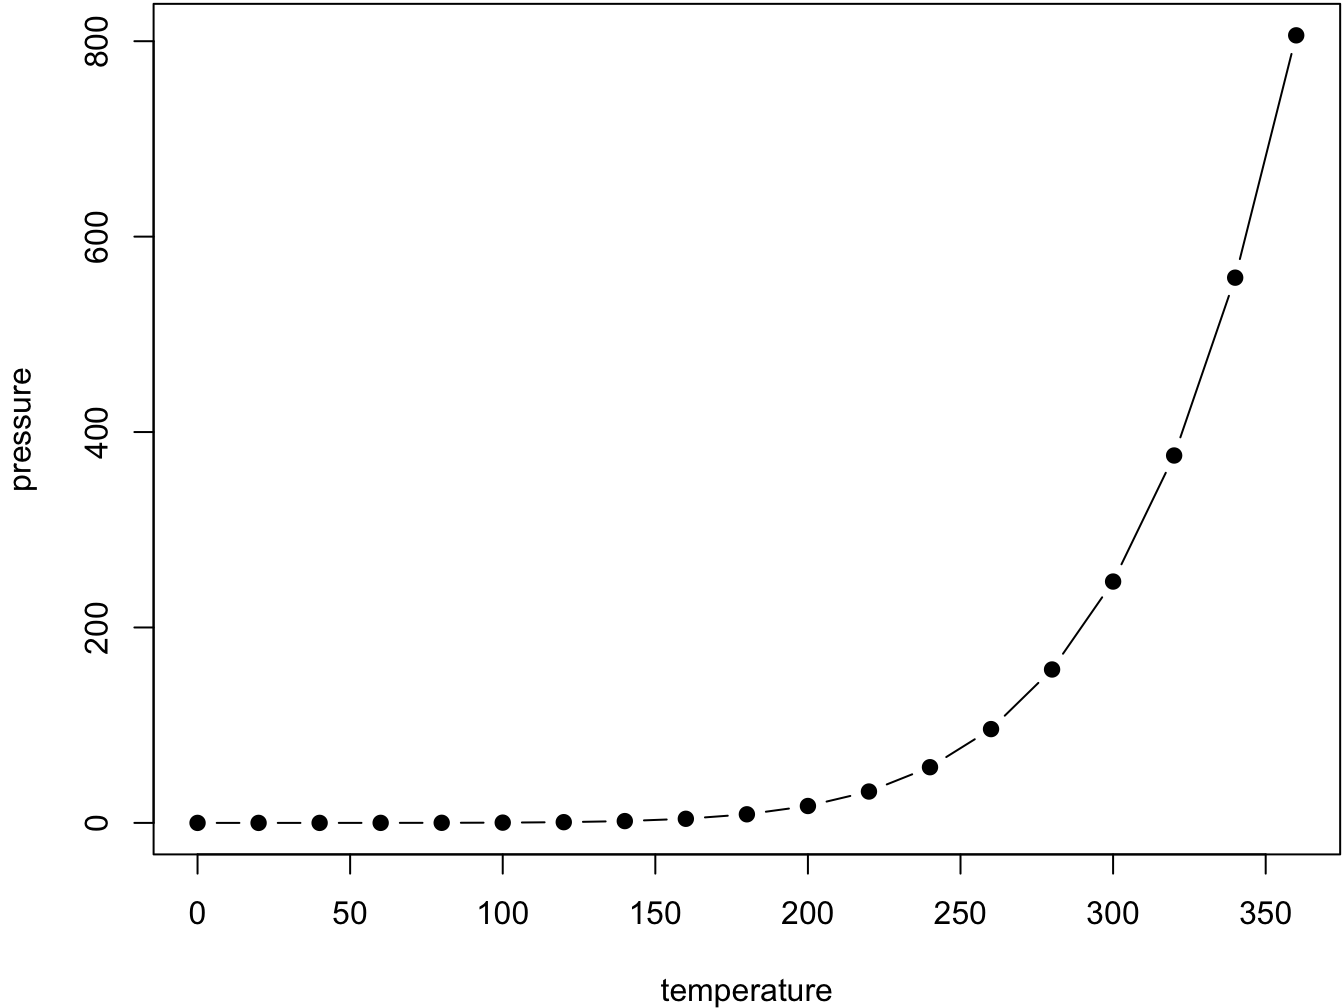
\includegraphics[width=0.8\linewidth]{esds_book_files/figure-latex/nice-fig-1} 

}

\caption{Here is a nice figure!}\label{fig:nice-fig}
\end{figure}

Reference a figure by its code chunk label with the \texttt{fig:} prefix, e.g., see Figure \ref{fig:nice-fig}. Similarly, you can reference tables generated from \texttt{knitr::kable()}, e.g., see Table \ref{tab:nice-tab}.

\begin{Shaded}
\begin{Highlighting}[]
\NormalTok{knitr}\OperatorTok{::}\KeywordTok{kable}\NormalTok{(}
  \KeywordTok{head}\NormalTok{(iris, }\DecValTok{20}\NormalTok{), }\DataTypeTok{caption =} \StringTok{'Here is a nice table!'}\NormalTok{,}
  \DataTypeTok{booktabs =} \OtherTok{TRUE}
\NormalTok{)}
\end{Highlighting}
\end{Shaded}

\begin{table}

\caption{\label{tab:nice-tab}Here is a nice table!}
\centering
\begin{tabular}[t]{rrrrl}
\toprule
Sepal.Length & Sepal.Width & Petal.Length & Petal.Width & Species\\
\midrule
5.1 & 3.5 & 1.4 & 0.2 & setosa\\
4.9 & 3.0 & 1.4 & 0.2 & setosa\\
4.7 & 3.2 & 1.3 & 0.2 & setosa\\
4.6 & 3.1 & 1.5 & 0.2 & setosa\\
5.0 & 3.6 & 1.4 & 0.2 & setosa\\
\addlinespace
5.4 & 3.9 & 1.7 & 0.4 & setosa\\
4.6 & 3.4 & 1.4 & 0.3 & setosa\\
5.0 & 3.4 & 1.5 & 0.2 & setosa\\
4.4 & 2.9 & 1.4 & 0.2 & setosa\\
4.9 & 3.1 & 1.5 & 0.1 & setosa\\
\addlinespace
5.4 & 3.7 & 1.5 & 0.2 & setosa\\
4.8 & 3.4 & 1.6 & 0.2 & setosa\\
4.8 & 3.0 & 1.4 & 0.1 & setosa\\
4.3 & 3.0 & 1.1 & 0.1 & setosa\\
5.8 & 4.0 & 1.2 & 0.2 & setosa\\
\addlinespace
5.7 & 4.4 & 1.5 & 0.4 & setosa\\
5.4 & 3.9 & 1.3 & 0.4 & setosa\\
5.1 & 3.5 & 1.4 & 0.3 & setosa\\
5.7 & 3.8 & 1.7 & 0.3 & setosa\\
5.1 & 3.8 & 1.5 & 0.3 & setosa\\
\bottomrule
\end{tabular}
\end{table}

You can write citations, too. For example, we are using the \textbf{bookdown} package \citep{R-bookdown} in this sample book, which was built on top of R Markdown and \textbf{knitr} \citep{xie2015}.

\hypertarget{data-wrangling}{%
\chapter{Data wrangling}\label{data-wrangling}}

TBC

\hypertarget{data-variety}{%
\chapter{Data variety}\label{data-variety}}

\hypertarget{introduction}{%
\section{Introduction}\label{introduction}}

\hypertarget{overview}{%
\subsection{Overview}\label{overview}}

In this practical we look at data variety in environmental sciences. We start with the data from one eddy covariance measurement site in Switzerland which we had already encountered in Chapter 1, and complement it with a different type of data (remote sensing data). Specifically, we download remote sensing data that measures vegetation greenness data, quantified by the normalised difference vegetation index, NDVI. We are interested in this data for example, because we expect ecosystem photosynthesis (gross primary production), measured at the eddy covariance tower, to covary with NDVI. Such covariation can provide powerful information for modelling. For example, we can train a machine learning model with the observed covariation between measured GPP and NDVI at eddy covariance sites and use that model to scale GPP up in space (NDVI is available for the whole globe, while GPP can only be measured locally.) You will actually be doing this kind of modelling in session 13. For now, we focus on working with the spatial aspects of the data (since remote sensing data is inherently spatial) and introduce you to the toolset to work with spatial, in particular, geo-spatial data.

To get you familiar with spatial data types we will use a variety of data from freely accessible sites. We can investigate abiotic and biotic conditions in these locations. We'll be plotting the Eddy towers you have already encountered in the first two chapters and extracting values for these locations from other data. By doing this we can show that the climate at these sites spans a gradient temperature and landcover. There are also biotic components that could explain variation in productivity among sites, including species composition and functional traits of plants.

\hypertarget{learning-objectives}{%
\subsection{Learning objectives}\label{learning-objectives}}

After this learning unit, you will be able to \ldots{}

\begin{itemize}
\tightlist
\item
  explain the possible sources of data in environmental sciences;
\item
  understand the range of operations applied to data from basic to complex;
\item
  read various types of data in R and apply basic operations;
\item
  understand the structure of spatial data, including rasters and shapefiles;
\item
  apply a range of operations to prepare data for analyses.
\end{itemize}

\hypertarget{key-points-of-the-lecture}{%
\subsection{Key points of the lecture}\label{key-points-of-the-lecture}}

Data operations range in complexity, here they are listed from simplest to extremely complex:

\begin{itemize}
\tightlist
\item
  Statistical operations
\item
  Similarity metrics
\item
  Ordinations
\item
  Clustering
\item
  Classifications
\item
  Regressions
\item
  Neural network deep learning
\end{itemize}

Examples of methods for the computing differences between datasets:

\begin{itemize}
\tightlist
\item
  \emph{Euclidean distance} is used for the simple quantification of variation
\item
  \emph{PCA} is a valuable tool to explore variation and reduce dimension
\item
  \emph{Hamming distance} helps measure the difference between strings
\item
  \emph{Jaccard index} describes the similarity between two or more binary data sets
\end{itemize}

Machine learning is loosely defined as any learning done by a computer. It can be divided into\ldots{}

\begin{itemize}
\tightlist
\item
  \emph{Unsupervised learning}: without explanatory data, which uses clustering to obtain a categorical output
\item
  \emph{Supervised learning}: with explanatory data, which uses either classification also resulting in a categorical output, or regression when a numerical output is required
\end{itemize}

Data errors are divided into errors of accuracy and precision. If data is inaccurate, it strays from the true value. If data is imprecise, individual data points are variable under the same conditions. Systematic errors and inaccurate data is much harder to correct!

Errors can arise throughout the data science workflow.

\begin{itemize}
\tightlist
\item
  \emph{Inherent error} refers to the error present in the source documents and data.
\item
  \emph{Operational error} is created after data collection.
\end{itemize}

Data can be cleaned from errors by looking for:

\begin{itemize}
\tightlist
\item
  Non-uniform data
\item
  Missing data
\item
  Duplicated data
\item
  Outliers
\item
  Measurement errors
\end{itemize}

Quantifying uncertainty is extremely important, as undetectable errors will persist even after data cleaning. Examples of uncertainty quantification include\ldots{}

\begin{itemize}
\tightlist
\item
  Confidence interval (CI)
\item
  Prediction interval
\end{itemize}

Error propagation is used for datasets containing different uncertainties to determine the overall uncertainty.

\hypertarget{tutorial}{%
\section{Tutorial}\label{tutorial}}

\hypertarget{overview-1}{%
\subsection{Overview}\label{overview-1}}

In this practical, you will be downloading and getting to know spatial data. There are three types of spatial data:

\begin{itemize}
\tightlist
\item
  points;
\item
  shapefiles;
\item
  rasters.
\end{itemize}

The first part of this practical is mandatory and will start with a little introduction on downloading remote sensing data for our tower sites and seeing what kinds of information we can gather from this. Then we will get into the nitty-gritty aspects of the afore mentioned spatial data types.

The second part is the bonus part, there we will discuss trait data and the principal component analysis (PCA), which is a method to reduce the dimensions of datasets.

\hypertarget{modis-remote-download}{%
\subsection{MODIS remote download}\label{modis-remote-download}}

We'll be starting off this tutorial with an example on using remote sensing data. We'll focus on a Fluxnet site already familiar to you: CH-Lae. The Lägern site is located on a mountain in the Swiss Plateau NW of Zürich and is surrounded by managed mixed deciduous mountain forests. The forest is highly diverse and dominated by beech. In the following figures, you can get an impression of the tower and its surroundings.

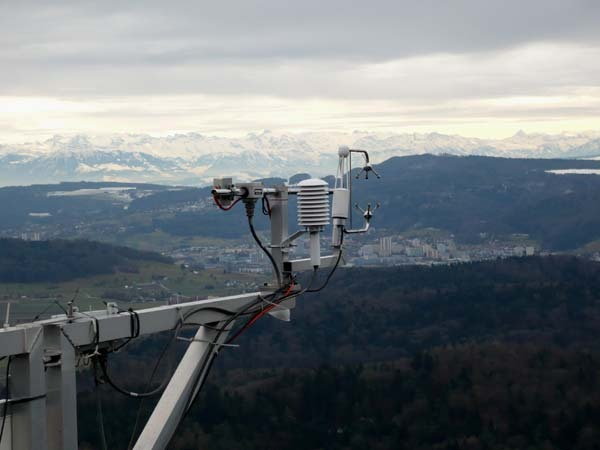
\includegraphics{./figures/site1.jpg}
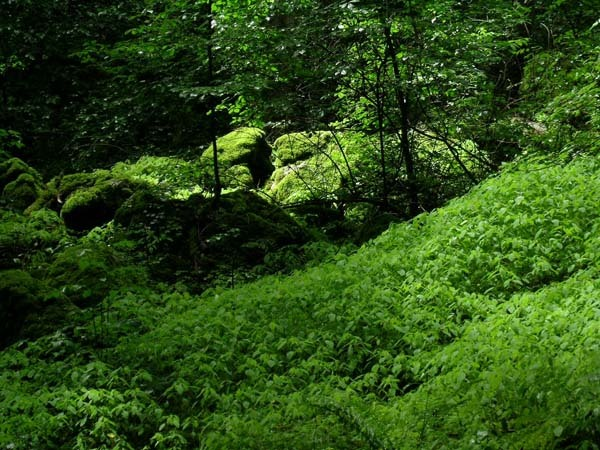
\includegraphics{./figures/site2.jpg}
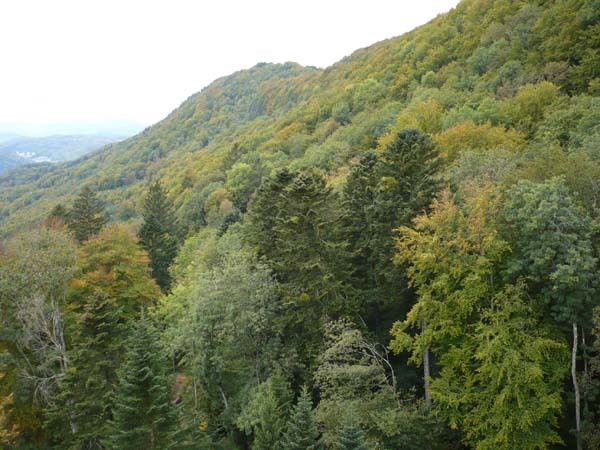
\includegraphics{./figures/site3.jpg}

As always we start by loading \texttt{tidyverse}and our fluxnet site data.

\begin{Shaded}
\begin{Highlighting}[]
\KeywordTok{library}\NormalTok{(tidyverse)}
\NormalTok{df_sites <-}\StringTok{ }\KeywordTok{read_csv}\NormalTok{(}\StringTok{"./data/fluxnet_site_info_reduced.csv"}\NormalTok{)}
\end{Highlighting}
\end{Shaded}

Since for this section we will only be working with the Lägern site we can directly extract its latitude and longitude.

\begin{Shaded}
\begin{Highlighting}[]
\NormalTok{lon_lae <-}\StringTok{ }\NormalTok{df_sites }\OperatorTok\StringTok{ }
\StringTok{  }\KeywordTok{filter}\NormalTok{(site }\OperatorTok{==}\StringTok{ "CH-Lae"}\NormalTok{) }\OperatorTok\StringTok{ }
\StringTok{  }\KeywordTok{pull}\NormalTok{(lon)}

\NormalTok{lat_lae <-}\StringTok{ }\NormalTok{df_sites }\OperatorTok\StringTok{ }
\StringTok{  }\KeywordTok{filter}\NormalTok{(site }\OperatorTok{==}\StringTok{ "CH-Lae"}\NormalTok{) }\OperatorTok\StringTok{ }
\StringTok{  }\KeywordTok{pull}\NormalTok{(lat)}
\end{Highlighting}
\end{Shaded}

In this first analysis, we want to complement temporal data measured by the Fluxnet tower with remote sensing data. \emph{Remote sensing} is the detection or monitoring of physical characteristics of the Earth's surface by measuring reflected and emitted radiation at a distance. Data is collected in the form of images by special cameras typically from aircrafts or satellites. With this method, a huge amount of global data at large spatial scales gets easily accessible and therefore represents a useful method for the monitoring of ecosystems. However, this remotely acquired data requires validation from ground measurements, which can be done for example using the Eddy towers from the previous practicals.

One of these satellite remote sensing instruments is MODIS (Moderate Resolution Imaging Spectroradiometer). Terra MODIS and Aqua MODIS are viewing the entire Earth's surface every 1 to 2 days, acquiring data in 36 spectral bands, or groups of wavelengths.

You used to have to visit an website to be able to download the data file by file, which was a long and tedious process. Luckily, now we have access to tools that make it much more straightforward to download remote sensing data from satellites. It provides Atmosphere, Ocean, Cryosphere and Land data series. The \texttt{MODISTools} package provides a programmatic interface to the \href{https://modis.gsfc.nasa.gov/}{MODIS Land Products Subsets web services} allows for easy downloads of ``MODIS'' time series (of single pixels or small regions of interest) directly to your R workspace or your computer.

\begin{itemize}
\tightlist
\item
  Using the \texttt{mt\_...()} functions of the MODISTools we can check which products are available in MODIS, how the product we are searching for is called, and what temporal and spatial resolutions are available.
\item
  \texttt{t\_products()} lists all available products from MODIS with their temporal and spatial resolution. Products are parent categories of variables measured by the satellites, such as vegetation indices.
\item
  \texttt{mt\_bands()} requires the entry of a product chosen from ``products'' and list the available data variables that are represented by the different actually measured wavelengths.
\item
  Finally, \texttt{mt\_dates()} lists all dates of which data from the chosen product and band are available.
\end{itemize}

We will make use of this by loading NDVI data around our towers directly from MODIS.

\begin{Shaded}
\begin{Highlighting}[]
\KeywordTok{library}\NormalTok{(MODISTools)}
\NormalTok{products <-}\StringTok{ }\KeywordTok{mt_products}\NormalTok{() }\OperatorTok\StringTok{ }\KeywordTok{as_tibble}\NormalTok{()}
\NormalTok{bands <-}\StringTok{ }\KeywordTok{mt_bands}\NormalTok{(}\DataTypeTok{product =} \StringTok{"MOD13Q1"}\NormalTok{) }\OperatorTok\StringTok{ }\KeywordTok{as_tibble}\NormalTok{()}
\NormalTok{dates <-}\StringTok{ }\KeywordTok{mt_dates}\NormalTok{(}\DataTypeTok{product =} \StringTok{"MOD13Q1"}\NormalTok{, }\DataTypeTok{lat =}\NormalTok{ lat_lae, }\DataTypeTok{lon =}\NormalTok{ lon_lae) }\OperatorTok\StringTok{ }\KeywordTok{as_tibble}\NormalTok{()}
\end{Highlighting}
\end{Shaded}

Now, we'll get the NDVI data for 6 years for a square of 2km x 2km around the tower site. We use the function \texttt{mt\_subset()} for this. The parameters of this function download a subset of data within the chosen product (here `MOD13Q1'). We specify the location as latitude and longitude, and the band we chose, which is at 250m spatial resolution and 16-day temporal resolution. The time period can be chosen as a subset of ``dates'' and must be provided in the form of start and end date. We will be looking at the beginning of 2009 to the end of 2014. \texttt{km\_lr} and \texttt{km\_ab} define the kilometers to the left and right of the location and kilometers above and below respectively. Since these values are being rounded to the nearest integer, we chose this minimum of 1, corresponding to 2km2. Sitename is used in writing data to file, internal gives the command whether the data should be returned as an internal structure. The progress setting defines whether the download progress should be shown or not.

\begin{Shaded}
\begin{Highlighting}[]
\NormalTok{df_ndvi <-}\StringTok{ }\KeywordTok{mt_subset}\NormalTok{(}\DataTypeTok{product =} \StringTok{"MOD13Q1"}\NormalTok{,            }\CommentTok{# the chosen product}
                  \DataTypeTok{lat =}\NormalTok{ lat_lae,                     }\CommentTok{# desired lat/lon}
                  \DataTypeTok{lon =}\NormalTok{ lon_lae,}
                  \DataTypeTok{band =} \StringTok{"250m_16_days_NDVI"}\NormalTok{,        }\CommentTok{# chosen band defining spatial and temporal scale}
                  \DataTypeTok{start =} \StringTok{"2009-01-01"}\NormalTok{,              }\CommentTok{# start date: 1st Jan 2009}
                  \DataTypeTok{end =} \StringTok{"2014-12-19"}\NormalTok{,                }\CommentTok{# end date: 19th Dec 2014}
                  \DataTypeTok{km_lr =} \DecValTok{1}\NormalTok{,                         }\CommentTok{# kilometers left & right of the chosen location (lat/lon above)}
                  \DataTypeTok{km_ab =} \DecValTok{1}\NormalTok{,                         }\CommentTok{# kilometers above and below the location}
                  \DataTypeTok{site_name =} \StringTok{"CH-Lae"}\NormalTok{,              }\CommentTok{# the site name we want to give the data}
                  \DataTypeTok{internal =} \OtherTok{TRUE}\NormalTok{,}
                  \DataTypeTok{progress =} \OtherTok{FALSE}
\NormalTok{                  ) }\OperatorTok\StringTok{ }
\StringTok{  }\KeywordTok{as_tibble}\NormalTok{()}
\end{Highlighting}
\end{Shaded}

\begin{Shaded}
\begin{Highlighting}[]
\KeywordTok{head}\NormalTok{(df_ndvi)}
\end{Highlighting}
\end{Shaded}

\begin{verbatim}
## # A tibble: 6 x 21
##   xllcorner yllcorner cellsize nrows ncols band  units scale latitude longitude
##   <chr>     <chr>     <chr>    <int> <int> <chr> <chr> <chr>    <dbl>     <dbl>
## 1 627557.11 5278290.~ 231.656~     9     9 250m~ NDVI~ 0.00~     47.5      8.36
## 2 627557.11 5278290.~ 231.656~     9     9 250m~ NDVI~ 0.00~     47.5      8.36
## 3 627557.11 5278290.~ 231.656~     9     9 250m~ NDVI~ 0.00~     47.5      8.36
## 4 627557.11 5278290.~ 231.656~     9     9 250m~ NDVI~ 0.00~     47.5      8.36
## 5 627557.11 5278290.~ 231.656~     9     9 250m~ NDVI~ 0.00~     47.5      8.36
## 6 627557.11 5278290.~ 231.656~     9     9 250m~ NDVI~ 0.00~     47.5      8.36
## # ... with 11 more variables: site <chr>, product <chr>, start <chr>,
## #   end <chr>, complete <lgl>, modis_date <chr>, calendar_date <chr>,
## #   tile <chr>, proc_date <chr>, pixel <int>, value <int>
\end{verbatim}

This dataframe takes some effort to make sense of. Let's make our lives a little easier and put this data into a useful spatial context. For that it needs to be converted to a raster. This is a key spatial data type and will be described in more detail in the section Raster below.
MODISTools provides a handy integrated function for converting the data to a raster \texttt{mt\_to\_raster()}.

\begin{verbatim}
## Warning in showSRID(uprojargs, format = "PROJ", multiline = "NO", prefer_proj =
## prefer_proj): Discarded ellps unknown in Proj4 definition: +proj=sinu +lon_0=0
## +x_0=0 +y_0=0 +R=6371007.181 +units=m +no_defs +type=crs
\end{verbatim}

\begin{verbatim}
## Warning in showSRID(uprojargs, format = "PROJ", multiline = "NO", prefer_proj =
## prefer_proj): Discarded datum unknown in Proj4 definition
\end{verbatim}

\begin{verbatim}
## Warning in showSRID(SRS_string, format = "PROJ", multiline = "NO", prefer_proj
## = prefer_proj): Discarded ellps unknown in Proj4 definition: +proj=sinu +lon_0=0
## +x_0=0 +y_0=0 +R=6371007.181 +units=m +no_defs +type=crs
\end{verbatim}

\begin{verbatim}
## Warning in showSRID(SRS_string, format = "PROJ", multiline = "NO", prefer_proj =
## prefer_proj): Discarded datum unknown in Proj4 definition
\end{verbatim}

\begin{verbatim}
## Warning in showSRID(uprojargs, format = "PROJ", multiline = "NO", prefer_proj =
## prefer_proj): Discarded ellps unknown in Proj4 definition: +proj=sinu +lon_0=0
## +x_0=0 +y_0=0 +R=6371007.181 +units=m +no_defs +type=crs
\end{verbatim}

\begin{verbatim}
## Warning in showSRID(uprojargs, format = "PROJ", multiline = "NO", prefer_proj =
## prefer_proj): Discarded datum unknown in Proj4 definition
\end{verbatim}

By plotting the data we can verify that we loaded a square of NDVI data around our tower for every 16-day time step.
We plot four images in the winter season.

\begin{Shaded}
\begin{Highlighting}[]
\KeywordTok{plot}\NormalTok{(raster_ndvi[[}\DecValTok{1}\OperatorTok{:}\DecValTok{4}\NormalTok{]], }\DataTypeTok{zlim=}\KeywordTok{c}\NormalTok{(}\OperatorTok{-}\FloatTok{0.1}\NormalTok{, }\FloatTok{0.95}\NormalTok{))}
\end{Highlighting}
\end{Shaded}

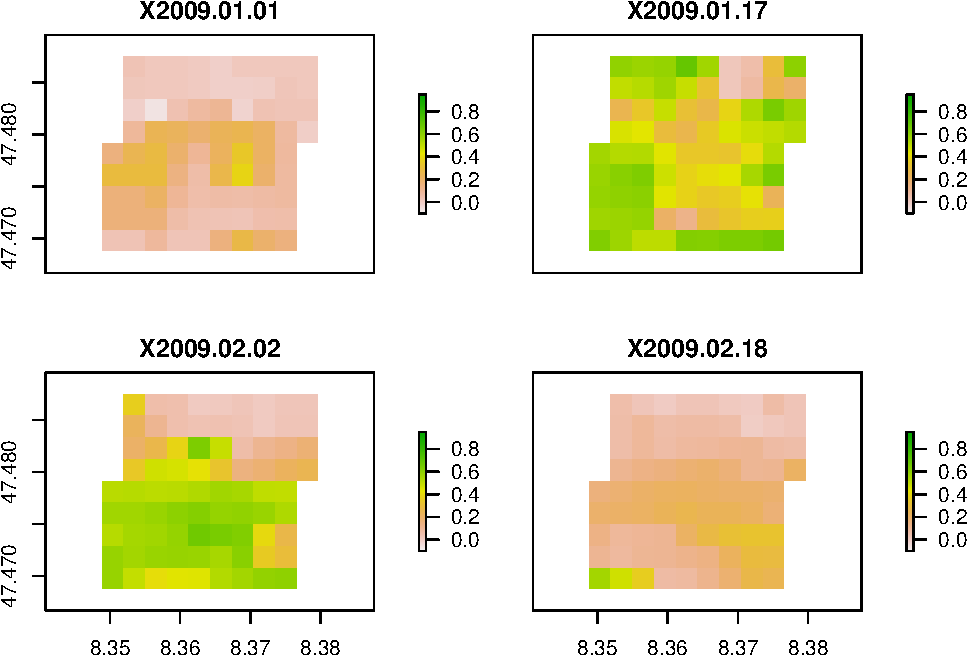
\includegraphics{esds_book_files/figure-latex/unnamed-chunk-10-1.pdf}

Just out of interest let's calculate the minimum and maximum of these plots.

\begin{Shaded}
\begin{Highlighting}[]
\NormalTok{min_winter <-}\StringTok{ }\KeywordTok{min}\NormalTok{(}\KeywordTok{minValue}\NormalTok{(raster_ndvi[[}\DecValTok{1}\OperatorTok{:}\DecValTok{4}\NormalTok{]]))}
\NormalTok{max_winter <-}\StringTok{ }\KeywordTok{max}\NormalTok{(}\KeywordTok{maxValue}\NormalTok{(raster_ndvi[[}\DecValTok{1}\OperatorTok{:}\DecValTok{4}\NormalTok{]]))}
\KeywordTok{paste0}\NormalTok{(}\StringTok{"Minimum Winter:"}\NormalTok{, }\DataTypeTok{sep=}\StringTok{" "}\NormalTok{, min_winter)}
\end{Highlighting}
\end{Shaded}

\begin{verbatim}
## [1] "Minimum Winter: -0.0679177447153291"
\end{verbatim}

\begin{Shaded}
\begin{Highlighting}[]
\KeywordTok{paste0}\NormalTok{(}\StringTok{"Maximum Winter:"}\NormalTok{, }\DataTypeTok{sep=}\StringTok{" "}\NormalTok{, max_winter)}
\end{Highlighting}
\end{Shaded}

\begin{verbatim}
## [1] "Maximum Winter: 0.683717115657303"
\end{verbatim}

We do the same for the summer season.

\begin{Shaded}
\begin{Highlighting}[]
\KeywordTok{plot}\NormalTok{(raster_ndvi[[}\DecValTok{13}\OperatorTok{:}\DecValTok{16}\NormalTok{]], }\DataTypeTok{zlim=}\KeywordTok{c}\NormalTok{(}\OperatorTok{-}\FloatTok{0.1}\NormalTok{, }\FloatTok{0.95}\NormalTok{))}
\end{Highlighting}
\end{Shaded}

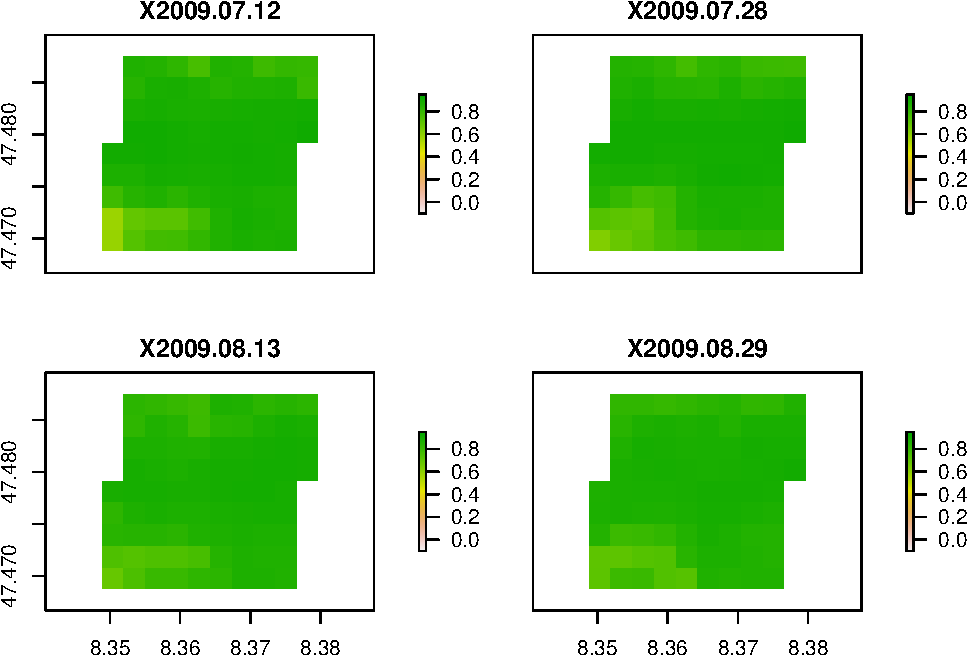
\includegraphics{esds_book_files/figure-latex/unnamed-chunk-12-1.pdf}

We compute minimum and maximum.

\begin{Shaded}
\begin{Highlighting}[]
\NormalTok{min_summer <-}\StringTok{ }\KeywordTok{min}\NormalTok{(}\KeywordTok{minValue}\NormalTok{(raster_ndvi[[}\DecValTok{13}\OperatorTok{:}\DecValTok{16}\NormalTok{]]))}
\NormalTok{max_summer <-}\StringTok{ }\KeywordTok{max}\NormalTok{(}\KeywordTok{maxValue}\NormalTok{(raster_ndvi[[}\DecValTok{13}\OperatorTok{:}\DecValTok{16}\NormalTok{]]))}
\KeywordTok{paste0}\NormalTok{(}\StringTok{"Minimum Summer:"}\NormalTok{, }\DataTypeTok{sep=}\StringTok{" "}\NormalTok{, min_summer)}
\end{Highlighting}
\end{Shaded}

\begin{verbatim}
## [1] "Minimum Summer: 0.569610980491112"
\end{verbatim}

\begin{Shaded}
\begin{Highlighting}[]
\KeywordTok{paste0}\NormalTok{(}\StringTok{"Maximum Summer:"}\NormalTok{, }\DataTypeTok{sep=}\StringTok{" "}\NormalTok{, max_summer)}
\end{Highlighting}
\end{Shaded}

\begin{verbatim}
## [1] "Maximum Summer: 0.903467898529256"
\end{verbatim}

From the two plots, we can clearly distinguish summer and winter time steps due to the differences in NDVI. Summer NDVI is much higher since our tower site is located in the Northern hemisphere where leaves get lost during winter for many vegetation types. Heterogeneity in winter is higher which might be due to conifers that don't lose their leaves.

However, we are also interested in the mean across all (spatial) pixels for each date. To clarify this means we collapse the pixel dimension into a single mean value for each date. This is can done using \texttt{group\_by()} in combination with \texttt{summarise()}, which were explained in chapter 2.

\begin{Shaded}
\begin{Highlighting}[]
\KeywordTok{library}\NormalTok{(lubridate) }\CommentTok{# lubridate is loaded to work with dates}

\CommentTok{## first determine the scaling factor that is to be applied to the NDVI values. This has practical reasons: reduces disk space}
\NormalTok{scale_factor <-}\StringTok{ }\NormalTok{bands }\OperatorTok\StringTok{ }
\StringTok{  }\KeywordTok{filter}\NormalTok{(band }\OperatorTok{==}\StringTok{ "250m_16_days_NDVI"}\NormalTok{) }\OperatorTok\StringTok{ }
\StringTok{  }\KeywordTok{pull}\NormalTok{(scale_factor) }\OperatorTok\StringTok{ }
\StringTok{  }\KeywordTok{as.numeric}\NormalTok{()}
  
\NormalTok{df_ndvi_spatialmean <-}\StringTok{ }\NormalTok{df_ndvi }\OperatorTok\StringTok{ }
\StringTok{  }\KeywordTok{mutate}\NormalTok{(}\DataTypeTok{calendar_date =} \KeywordTok{ymd}\NormalTok{(calendar_date)) }\OperatorTok\StringTok{  }\CommentTok{# make the dates into comprehensible values not X.yyyy.mm.dd}
\StringTok{  }\KeywordTok{group_by}\NormalTok{(calendar_date) }\OperatorTok\StringTok{                     }\CommentTok{# group the data by day }
\StringTok{  }\KeywordTok{summarise}\NormalTok{(}\DataTypeTok{mean =} \KeywordTok{mean}\NormalTok{(value), }\DataTypeTok{min =} \KeywordTok{min}\NormalTok{(value), }\DataTypeTok{max =} \KeywordTok{max}\NormalTok{(value)) }\OperatorTok\StringTok{   }\CommentTok{# calculate mean, min and max across pixels}
\StringTok{  }\KeywordTok{mutate}\NormalTok{(}\DataTypeTok{mean =}\NormalTok{ mean }\OperatorTok{*}\StringTok{ }\NormalTok{scale_factor, }\DataTypeTok{min =}\NormalTok{ min }\OperatorTok{*}\StringTok{ }\NormalTok{scale_factor, }\DataTypeTok{max =}\NormalTok{ max }\OperatorTok{*}\StringTok{ }\NormalTok{scale_factor)  }\CommentTok{# apply scale_factor (see )}
\end{Highlighting}
\end{Shaded}

We can now plot our NDVI time series across our years (2009 to 2014) using the means we calculated above.

\begin{Shaded}
\begin{Highlighting}[]
\NormalTok{df_ndvi_spatialmean }\OperatorTok\StringTok{ }
\StringTok{  }\KeywordTok{ggplot}\NormalTok{(}\KeywordTok{aes}\NormalTok{(}\DataTypeTok{x =}\NormalTok{ calendar_date)) }\OperatorTok{+}
\StringTok{  }\KeywordTok{geom_ribbon}\NormalTok{(}\KeywordTok{aes}\NormalTok{(}\DataTypeTok{ymin =}\NormalTok{ min, }\DataTypeTok{ymax =}\NormalTok{ max), }\DataTypeTok{fill =} \StringTok{"grey70"}\NormalTok{) }\OperatorTok{+}
\StringTok{  }\KeywordTok{geom_line}\NormalTok{(}\KeywordTok{aes}\NormalTok{(}\DataTypeTok{y =}\NormalTok{ mean))}
\end{Highlighting}
\end{Shaded}

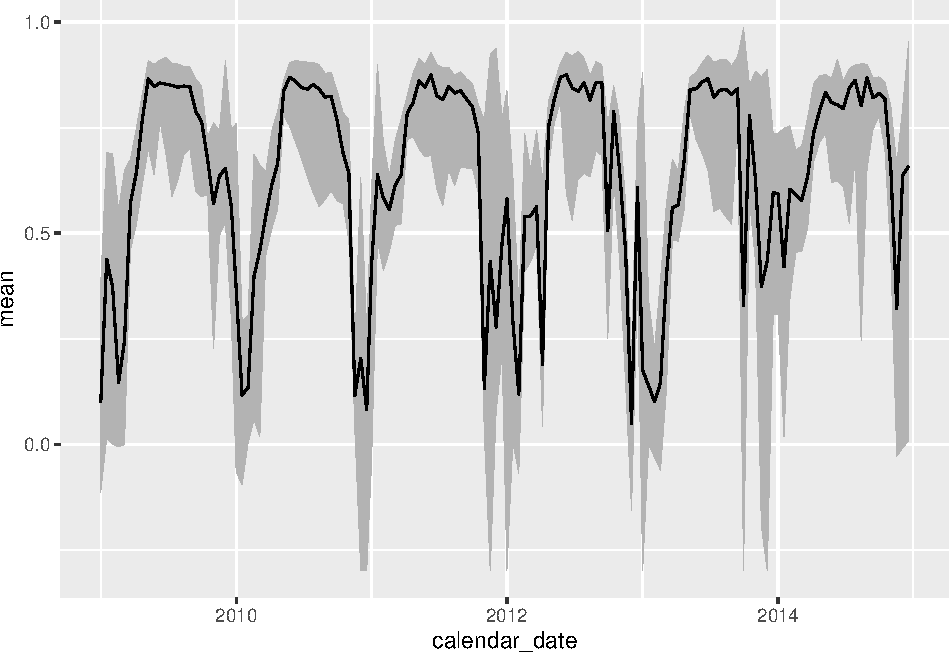
\includegraphics{esds_book_files/figure-latex/unnamed-chunk-15-1.pdf}

After having aggregated the data to the mean NDVI across all 81 pixels for each date, we have reduced the dimensions of the data frame to only one (time). It now has a structure that can easily be combined with the time series data from the eddy covariance tower (each site is a point in space).

\begin{Shaded}
\begin{Highlighting}[]
\CommentTok{# this can now be combined to the data frame with flux data that also has dates along rows}
\NormalTok{ddf_ch_lae <-}\StringTok{ }\KeywordTok{read_csv}\NormalTok{(}\StringTok{"./data/ddf_ch_lae.csv"}\NormalTok{)}
\end{Highlighting}
\end{Shaded}

\begin{Shaded}
\begin{Highlighting}[]
\CommentTok{# now we can combine the two data frames along dates. }
\NormalTok{ddf_ch_lae_ndvi <-}\StringTok{ }\NormalTok{ddf_ch_lae }\OperatorTok
\StringTok{  }\NormalTok{dplyr}\OperatorTok{::}\KeywordTok{rename}\NormalTok{(}\DataTypeTok{date =}\NormalTok{ TIMESTAMP) }\OperatorTok\StringTok{ }
\StringTok{  }\NormalTok{dplyr}\OperatorTok{::}\KeywordTok{mutate}\NormalTok{(}\DataTypeTok{year =} \KeywordTok{year}\NormalTok{(date)) }\OperatorTok\StringTok{ }
\StringTok{  }\NormalTok{dplyr}\OperatorTok{::}\KeywordTok{filter}\NormalTok{(year }\OperatorTok\StringTok{ }\DecValTok{2009}\OperatorTok{:}\DecValTok{2014}\NormalTok{) }\OperatorTok\StringTok{  }\CommentTok{# NDVI data was downloaded only for these years}
\StringTok{  }\KeywordTok{left_join}\NormalTok{(df_ndvi_spatialmean }\OperatorTok\StringTok{ }\KeywordTok{rename}\NormalTok{(}\DataTypeTok{date =}\NormalTok{ calendar_date), }\DataTypeTok{by =} \StringTok{"date"}\NormalTok{) }\OperatorTok\StringTok{ }
\StringTok{  }\NormalTok{dplyr}\OperatorTok{::}\KeywordTok{select}\NormalTok{(}\OperatorTok{-}\NormalTok{year)}
\end{Highlighting}
\end{Shaded}

NDVI data is provided every 16 days. In order to predict values at other time steps, we can fit a cubic smoothing spline to our daily values. (Cubic smoothing splines embody a curve fitting technique that blends the ideas of cubic splines and curvature minimization to create an effective data modeling tool for noisy data. Traditional interpolating cubic splines represent the tabulated data as a piece-wise continuous curve which passes through each value in the data table. The curve spanning each data interval is represented by a cubic polynomial, with the requirement that the endpoints of adjacent cubic polynomials match in location and in their first and second derivatives).

\begin{Shaded}
\begin{Highlighting}[]
\NormalTok{ddf_ch_lae_ndvi <-}\StringTok{ }\NormalTok{ddf_ch_lae_ndvi }\OperatorTok\StringTok{ }
\StringTok{  }\KeywordTok{mutate}\NormalTok{(}\DataTypeTok{date_dec =} \KeywordTok{decimal_date}\NormalTok{(date))}

\NormalTok{df_nona <-}\StringTok{ }\NormalTok{ddf_ch_lae_ndvi }\OperatorTok\StringTok{ }
\StringTok{  }\KeywordTok{drop_na}\NormalTok{()}

\NormalTok{out_spline <-}\StringTok{ }\KeywordTok{smooth.spline}\NormalTok{( df_nona}\OperatorTok{$}\NormalTok{date_dec, df_nona}\OperatorTok{$}\NormalTok{mean, }\DataTypeTok{spar=}\FloatTok{0.1}\NormalTok{ )}
\NormalTok{vals_spline <-}\StringTok{ }\KeywordTok{predict}\NormalTok{( out_spline, ddf_ch_lae_ndvi}\OperatorTok{$}\NormalTok{date_dec )}\OperatorTok{$}\NormalTok{y}

\NormalTok{ddf_ch_lae_ndvi <-}\StringTok{ }\NormalTok{ddf_ch_lae_ndvi }\OperatorTok\StringTok{ }
\StringTok{  }\KeywordTok{mutate}\NormalTok{(}\DataTypeTok{ndvi_splined =}\NormalTok{ vals_spline)}
\end{Highlighting}
\end{Shaded}

Let's take a look\ldots{}

\begin{Shaded}
\begin{Highlighting}[]
\NormalTok{ddf_ch_lae_ndvi }\OperatorTok\StringTok{ }
\StringTok{  }\KeywordTok{ggplot}\NormalTok{() }\OperatorTok{+}
\StringTok{  }\KeywordTok{geom_point}\NormalTok{(}\KeywordTok{aes}\NormalTok{(}\DataTypeTok{x =}\NormalTok{ date, }\DataTypeTok{y =}\NormalTok{ mean)) }\OperatorTok{+}
\StringTok{  }\KeywordTok{geom_line}\NormalTok{(}\KeywordTok{aes}\NormalTok{(}\DataTypeTok{x =}\NormalTok{ date, }\DataTypeTok{y =}\NormalTok{ ndvi_splined), }\DataTypeTok{color =} \StringTok{"red"}\NormalTok{)}
\end{Highlighting}
\end{Shaded}

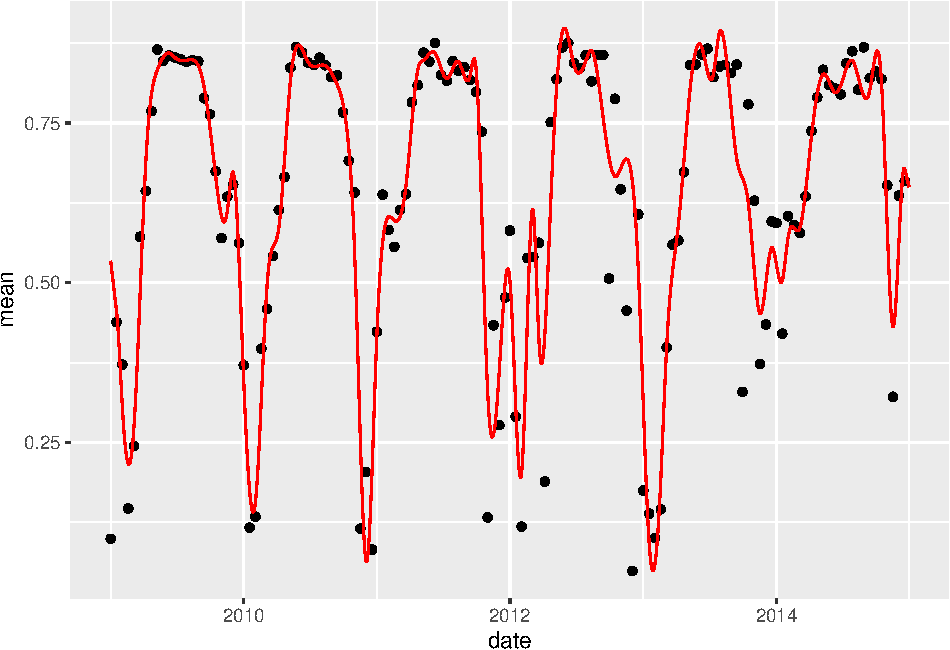
\includegraphics{esds_book_files/figure-latex/unnamed-chunk-19-1.pdf}

To see how well this data correlates with measurements from the fluxnet tower, we look at the relationship of GPP vs.~NDVI*PPFD.

\begin{Shaded}
\begin{Highlighting}[]
\NormalTok{ddf_ch_lae_ndvi <-}\StringTok{ }\NormalTok{ddf_ch_lae_ndvi }\OperatorTok\StringTok{ }
\StringTok{  }\KeywordTok{mutate}\NormalTok{(}\DataTypeTok{ppfd_abs =}\NormalTok{ ndvi_splined }\OperatorTok{*}\StringTok{ }\NormalTok{PPFD_IN)}
\end{Highlighting}
\end{Shaded}

Does NDVI affect the relationship between GPP and PPFD?

\begin{Shaded}
\begin{Highlighting}[]
\NormalTok{linmod1 <-}\StringTok{ }\KeywordTok{lm}\NormalTok{(GPP_NT_VUT_REF }\OperatorTok{~}\StringTok{ }\NormalTok{PPFD_IN, }\DataTypeTok{data =}\NormalTok{ ddf_ch_lae_ndvi)}
\KeywordTok{summary}\NormalTok{(linmod1)}
\end{Highlighting}
\end{Shaded}

\begin{verbatim}
## 
## Call:
## lm(formula = GPP_NT_VUT_REF ~ PPFD_IN, data = ddf_ch_lae_ndvi)
## 
## Residuals:
##      Min       1Q   Median       3Q      Max 
## -10.3749  -2.0413  -0.0137   1.9913  14.8576 
## 
## Coefficients:
##              Estimate Std. Error t value Pr(>|t|)    
## (Intercept) 0.9348433  0.1097112   8.521   <2e-16 ***
## PPFD_IN     0.0148270  0.0003038  48.797   <2e-16 ***
## ---
## Signif. codes:  0 '***' 0.001 '**' 0.01 '*' 0.05 '.' 0.1 ' ' 1
## 
## Residual standard error: 3.06 on 2173 degrees of freedom
##   (16 observations deleted due to missingness)
## Multiple R-squared:  0.5229, Adjusted R-squared:  0.5226 
## F-statistic:  2381 on 1 and 2173 DF,  p-value: < 2.2e-16
\end{verbatim}

\begin{Shaded}
\begin{Highlighting}[]
\NormalTok{linmod2 <-}\StringTok{ }\KeywordTok{lm}\NormalTok{(GPP_NT_VUT_REF }\OperatorTok{~}\StringTok{ }\NormalTok{ppfd_abs, }\DataTypeTok{data =}\NormalTok{ ddf_ch_lae_ndvi)}
\KeywordTok{summary}\NormalTok{(linmod2)}
\end{Highlighting}
\end{Shaded}

\begin{verbatim}
## 
## Call:
## lm(formula = GPP_NT_VUT_REF ~ ppfd_abs, data = ddf_ch_lae_ndvi)
## 
## Residuals:
##     Min      1Q  Median      3Q     Max 
## -8.9202 -1.8307 -0.0829  1.7236 14.4273 
## 
## Coefficients:
##              Estimate Std. Error t value Pr(>|t|)    
## (Intercept) 1.3395678  0.0903180   14.83   <2e-16 ***
## ppfd_abs    0.0180868  0.0003148   57.45   <2e-16 ***
## ---
## Signif. codes:  0 '***' 0.001 '**' 0.01 '*' 0.05 '.' 0.1 ' ' 1
## 
## Residual standard error: 2.792 on 2173 degrees of freedom
##   (16 observations deleted due to missingness)
## Multiple R-squared:  0.603,  Adjusted R-squared:  0.6028 
## F-statistic:  3301 on 1 and 2173 DF,  p-value: < 2.2e-16
\end{verbatim}

Indeed, R2 increased from 0.5229 to 0.603 when including considering NDVI * PPFD, instead of just PPFD. In other words, it also matters whether leaves are actually out and green for modelling the relationship between GPP and PPFD. NDVI * PPFD approximates the amount of \emph{absorbed} incoming light (not just the incoming light) and is therefore closer to being a physiologically relevant quantity.

\hypertarget{points-on-the-globe}{%
\subsection{Points on the globe}\label{points-on-the-globe}}

Documenting the coordinates of data as it is collected allows us to assign a precise location to that data, which can be important in further analysis when, for example, comparing location. As you all undoubtedly know coordinates come with a latitude (defining the position N or S of the equator) and longitude (defining the position E or W of the meridian). With the coordinates we can already plot our data points, remembering that the latitude is equivalent to the y-axis and longitude to the x-axis.

In this section, we look at the position of the Fluxnet sites. The Fluxnet network measures land-atmosphere exchanges of greenhouse gases and energy for sites across the globe using the eddy covariance technique. High-frequency measurements of vertical wind velocity and a scalar mixing ratio (CO2, H2O, temperature, etc.) provides estimates of the net exchange of the scalar. Eddy covariance is currently the standard method to measure fluxes of trace gases between ecosystems and the atmosphere (sources:
\url{https://fluxnet.org/about/}, \url{https://www.nature.com/articles/s41597-020-0534-3.pdf}).

Right at the beginning of this tutorial we loaded the dataset containing information on sites in Europe. We treat site locations as a geographical position. So we will extract the name, longitude and latitude of our sites.

\begin{Shaded}
\begin{Highlighting}[]
\KeywordTok{head}\NormalTok{(df_sites)}
\end{Highlighting}
\end{Shaded}

\begin{verbatim}
## # A tibble: 6 x 3
##   site     lon   lat
##   <chr>  <dbl> <dbl>
## 1 BE-Bra  4.52  51.3
## 2 BE-Lon  4.75  50.6
## 3 BE-Vie  6.00  50.3
## 4 CH-Cha  8.41  47.2
## 5 CH-Fru  8.54  47.1
## 6 CH-Lae  8.36  47.5
\end{verbatim}

Our dataset \emph{`df\_sites'} contains two sites in Greenland and Siberia. We'll focus on a smaller spatial domain, restricted to ``mainland'' Europe, therefore, we exclude sites RU-Cok and DK-ZaH.

\begin{Shaded}
\begin{Highlighting}[]
\NormalTok{df_sites <-}\StringTok{ }\NormalTok{df_sites }\OperatorTok\StringTok{ }
\StringTok{  }\KeywordTok{filter}\NormalTok{(}\OperatorTok{!}\NormalTok{(site }\OperatorTok\StringTok{ }\KeywordTok{c}\NormalTok{(}\StringTok{"RU-Cok"}\NormalTok{, }\StringTok{"DK-ZaH"}\NormalTok{)))}
\end{Highlighting}
\end{Shaded}

Already now we can plot our data points without any further adjustments.

\begin{Shaded}
\begin{Highlighting}[]
\KeywordTok{ggplot}\NormalTok{() }\OperatorTok{+}
\StringTok{  }\KeywordTok{geom_point}\NormalTok{(}\DataTypeTok{data =}\NormalTok{ df_sites, }\KeywordTok{aes}\NormalTok{(}\DataTypeTok{x =}\NormalTok{ lon, }\DataTypeTok{y =}\NormalTok{ lat), }\DataTypeTok{color =} \StringTok{"red"}\NormalTok{) }\OperatorTok{+}
\StringTok{  }\KeywordTok{labs}\NormalTok{(}\DataTypeTok{title =} \StringTok{"Selected FLUXNET sites"}\NormalTok{, }\DataTypeTok{x =} \StringTok{"Longitude"}\NormalTok{, }\DataTypeTok{y =} \StringTok{"Latitude"}\NormalTok{)}\OperatorTok{+}
\StringTok{  }\KeywordTok{theme_bw}\NormalTok{()}
\end{Highlighting}
\end{Shaded}

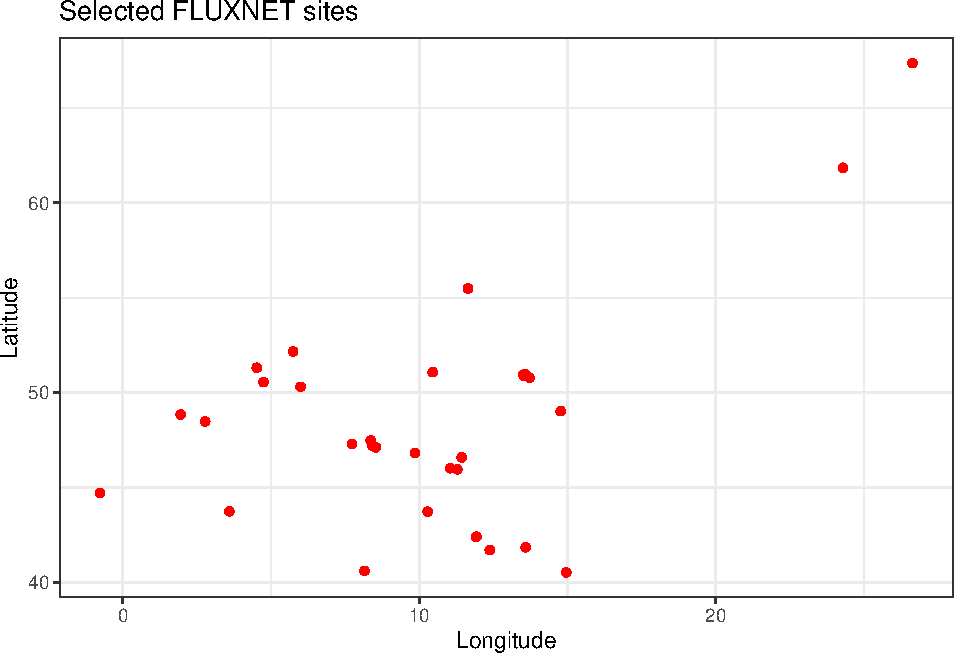
\includegraphics{esds_book_files/figure-latex/unnamed-chunk-25-1.pdf}

We can make an educated guess where the points are but this plot doesn't tell us much by itself without a map as a reference.

So to visualize the location of our points we plot them on a map. We use the package \texttt{SpData} to get the world map and crop it to Europe.

\begin{Shaded}
\begin{Highlighting}[]
\KeywordTok{library}\NormalTok{(sf)}
\KeywordTok{library}\NormalTok{(spData)}
\end{Highlighting}
\end{Shaded}

\begin{verbatim}
## To access larger datasets in this package, install the spDataLarge
## package with: `install.packages('spDataLarge',
## repos='https://nowosad.github.io/drat/', type='source')`
\end{verbatim}

\begin{Shaded}
\begin{Highlighting}[]
\KeywordTok{ggplot}\NormalTok{() }\OperatorTok{+}
\StringTok{  }\KeywordTok{geom_sf}\NormalTok{(}\DataTypeTok{data =}\NormalTok{ world) }\OperatorTok{+}
\StringTok{  }\KeywordTok{geom_point}\NormalTok{(}\DataTypeTok{data =}\NormalTok{ df_sites, }\KeywordTok{aes}\NormalTok{(}\DataTypeTok{x =}\NormalTok{ lon, }\DataTypeTok{y =}\NormalTok{ lat), }\DataTypeTok{color =} \StringTok{"red"}\NormalTok{) }\OperatorTok{+}
\StringTok{  }\KeywordTok{labs}\NormalTok{(}\DataTypeTok{x =} \StringTok{"Longitude"}\NormalTok{, }\DataTypeTok{y =} \StringTok{"Latitude"}\NormalTok{) }\OperatorTok{+}
\StringTok{  }\KeywordTok{coord_sf}\NormalTok{(}\DataTypeTok{xlim =} \KeywordTok{c}\NormalTok{(}\OperatorTok{-}\DecValTok{30}\NormalTok{,}\DecValTok{40}\NormalTok{), }\DataTypeTok{ylim =} \KeywordTok{c}\NormalTok{(}\DecValTok{35}\NormalTok{,}\DecValTok{80}\NormalTok{), }\DataTypeTok{expand =} \OtherTok{FALSE}\NormalTok{) }\OperatorTok{+}
\StringTok{  }\KeywordTok{theme_bw}\NormalTok{()}
\end{Highlighting}
\end{Shaded}

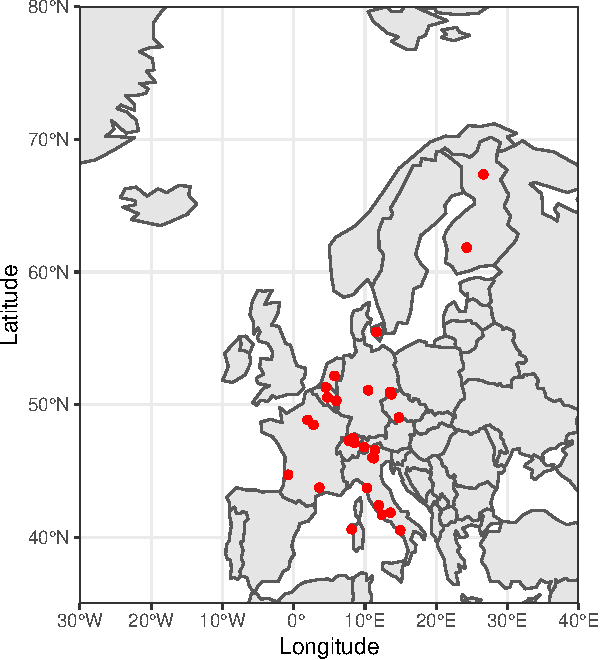
\includegraphics{esds_book_files/figure-latex/unnamed-chunk-26-1.pdf}

\begin{Shaded}
\begin{Highlighting}[]
  \CommentTok{# coord_sf(crs = "+proj=robin")}
\end{Highlighting}
\end{Shaded}

Of course, we can carry on using the data points as they are (for plotting or analysis) but for more detailed spatial analysis we will turn them into \emph{SpatialPoints}.

\emph{SpatialPoints} consist of a matrix with \emph{n} rows and 2 columns, one for each coordinate (latitude \& longitude). \emph{n} is the number of points in the data. These points also have a so-called \emph{`projection string'} or \emph{`crs'} indicating the coordinate reference system in which coordinates of points are expressed.
There are different ways (formulas) to project the earth (an ellipsoid) onto a 2-dimensional map. You can only perform calculations, if the same method (projection, coordinate reference system (crs)) is used. Having points in different coordinate reference systems can cause data to look very skewed. It's good to know which coordinate reference system your data is in, the most commonly used one is \textbf{WGS84 (EPSG: 4326)}. There are some useful resources to convert help you find the correct \href{https://spatialreference.org/ref/epsg/4326/}{spatial reference}.

To transform points into \emph{SpatialPoints} we use the function \texttt{SpatialPoints} in the r package \texttt{sp}.

\begin{Shaded}
\begin{Highlighting}[]
\KeywordTok{library}\NormalTok{(sp)}
\NormalTok{sp_sites <-}\StringTok{ }\KeywordTok{SpatialPoints}\NormalTok{(dplyr}\OperatorTok{::}\KeywordTok{select}\NormalTok{(df_sites, }\OperatorTok{-}\NormalTok{site)) }\CommentTok{# remove character column}
\end{Highlighting}
\end{Shaded}

Below you can see how with the R-base call \texttt{plot()} you can plot the \emph{SpatialPoints} directly. But we'll have to also provide a map to plot them onto. The loaded shapefile of europe will also be used in the next part called Shapefiles.

\begin{Shaded}
\begin{Highlighting}[]
\KeywordTok{library}\NormalTok{(rgdal)}
\NormalTok{europe_shape <-}\StringTok{ }\KeywordTok{readOGR}\NormalTok{(}\DataTypeTok{dsn=}\StringTok{"./data/shapefiles"}\NormalTok{, }\DataTypeTok{layer=}\StringTok{"europe_map"}\NormalTok{)}
\end{Highlighting}
\end{Shaded}

\begin{verbatim}
## OGR data source with driver: ESRI Shapefile 
## Source: "/Users/pascalschneider/Polybox/Shared/Data Science Lecture Planning - shared folder/4 Datasets/shapefiles", layer: "europe_map"
## with 53 features
## It has 94 fields
\end{verbatim}

\begin{Shaded}
\begin{Highlighting}[]
\KeywordTok{plot}\NormalTok{(europe_shape, }\DataTypeTok{col=}\StringTok{"grey"}\NormalTok{)}
\KeywordTok{plot}\NormalTok{(sp_sites, }\DataTypeTok{col =} \StringTok{"red"}\NormalTok{, }\DataTypeTok{add =} \OtherTok{TRUE}\NormalTok{, }\DataTypeTok{pch =} \DecValTok{16}\NormalTok{)}
\end{Highlighting}
\end{Shaded}

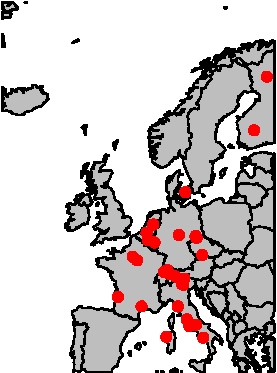
\includegraphics{esds_book_files/figure-latex/unnamed-chunk-28-1.pdf}

\hypertarget{shapefiles}{%
\subsection{Shapefiles}\label{shapefiles}}

Above we looked at points on the globe and transformed our data to \emph{SpatialPoints}. This was already the first example of what forms a shapefile can come in. Shapefiles basically store geographic information, meaning location and any additional information, in shape objects. Shape objects in R are defined by \emph{SpatialPoints}, \emph{SpatialLines}, and \emph{SpatialPolygons} classes of the \texttt{sp} package. The corresponding \emph{SpatialPointsDataFrame}, \emph{SpatialLinesDataFrame}, and \emph{SpatialPolygonsDataFrame} classes allow storing shape objects together with a dataframe. The number of rows in the dataframe corresponds to the number of points (number of rows in coordinate matrix), lines (size of the list of Lines), or polygons (size of the list of Polygons). This allows us to associate a vector of variables (a row of the dataframe) to each shape object.
In the next step, we load a shapefile containing the countries of the world provided by \href{www.naturalearthdata.com}{Natural Earth}, as a reference with which we can contextualize our spatial data. Since we only are looking at towers in Europe, we have cropped the raster to Europe for you.

\begin{Shaded}
\begin{Highlighting}[]
\KeywordTok{library}\NormalTok{(rgdal)}
\NormalTok{europe_shape <-}\StringTok{ }\KeywordTok{readOGR}\NormalTok{(}\DataTypeTok{dsn=}\StringTok{"./data/shapefiles"}\NormalTok{, }\DataTypeTok{layer=}\StringTok{"europe_map"}\NormalTok{)}
\end{Highlighting}
\end{Shaded}

\begin{verbatim}
## OGR data source with driver: ESRI Shapefile 
## Source: "/Users/pascalschneider/Polybox/Shared/Data Science Lecture Planning - shared folder/4 Datasets/shapefiles", layer: "europe_map"
## with 53 features
## It has 94 fields
\end{verbatim}

Let's see what class \emph{europe\_shape} is:

\begin{Shaded}
\begin{Highlighting}[]
\KeywordTok{class}\NormalTok{(europe_shape)}
\end{Highlighting}
\end{Shaded}

\begin{verbatim}
## [1] "SpatialPolygonsDataFrame"
## attr(,"package")
## [1] "sp"
\end{verbatim}

Above we mentioned that \emph{SpatialPolygonsDataFrame} contains both a list of \emph{SpatialPolygons} and a dataframe with information on each polygon. Here's how you can access the information in the dataframe. We'll just display the header for now.

\begin{Shaded}
\begin{Highlighting}[]
\KeywordTok{head}\NormalTok{(europe_shape}\OperatorTok{@}\NormalTok{data)}
\end{Highlighting}
\end{Shaded}

\begin{verbatim}
##        featurecla scalerank LABELRANK     SOVEREIGNT SOV_A3 ADM0_DIF LEVEL
## 0 Admin-0 country         6         6        Vatican    VAT        0     2
## 1 Admin-0 country         4         6 United Kingdom    GB1        1     2
## 2 Admin-0 country         4         6 United Kingdom    GB1        1     2
## 3 Admin-0 country         3         6 United Kingdom    GB1        1     2
## 4 Admin-0 country         1         2 United Kingdom    GB1        1     2
## 5 Admin-0 country         1         3        Ukraine    UKR        0     2
##                TYPE          ADMIN ADM0_A3 GEOU_DIF        GEOUNIT GU_A3 SU_DIF
## 0 Sovereign country        Vatican     VAT        0        Vatican   VAT      0
## 1           Country         Jersey     JEY        0         Jersey   JEY      0
## 2           Country       Guernsey     GGY        0       Guernsey   GGY      0
## 3           Country    Isle of Man     IMN        0    Isle of Man   IMN      0
## 4           Country United Kingdom     GBR        0 United Kingdom   GBR      0
## 5 Sovereign country        Ukraine     UKR        0        Ukraine   UKR      0
##          SUBUNIT SU_A3 BRK_DIFF           NAME      NAME_LONG BRK_A3
## 0        Vatican   VAT        0        Vatican        Vatican    VAT
## 1         Jersey   JEY        0         Jersey         Jersey    JEY
## 2       Guernsey   GGY        0       Guernsey       Guernsey    GGY
## 3    Isle of Man   IMN        0    Isle of Man    Isle of Man    IMN
## 4 United Kingdom   GBR        0 United Kingdom United Kingdom    GBR
## 5        Ukraine   UKR        0        Ukraine        Ukraine    UKR
##         BRK_NAME       BRK_GROUP ABBREV POSTAL
## 0        Vatican            <NA>   Vat.      V
## 1         Jersey Channel Islands   Jey.     JE
## 2       Guernsey Channel Islands Guern.     GG
## 3    Isle of Man            <NA>  IoMan     IM
## 4 United Kingdom            <NA>   U.K.     GB
## 5        Ukraine            <NA>   Ukr.     UA
##                                              FORMAL_EN FORMAL_FR
## 0                            State of the Vatican City      <NA>
## 1                                  Bailiwick of Jersey      <NA>
## 2                                Bailiwick of Guernsey      <NA>
## 3                                                 <NA>      <NA>
## 4 United Kingdom of Great Britain and Northern Ireland      <NA>
## 5                                              Ukraine      <NA>
##                NAME_CIAWF             NOTE_ADM0 NOTE_BRK          NAME_SORT
## 0 Holy See (Vatican City)                  <NA>     <NA> Vatican (Holy See)
## 1                  Jersey U.K. crown dependency     <NA>             Jersey
## 2                Guernsey U.K. crown dependency     <NA>           Guernsey
## 3             Isle of Man U.K. crown dependency     <NA>        Isle of Man
## 4          United Kingdom                  <NA>     <NA>     United Kingdom
## 5                 Ukraine                  <NA>     <NA>            Ukraine
##   NAME_ALT MAPCOLOR7 MAPCOLOR8 MAPCOLOR9 MAPCOLOR13  POP_EST POP_RANK
## 0 Holy See         1         3         4          2     1000        3
## 1     <NA>         6         6         6          3    98840        8
## 2     <NA>         6         6         6          3    66502        8
## 3     <NA>         6         6         6          3    88815        8
## 4     <NA>         6         6         6          3 64769452       16
## 5     <NA>         5         1         6          3 44033874       15
##   GDP_MD_EST POP_YEAR LASTCENSUS GDP_YEAR                    ECONOMY
## 0          0     2015        -99        0 2. Developed region: nonG7
## 1       5080     2017       2001     2015 2. Developed region: nonG7
## 2       3465     2017       2001     2015 2. Developed region: nonG7
## 3       7428     2017       2006     2014 2. Developed region: nonG7
## 4    2788000     2017       2011     2016    1. Developed region: G7
## 5     352600     2017       2001     2016       6. Developing region
##                INCOME_GRP WIKIPEDIA FIPS_10_ ISO_A2 ISO_A3 ISO_A3_EH ISO_N3
## 0 2. High income: nonOECD         0       VT     VA    VAT       VAT    336
## 1 2. High income: nonOECD       -99       JE     JE    JEY       JEY    832
## 2 2. High income: nonOECD       -99       GK     GG    GGY       GGY    831
## 3 2. High income: nonOECD       -99       IM     IM    IMN       IMN    833
## 4    1. High income: OECD       -99       UK     GB    GBR       GBR    826
## 5  4. Lower middle income       -99       UP     UA    UKR       UKR    804
##   UN_A3 WB_A2 WB_A3   WOE_ID WOE_ID_EH
## 0   336   -99   -99 23424986  23424986
## 1   832    JG   CHI 23424857  23424857
## 2   831    JG   CHI 23424827  23424827
## 3   833    IM   IMY 23424847  23424847
## 4   826    GB   GBR      -90  23424975
## 5   804    UA   UKR 23424976  23424976
##                                                                                                                                                                  WOE_NOTE
## 0                                                                                                                                              Exact WOE match as country
## 1                                                                                                                                              Exact WOE match as country
## 2                                                                                                                                              Exact WOE match as country
## 3                                                                                                                                              Exact WOE match as country
## 4 Eh ID includes Channel Islands and Isle of Man. UK constituent countries of England (24554868), Wales (12578049), Scotland (12578048), and Northern Ireland (20070563).
## 5                                                                                                                                              Exact WOE match as country
##   ADM0_A3_IS ADM0_A3_US ADM0_A3_UN ADM0_A3_WB CONTINENT REGION_UN
## 0        VAT        VAT        -99        -99    Europe    Europe
## 1        JEY        JEY        -99        -99    Europe    Europe
## 2        GGY        GGY        -99        -99    Europe    Europe
## 3        IMN        IMN        -99        -99    Europe    Europe
## 4        GBR        GBR        -99        -99    Europe    Europe
## 5        UKR        UKR        -99        -99    Europe    Europe
##         SUBREGION             REGION_WB NAME_LEN LONG_LEN ABBREV_LEN TINY
## 0 Southern Europe Europe & Central Asia        7        7          4    4
## 1 Northern Europe Europe & Central Asia        6        6          4  -99
## 2 Northern Europe Europe & Central Asia        8        8          6  -99
## 3 Northern Europe Europe & Central Asia       11       11          5  -99
## 4 Northern Europe Europe & Central Asia       14       14          4  -99
## 5  Eastern Europe Europe & Central Asia        7        7          4  -99
##   HOMEPART MIN_ZOOM MIN_LABEL MAX_LABEL      NE_ID WIKIDATAID         NAME_AR
## 0        1        0       5.0      10.0 1159321407       Q237       ?????????
## 1      -99        0       5.0      10.0 1159320725       Q785           ?????
## 2      -99        0       5.0      10.0 1159320715     Q25230          ??????
## 3      -99        0       5.0      10.0 1159320721      Q9676       ????? ???
## 4        1        0       1.7       6.7 1159320713       Q145 ??????? ???????
## 5        1        0       3.0       7.0 1159321345       Q212        ????????
##          NAME_BN                NAME_DE        NAME_EN             NAME_ES
## 0 ????????? ????           Vatikanstadt   Vatican City Ciudad del Vaticano
## 1         ??????                 Jersey         Jersey              Jersey
## 2           <NA>               Guernsey       Guernsey            Guernsey
## 3   ??? ?? ?????            Isle of Man    Isle of Man         Isla de Man
## 4     ?????????? Vereinigtes Königreich United Kingdom         Reino Unido
## 5        ???????                Ukraine        Ukraine             Ucrania
##       NAME_FR          NAME_EL         NAME_HI             NAME_HU
## 0     Vatican         ????????      ?????? ???             Vatikán
## 1      Jersey          ???????           ?????              Jersey
## 2   Guernesey         ????????       ????????? Guernsey Bailiffség
## 3  île de Man    ????? ??? ???  ?????? ?? ????                 Man
## 4 Royaume-Uni ??????? ???????? ???????? ??????  Egyesült Királyság
## 5     Ukraine         ????????         ???????             Ukrajna
##         NAME_ID            NAME_IT NAME_JA NAME_KO             NAME_NL
## 0       Vatikan Città del Vaticano    ????  ??? ??        Vaticaanstad
## 1        Jersey  Baliato di Jersey   ?????    ?? ?              Jersey
## 2      Guernsey           Guernsey   ?????    ?? ?            Guernsey
## 3     Pulau Man       Isola di Man     ???     ? ?                 Man
## 4 Britania Raya        Regno Unito    ????      ?? Verenigd Koninkrijk
## 5       Ukraina            Ucraina   ?????   ?????            Oekraïne
##           NAME_PL     NAME_PT        NAME_RU        NAME_SV          NAME_TR
## 0         Watykan    Vaticano        ???????  Vatikanstaten          Vatikan
## 1          Jersey      Jersey         ??????         Jersey           Jersey
## 2        Guernsey    Guernsey         ??????       Guernsey         Guernsey
## 3       Wyspa Man Ilha de Man     ?????? ???    Isle of Man        Man Adas?
## 4 Wielka Brytania Reino Unido ?????????????? Storbritannien Birle?ik Krall?k
## 5         Ukraina     Ucrânia        ???????        Ukraina          Ukrayna
##                                   NAME_VI NAME_ZH
## 0                           Thành Vatican     ???
## 1                                  Jersey     ???
## 2                                Guernsey     ???
## 3                                 ??o Man     ???
## 4 V??ng qu?c Liên hi?p Anh và B?c Ireland      ??
## 5                                 Ukraina     ???
\end{verbatim}

Let's first plot our towers on this map of Europe. Remember, how when you transformed the tower locations we mentioned each point has a designated coordinate reference system? Here, we need to extract this projection from \emph{europe\_shape} using \texttt{proj4string()} and add it to our \emph{SpatialPoints}. This way we can make sure they are in the same reference system for plotting them together.

\begin{Shaded}
\begin{Highlighting}[]
\NormalTok{geo.proj <-}\StringTok{ }\NormalTok{sp}\OperatorTok{::}\KeywordTok{proj4string}\NormalTok{(europe_shape)}
\end{Highlighting}
\end{Shaded}

\begin{verbatim}
## Warning in sp::proj4string(europe_shape): CRS object has comment, which is lost
## in output
\end{verbatim}

\begin{Shaded}
\begin{Highlighting}[]
\NormalTok{pts <-}\StringTok{ }\NormalTok{sp}\OperatorTok{::}\KeywordTok{SpatialPoints}\NormalTok{(sp_sites, }\DataTypeTok{proj4string =}\NormalTok{ sp}\OperatorTok{::}\KeywordTok{CRS}\NormalTok{(geo.proj))}
\end{Highlighting}
\end{Shaded}

Then we can take the \emph{SpatialPoints}, now in the correct coordinate reference system, the data from \emph{europe\_shape} and bind them to our tower sites in the dataframe \emph{df\_sites}.

\begin{Shaded}
\begin{Highlighting}[]
\NormalTok{df_sites_country_info <-}\StringTok{ }\NormalTok{sp}\OperatorTok{::}\KeywordTok{over}\NormalTok{(pts, europe_shape) }\OperatorTok\StringTok{ }
\StringTok{    }\KeywordTok{as_tibble}\NormalTok{() }\OperatorTok\StringTok{ }
\StringTok{    }\KeywordTok{bind_cols}\NormalTok{(df_sites, .)}

\KeywordTok{head}\NormalTok{(df_sites_country_info)}
\end{Highlighting}
\end{Shaded}

\begin{verbatim}
## # A tibble: 6 x 97
##   site    lon   lat featurecla scalerank LABELRANK SOVEREIGNT SOV_A3 ADM0_DIF
##   <chr> <dbl> <dbl> <chr>          <int>     <int> <chr>      <chr>     <int>
## 1 BE-B~  4.52  51.3 Admin-0 c~         1         2 Belgium    BEL           0
## 2 BE-L~  4.75  50.6 Admin-0 c~         1         2 Belgium    BEL           0
## 3 BE-V~  6.00  50.3 Admin-0 c~         1         2 Belgium    BEL           0
## 4 CH-C~  8.41  47.2 Admin-0 c~         1         4 Switzerla~ CHE           0
## 5 CH-F~  8.54  47.1 Admin-0 c~         1         4 Switzerla~ CHE           0
## 6 CH-L~  8.36  47.5 Admin-0 c~         1         4 Switzerla~ CHE           0
## # ... with 88 more variables: LEVEL <int>, TYPE <chr>, ADMIN <chr>,
## #   ADM0_A3 <chr>, GEOU_DIF <int>, GEOUNIT <chr>, GU_A3 <chr>, SU_DIF <int>,
## #   SUBUNIT <chr>, SU_A3 <chr>, BRK_DIFF <int>, NAME <chr>, NAME_LONG <chr>,
## #   BRK_A3 <chr>, BRK_NAME <chr>, BRK_GROUP <chr>, ABBREV <chr>, POSTAL <chr>,
## #   FORMAL_EN <chr>, FORMAL_FR <chr>, NAME_CIAWF <chr>, NOTE_ADM0 <chr>,
## #   NOTE_BRK <chr>, NAME_SORT <chr>, NAME_ALT <chr>, MAPCOLOR7 <int>,
## #   MAPCOLOR8 <int>, MAPCOLOR9 <int>, MAPCOLOR13 <int>, POP_EST <chr>,
## #   POP_RANK <int>, GDP_MD_EST <dbl>, POP_YEAR <int>, LASTCENSUS <int>,
## #   GDP_YEAR <int>, ECONOMY <chr>, INCOME_GRP <chr>, WIKIPEDIA <int>,
## #   FIPS_10_ <chr>, ISO_A2 <chr>, ISO_A3 <chr>, ISO_A3_EH <chr>, ISO_N3 <chr>,
## #   UN_A3 <chr>, WB_A2 <chr>, WB_A3 <chr>, WOE_ID <int>, WOE_ID_EH <int>,
## #   WOE_NOTE <chr>, ADM0_A3_IS <chr>, ADM0_A3_US <chr>, ADM0_A3_UN <int>,
## #   ADM0_A3_WB <int>, CONTINENT <chr>, REGION_UN <chr>, SUBREGION <chr>,
## #   REGION_WB <chr>, NAME_LEN <int>, LONG_LEN <int>, ABBREV_LEN <int>,
## #   TINY <int>, HOMEPART <int>, MIN_ZOOM <dbl>, MIN_LABEL <dbl>,
## #   MAX_LABEL <dbl>, NE_ID <chr>, WIKIDATAID <chr>, NAME_AR <chr>,
## #   NAME_BN <chr>, NAME_DE <chr>, NAME_EN <chr>, NAME_ES <chr>, NAME_FR <chr>,
## #   NAME_EL <chr>, NAME_HI <chr>, NAME_HU <chr>, NAME_ID <chr>, NAME_IT <chr>,
## #   NAME_JA <chr>, NAME_KO <chr>, NAME_NL <chr>, NAME_PL <chr>, NAME_PT <chr>,
## #   NAME_RU <chr>, NAME_SV <chr>, NAME_TR <chr>, NAME_VI <chr>, NAME_ZH <chr>
\end{verbatim}

For the next part we will be using a map European with country boarders. For this, we'll make an object called \emph{shp\_df}, this we do using the column \emph{SOVEREIGNT}, which we saw when looking at \texttt{europe\_shape@data}. This preserves only the data we need for further analysis and plotting.

\begin{Shaded}
\begin{Highlighting}[]
\KeywordTok{library}\NormalTok{(maptools)}

\NormalTok{shp_df <-}\StringTok{ }\NormalTok{broom}\OperatorTok{::}\KeywordTok{tidy}\NormalTok{(europe_shape, }\DataTypeTok{region =} \StringTok{"SOVEREIGNT"}\NormalTok{)}
\KeywordTok{head}\NormalTok{(shp_df)}
\end{Highlighting}
\end{Shaded}

\begin{verbatim}
## # A tibble: 6 x 7
##    long   lat order hole  piece group     id     
##   <dbl> <dbl> <int> <lgl> <fct> <fct>     <chr>  
## 1  19.3  41.9     1 FALSE 1     Albania.1 Albania
## 2  19.3  41.9     2 FALSE 1     Albania.1 Albania
## 3  19.4  42.0     3 FALSE 1     Albania.1 Albania
## 4  19.4  42.0     4 FALSE 1     Albania.1 Albania
## 5  19.4  42.1     5 FALSE 1     Albania.1 Albania
## 6  19.3  42.1     6 FALSE 1     Albania.1 Albania
\end{verbatim}

\begin{Shaded}
\begin{Highlighting}[]
\KeywordTok{ggplot}\NormalTok{() }\OperatorTok{+}\StringTok{ }
\StringTok{  }\KeywordTok{geom_polygon}\NormalTok{(}\DataTypeTok{data =}\NormalTok{ shp_df, }\KeywordTok{aes}\NormalTok{(}\DataTypeTok{x =}\NormalTok{ long, }\DataTypeTok{y =}\NormalTok{ lat, }\DataTypeTok{group =}\NormalTok{ group, }\DataTypeTok{fill =}\NormalTok{ id), }\DataTypeTok{colour =} \StringTok{"black"}\NormalTok{) }\OperatorTok{+}
\StringTok{  }\KeywordTok{theme_bw}\NormalTok{() }\OperatorTok{+}
\StringTok{  }\KeywordTok{theme}\NormalTok{(}\DataTypeTok{legend.position =} \StringTok{"none"}\NormalTok{)}
\end{Highlighting}
\end{Shaded}

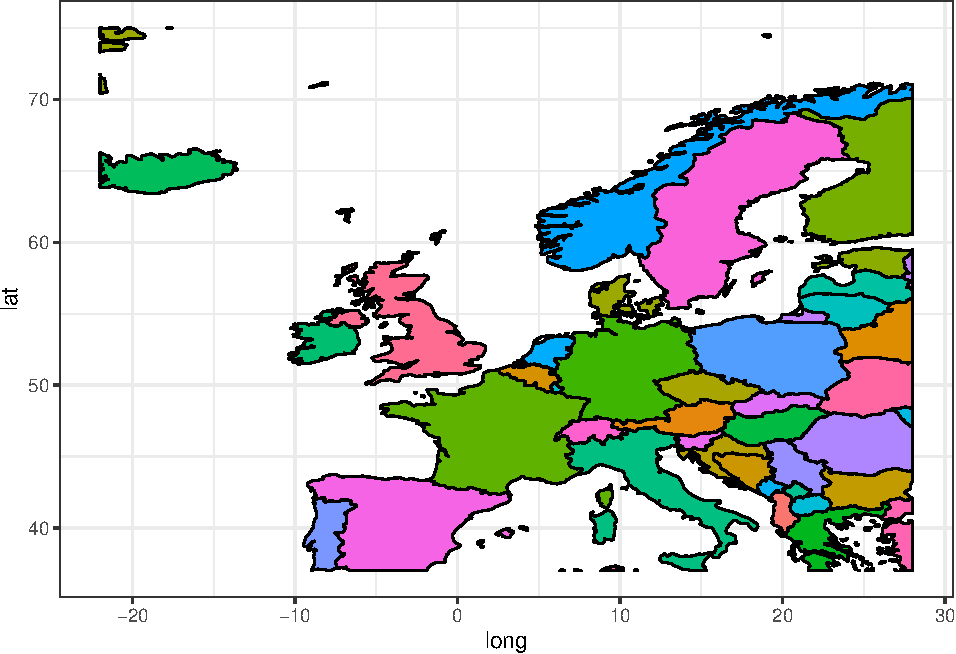
\includegraphics{esds_book_files/figure-latex/unnamed-chunk-34-1.pdf}

As we saw in the earlier plot of the tower locations only some countries in Europe contain towers. Therefore, we want to crop our map to include only those countries.

To do this we first make a vector which is a list of the country each tower is located in. We get this from \emph{df\_site\_country\_info}.
Then we filter out only those countries with a tower in them and voilà, plot the countries and tower locations as a result.

\begin{Shaded}
\begin{Highlighting}[]
\NormalTok{countries_with_site <-}\StringTok{ }\NormalTok{df_sites_country_info }\OperatorTok\StringTok{ }\KeywordTok{pull}\NormalTok{(SOVEREIGNT) }\OperatorTok\StringTok{ }\KeywordTok{as.character}\NormalTok{()}

\CommentTok{# resulting character vector (without NAs)}
\NormalTok{countries_with_site }\OperatorTok\StringTok{ }\KeywordTok{na.omit}\NormalTok{()}
\end{Highlighting}
\end{Shaded}

\begin{verbatim}
##  [1] "Belgium"     "Belgium"     "Belgium"     "Switzerland" "Switzerland"
##  [6] "Switzerland" "Switzerland" "Switzerland" "Switzerland" "Germany"    
## [11] "Germany"     "Germany"     "Germany"     "Germany"     "Denmark"    
## [16] "Finland"     "Finland"     "France"      "France"      "France"     
## [21] "France"      "Italy"       "Italy"       "Italy"       "Italy"      
## [26] "Italy"       "Italy"       "Italy"       "Italy"       "Italy"      
## [31] "Netherlands" "Czechia"    
## attr(,"na.action")
## [1] 33
## attr(,"class")
## [1] "omit"
\end{verbatim}

\begin{Shaded}
\begin{Highlighting}[]
\CommentTok{# country with towers filtered}
\NormalTok{shp_df_sub <-}\StringTok{ }\NormalTok{shp_df }\OperatorTok\StringTok{ }
\StringTok{  }\KeywordTok{filter}\NormalTok{(id }\OperatorTok\StringTok{ }\NormalTok{countries_with_site)}

\CommentTok{# plot result}
\KeywordTok{ggplot}\NormalTok{() }\OperatorTok{+}\StringTok{ }
\StringTok{  }\KeywordTok{geom_polygon}\NormalTok{(}\DataTypeTok{data =}\NormalTok{ shp_df_sub, }\KeywordTok{aes}\NormalTok{(}\DataTypeTok{x =}\NormalTok{ long, }\DataTypeTok{y =}\NormalTok{ lat, }\DataTypeTok{group =}\NormalTok{ group, }\DataTypeTok{fill =}\NormalTok{ id), }\DataTypeTok{colour =} \StringTok{"black"}\NormalTok{) }\OperatorTok{+}
\StringTok{  }\KeywordTok{geom_point}\NormalTok{(}\DataTypeTok{data =}\NormalTok{ df_sites, }\KeywordTok{aes}\NormalTok{(}\DataTypeTok{x =}\NormalTok{ lon, }\DataTypeTok{y =}\NormalTok{ lat)) }\OperatorTok{+}
\StringTok{  }\KeywordTok{theme_bw}\NormalTok{()}
\end{Highlighting}
\end{Shaded}

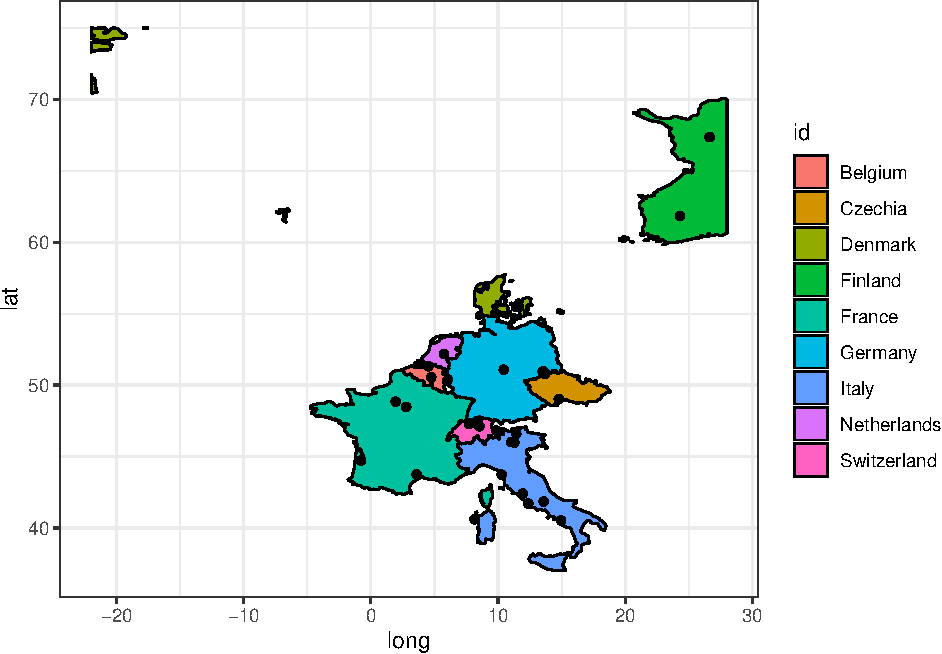
\includegraphics{esds_book_files/figure-latex/unnamed-chunk-35-1.pdf}

\textbf{Checkpoint}

You just learnt how to plot \emph{europe\_shape} coloured by country (``SOVREIGNT''), now plot it coloured by region in europe.
Start by finding the column that gives you this information in \texttt{europe\_shape@data}.

\textbf{Solution}

\begin{Shaded}
\begin{Highlighting}[]
\CommentTok{# take a look at the column names}
\KeywordTok{names}\NormalTok{(europe_shape}\OperatorTok{@}\NormalTok{data)}
\end{Highlighting}
\end{Shaded}

\begin{verbatim}
##  [1] "featurecla" "scalerank"  "LABELRANK"  "SOVEREIGNT" "SOV_A3"    
##  [6] "ADM0_DIF"   "LEVEL"      "TYPE"       "ADMIN"      "ADM0_A3"   
## [11] "GEOU_DIF"   "GEOUNIT"    "GU_A3"      "SU_DIF"     "SUBUNIT"   
## [16] "SU_A3"      "BRK_DIFF"   "NAME"       "NAME_LONG"  "BRK_A3"    
## [21] "BRK_NAME"   "BRK_GROUP"  "ABBREV"     "POSTAL"     "FORMAL_EN" 
## [26] "FORMAL_FR"  "NAME_CIAWF" "NOTE_ADM0"  "NOTE_BRK"   "NAME_SORT" 
## [31] "NAME_ALT"   "MAPCOLOR7"  "MAPCOLOR8"  "MAPCOLOR9"  "MAPCOLOR13"
## [36] "POP_EST"    "POP_RANK"   "GDP_MD_EST" "POP_YEAR"   "LASTCENSUS"
## [41] "GDP_YEAR"   "ECONOMY"    "INCOME_GRP" "WIKIPEDIA"  "FIPS_10_"  
## [46] "ISO_A2"     "ISO_A3"     "ISO_A3_EH"  "ISO_N3"     "UN_A3"     
## [51] "WB_A2"      "WB_A3"      "WOE_ID"     "WOE_ID_EH"  "WOE_NOTE"  
## [56] "ADM0_A3_IS" "ADM0_A3_US" "ADM0_A3_UN" "ADM0_A3_WB" "CONTINENT" 
## [61] "REGION_UN"  "SUBREGION"  "REGION_WB"  "NAME_LEN"   "LONG_LEN"  
## [66] "ABBREV_LEN" "TINY"       "HOMEPART"   "MIN_ZOOM"   "MIN_LABEL" 
## [71] "MAX_LABEL"  "NE_ID"      "WIKIDATAID" "NAME_AR"    "NAME_BN"   
## [76] "NAME_DE"    "NAME_EN"    "NAME_ES"    "NAME_FR"    "NAME_EL"   
## [81] "NAME_HI"    "NAME_HU"    "NAME_ID"    "NAME_IT"    "NAME_JA"   
## [86] "NAME_KO"    "NAME_NL"    "NAME_PL"    "NAME_PT"    "NAME_RU"   
## [91] "NAME_SV"    "NAME_TR"    "NAME_VI"    "NAME_ZH"
\end{verbatim}

\begin{Shaded}
\begin{Highlighting}[]
\CommentTok{# make a df of the data needed from europe_shape}
\NormalTok{shp_df_region <-}\StringTok{ }\NormalTok{broom}\OperatorTok{::}\KeywordTok{tidy}\NormalTok{(europe_shape, }\DataTypeTok{region =} \StringTok{"SUBREGION"}\NormalTok{)}
\KeywordTok{head}\NormalTok{(shp_df_region)}
\end{Highlighting}
\end{Shaded}

\begin{verbatim}
## # A tibble: 6 x 7
##    long   lat order hole  piece group            id            
##   <dbl> <dbl> <int> <lgl> <fct> <fct>            <chr>         
## 1  28    42.0     1 FALSE 1     Eastern Europe.1 Eastern Europe
## 2  27.9  42.0     2 FALSE 1     Eastern Europe.1 Eastern Europe
## 3  27.8  42.0     3 FALSE 1     Eastern Europe.1 Eastern Europe
## 4  27.8  42.0     4 FALSE 1     Eastern Europe.1 Eastern Europe
## 5  27.7  42.0     5 FALSE 1     Eastern Europe.1 Eastern Europe
## 6  27.7  42.0     6 FALSE 1     Eastern Europe.1 Eastern Europe
\end{verbatim}

\begin{Shaded}
\begin{Highlighting}[]
\CommentTok{# plot europe coloured by region}
\KeywordTok{ggplot}\NormalTok{() }\OperatorTok{+}\StringTok{ }
\StringTok{  }\KeywordTok{geom_polygon}\NormalTok{(}\DataTypeTok{data =}\NormalTok{ shp_df_region, }\KeywordTok{aes}\NormalTok{(}\DataTypeTok{x =}\NormalTok{ long, }\DataTypeTok{y =}\NormalTok{ lat, }\DataTypeTok{group =}\NormalTok{ group, }\DataTypeTok{fill =}\NormalTok{ id), }\DataTypeTok{colour =} \StringTok{"black"}\NormalTok{) }\OperatorTok{+}
\StringTok{  }\KeywordTok{geom_point}\NormalTok{(}\DataTypeTok{data =}\NormalTok{ df_sites, }\KeywordTok{aes}\NormalTok{(}\DataTypeTok{x =}\NormalTok{ lon, }\DataTypeTok{y =}\NormalTok{ lat)) }\OperatorTok{+}
\StringTok{  }\KeywordTok{theme_bw}\NormalTok{()}
\end{Highlighting}
\end{Shaded}

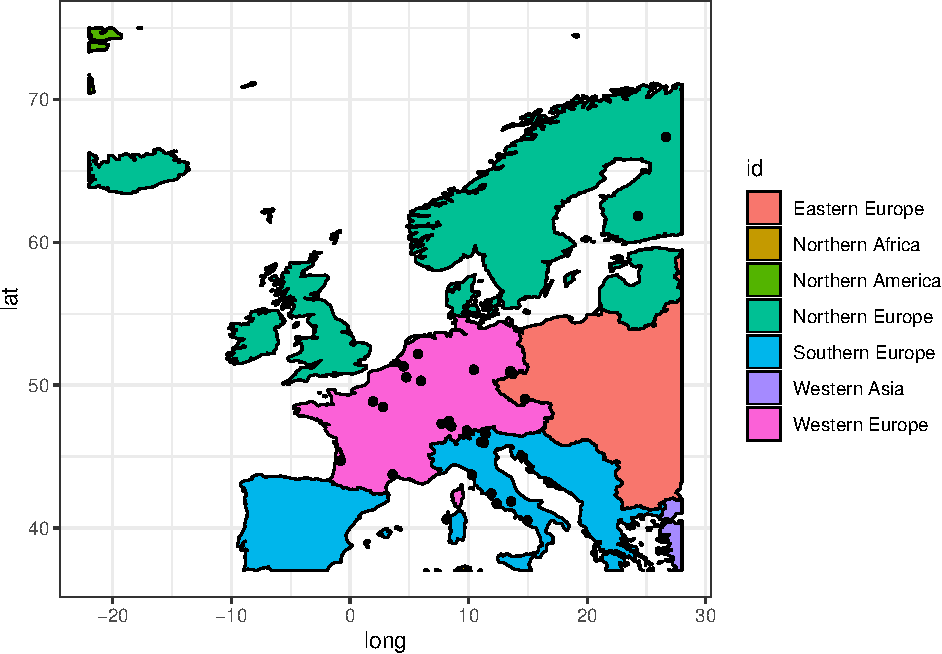
\includegraphics{esds_book_files/figure-latex/unnamed-chunk-36-1.pdf}

\hypertarget{rasters}{%
\subsection{Rasters}\label{rasters}}

Next up are rasters. A raster is a matrix or grid of cells each of which contains information in the form of a value.

A raster object consists primarily of:

\begin{itemize}
\tightlist
\item
  A grid of cells;\\
\item
  A coordinate reference system (CRS) for the grid and its cells so that we know the location to which the grid refers;
\item
  A variable of interest for which each cell in the grid has a value, and;
\item
  Other information relating to the CRS, projection, resolution, etc.
\end{itemize}

Let's take a look at some rasters and get familiar with some functions to analyse them.

Since our goal ultimate goal is to predict productivity, we will consider different factors that might explain productivity, for example, landcover and temperature.
To start off we'll look at some landcover data. With this data, we can investigate the surroundings of the Fluxnet towers. This data gives us the different classes of physical coverage of the Earth's surface, such as forests, grasslands, croplands, lakes, etc. Landcover types affect fluxes measured by the tower through the vegetation that characterizes them, or by influencing the radiation budget through albedo, or water availability. Although we have some information from the overview file of the towers, we can still check whether we can confirm this information. We will load landcover data from GlobCover provided by the \href{http://due.esrin.esa.int/page_globcover.php}{European space agency (ESA)}. This project provides landcover maps observations of surface reflectance from the 300m MERIS sensor on board the ENVISAT satellite mission as their input.

\begin{Shaded}
\begin{Highlighting}[]
\CommentTok{# library(raster) -> we have already done this but remember you need this to load rasters!}

\NormalTok{raster_landcover <-}\StringTok{ }\KeywordTok{raster}\NormalTok{(}\StringTok{"./data/Globcover_EU.tif"}\NormalTok{)}
\end{Highlighting}
\end{Shaded}

This landcover data consists of different categories, these GlobCover categories are based on the Land Cover Classification System (LCCS) which was
developed by the Food and Agricultural Organization of the United Nations (FAO) to provide a consistent framework for the classification of mapping land cover. They include various types of forest, shrub- and grasslands, cropland and artificial surfaces.

Before we look at the data, we first reduce the spatial extent that the raster covers. We crop it to a rectangle around the site location of CH-Lae (+/- 2 degrees in longitudinal direction, +/- 1 degree in latitudinal direction).

\begin{Shaded}
\begin{Highlighting}[]
\NormalTok{bounding_box <-}\StringTok{ }\KeywordTok{extent}\NormalTok{(lon_lae}\DecValTok{-2}\NormalTok{, lon_lae}\OperatorTok{+}\DecValTok{2}\NormalTok{, lat_lae}\DecValTok{-1}\NormalTok{, lat_lae}\OperatorTok{+}\DecValTok{1}\NormalTok{)}
\NormalTok{raster_landcover_crop <-}\StringTok{ }\KeywordTok{crop}\NormalTok{(raster_landcover, bounding_box)}
\end{Highlighting}
\end{Shaded}

We can plot our raster as the region around our tower. To indicate the position of our tower, we add a red dot.

\begin{Shaded}
\begin{Highlighting}[]
\KeywordTok{plot}\NormalTok{(raster_landcover_crop, }\DataTypeTok{legend=}\OtherTok{FALSE}\NormalTok{, }\DataTypeTok{xlab=}\StringTok{"longitude"}\NormalTok{, }\DataTypeTok{ylab=}\StringTok{"latitude"}\NormalTok{)}
\end{Highlighting}
\end{Shaded}


\includegraphics{esds_book_files/figure-latex/unnamed-chunk-39-1.pdf}

\begin{verbatim}
## Warning in plot.window(...): "legend" is not a graphical parameter
\end{verbatim}

\begin{verbatim}
## Warning in plot.xy(xy, type, ...): "legend" is not a graphical parameter
\end{verbatim}

\begin{verbatim}
## Warning in title(...): "legend" is not a graphical parameter
\end{verbatim}

\begin{verbatim}
## Warning in graphics::rasterImage(z, bb[1], bb[3], bb[2], bb[4], interpolate =
## interpolate, : "legend" is not a graphical parameter
\end{verbatim}

\begin{Shaded}
\begin{Highlighting}[]
\KeywordTok{points}\NormalTok{(lon_lae, lat_lae, }\DataTypeTok{pch =} \DecValTok{16}\NormalTok{, }\DataTypeTok{col =} \StringTok{"red"}\NormalTok{)}
\end{Highlighting}
\end{Shaded}

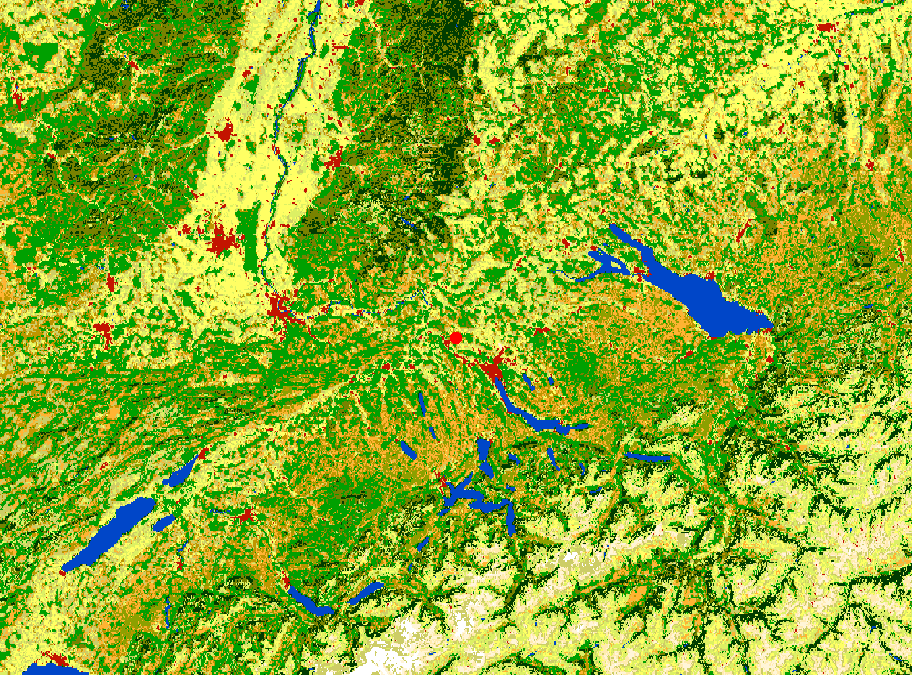
\includegraphics{esds_book_files/figure-latex/unnamed-chunk-39-2.pdf}

If we want to conduct analysis using two different rasters, we have to make sure they have the same resolution and are aligned on the same grid. Let's read a second raster and compare the grids. We load spatio-temporal temperature rasters available from \href{https://chelsa-climate.org}{CHELSA} to complement our flux tower measurements for further analysis.
The temperature raster data from CHELSA provides free high-resolution climate data (temperature and precipitation) for the past and the future. The past data we use here are downscaled model output temperature and precipitation estimates of the ERA-Interim climatic reanalysis (forecast models and data assimilation systems reanalysing archived observations). While the temperature algorithm is based on statistical downscaling of atmospheric temperatures, the precipitation algorithm incorporates orographic predictors including wind fields, valley exposition, and boundary layer height, with subsequent bias correction. The data we use consists of a monthly temperature and precipitation time series over the area of Europe from 2006 to 2012 in January. To compare this new raster with the previous one we need to crop it to the same region as the tower.

\begin{Shaded}
\begin{Highlighting}[]
\NormalTok{raster_chelsa <-}\StringTok{ }\KeywordTok{raster}\NormalTok{(}\StringTok{"./data/Chelsa_t_mean_2006-2012.tif"}\NormalTok{)}
\NormalTok{raster_chelsa_crop <-}\StringTok{ }\KeywordTok{crop}\NormalTok{(raster_chelsa, bounding_box)}
\end{Highlighting}
\end{Shaded}

We now plot our raster.

\begin{Shaded}
\begin{Highlighting}[]
\NormalTok{pal <-}\StringTok{ }\KeywordTok{colorRampPalette}\NormalTok{(}\KeywordTok{c}\NormalTok{(}\StringTok{"purple"}\NormalTok{,}\StringTok{"blue"}\NormalTok{,}\StringTok{"cyan"}\NormalTok{,}\StringTok{"green"}\NormalTok{,}\StringTok{"yellow"}\NormalTok{,}\StringTok{"red"}\NormalTok{))}
\KeywordTok{plot}\NormalTok{(raster_chelsa_crop, }\DataTypeTok{col =} \KeywordTok{pal}\NormalTok{(}\DecValTok{20}\NormalTok{), }\DataTypeTok{xlab=}\StringTok{"longitude"}\NormalTok{, }\DataTypeTok{ylab=}\StringTok{"latitude"}\NormalTok{)}
\KeywordTok{points}\NormalTok{(lon_lae, lat_lae, }\DataTypeTok{pch =} \DecValTok{16}\NormalTok{, }\DataTypeTok{col =} \StringTok{"red"}\NormalTok{)}
\end{Highlighting}
\end{Shaded}

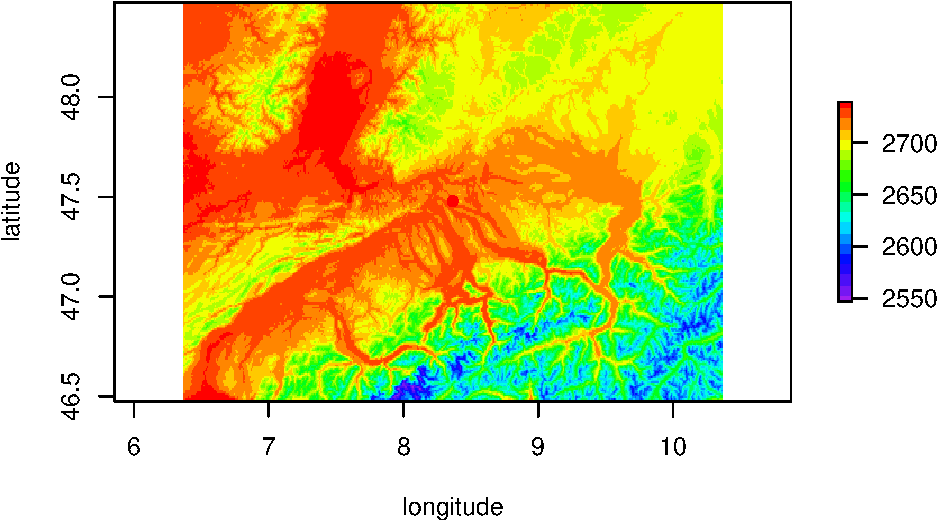
\includegraphics{esds_book_files/figure-latex/unnamed-chunk-41-1.pdf}

We see that the temperature units are not in a comprehensive format. To change the unit from Kelvin x10 to degree Celsius we have to divide the data by 10 and subtract 273.15.

\begin{Shaded}
\begin{Highlighting}[]
\NormalTok{raster_chelsa_crop <-}\StringTok{ }\NormalTok{raster_chelsa_crop}\OperatorTok{/}\DecValTok{10}\FloatTok{-273.15}
\end{Highlighting}
\end{Shaded}

We plot our raster again.

\begin{Shaded}
\begin{Highlighting}[]
\NormalTok{pal <-}\StringTok{ }\KeywordTok{colorRampPalette}\NormalTok{(}\KeywordTok{c}\NormalTok{(}\StringTok{"purple"}\NormalTok{,}\StringTok{"blue"}\NormalTok{,}\StringTok{"cyan"}\NormalTok{,}\StringTok{"green"}\NormalTok{,}\StringTok{"yellow"}\NormalTok{,}\StringTok{"red"}\NormalTok{))}
\KeywordTok{plot}\NormalTok{(raster_chelsa_crop, }\DataTypeTok{col =} \KeywordTok{pal}\NormalTok{(}\DecValTok{20}\NormalTok{), }\DataTypeTok{xlab=}\StringTok{"longitude"}\NormalTok{, }\DataTypeTok{ylab=}\StringTok{"latitude"}\NormalTok{)}
\KeywordTok{points}\NormalTok{(lon_lae, lat_lae, }\DataTypeTok{pch =} \DecValTok{16}\NormalTok{, }\DataTypeTok{col =} \StringTok{"red"}\NormalTok{)}
\end{Highlighting}
\end{Shaded}

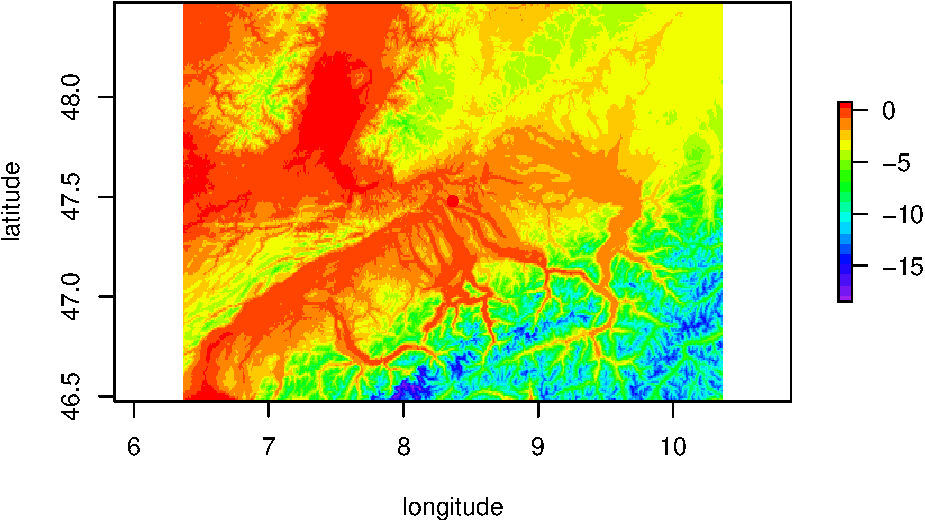
\includegraphics{esds_book_files/figure-latex/unnamed-chunk-43-1.pdf}

We have seen some of the basic functions in the package \texttt{raster}. Now we will load one more package to work with raster files. We use the package \texttt{rasterVis}. This package contains methods for enhanced visualization and interaction with raster data. It implements visualization methods for quantitative data and categorical data, both for univariate and multivariate rasters. It also provides methods to display spatiotemporal rasters, and vector fields.

\begin{Shaded}
\begin{Highlighting}[]
\KeywordTok{library}\NormalTok{(rasterVis)}
\KeywordTok{library}\NormalTok{(RColorBrewer)}

\NormalTok{mapTheme <-}\StringTok{ }\KeywordTok{rasterTheme}\NormalTok{(}\DataTypeTok{region =} \KeywordTok{rev}\NormalTok{(}\KeywordTok{brewer.pal}\NormalTok{(}\DecValTok{8}\NormalTok{,}\StringTok{"RdYlBu"}\NormalTok{)))}
\NormalTok{plt <-}\StringTok{ }\KeywordTok{levelplot}\NormalTok{(raster_chelsa_crop, }\DataTypeTok{margin=}\OtherTok{FALSE}\NormalTok{, }\DataTypeTok{par.settings =}\NormalTok{ mapTheme)}
\NormalTok{plt}
\end{Highlighting}
\end{Shaded}

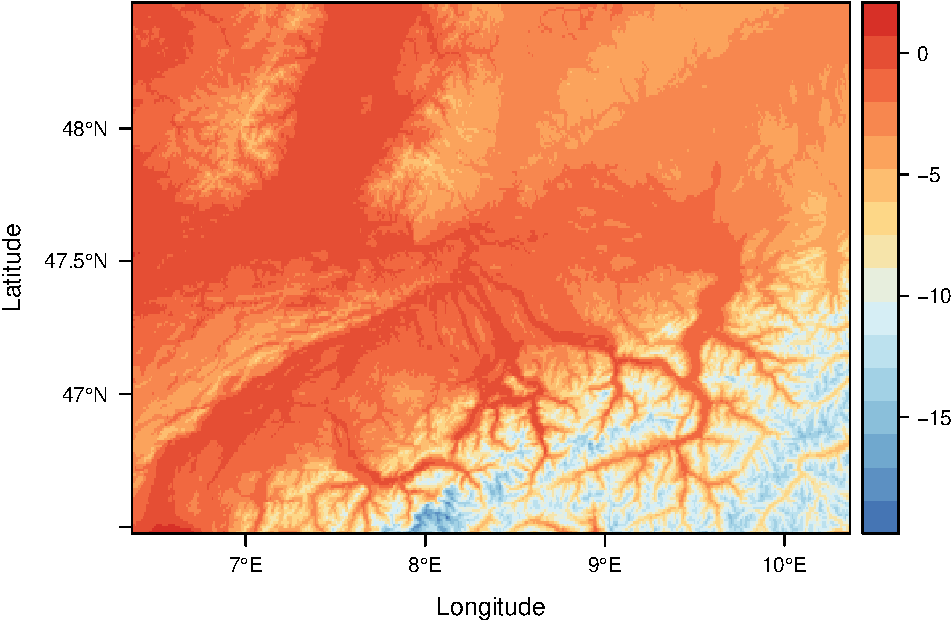
\includegraphics{esds_book_files/figure-latex/unnamed-chunk-44-1.pdf}

\textbf{Checkpoint}

Create your own small raster with 100 grid cells. Give it values, a projection (e.g.~`+proj=utm +zone=48 +datum=WGS84') and plot it.

\emph{Bonus}: If you chose the example projection provided, add \emph{europe\_shape} to your plot.

\textbf{Solution}

\begin{Shaded}
\begin{Highlighting}[]
\CommentTok{# create a raster}
\CommentTok{# short compact version}
\NormalTok{myraster <-}\StringTok{ }\KeywordTok{raster}\NormalTok{(}\DataTypeTok{ncol=}\DecValTok{10}\NormalTok{, }\DataTypeTok{nrow=}\DecValTok{10}\NormalTok{)}
\CommentTok{# OR }
\CommentTok{# longer version}
\NormalTok{myraster <-}\StringTok{ }\KeywordTok{raster}\NormalTok{()}
\KeywordTok{ncol}\NormalTok{(myraster) <-}\StringTok{ }\DecValTok{10}
\KeywordTok{nrow}\NormalTok{(myraster) <-}\StringTok{ }\DecValTok{10}

\CommentTok{# add values to the raster, this can be done in many ways here are two examples:}
\KeywordTok{values}\NormalTok{(myraster) <-}\StringTok{ }\DecValTok{1}\OperatorTok{:}\KeywordTok{ncell}\NormalTok{(myraster)}
\CommentTok{# OR }
\KeywordTok{values}\NormalTok{(myraster) <-}\StringTok{ }\KeywordTok{runif}\NormalTok{(}\KeywordTok{ncell}\NormalTok{(myraster))}

\CommentTok{# add a projection}
\KeywordTok{projection}\NormalTok{(myraster) <-}\StringTok{ "+proj=utm +zone=48 +datum=WGS84"}

\CommentTok{# plot it}
\KeywordTok{plot}\NormalTok{(myraster)}
\CommentTok{# for fun let's see where europe would be on our raster, since it has a projection...}
\KeywordTok{plot}\NormalTok{(europe_shape, }\DataTypeTok{add=}\OtherTok{TRUE}\NormalTok{)}
\end{Highlighting}
\end{Shaded}

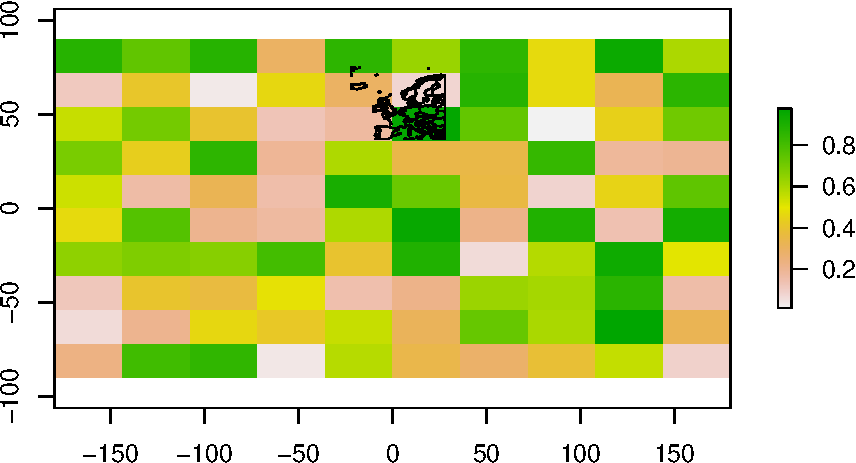
\includegraphics{esds_book_files/figure-latex/unnamed-chunk-45-1.pdf}

\hypertarget{aggregating}{%
\subsubsection{Aggregating}\label{aggregating}}

A \textbf{raster grid} is uniquely defined by an \emph{origin}, a point that one of the intersections of grid lines, and its resolution, the magnitude of each cell-side. In the R package \texttt{raster}, the origin is defined as the point closest to (0,0) that is still an intersection of grid lines. The functions \texttt{origin()} and \texttt{res()} from the R package \texttt{raster} return the origin and resolution of a raster object. So let's see what the resolution and origin of the rasters we loaded before are.

\begin{Shaded}
\begin{Highlighting}[]
\KeywordTok{res}\NormalTok{(raster_landcover)}
\end{Highlighting}
\end{Shaded}

\begin{verbatim}
## [1] 0.002777778 0.002777778
\end{verbatim}

\begin{Shaded}
\begin{Highlighting}[]
\KeywordTok{res}\NormalTok{(raster_chelsa)}
\end{Highlighting}
\end{Shaded}

\begin{verbatim}
## [1] 0.008333333 0.008333333
\end{verbatim}

\begin{Shaded}
\begin{Highlighting}[]
\KeywordTok{origin}\NormalTok{(raster_landcover)}
\end{Highlighting}
\end{Shaded}

\begin{verbatim}
## [1]  0.001388889 -0.001388889
\end{verbatim}

\begin{Shaded}
\begin{Highlighting}[]
\KeywordTok{origin}\NormalTok{(raster_chelsa)}
\end{Highlighting}
\end{Shaded}

\begin{verbatim}
## [1] -0.000139609 -0.000139249
\end{verbatim}

Landcover has a much higher resolution. Let's re-grid the Landcover raster to match the grid of the Chelsa raster. Aggregating means resampling an input raster to a coarser resolution based on a specified aggregation strategy. We now determine the aggregation factor by dividing the resolution of the landcover raster by that of the Chelsa raster. We do it both for the longitude and latitude to make sure they match.

\begin{Shaded}
\begin{Highlighting}[]
\NormalTok{res_landcover <-}\StringTok{ }\KeywordTok{res}\NormalTok{(raster_landcover)}
\NormalTok{res_chelsa <-}\StringTok{ }\KeywordTok{res}\NormalTok{(raster_chelsa)}
\NormalTok{factor_agg_lon <-}\StringTok{ }\NormalTok{res_chelsa[}\DecValTok{1}\NormalTok{] }\OperatorTok{/}\StringTok{ }\NormalTok{res_landcover[}\DecValTok{1}\NormalTok{]}
\NormalTok{factor_agg_lat <-}\StringTok{ }\NormalTok{res_chelsa[}\DecValTok{2}\NormalTok{] }\OperatorTok{/}\StringTok{ }\NormalTok{res_landcover[}\DecValTok{2}\NormalTok{]}
\KeywordTok{print}\NormalTok{(factor_agg_lon); }\KeywordTok{print}\NormalTok{(factor_agg_lat)}
\end{Highlighting}
\end{Shaded}

\begin{verbatim}
## [1] 3
\end{verbatim}

\begin{verbatim}
## [1] 3
\end{verbatim}

First, we observed that the land cover raster has a higher resolution than the temperature raster, now we now it is 3 times higher. So we need to transform the landcover raster to make sure it has the same grid (same \emph{origin} and \emph{resolution}) as the temperature raster. This will allow us to combine them in a potential analysis. We achieve this using \texttt{aggregate()} from the R package \texttt{raster} to obtain a sum of edges raster at 1000m x 1000m resolution.

The aggregate function takes three main arguments.
* \textbf{\emph{x}} : the raster object to aggregate,
* \textbf{\emph{fact}} : aggregation factor, i.e.~the number of current cells that will make up the side of one of the new cells, and,
* \textbf{\emph{fun}} : the function to apply to summarize the raster values of the fact\^{}2 (in this case 3ˆ2=9) cells.

We aggregate the landcover raster at 1km using the aggregation factor calculated above.

\begin{Shaded}
\begin{Highlighting}[]
\NormalTok{raster_landcover_crop_agg <-}\StringTok{ }\KeywordTok{aggregate}\NormalTok{(raster_landcover_crop, }\DataTypeTok{fact =}\NormalTok{ factor_agg_lon, }\DataTypeTok{fun =}\NormalTok{ modal)}
\end{Highlighting}
\end{Shaded}

We check the resolutions and origin of the two rasters and plot our the new landcover one.

\begin{Shaded}
\begin{Highlighting}[]
\KeywordTok{res}\NormalTok{(raster_landcover_crop_agg)}
\end{Highlighting}
\end{Shaded}

\begin{verbatim}
## [1] 0.008333333 0.008333333
\end{verbatim}

\begin{Shaded}
\begin{Highlighting}[]
\KeywordTok{res}\NormalTok{(raster_chelsa)}
\end{Highlighting}
\end{Shaded}

\begin{verbatim}
## [1] 0.008333333 0.008333333
\end{verbatim}

\begin{Shaded}
\begin{Highlighting}[]
\KeywordTok{origin}\NormalTok{(raster_landcover_crop_agg)}
\end{Highlighting}
\end{Shaded}

\begin{verbatim}
## [1] -0.001388889 -0.004166667
\end{verbatim}

\begin{Shaded}
\begin{Highlighting}[]
\KeywordTok{origin}\NormalTok{(raster_chelsa)}
\end{Highlighting}
\end{Shaded}

\begin{verbatim}
## [1] -0.000139609 -0.000139249
\end{verbatim}

\begin{Shaded}
\begin{Highlighting}[]
\KeywordTok{plot}\NormalTok{(raster_landcover_crop_agg, }\DataTypeTok{legend=}\OtherTok{FALSE}\NormalTok{, }\DataTypeTok{xlab=}\StringTok{"longitude"}\NormalTok{, }\DataTypeTok{ylab=}\StringTok{"latitude"}\NormalTok{)}
\end{Highlighting}
\end{Shaded}

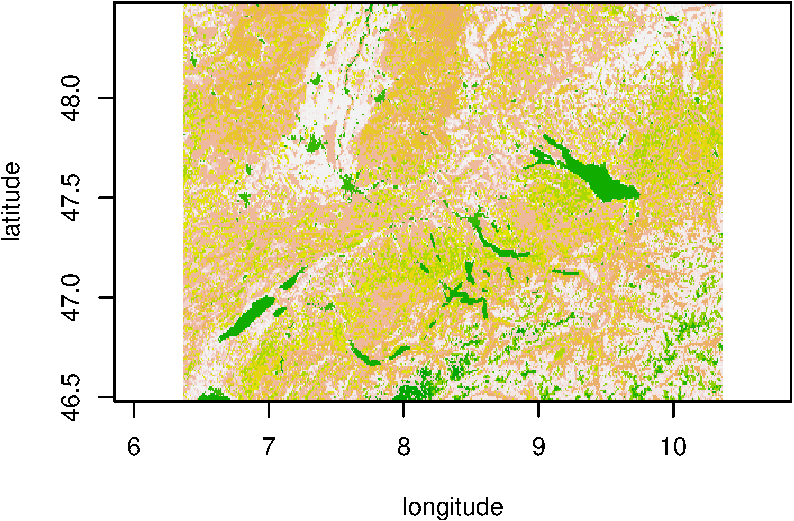
\includegraphics{esds_book_files/figure-latex/unnamed-chunk-50-1.pdf}

We can see that the resolutions are now the same but the origin still differs. To get matching origins we must do another step: align the rasters.

\hypertarget{aligning}{%
\subsubsection{Aligning}\label{aligning}}

Aligning rasters is done using the function \texttt{resample()}. There are two main resampling methods: \emph{Nearest Neighbour} or \emph{Bilinear Interpolation}, which method is used depends upon the input data and its use after the operation is performed.

\textbf{\emph{Nearest Neighbour}} is best used for categorical data like land-use classification or slope classification. The values that go into the grid stay exactly the same, a 2 comes out as a 2, and 99 comes out as 99. The value of the output cell is determined by the nearest cell center on the input grid. Nearest Neighbor can be used on continuous data but the results can be blocky.

\textbf{\emph{Bilinear Interpolation}} uses a weighted average of the four nearest cell centers. The closer an input cell center is to the output cell center, the higher the influence of its value is on the output cell value. This means that the output value could be different than the nearest input, but is always within the same range of values as the input. Since the values can change, Bilinear is not recommended for categorical data. Instead, it should be used for continuous data like elevation and raw slope values.

\begin{Shaded}
\begin{Highlighting}[]
\NormalTok{raster_landcover_crop_resampl <-}\StringTok{ }\KeywordTok{resample}\NormalTok{(raster_landcover_crop, raster_chelsa_crop, }\DataTypeTok{method=}\StringTok{"ngb"}\NormalTok{)}
\KeywordTok{plot}\NormalTok{(raster_landcover_crop_resampl, }\DataTypeTok{legend=}\OtherTok{FALSE}\NormalTok{, }\DataTypeTok{xlab=}\StringTok{"longitude"}\NormalTok{, }\DataTypeTok{ylab=}\StringTok{"latitude"}\NormalTok{)}
\end{Highlighting}
\end{Shaded}


\includegraphics{esds_book_files/figure-latex/unnamed-chunk-51-1.pdf}

\begin{verbatim}
## Warning in plot.window(...): "legend" is not a graphical parameter
\end{verbatim}

\begin{verbatim}
## Warning in plot.xy(xy, type, ...): "legend" is not a graphical parameter
\end{verbatim}

\begin{verbatim}
## Warning in title(...): "legend" is not a graphical parameter
\end{verbatim}

\begin{verbatim}
## Warning in graphics::rasterImage(z, bb[1], bb[3], bb[2], bb[4], interpolate =
## interpolate, : "legend" is not a graphical parameter
\end{verbatim}

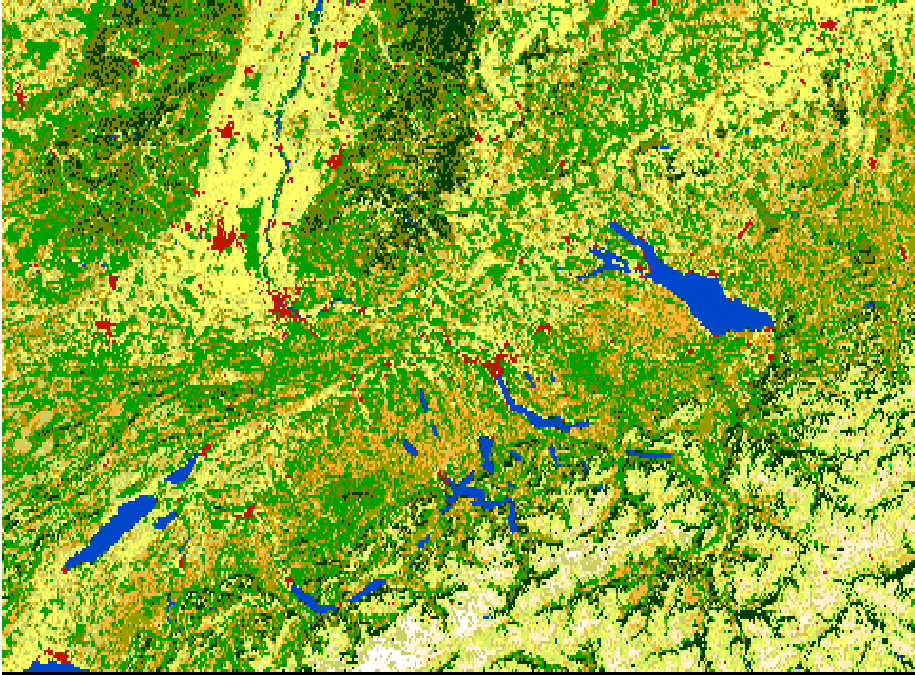
\includegraphics{esds_book_files/figure-latex/unnamed-chunk-51-2.pdf}

Now we check if the two rasters are aligned.

\begin{Shaded}
\begin{Highlighting}[]
\KeywordTok{res}\NormalTok{(raster_landcover_crop_resampl)}
\end{Highlighting}
\end{Shaded}

\begin{verbatim}
## [1] 0.008333333 0.008333333
\end{verbatim}

\begin{Shaded}
\begin{Highlighting}[]
\KeywordTok{res}\NormalTok{(raster_chelsa)}
\end{Highlighting}
\end{Shaded}

\begin{verbatim}
## [1] 0.008333333 0.008333333
\end{verbatim}

\begin{Shaded}
\begin{Highlighting}[]
\KeywordTok{origin}\NormalTok{(raster_landcover_crop_resampl)}
\end{Highlighting}
\end{Shaded}

\begin{verbatim}
## [1] -0.000139609 -0.000139249
\end{verbatim}

\begin{Shaded}
\begin{Highlighting}[]
\KeywordTok{origin}\NormalTok{(raster_chelsa)}
\end{Highlighting}
\end{Shaded}

\begin{verbatim}
## [1] -0.000139609 -0.000139249
\end{verbatim}

Now the two rasters are aligned.

\hypertarget{point-extraction}{%
\subsubsection{Point extraction}\label{point-extraction}}

In this section, we will show you how to extract data from our rasters or spatial data. We will be extracting the values for the locations of our towers. The function to extract values is aptly named \texttt{extract()}. First, we specify the raster from which the values should be extracted and then the exact sites at which the values should be extracted. Here, we combine all this into a neat dataframe.

\begin{Shaded}
\begin{Highlighting}[]
\NormalTok{df_sites_temp <-}\StringTok{ }\KeywordTok{read_csv}\NormalTok{(}\StringTok{"./data/fluxnet_site_info_reduced.csv"}\NormalTok{)}

\NormalTok{df_sites_temp <-}\StringTok{ }\KeywordTok{extract}\NormalTok{(raster_chelsa, sp_sites, }\DataTypeTok{sp =} \OtherTok{TRUE}\NormalTok{) }\OperatorTok\StringTok{ }
\StringTok{  }\KeywordTok{as_tibble}\NormalTok{() }\OperatorTok\StringTok{ }
\StringTok{  }\KeywordTok{right_join}\NormalTok{(df_sites_temp, }\DataTypeTok{by =} \KeywordTok{c}\NormalTok{(}\StringTok{"lon"}\NormalTok{, }\StringTok{"lat"}\NormalTok{)) }\OperatorTok\StringTok{ }
\StringTok{  }\NormalTok{dplyr}\OperatorTok{::}\KeywordTok{rename}\NormalTok{(}\DataTypeTok{temp_chelsa =}\NormalTok{ Chelsa_t_mean_}\FloatTok{2006.2012}\NormalTok{)}
\end{Highlighting}
\end{Shaded}

In the lectures, you have already, heard that we must always be aware of modelled data and be aware of its limitations. Therefore, we don't just want to use CHELSA temperature data. It is important to consider different models and compare them. Hence, we'll look at another climate model. We load and plot the provided rasters showing the mean annual temperatures for the Worldclim data for the years 2006-2012. WorldClim is a set of global climate layers (gridded climate data) with a spatial resolution of about 1 km2. We extract values from Worldclim at the same tower sites and add them to the \emph{df\_sites} data frame. Now we have a tidy dataframe with the site, latitude and longitude, temperatures for Chelsa and WorldClim at each tower location.

\begin{Shaded}
\begin{Highlighting}[]
\NormalTok{raster_worldclim <-}\StringTok{ }\KeywordTok{raster}\NormalTok{(}\StringTok{"./data/WC_mean_t_2006-2012.tif"}\NormalTok{)}

\NormalTok{df_sites_temp <-}\StringTok{ }\KeywordTok{extract}\NormalTok{(raster_worldclim, sp_sites, }\DataTypeTok{sp =} \OtherTok{TRUE}\NormalTok{) }\OperatorTok\StringTok{ }
\StringTok{  }\KeywordTok{as_tibble}\NormalTok{() }\OperatorTok\StringTok{ }
\StringTok{  }\KeywordTok{right_join}\NormalTok{(df_sites_temp, }\DataTypeTok{by =} \KeywordTok{c}\NormalTok{(}\StringTok{"lon"}\NormalTok{, }\StringTok{"lat"}\NormalTok{)) }\OperatorTok\StringTok{ }
\StringTok{  }\NormalTok{dplyr}\OperatorTok{::}\KeywordTok{rename}\NormalTok{(}\DataTypeTok{temp_wc =}\NormalTok{ WC_mean_t_}\FloatTok{2006.2012}\NormalTok{)}

\KeywordTok{head}\NormalTok{(df_sites_temp)}
\end{Highlighting}
\end{Shaded}

\begin{verbatim}
## # A tibble: 6 x 5
##   temp_wc   lon   lat temp_chelsa site  
##     <dbl> <dbl> <dbl>       <dbl> <chr> 
## 1  -0.633  4.52  51.3        2750 BE-Bra
## 2  -1.45   4.75  50.6        2741 BE-Lon
## 3  -3.75   6.00  50.3        2716 BE-Vie
## 4  -4.76   8.41  47.2        2730 CH-Cha
## 5  -4.97   8.54  47.1        2699 CH-Fru
## 6  -5.38   8.36  47.5        2710 CH-Lae
\end{verbatim}

We get the monthly mean temperature of Jan 2006 from FLUXNET data.

\begin{Shaded}
\begin{Highlighting}[]
\KeywordTok{library}\NormalTok{(lubridate)}
\KeywordTok{load}\NormalTok{(}\StringTok{"./data/ddf_allsites_nested_joined.RData"}\NormalTok{)}

\NormalTok{df_sites_temp <-}\StringTok{ }\NormalTok{ddf_allsites_nested_joined }\OperatorTok\StringTok{ }
\StringTok{  }\NormalTok{dplyr}\OperatorTok{::}\KeywordTok{select}\NormalTok{(}\DataTypeTok{site =}\NormalTok{ siteid, data) }\OperatorTok\StringTok{ }
\StringTok{  }\KeywordTok{unnest}\NormalTok{(data) }\OperatorTok\StringTok{ }
\StringTok{  }\NormalTok{dplyr}\OperatorTok{::}\KeywordTok{select}\NormalTok{(site, TIMESTAMP, TA_F) }\OperatorTok\StringTok{ }
\StringTok{  }\KeywordTok{mutate}\NormalTok{(}\DataTypeTok{month =} \KeywordTok{month}\NormalTok{(TIMESTAMP), }\DataTypeTok{year =} \KeywordTok{year}\NormalTok{(TIMESTAMP)) }\OperatorTok\StringTok{ }
\StringTok{  }\KeywordTok{filter}\NormalTok{(month }\OperatorTok{==}\StringTok{ }\DecValTok{1}\NormalTok{, year }\OperatorTok{==}\StringTok{ }\DecValTok{2006}\NormalTok{) }\OperatorTok\StringTok{ }
\StringTok{  }\KeywordTok{group_by}\NormalTok{(site) }\OperatorTok\StringTok{ }
\StringTok{  }\KeywordTok{summarise}\NormalTok{(}\DataTypeTok{temp_fluxnet =} \KeywordTok{mean}\NormalTok{(TA_F)) }\OperatorTok\StringTok{ }
\StringTok{  }
\StringTok{  }\CommentTok{# add temp data extracted from spatial files (chelsa and worldclim)}
\StringTok{  }\KeywordTok{left_join}\NormalTok{(df_sites_temp, dplyr}\OperatorTok{::}\KeywordTok{select}\NormalTok{(site, temp_wc, temp_chelsa),}
            \DataTypeTok{by =} \StringTok{"site"}\NormalTok{)}
\end{Highlighting}
\end{Shaded}

We compare the climate models by showing the correlations with the tower's data. The dotted line shows what the linear model would look like if the values of our model and the tower data overlapped. The red line shows the actual linear model of the relationship between the climate model and the tower data. The closer the red line to the dotted line the better the model is at predicting the temperatures measured by the towers.

\begin{Shaded}
\begin{Highlighting}[]
\NormalTok{df_sites_temp}\OperatorTok{$}\NormalTok{temp_chelsa <-}\StringTok{ }\NormalTok{df_sites_temp}\OperatorTok{$}\NormalTok{temp_chelsa}\OperatorTok{/}\DecValTok{10} \FloatTok{-273.15}

\CommentTok{# we remove the sites we removed before}
\NormalTok{df_sites_temp <-}\StringTok{ }\NormalTok{df_sites_temp[}\OperatorTok{-}\KeywordTok{c}\NormalTok{(}\DecValTok{16}\NormalTok{, }\DecValTok{34}\NormalTok{), ]}

\NormalTok{df_sites_temp }\OperatorTok\StringTok{ }
\StringTok{  }\KeywordTok{ggplot}\NormalTok{(}\KeywordTok{aes}\NormalTok{(}\DataTypeTok{x =}\NormalTok{ temp_fluxnet, }\DataTypeTok{y =}\NormalTok{ temp_chelsa), }\DataTypeTok{xlim=}\KeywordTok{c}\NormalTok{(}\OperatorTok{-}\DecValTok{10}\NormalTok{,}\DecValTok{5}\NormalTok{)) }\OperatorTok{+}
\StringTok{  }\KeywordTok{geom_point}\NormalTok{() }\OperatorTok{+}
\StringTok{  }\KeywordTok{geom_abline}\NormalTok{(}\DataTypeTok{intercept=}\DecValTok{0}\NormalTok{, }\DataTypeTok{slope=}\DecValTok{1}\NormalTok{, }\DataTypeTok{linetype=}\StringTok{"dotted"}\NormalTok{) }\OperatorTok{+}
\StringTok{  }\KeywordTok{geom_smooth}\NormalTok{(}\DataTypeTok{method=}\StringTok{'lm'}\NormalTok{, }\DataTypeTok{color=}\StringTok{"red"}\NormalTok{, }\DataTypeTok{size=}\FloatTok{0.5}\NormalTok{, }\DataTypeTok{se=}\OtherTok{FALSE}\NormalTok{) }\OperatorTok{+}
\StringTok{  }\KeywordTok{theme_classic}\NormalTok{()}
\end{Highlighting}
\end{Shaded}

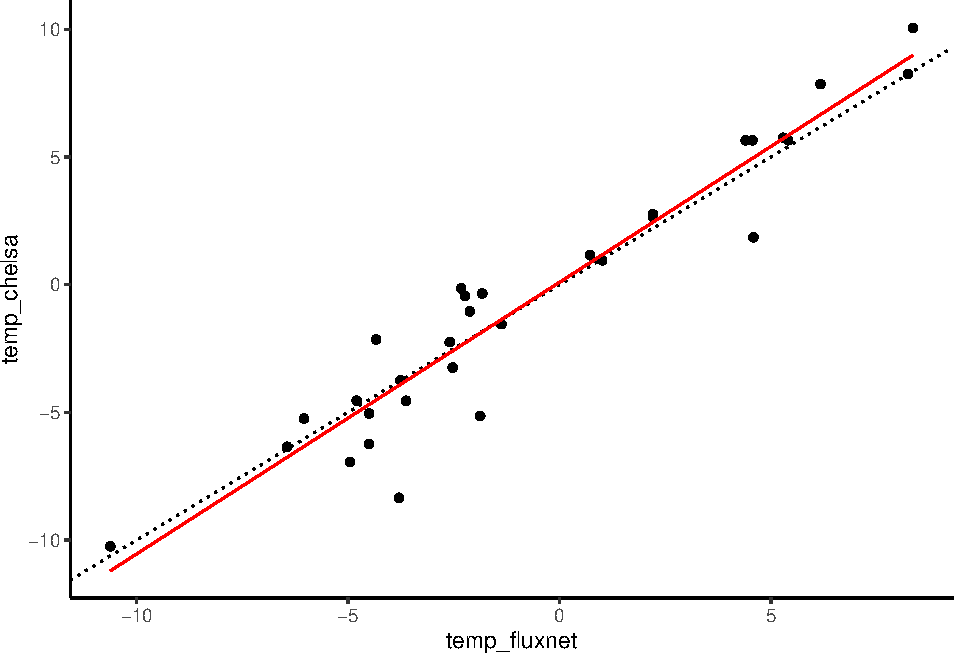
\includegraphics{esds_book_files/figure-latex/unnamed-chunk-56-1.pdf}

We compute the mean squared error (MSE). The MSE calculates the average of the squares of errors of all the data points from a fitted line or model. Put simply this is the difference between the data points (the actual data) and the estimated points given by the line or model. The values are squared to get positive values even if the difference is negative. Smaller values reflect less variation of the data. In a model you want to minimise the MSE, as this reflects that the model's predicted or estimated points are closer to your actual data.

\begin{Shaded}
\begin{Highlighting}[]
\KeywordTok{library}\NormalTok{(Metrics)}
\KeywordTok{mse}\NormalTok{(df_sites_temp}\OperatorTok{$}\NormalTok{temp_fluxnet, df_sites_temp}\OperatorTok{$}\NormalTok{temp_chelsa)}
\end{Highlighting}
\end{Shaded}

\begin{verbatim}
## [1] 2.314917
\end{verbatim}

\begin{Shaded}
\begin{Highlighting}[]
\NormalTok{df_sites_temp }\OperatorTok\StringTok{ }
\StringTok{  }\KeywordTok{ggplot}\NormalTok{(}\KeywordTok{aes}\NormalTok{(}\DataTypeTok{x =}\NormalTok{ temp_fluxnet, }\DataTypeTok{y =}\NormalTok{ temp_wc), }\DataTypeTok{xlim=}\KeywordTok{c}\NormalTok{(}\OperatorTok{-}\DecValTok{10}\NormalTok{,}\DecValTok{5}\NormalTok{)) }\OperatorTok{+}
\StringTok{  }\KeywordTok{geom_point}\NormalTok{() }\OperatorTok{+}
\StringTok{  }\KeywordTok{geom_abline}\NormalTok{(}\DataTypeTok{intercept=}\DecValTok{0}\NormalTok{, }\DataTypeTok{slope=}\DecValTok{1}\NormalTok{, }\DataTypeTok{linetype=}\StringTok{"dotted"}\NormalTok{) }\OperatorTok{+}
\StringTok{  }\KeywordTok{geom_smooth}\NormalTok{(}\DataTypeTok{method=}\StringTok{'lm'}\NormalTok{, }\DataTypeTok{color=}\StringTok{"red"}\NormalTok{, }\DataTypeTok{size=}\FloatTok{0.5}\NormalTok{, }\DataTypeTok{se=}\OtherTok{FALSE}\NormalTok{) }\OperatorTok{+}
\StringTok{  }\KeywordTok{theme_classic}\NormalTok{()}
\end{Highlighting}
\end{Shaded}

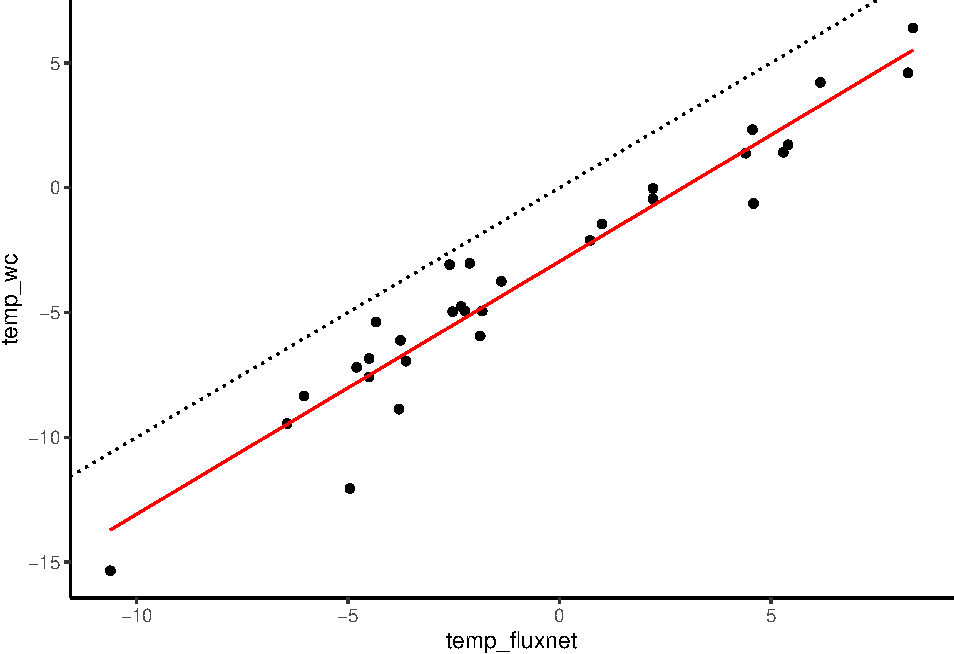
\includegraphics{esds_book_files/figure-latex/unnamed-chunk-58-1.pdf}

We compute the mean squared error.

\begin{Shaded}
\begin{Highlighting}[]
\KeywordTok{mse}\NormalTok{(df_sites_temp}\OperatorTok{$}\NormalTok{temp_fluxnet, df_sites_temp}\OperatorTok{$}\NormalTok{temp_wc)}
\end{Highlighting}
\end{Shaded}

\begin{verbatim}
## [1] 10.43716
\end{verbatim}

We see that Chelsa correlates better (because the mean squared error is smaller) with the temperature values at the towers. We also see that Worldclim compared to CHELSA tends to predict colder temperatures.

\textbf{Checkpoint}

Above, we compared the CHELSA temperatures with the tower temperatures. Now we want to visually see which of the two data had the higher mean for each tower location.
Plot the map of europe and add the tower locations as points. Colour the points so that for a higher CHESLA mean they are one colour and a higher tower temperature another.

\textbf{Solution}

\begin{Shaded}
\begin{Highlighting}[]
\CommentTok{# There are more way to do this but we used the function ifelse(). }
\CommentTok{# It takes 3 components: a condition, what to do if the condition applies and what to do if it doesn't apply.}

\CommentTok{# So here if chelsa temperatures are higher we want the point to be purple otherwise orange:}
\NormalTok{cols_chelsa_flux <-}\StringTok{ }\KeywordTok{ifelse}\NormalTok{(df_sites_temp}\OperatorTok{$}\NormalTok{temp_chelsa }\OperatorTok{>}\StringTok{ }\NormalTok{df_sites_temp}\OperatorTok{$}\NormalTok{temp_fluxnet,}\StringTok{"purple"}\NormalTok{,}\StringTok{"orange"}\NormalTok{)}

\CommentTok{# We could also do different shapes if we wanted...}
\NormalTok{pch_chelsa_flux <-}\StringTok{ }\KeywordTok{ifelse}\NormalTok{(df_sites_temp}\OperatorTok{$}\NormalTok{temp_chelsa }\OperatorTok{>}\StringTok{ }\NormalTok{df_sites_temp}\OperatorTok{$}\NormalTok{temp_fluxnet, }\DecValTok{19}\NormalTok{ ,}\DecValTok{17}\NormalTok{)}

\CommentTok{# Plot the result:}

\CommentTok{# plot(europe_shape)}
\CommentTok{# points(df_sites_temp$lon,df_sites_temp$lat, pch=pch_diff, col = col_checkpoint)}

\CommentTok{# OR with ggplot}

\KeywordTok{ggplot}\NormalTok{() }\OperatorTok{+}
\StringTok{  }\KeywordTok{geom_polygon}\NormalTok{(}\DataTypeTok{data =}\NormalTok{ europe_shape, }\KeywordTok{aes}\NormalTok{(}\DataTypeTok{x =}\NormalTok{ long, }\DataTypeTok{y =}\NormalTok{ lat, }\DataTypeTok{group =}\NormalTok{ group), }\DataTypeTok{fill=}\OtherTok{NA}\NormalTok{, }\DataTypeTok{colour =} \StringTok{"black"}\NormalTok{) }\OperatorTok{+}
\StringTok{  }\KeywordTok{geom_point}\NormalTok{(}\DataTypeTok{data =}\NormalTok{ df_sites_temp, }\KeywordTok{aes}\NormalTok{(}\DataTypeTok{x =}\NormalTok{ lon, }\DataTypeTok{y =}\NormalTok{ lat), }\DataTypeTok{color =}\NormalTok{ cols_chelsa_flux, }\DataTypeTok{shape =}\NormalTok{ pch_chelsa_flux, }\DataTypeTok{size=}\DecValTok{2}\NormalTok{) }\OperatorTok{+}
\StringTok{  }\KeywordTok{labs}\NormalTok{(}\DataTypeTok{x =} \StringTok{"Longitude"}\NormalTok{, }\DataTypeTok{y =} \StringTok{"Latitude"}\NormalTok{) }\OperatorTok{+}
\StringTok{  }\KeywordTok{theme_classic}\NormalTok{()}\OperatorTok{+}\StringTok{ }
\StringTok{  }\KeywordTok{coord_quickmap}\NormalTok{()}
\end{Highlighting}
\end{Shaded}

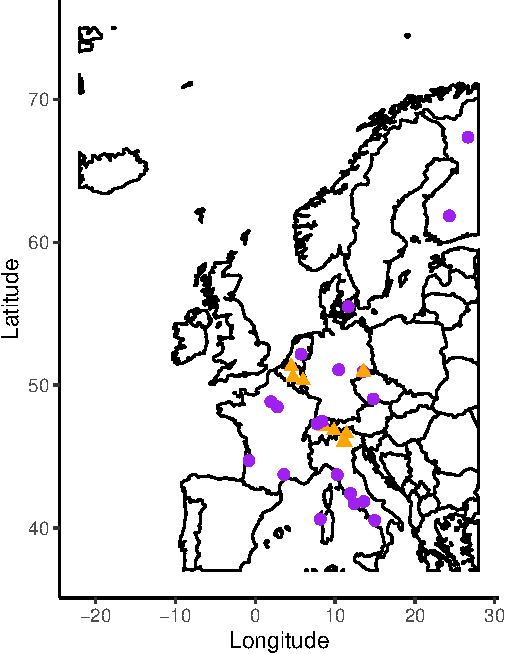
\includegraphics{esds_book_files/figure-latex/unnamed-chunk-60-1.pdf}

\hypertarget{correlations-with-gpp}{%
\subsubsection{Correlations with GPP}\label{correlations-with-gpp}}

We already had a look at GPP in Chapter 2. In this section we want to correlate Chelsa temperature and landcover with GPP.

In models we often take multiple variables and correlate them to another variable (here GPP). By seeing if they correlate well we can see if any of the variables make good so-called \emph{predictors}. Let's see how well landcover and temperature correlate with GPP.

We start off by extracting the mean GPP at the tower sites. To do this we group our data by the \emph{siteid} (or tower) and the year. This way we can get the GPP across a year and then an average across all years for each site.

\begin{Shaded}
\begin{Highlighting}[]
\NormalTok{GPP <-}\StringTok{ }\NormalTok{ddf_allsites_nested_joined }\OperatorTok\StringTok{ }
\StringTok{  }\KeywordTok{unnest}\NormalTok{(data) }\OperatorTok\StringTok{ }
\StringTok{  }\KeywordTok{mutate}\NormalTok{(}\DataTypeTok{year =} \KeywordTok{year}\NormalTok{(TIMESTAMP)) }\OperatorTok\StringTok{ }
\StringTok{  }\KeywordTok{group_by}\NormalTok{(siteid, year) }\OperatorTok\StringTok{ }
\StringTok{  }\KeywordTok{summarise}\NormalTok{(}\DataTypeTok{gpp_ann =} \KeywordTok{sum}\NormalTok{(GPP_NT_VUT_REF)) }\OperatorTok\StringTok{ }
\StringTok{  }\KeywordTok{ungroup}\NormalTok{() }\OperatorTok\StringTok{ }
\StringTok{  }\KeywordTok{group_by}\NormalTok{(siteid) }\OperatorTok\StringTok{ }
\StringTok{  }\KeywordTok{summarise}\NormalTok{(}\DataTypeTok{gpp_meanann =} \KeywordTok{mean}\NormalTok{(gpp_ann)) }\OperatorTok\StringTok{ }
\StringTok{  }\NormalTok{dplyr}\OperatorTok{::}\KeywordTok{select}\NormalTok{(siteid, gpp_meanann)}

\CommentTok{# we remove the data we don't have in the other datasets for the correlations}
\NormalTok{GPP <-}\StringTok{ }\NormalTok{GPP[}\OperatorTok{-}\KeywordTok{c}\NormalTok{(}\DecValTok{14}\NormalTok{, }\DecValTok{16}\NormalTok{, }\DecValTok{34}\NormalTok{), ]}
\end{Highlighting}
\end{Shaded}

We then extract landcover data at the tower sites.

\begin{Shaded}
\begin{Highlighting}[]
\NormalTok{df_sites_landcover <-}\StringTok{ }\KeywordTok{extract}\NormalTok{(raster_landcover, sp_sites, }\DataTypeTok{sp =} \OtherTok{TRUE}\NormalTok{)}
\NormalTok{df_sites_landcover <-}\StringTok{ }\KeywordTok{as.tibble}\NormalTok{(df_sites_landcover)}

\CommentTok{# we remove the sites we removed before}
\NormalTok{df_sites_landcover <-}\StringTok{ }\NormalTok{df_sites_landcover[}\OperatorTok{-}\KeywordTok{c}\NormalTok{(}\DecValTok{16}\NormalTok{, }\DecValTok{34}\NormalTok{), ]}
\end{Highlighting}
\end{Shaded}

And create a dataframe with all the extracted data from the tower sites to then make correlations.

\begin{Shaded}
\begin{Highlighting}[]
\NormalTok{landcover <-}\StringTok{ }\NormalTok{df_sites_landcover}\OperatorTok{$}\NormalTok{Globcover_EU}
\NormalTok{chelsa <-}\StringTok{ }\NormalTok{df_sites_temp}\OperatorTok{$}\NormalTok{temp_chelsa}
\NormalTok{df_corr <-}\StringTok{ }\KeywordTok{cbind}\NormalTok{(landcover, chelsa, GPP)}
\NormalTok{df_corr <-}\StringTok{ }\KeywordTok{as.data.frame}\NormalTok{(df_corr)}
\KeywordTok{head}\NormalTok{(df_corr)}
\end{Highlighting}
\end{Shaded}

\begin{verbatim}
##   landcover chelsa siteid gpp_meanann
## 1        50   1.85 BE-Bra          NA
## 2        20   0.95 BE-Lon    1348.667
## 3        90  -1.55 BE-Vie    1792.497
## 4       120  -0.15 CH-Cha    2478.429
## 5       140  -6.95 CH-Dav    1166.543
## 6        50  -3.25 CH-Fru    2106.319
\end{verbatim}

Though the landcover column contains numbers, it is actually categorical data. Each number represents a specific landcover type, so we add a column with the corresponding the landcover category name.

\begin{Shaded}
\begin{Highlighting}[]
\NormalTok{df_corr <-}\StringTok{ }\NormalTok{df_corr }\OperatorTok
\StringTok{  }\KeywordTok{mutate}\NormalTok{(}\DataTypeTok{landcover_cat =} \KeywordTok{case_when}\NormalTok{(landcover }\OperatorTok{==}\StringTok{ }\DecValTok{14} \OperatorTok{~}\StringTok{ "cropland"}\NormalTok{,}
\NormalTok{        landcover }\OperatorTok{==}\StringTok{ }\DecValTok{20} \OperatorTok{~}\StringTok{ "mosaic cropland"}\NormalTok{,}
\NormalTok{        landcover }\OperatorTok{==}\StringTok{ }\DecValTok{50} \OperatorTok{~}\StringTok{ "deciduous forest"}\NormalTok{,}
\NormalTok{        landcover }\OperatorTok{==}\StringTok{ }\DecValTok{70} \OperatorTok{~}\StringTok{ "evergreen forest"}\NormalTok{,}
\NormalTok{        landcover }\OperatorTok{==}\StringTok{ }\DecValTok{90} \OperatorTok{~}\StringTok{ "needleleaved forest"}\NormalTok{,}
\NormalTok{        landcover }\OperatorTok{==}\StringTok{ }\DecValTok{110} \OperatorTok{~}\StringTok{ "mosaic forest"}\NormalTok{,}
\NormalTok{        landcover }\OperatorTok{==}\StringTok{ }\DecValTok{120} \OperatorTok{~}\StringTok{ "mosaic forest/shrub/grass"}\NormalTok{,}
\NormalTok{        landcover }\OperatorTok{==}\StringTok{ }\DecValTok{130} \OperatorTok{~}\StringTok{ "mosaic shrubland"}\NormalTok{,}
\NormalTok{        landcover }\OperatorTok{==}\StringTok{ }\DecValTok{140} \OperatorTok{~}\StringTok{ "mosaic grassland"}\NormalTok{,}
\NormalTok{        landcover }\OperatorTok{==}\StringTok{ }\DecValTok{150} \OperatorTok{~}\StringTok{ "sparse vegetation"}\NormalTok{))}
\end{Highlighting}
\end{Shaded}

Back to correlations! Let's start by correlating the Chelsa temperatures with GPP. We do this by building a simple linear model using the function \texttt{lm()}.

\begin{Shaded}
\begin{Highlighting}[]
\NormalTok{reg1 <-}\StringTok{ }\KeywordTok{lm}\NormalTok{(gpp_meanann}\OperatorTok{~}\NormalTok{chelsa, }\DataTypeTok{data =}\NormalTok{ df_corr) }
\end{Highlighting}
\end{Shaded}

To visualise the correlation we plot our temperature data with the linear model.

\begin{Shaded}
\begin{Highlighting}[]
\NormalTok{df_corr }\OperatorTok\StringTok{ }
\StringTok{  }\KeywordTok{ggplot}\NormalTok{(}\KeywordTok{aes}\NormalTok{(}\DataTypeTok{x =}\NormalTok{ chelsa, }\DataTypeTok{y =}\NormalTok{ gpp_meanann)) }\OperatorTok{+}
\StringTok{  }\KeywordTok{geom_point}\NormalTok{() }\OperatorTok{+}
\StringTok{  }\KeywordTok{geom_smooth}\NormalTok{(}\DataTypeTok{method=}\StringTok{'lm'}\NormalTok{, }\DataTypeTok{color=}\StringTok{"red"}\NormalTok{, }\DataTypeTok{size=}\FloatTok{0.5}\NormalTok{, }\DataTypeTok{se=}\OtherTok{FALSE}\NormalTok{) }\OperatorTok{+}
\StringTok{  }\KeywordTok{xlab}\NormalTok{(}\StringTok{"Chelsa temperature"}\NormalTok{) }\OperatorTok{+}
\StringTok{  }\KeywordTok{ylab}\NormalTok{(}\StringTok{"GPP mean [µmolCO2 m-2 s-1]"}\NormalTok{) }\OperatorTok{+}
\StringTok{  }\KeywordTok{theme_classic}\NormalTok{()}
\end{Highlighting}
\end{Shaded}

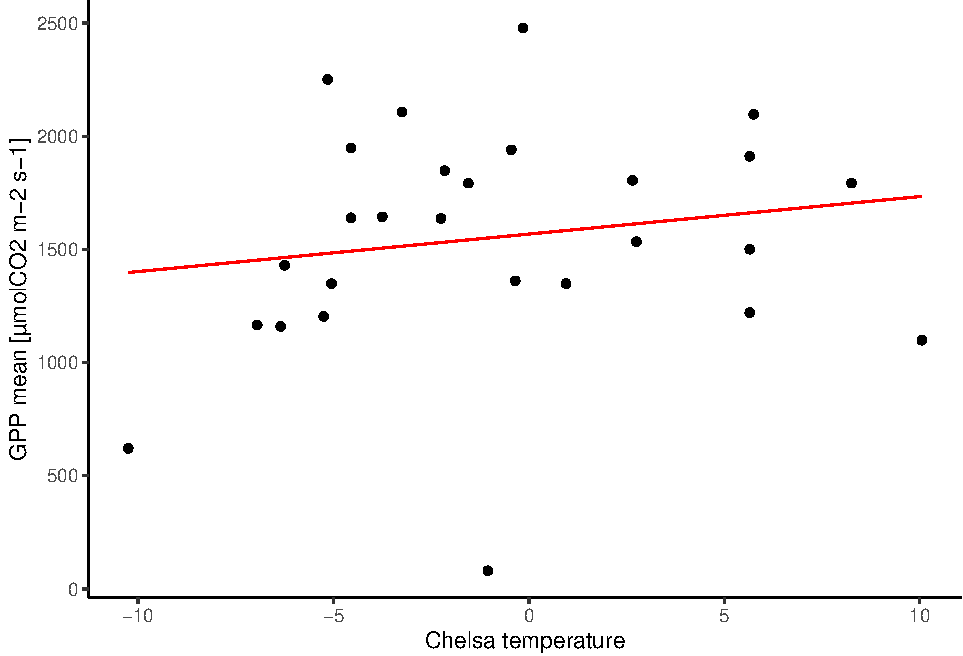
\includegraphics{esds_book_files/figure-latex/unnamed-chunk-66-1.pdf}

Then we make a linear model for GPP and landcover.

\begin{Shaded}
\begin{Highlighting}[]
\NormalTok{reg2 <-}\StringTok{ }\KeywordTok{lm}\NormalTok{(gpp_meanann}\OperatorTok{~}\NormalTok{landcover, }\DataTypeTok{data=}\NormalTok{df_corr)}
\end{Highlighting}
\end{Shaded}

\ldots{} and again plot it. However, since landcover is categorical data we make a boxplot instead. We've also added a general trendline but remember this could be quite different if we correclated data from a specific landcover category with GPP.

\begin{Shaded}
\begin{Highlighting}[]
\KeywordTok{ggplot}\NormalTok{(}\DataTypeTok{data=}\NormalTok{df_corr, }\KeywordTok{aes}\NormalTok{(}\DataTypeTok{x=}\NormalTok{landcover_cat, }\DataTypeTok{y=}\NormalTok{gpp_meanann, }\DataTypeTok{group=}\KeywordTok{as.factor}\NormalTok{(landcover_cat)))}\OperatorTok{+}\StringTok{ }
\StringTok{        }\KeywordTok{geom_boxplot}\NormalTok{() }\OperatorTok{+}\StringTok{ }
\StringTok{        }\KeywordTok{labs}\NormalTok{(}\DataTypeTok{x =} \StringTok{"Landcover Category"}\NormalTok{, }\DataTypeTok{y =} \StringTok{"GPP mean [µmolCO2 m-2 s-1]"}\NormalTok{) }\OperatorTok{+}
\StringTok{        }\KeywordTok{theme_classic}\NormalTok{() }\OperatorTok{+}
\StringTok{        }\KeywordTok{theme}\NormalTok{(}\DataTypeTok{axis.text.x =} \KeywordTok{element_text}\NormalTok{(}\DataTypeTok{angle =} \DecValTok{90}\NormalTok{, }\DataTypeTok{size=}\DecValTok{12}\NormalTok{))}
\end{Highlighting}
\end{Shaded}

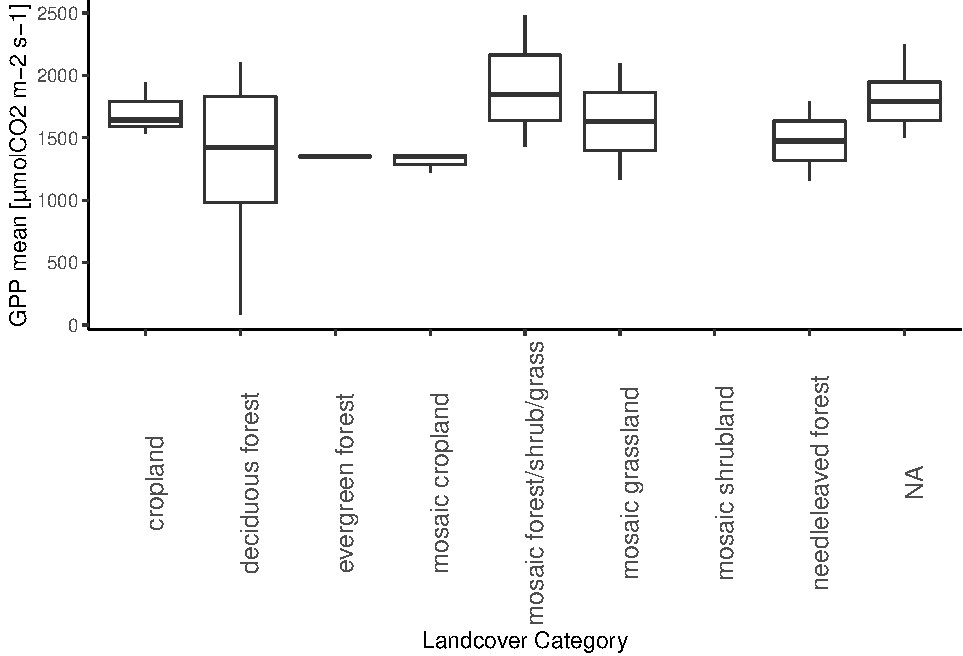
\includegraphics{esds_book_files/figure-latex/unnamed-chunk-68-1.pdf}

We don't see a particularly strong correlation, thus we need to consider other predictors and more complex models. You will discuss that later in the class.

\hypertarget{key-points-of-the-tutorial}{%
\subsection{Key points of the tutorial}\label{key-points-of-the-tutorial}}

Integrating remote sensing data: we extract NDVI in the area around our eddy flux towers from the MODISTools package and conver it into a raster format.

\begin{itemize}
\tightlist
\item
  Collapse NDVI measured within an area around the eddy flux towers to calculate the mean across years
\item
  Merge this temporal data with our eddy flux data
\item
  Apply linear regression to test whether the addition of NDVI data to our model of GPP and PPFD\_IN improves its accuracy
\end{itemize}

Points:
the eddy flux tower sites are plotted as points on a map of Europe.

\begin{itemize}
\tightlist
\item
  Extract coordinates of the tower sites from the metadata
\item
  Transform the points into SpatialPoints with the sp package and plot them on a map of Europe
\end{itemize}

Shapefiles: we add country and border information to our tower site plots.

\begin{itemize}
\tightlist
\item
  Extract the information about the spatial polygons in the europe\_shape shapefile and apply one coordinate reference system
\item
  Add the SpatialPoints matrix and shapefile data europe\_shape to the tower site dataframe
\item
  Filter out the countries with towers and visualize only them
\end{itemize}

Rasters: we investigate whether the variables landcover and temperature can explain GPP.

\begin{itemize}
\tightlist
\item
  Load landcover data from Globcover temperature data from CHELSA in the form of rasters and plot them around our tower sites with the raster and rasterVis packages
\item
  Apply the same resolution (aggregate) and origin (align) to the climate and landcover rasters
\item
  Compare modeled climate data from CHELSA and Worldclim to our fluxnet data by extracting the temperatures at the tower sites and calculating the MSE
\item
  Finally, landcover and CHELSA modeled temperatures are plugged into a linear regression to see if they are significantly correlated with GPP
\end{itemize}

Bonus: here we incorporate plant species data from GBIF to determine their effect on GPP with the help of PCA.

\begin{itemize}
\tightlist
\item
  Create a presence-absence matrix for all locations and species
\item
  Check species data for possible sampling biases by visualizing the number of occurrence records
\item
  Plot species richness on the map
\item
  Add species traits to our dataset with a for loop
\item
  Use PCA to determine which traits explain the most variation in GPP
\end{itemize}

\hypertarget{bonus-species-occurrence-trait-data-and-pcas}{%
\subsection{Bonus: Species Occurrence, Trait Data and PCAs}\label{bonus-species-occurrence-trait-data-and-pcas}}

In functional ecology, we focus on the function that a species has in a community. This sub-discipline of ecology represents the intersection between ecological patterns and the mechanisms that underlie them and focuses on traits represented in large number of species. Here, we use plant distribution data around the fluxnet towers to investigate the plant community composition for each location. The community composition will allow us to get insights on which plant traits that are dominant. This is relevant because plant traits are both responsive to local climate and strong predictors of primary productivity. For example, Specific Leaf Area (SLA) and plant height, are linked to GPP and affected by local climate. Functional traits capture core differences in the strategies plants use to acquire and invest resources. Most woody plants have the same basic physiological function and key resource requirements, however species differ considerably in the rates at which resources are acquired, invested into different tissues, and lost via turnover. Traits for example moderate plant responses to light environment and determine shade tolerance. They have been shown to affect growth depending on plant size. In the first step, we use distribution data from the Global Biodiversity Information Facility (GBIF) to obtain the community composition in each location.

GBIF is an international organization that makes biodiversity data publicly available. The data are provided by many institutions from around the world and GBIF gathers these data and makes them accessible and searchable through their platform. Data available on GBIF are primarily distribution records on plants, animals, fungi, and microbes for the world, and scientific names data. This is very useful information for ecological analysis. With the ``rgbif'' package we can download occurrence data directly from the GBIF database to R.

\hypertarget{species-occurrences}{%
\paragraph{Species Occurrences}\label{species-occurrences}}

We start by to loading the relevant packages.

\begin{Shaded}
\begin{Highlighting}[]
\KeywordTok{library}\NormalTok{(rgbif)}
\KeywordTok{library}\NormalTok{(rgeos)}
\end{Highlighting}
\end{Shaded}

In this first, section we will give you an example of how to download data from gbif for the CH-Lae site.

\begin{Shaded}
\begin{Highlighting}[]
\CommentTok{# combine the CH-Lae latitude and longitude}
\NormalTok{CHLae_lonlat <-}\StringTok{ }\KeywordTok{as.data.frame}\NormalTok{(}\KeywordTok{cbind}\NormalTok{(}\DataTypeTok{longitude=}\NormalTok{lon_lae, }\DataTypeTok{latitude=}\NormalTok{lat_lae))}

\CommentTok{# make them into 'SpatialPoints', this is an alternative method to the one used above}
\KeywordTok{coordinates}\NormalTok{(CHLae_lonlat) <-}\StringTok{ }\ErrorTok{~}\NormalTok{longitude }\OperatorTok{+}\StringTok{ }\NormalTok{latitude}

\CommentTok{# assign a projection and coordinate reference system}
\KeywordTok{crs}\NormalTok{(CHLae_lonlat) <-}\StringTok{ "+init=epsg:4326 +proj=longlat +datum=WGS84 +no_defs"}

\CommentTok{# create a roughly 5.5km buffer around the CH-Lae tower}
\NormalTok{TowerBuffer <-}\StringTok{ }\KeywordTok{gBuffer}\NormalTok{(CHLae_lonlat, }\DataTypeTok{width=}\FloatTok{0.05}\NormalTok{)}

\CommentTok{# transform the tower buffer into polygons}
\NormalTok{tower.polygon <-}\StringTok{ }\KeywordTok{polygons}\NormalTok{(TowerBuffer)}
\end{Highlighting}
\end{Shaded}

Then transform the polygon to wkt format which is needed for the gbif input:

\begin{Shaded}
\begin{Highlighting}[]
\NormalTok{tower.polygon.wkt <-}\StringTok{ }\KeywordTok{writeWKT}\NormalTok{(tower.polygon)}
\end{Highlighting}
\end{Shaded}

Now we are ready to download occurrence records of plants around the CH-Lae tower from gbif with \texttt{occ\_search()} function.
We add the hasCoordinate = T, to make sure we only download data with coordinates.
The \emph{geometry} argument will be equal to our constructed polygon of the buffer.

\begin{Shaded}
\begin{Highlighting}[]
\NormalTok{occ_CHlae <-}\StringTok{ }\KeywordTok{occ_data}\NormalTok{(}\DataTypeTok{taxonKey =} \DecValTok{7707728}\NormalTok{, }\DataTypeTok{hasCoordinate =}\NormalTok{ T, }
                     \DataTypeTok{geometry =}\NormalTok{ tower.polygon.wkt, }\DataTypeTok{limit =} \DecValTok{50000}\NormalTok{)}

\CommentTok{# The output is a list so we extract the actual data since this is of interest}
\NormalTok{occ_CHlae <-}\StringTok{ }\KeywordTok{as.data.frame}\NormalTok{(occ_CHlae}\OperatorTok{$}\NormalTok{data)}
\end{Highlighting}
\end{Shaded}

\begin{verbatim}
##          key                 scientificName decimalLatitude decimalLongitude
## 1 3028451251 Berberis julianae C.K.Schneid.        47.46482         8.333900
## 2 2646869619            Corylus avellana L.        47.44893         8.356892
## 3 2649395661             Daphne laureola L.        47.48192         8.317558
## 4 2649628860                Hedera helix L.        47.50389         8.346389
## 5 2878758835       Asplenium trichomanes L.        47.46482         8.333900
## 6 2878758840            Thlaspi montanum L.        47.46482         8.333900
##         issues                           datasetKey
## 1              83fdfd3d-3a25-4705-9fbe-3db1d1892b13
## 2 cdround,cudc 14d5676a-2c54-4f94-9023-1e8dcd822aa0
## 3 cdround,cudc 14d5676a-2c54-4f94-9023-1e8dcd822aa0
## 4 cdround,cudc 14d5676a-2c54-4f94-9023-1e8dcd822aa0
## 5              83fdfd3d-3a25-4705-9fbe-3db1d1892b13
## 6              83fdfd3d-3a25-4705-9fbe-3db1d1892b13
##                       publishingOrgKey                      installationKey
## 1 64ee55c9-570a-42af-b7da-3f13c6b4e5a9 dc9d8bd0-3c20-4fba-b7ff-26d654817ea7
## 2 da86174a-a605-43a4-a5e8-53d484152cd3 fe1a98a6-82b8-4652-86d6-d0f938207f67
## 3 da86174a-a605-43a4-a5e8-53d484152cd3 fe1a98a6-82b8-4652-86d6-d0f938207f67
## 4 da86174a-a605-43a4-a5e8-53d484152cd3 fe1a98a6-82b8-4652-86d6-d0f938207f67
## 5 64ee55c9-570a-42af-b7da-3f13c6b4e5a9 dc9d8bd0-3c20-4fba-b7ff-26d654817ea7
## 6 64ee55c9-570a-42af-b7da-3f13c6b4e5a9 dc9d8bd0-3c20-4fba-b7ff-26d654817ea7
##   publishingCountry    protocol                   lastCrawled
## 1                CH DWC_ARCHIVE 2021-02-02T15:59:13.567+00:00
## 2                FR DWC_ARCHIVE 2020-12-10T14:09:16.521+00:00
## 3                FR DWC_ARCHIVE 2020-12-10T14:09:16.521+00:00
## 4                FR DWC_ARCHIVE 2020-12-10T14:09:16.521+00:00
## 5                CH DWC_ARCHIVE 2021-02-02T15:59:13.567+00:00
## 6                CH DWC_ARCHIVE 2021-02-02T15:59:13.567+00:00
##                      lastParsed crawlId               hostingOrganizationKey
## 1 2021-02-02T16:35:54.759+00:00      17 23e067c0-a255-11da-beae-b8a03c50a862
## 2 2020-12-15T17:21:35.615+00:00      22 da86174a-a605-43a4-a5e8-53d484152cd3
## 3 2020-12-15T17:22:27.362+00:00      22 da86174a-a605-43a4-a5e8-53d484152cd3
## 4 2020-12-15T17:22:28.963+00:00      22 da86174a-a605-43a4-a5e8-53d484152cd3
## 5 2021-02-02T16:36:21.675+00:00      17 23e067c0-a255-11da-beae-b8a03c50a862
## 6 2021-02-02T16:35:36.344+00:00      17 23e067c0-a255-11da-beae-b8a03c50a862
##   extensions     basisOfRecord occurrenceStatus taxonKey kingdomKey phylumKey
## 1       none HUMAN_OBSERVATION          PRESENT  3981543          6   7707728
## 2       none HUMAN_OBSERVATION          PRESENT  2875979          6   7707728
## 3       none HUMAN_OBSERVATION          PRESENT  5420853          6   7707728
## 4       none HUMAN_OBSERVATION          PRESENT  8351737          6   7707728
## 5       none HUMAN_OBSERVATION          PRESENT  8108066          6   7707728
## 6       none HUMAN_OBSERVATION          PRESENT  3045290          6   7707728
##   classKey orderKey familyKey genusKey speciesKey acceptedTaxonKey
## 1      220      399      6673  3033893    3981543          3981543
## 2      220     1354      4688  2875967    2875979          2875979
## 3      220      941      2428  3188453    5420853          5420853
## 4      220     1351      8800  3036021    8351737          8351737
## 5  7228684      392      6625  2650583    8108066          8108066
## 6      220  7225535      3112  3045219    3045261          3045261
##            acceptedScientificName kingdom       phylum        order
## 1  Berberis julianae C.K.Schneid. Plantae Tracheophyta Ranunculales
## 2             Corylus avellana L. Plantae Tracheophyta      Fagales
## 3              Daphne laureola L. Plantae Tracheophyta     Malvales
## 4                 Hedera helix L. Plantae Tracheophyta      Apiales
## 5        Asplenium trichomanes L. Plantae Tracheophyta Polypodiales
## 6 Noccaea fendleri (A.Gray) Holub Plantae Tracheophyta  Brassicales
##          family     genus               species genericName specificEpithet
## 1 Berberidaceae  Berberis     Berberis julianae    Berberis        julianae
## 2    Betulaceae   Corylus      Corylus avellana     Corylus        avellana
## 3 Thymelaeaceae    Daphne       Daphne laureola      Daphne        laureola
## 4    Araliaceae    Hedera          Hedera helix      Hedera           helix
## 5  Aspleniaceae Asplenium Asplenium trichomanes   Asplenium     trichomanes
## 6  Brassicaceae   Noccaea      Noccaea fendleri     Thlaspi        montanum
##   taxonRank taxonomicStatus coordinateUncertaintyInMeters elevation
## 1   SPECIES        ACCEPTED                          3535     366.5
## 2   SPECIES        ACCEPTED                            23        NA
## 3   SPECIES        ACCEPTED                            65        NA
## 4   SPECIES        ACCEPTED                            NA        NA
## 5   SPECIES        ACCEPTED                          3535     610.0
## 6   SPECIES         SYNONYM                          3535     550.0
##   elevationAccuracy stateProvince year month           eventDate
## 1               1.5            Ag 2021     1 2021-01-01T00:00:00
## 2                NA          <NA> 2020     1 2020-01-18T12:23:07
## 3                NA          <NA> 2020     1 2020-01-06T09:52:11
## 4                NA          <NA> 2020     1 2020-01-18T17:48:09
## 5                NA            Ag 2020     1 2020-01-02T00:00:00
## 6                NA            Ag 2020     1 2020-01-02T00:00:00
##                 lastInterpreted
## 1 2021-02-02T16:35:54.759+00:00
## 2 2020-12-15T17:21:35.615+00:00
## 3 2020-12-15T17:22:27.362+00:00
## 4 2020-12-15T17:22:28.963+00:00
## 5 2021-02-02T16:36:21.675+00:00
## 6 2021-02-02T16:35:36.344+00:00
##                                                license identifiers facts
## 1 http://creativecommons.org/licenses/by/4.0/legalcode        none  none
## 2 http://creativecommons.org/licenses/by/4.0/legalcode        none  none
## 3 http://creativecommons.org/licenses/by/4.0/legalcode        none  none
## 4 http://creativecommons.org/licenses/by/4.0/legalcode        none  none
## 5 http://creativecommons.org/licenses/by/4.0/legalcode        none  none
## 6 http://creativecommons.org/licenses/by/4.0/legalcode        none  none
##   relations gadm.level0.gid gadm.level0.name gadm.level1.gid gadm.level1.name
## 1      none             CHE      Switzerland         CHE.1_1           Aargau
## 2      none             CHE      Switzerland         CHE.1_1           Aargau
## 3      none             CHE      Switzerland         CHE.1_1           Aargau
## 4      none             CHE      Switzerland         CHE.1_1           Aargau
## 5      none             CHE      Switzerland         CHE.1_1           Aargau
## 6      none             CHE      Switzerland         CHE.1_1           Aargau
##   gadm.level2.gid gadm.level2.name gadm.level3.gid gadm.level3.name isInCluster
## 1       CHE.1.2_1            Baden    CHE.1.2.23_1        Wettingen       FALSE
## 2       CHE.1.2_1            Baden    CHE.1.2.26_1         Würenlos       FALSE
## 3       CHE.1.2_1            Baden     CHE.1.2.6_1       Ennetbaden       FALSE
## 4       CHE.1.2_1            Baden     CHE.1.2.5_1      Ehrendingen       FALSE
## 5       CHE.1.2_1            Baden    CHE.1.2.23_1        Wettingen       FALSE
## 6       CHE.1.2_1            Baden    CHE.1.2.23_1        Wettingen       FALSE
##   geodeticDatum          class countryCode recordedByIDs identifiedByIDs
## 1         WGS84  Magnoliopsida          CH          none            none
## 2         WGS84  Magnoliopsida          CH          none            none
## 3         WGS84  Magnoliopsida          CH          none            none
## 4         WGS84  Magnoliopsida          CH          none            none
## 5         WGS84 Polypodiopsida          CH          none            none
## 6         WGS84  Magnoliopsida          CH          none            none
##       country rightsHolder              identifier nomenclaturalCode
## 1 Switzerland   Info Flora INFOFLORA-TRAC-10029158               ICN
## 2 Switzerland         <NA>           q-10128206654              <NA>
## 3 Switzerland         <NA>           q-10127072482              <NA>
## 4 Switzerland         <NA>           q-10128246487              <NA>
## 5 Switzerland   Info Flora  INFOFLORA-TRAC-8884922               ICN
## 6 Switzerland   Info Flora  INFOFLORA-TRAC-8885363               ICN
##      georeferencedBy
## 1 observer/collector
## 2               <NA>
## 3               <NA>
## 4               <NA>
## 5 observer/collector
## 6 observer/collector
##                                                                                                                                                                                                                                                                        dataGeneralizations
## 1 In order to respect the currently nationally agreed ethical framework while simultaneously sharing scientifically utilizable data for large scale studies, Swiss biodiversity data is generally published generalized to 5km grid squares. Altitude information corresponds to raw data.
## 2                                                                                                                                                                                                                                                                                     <NA>
## 3                                                                                                                                                                                                                                                                                     <NA>
## 4                                                                                                                                                                                                                                                                                     <NA>
## 5 In order to respect the currently nationally agreed ethical framework while simultaneously sharing scientifically utilizable data for large scale studies, Swiss biodiversity data is generally published generalized to 5km grid squares. Altitude information corresponds to raw data.
## 6 In order to respect the currently nationally agreed ethical framework while simultaneously sharing scientifically utilizable data for large scale studies, Swiss biodiversity data is generally published generalized to 5km grid squares. Altitude information corresponds to raw data.
##                                  datasetName     gbifID            occurrenceID
## 1 Swiss National Databank of Vascular Plants 3028451251 INFOFLORA-TRAC-10029158
## 2                                       <NA> 2646869619           q-10128206654
## 3                                       <NA> 2649395661           q-10127072482
## 4                                       <NA> 2649628860           q-10128246487
## 5 Swiss National Databank of Vascular Plants 2878758835  INFOFLORA-TRAC-8884922
## 6 Swiss National Databank of Vascular Plants 2878758840  INFOFLORA-TRAC-8885363
##                           taxonID           catalogNumber       recordedBy
## 1  infospecies.ch:infoflora:59155 INFOFLORA-TRAC-10029158        anonymous
## 2                            <NA>                    <NA>             <NA>
## 3                            <NA>                    <NA>             <NA>
## 4                            <NA>                    <NA>             <NA>
## 5  infospecies.ch:infoflora:51400  INFOFLORA-TRAC-8884922 Werner Christian
## 6 infospecies.ch:infoflora:418700  INFOFLORA-TRAC-8885363 Werner Christian
##   institutionCode      datasetID
## 1       INFOFLORA INFOFLORA-TRAC
## 2            <NA>           <NA>
## 3            <NA>           <NA>
## 4            <NA>           <NA>
## 5       INFOFLORA INFOFLORA-TRAC
## 6       INFOFLORA INFOFLORA-TRAC
##                                                                   bibliographicCitation
## 1      Info Flora (2021-02-01) INFOFLORA-TRAC-10029158. Plantes vasculaires, Info Flora
## 2                                                                                  <NA>
## 3                                                                                  <NA>
## 4                                                                                  <NA>
## 5 Christian Werner (2021-02-01) INFOFLORA-TRAC-8884922. Plantes vasculaires, Info Flora
## 6 Christian Werner (2021-02-01) INFOFLORA-TRAC-8885363. Plantes vasculaires, Info Flora
##                             name projectId individualCount day fieldNumber
## 1 Berberis julianae C.K.Schneid.      <NA>              NA  NA        <NA>
## 2            Corylus avellana L.   queries               1  18        <NA>
## 3             Daphne laureola L.   queries               1   6        <NA>
## 4                Hedera helix L.   queries               1  18        <NA>
## 5       Asplenium trichomanes L.      <NA>              NA   2        <NA>
## 6            Thlaspi montanum L.      <NA>              NA   2        <NA>
##   extensions.http...rs.gbif.org.terms.1.0.Multimedia.http...purl.org.dc.terms.rightsHolder
## 1                                                                                     <NA>
## 2                                                                                     <NA>
## 3                                                                                     <NA>
## 4                                                                                     <NA>
## 5                                                                                     <NA>
## 6                                                                                     <NA>
##   extensions.http...rs.gbif.org.terms.1.0.Multimedia.http...purl.org.dc.terms.identifier
## 1                                                                                   <NA>
## 2                                                                                   <NA>
## 3                                                                                   <NA>
## 4                                                                                   <NA>
## 5                                                                                   <NA>
## 6                                                                                   <NA>
##   extensions.http...rs.gbif.org.terms.1.0.Multimedia.http...purl.org.dc.terms.type
## 1                                                                             <NA>
## 2                                                                             <NA>
## 3                                                                             <NA>
## 4                                                                             <NA>
## 5                                                                             <NA>
## 6                                                                             <NA>
##   extensions.http...rs.gbif.org.terms.1.0.Multimedia.http...rs.tdwg.org.dwc.terms.catalogNumber
## 1                                                                                          <NA>
## 2                                                                                          <NA>
## 3                                                                                          <NA>
## 4                                                                                          <NA>
## 5                                                                                          <NA>
## 6                                                                                          <NA>
##   extensions.http...rs.gbif.org.terms.1.0.Multimedia.http...purl.org.dc.terms.publisher
## 1                                                                                  <NA>
## 2                                                                                  <NA>
## 3                                                                                  <NA>
## 4                                                                                  <NA>
## 5                                                                                  <NA>
## 6                                                                                  <NA>
##   extensions.http...rs.gbif.org.terms.1.0.Multimedia.http...purl.org.dc.terms.license
## 1                                                                                <NA>
## 2                                                                                <NA>
## 3                                                                                <NA>
## 4                                                                                <NA>
## 5                                                                                <NA>
## 6                                                                                <NA>
##   extensions.http...rs.gbif.org.terms.1.0.Multimedia.http...purl.org.dc.terms.created
## 1                                                                                <NA>
## 2                                                                                <NA>
## 3                                                                                <NA>
## 4                                                                                <NA>
## 5                                                                                <NA>
## 6                                                                                <NA>
##   extensions.http...rs.gbif.org.terms.1.0.Multimedia.http...purl.org.dc.terms.format
## 1                                                                               <NA>
## 2                                                                               <NA>
## 3                                                                               <NA>
## 4                                                                               <NA>
## 5                                                                               <NA>
## 6                                                                               <NA>
##   extensions.http...rs.gbif.org.terms.1.0.Multimedia.http...purl.org.dc.terms.references
## 1                                                                                   <NA>
## 2                                                                                   <NA>
## 3                                                                                   <NA>
## 4                                                                                   <NA>
## 5                                                                                   <NA>
## 6                                                                                   <NA>
##   extensions.http...rs.gbif.org.terms.1.0.Multimedia.http...purl.org.dc.terms.creator
## 1                                                                                <NA>
## 2                                                                                <NA>
## 3                                                                                <NA>
## 4                                                                                <NA>
## 5                                                                                <NA>
## 6                                                                                <NA>
##   extensions.http...rs.gbif.org.terms.1.0.Multimedia.http...purl.org.dc.terms.rightsHolder.1
## 1                                                                                       <NA>
## 2                                                                                       <NA>
## 3                                                                                       <NA>
## 4                                                                                       <NA>
## 5                                                                                       <NA>
## 6                                                                                       <NA>
##   extensions.http...rs.gbif.org.terms.1.0.Multimedia.http...purl.org.dc.terms.identifier.1
## 1                                                                                     <NA>
## 2                                                                                     <NA>
## 3                                                                                     <NA>
## 4                                                                                     <NA>
## 5                                                                                     <NA>
## 6                                                                                     <NA>
##   extensions.http...rs.gbif.org.terms.1.0.Multimedia.http...purl.org.dc.terms.type.1
## 1                                                                               <NA>
## 2                                                                               <NA>
## 3                                                                               <NA>
## 4                                                                               <NA>
## 5                                                                               <NA>
## 6                                                                               <NA>
##   extensions.http...rs.gbif.org.terms.1.0.Multimedia.http...rs.tdwg.org.dwc.terms.catalogNumber.1
## 1                                                                                            <NA>
## 2                                                                                            <NA>
## 3                                                                                            <NA>
## 4                                                                                            <NA>
## 5                                                                                            <NA>
## 6                                                                                            <NA>
##   extensions.http...rs.gbif.org.terms.1.0.Multimedia.http...purl.org.dc.terms.publisher.1
## 1                                                                                    <NA>
## 2                                                                                    <NA>
## 3                                                                                    <NA>
## 4                                                                                    <NA>
## 5                                                                                    <NA>
## 6                                                                                    <NA>
##   extensions.http...rs.gbif.org.terms.1.0.Multimedia.http...purl.org.dc.terms.license.1
## 1                                                                                  <NA>
## 2                                                                                  <NA>
## 3                                                                                  <NA>
## 4                                                                                  <NA>
## 5                                                                                  <NA>
## 6                                                                                  <NA>
##   extensions.http...rs.gbif.org.terms.1.0.Multimedia.http...purl.org.dc.terms.created.1
## 1                                                                                  <NA>
## 2                                                                                  <NA>
## 3                                                                                  <NA>
## 4                                                                                  <NA>
## 5                                                                                  <NA>
## 6                                                                                  <NA>
##   extensions.http...rs.gbif.org.terms.1.0.Multimedia.http...purl.org.dc.terms.format.1
## 1                                                                                 <NA>
## 2                                                                                 <NA>
## 3                                                                                 <NA>
## 4                                                                                 <NA>
## 5                                                                                 <NA>
## 6                                                                                 <NA>
##   extensions.http...rs.gbif.org.terms.1.0.Multimedia.http...purl.org.dc.terms.references.1
## 1                                                                                     <NA>
## 2                                                                                     <NA>
## 3                                                                                     <NA>
## 4                                                                                     <NA>
## 5                                                                                     <NA>
## 6                                                                                     <NA>
##   extensions.http...rs.gbif.org.terms.1.0.Multimedia.http...purl.org.dc.terms.creator.1
## 1                                                                                  <NA>
## 2                                                                                  <NA>
## 3                                                                                  <NA>
## 4                                                                                  <NA>
## 5                                                                                  <NA>
## 6                                                                                  <NA>
##   extensions.http...rs.gbif.org.terms.1.0.Multimedia.http...purl.org.dc.terms.rightsHolder.2
## 1                                                                                       <NA>
## 2                                                                                       <NA>
## 3                                                                                       <NA>
## 4                                                                                       <NA>
## 5                                                                                       <NA>
## 6                                                                                       <NA>
##   extensions.http...rs.gbif.org.terms.1.0.Multimedia.http...purl.org.dc.terms.identifier.2
## 1                                                                                     <NA>
## 2                                                                                     <NA>
## 3                                                                                     <NA>
## 4                                                                                     <NA>
## 5                                                                                     <NA>
## 6                                                                                     <NA>
##   extensions.http...rs.gbif.org.terms.1.0.Multimedia.http...purl.org.dc.terms.type.2
## 1                                                                               <NA>
## 2                                                                               <NA>
## 3                                                                               <NA>
## 4                                                                               <NA>
## 5                                                                               <NA>
## 6                                                                               <NA>
##   extensions.http...rs.gbif.org.terms.1.0.Multimedia.http...rs.tdwg.org.dwc.terms.catalogNumber.2
## 1                                                                                            <NA>
## 2                                                                                            <NA>
## 3                                                                                            <NA>
## 4                                                                                            <NA>
## 5                                                                                            <NA>
## 6                                                                                            <NA>
##   extensions.http...rs.gbif.org.terms.1.0.Multimedia.http...purl.org.dc.terms.publisher.2
## 1                                                                                    <NA>
## 2                                                                                    <NA>
## 3                                                                                    <NA>
## 4                                                                                    <NA>
## 5                                                                                    <NA>
## 6                                                                                    <NA>
##   extensions.http...rs.gbif.org.terms.1.0.Multimedia.http...purl.org.dc.terms.license.2
## 1                                                                                  <NA>
## 2                                                                                  <NA>
## 3                                                                                  <NA>
## 4                                                                                  <NA>
## 5                                                                                  <NA>
## 6                                                                                  <NA>
##   extensions.http...rs.gbif.org.terms.1.0.Multimedia.http...purl.org.dc.terms.created.2
## 1                                                                                  <NA>
## 2                                                                                  <NA>
## 3                                                                                  <NA>
## 4                                                                                  <NA>
## 5                                                                                  <NA>
## 6                                                                                  <NA>
##   extensions.http...rs.gbif.org.terms.1.0.Multimedia.http...purl.org.dc.terms.format.2
## 1                                                                                 <NA>
## 2                                                                                 <NA>
## 3                                                                                 <NA>
## 4                                                                                 <NA>
## 5                                                                                 <NA>
## 6                                                                                 <NA>
##   extensions.http...rs.gbif.org.terms.1.0.Multimedia.http...purl.org.dc.terms.references.2
## 1                                                                                     <NA>
## 2                                                                                     <NA>
## 3                                                                                     <NA>
## 4                                                                                     <NA>
## 5                                                                                     <NA>
## 6                                                                                     <NA>
##   extensions.http...rs.gbif.org.terms.1.0.Multimedia.http...purl.org.dc.terms.creator.2
## 1                                                                                  <NA>
## 2                                                                                  <NA>
## 3                                                                                  <NA>
## 4                                                                                  <NA>
## 5                                                                                  <NA>
## 6                                                                                  <NA>
##   extensions.http...rs.gbif.org.terms.1.0.Multimedia.http...purl.org.dc.terms.rightsHolder.3
## 1                                                                                       <NA>
## 2                                                                                       <NA>
## 3                                                                                       <NA>
## 4                                                                                       <NA>
## 5                                                                                       <NA>
## 6                                                                                       <NA>
##   extensions.http...rs.gbif.org.terms.1.0.Multimedia.http...purl.org.dc.terms.identifier.3
## 1                                                                                     <NA>
## 2                                                                                     <NA>
## 3                                                                                     <NA>
## 4                                                                                     <NA>
## 5                                                                                     <NA>
## 6                                                                                     <NA>
##   extensions.http...rs.gbif.org.terms.1.0.Multimedia.http...purl.org.dc.terms.type.3
## 1                                                                               <NA>
## 2                                                                               <NA>
## 3                                                                               <NA>
## 4                                                                               <NA>
## 5                                                                               <NA>
## 6                                                                               <NA>
##   extensions.http...rs.gbif.org.terms.1.0.Multimedia.http...rs.tdwg.org.dwc.terms.catalogNumber.3
## 1                                                                                            <NA>
## 2                                                                                            <NA>
## 3                                                                                            <NA>
## 4                                                                                            <NA>
## 5                                                                                            <NA>
## 6                                                                                            <NA>
##   extensions.http...rs.gbif.org.terms.1.0.Multimedia.http...purl.org.dc.terms.publisher.3
## 1                                                                                    <NA>
## 2                                                                                    <NA>
## 3                                                                                    <NA>
## 4                                                                                    <NA>
## 5                                                                                    <NA>
## 6                                                                                    <NA>
##   extensions.http...rs.gbif.org.terms.1.0.Multimedia.http...purl.org.dc.terms.license.3
## 1                                                                                  <NA>
## 2                                                                                  <NA>
## 3                                                                                  <NA>
## 4                                                                                  <NA>
## 5                                                                                  <NA>
## 6                                                                                  <NA>
##   extensions.http...rs.gbif.org.terms.1.0.Multimedia.http...purl.org.dc.terms.created.3
## 1                                                                                  <NA>
## 2                                                                                  <NA>
## 3                                                                                  <NA>
## 4                                                                                  <NA>
## 5                                                                                  <NA>
## 6                                                                                  <NA>
##   extensions.http...rs.gbif.org.terms.1.0.Multimedia.http...purl.org.dc.terms.format.3
## 1                                                                                 <NA>
## 2                                                                                 <NA>
## 3                                                                                 <NA>
## 4                                                                                 <NA>
## 5                                                                                 <NA>
## 6                                                                                 <NA>
##   extensions.http...rs.gbif.org.terms.1.0.Multimedia.http...purl.org.dc.terms.references.3
## 1                                                                                     <NA>
## 2                                                                                     <NA>
## 3                                                                                     <NA>
## 4                                                                                     <NA>
## 5                                                                                     <NA>
## 6                                                                                     <NA>
##   extensions.http...rs.gbif.org.terms.1.0.Multimedia.http...purl.org.dc.terms.creator.3
## 1                                                                                  <NA>
## 2                                                                                  <NA>
## 3                                                                                  <NA>
## 4                                                                                  <NA>
## 5                                                                                  <NA>
## 6                                                                                  <NA>
##   extensions.http...rs.gbif.org.terms.1.0.Multimedia.http...purl.org.dc.terms.rightsHolder.4
## 1                                                                                       <NA>
## 2                                                                                       <NA>
## 3                                                                                       <NA>
## 4                                                                                       <NA>
## 5                                                                                       <NA>
## 6                                                                                       <NA>
##   extensions.http...rs.gbif.org.terms.1.0.Multimedia.http...purl.org.dc.terms.identifier.4
## 1                                                                                     <NA>
## 2                                                                                     <NA>
## 3                                                                                     <NA>
## 4                                                                                     <NA>
## 5                                                                                     <NA>
## 6                                                                                     <NA>
##   extensions.http...rs.gbif.org.terms.1.0.Multimedia.http...purl.org.dc.terms.type.4
## 1                                                                               <NA>
## 2                                                                               <NA>
## 3                                                                               <NA>
## 4                                                                               <NA>
## 5                                                                               <NA>
## 6                                                                               <NA>
##   extensions.http...rs.gbif.org.terms.1.0.Multimedia.http...rs.tdwg.org.dwc.terms.catalogNumber.4
## 1                                                                                            <NA>
## 2                                                                                            <NA>
## 3                                                                                            <NA>
## 4                                                                                            <NA>
## 5                                                                                            <NA>
## 6                                                                                            <NA>
##   extensions.http...rs.gbif.org.terms.1.0.Multimedia.http...purl.org.dc.terms.publisher.4
## 1                                                                                    <NA>
## 2                                                                                    <NA>
## 3                                                                                    <NA>
## 4                                                                                    <NA>
## 5                                                                                    <NA>
## 6                                                                                    <NA>
##   extensions.http...rs.gbif.org.terms.1.0.Multimedia.http...purl.org.dc.terms.license.4
## 1                                                                                  <NA>
## 2                                                                                  <NA>
## 3                                                                                  <NA>
## 4                                                                                  <NA>
## 5                                                                                  <NA>
## 6                                                                                  <NA>
##   extensions.http...rs.gbif.org.terms.1.0.Multimedia.http...purl.org.dc.terms.created.4
## 1                                                                                  <NA>
## 2                                                                                  <NA>
## 3                                                                                  <NA>
## 4                                                                                  <NA>
## 5                                                                                  <NA>
## 6                                                                                  <NA>
##   extensions.http...rs.gbif.org.terms.1.0.Multimedia.http...purl.org.dc.terms.format.4
## 1                                                                                 <NA>
## 2                                                                                 <NA>
## 3                                                                                 <NA>
## 4                                                                                 <NA>
## 5                                                                                 <NA>
## 6                                                                                 <NA>
##   extensions.http...rs.gbif.org.terms.1.0.Multimedia.http...purl.org.dc.terms.references.4
## 1                                                                                     <NA>
## 2                                                                                     <NA>
## 3                                                                                     <NA>
## 4                                                                                     <NA>
## 5                                                                                     <NA>
## 6                                                                                     <NA>
##   extensions.http...rs.gbif.org.terms.1.0.Multimedia.http...purl.org.dc.terms.creator.4
## 1                                                                                  <NA>
## 2                                                                                  <NA>
## 3                                                                                  <NA>
## 4                                                                                  <NA>
## 5                                                                                  <NA>
## 6                                                                                  <NA>
##   extensions.http...rs.gbif.org.terms.1.0.Multimedia.http...purl.org.dc.terms.rightsHolder.5
## 1                                                                                       <NA>
## 2                                                                                       <NA>
## 3                                                                                       <NA>
## 4                                                                                       <NA>
## 5                                                                                       <NA>
## 6                                                                                       <NA>
##   extensions.http...rs.gbif.org.terms.1.0.Multimedia.http...purl.org.dc.terms.identifier.5
## 1                                                                                     <NA>
## 2                                                                                     <NA>
## 3                                                                                     <NA>
## 4                                                                                     <NA>
## 5                                                                                     <NA>
## 6                                                                                     <NA>
##   extensions.http...rs.gbif.org.terms.1.0.Multimedia.http...purl.org.dc.terms.type.5
## 1                                                                               <NA>
## 2                                                                               <NA>
## 3                                                                               <NA>
## 4                                                                               <NA>
## 5                                                                               <NA>
## 6                                                                               <NA>
##   extensions.http...rs.gbif.org.terms.1.0.Multimedia.http...rs.tdwg.org.dwc.terms.catalogNumber.5
## 1                                                                                            <NA>
## 2                                                                                            <NA>
## 3                                                                                            <NA>
## 4                                                                                            <NA>
## 5                                                                                            <NA>
## 6                                                                                            <NA>
##   extensions.http...rs.gbif.org.terms.1.0.Multimedia.http...purl.org.dc.terms.publisher.5
## 1                                                                                    <NA>
## 2                                                                                    <NA>
## 3                                                                                    <NA>
## 4                                                                                    <NA>
## 5                                                                                    <NA>
## 6                                                                                    <NA>
##   extensions.http...rs.gbif.org.terms.1.0.Multimedia.http...purl.org.dc.terms.license.5
## 1                                                                                  <NA>
## 2                                                                                  <NA>
## 3                                                                                  <NA>
## 4                                                                                  <NA>
## 5                                                                                  <NA>
## 6                                                                                  <NA>
##   extensions.http...rs.gbif.org.terms.1.0.Multimedia.http...purl.org.dc.terms.created.5
## 1                                                                                  <NA>
## 2                                                                                  <NA>
## 3                                                                                  <NA>
## 4                                                                                  <NA>
## 5                                                                                  <NA>
## 6                                                                                  <NA>
##   extensions.http...rs.gbif.org.terms.1.0.Multimedia.http...purl.org.dc.terms.format.5
## 1                                                                                 <NA>
## 2                                                                                 <NA>
## 3                                                                                 <NA>
## 4                                                                                 <NA>
## 5                                                                                 <NA>
## 6                                                                                 <NA>
##   extensions.http...rs.gbif.org.terms.1.0.Multimedia.http...purl.org.dc.terms.references.5
## 1                                                                                     <NA>
## 2                                                                                     <NA>
## 3                                                                                     <NA>
## 4                                                                                     <NA>
## 5                                                                                     <NA>
## 6                                                                                     <NA>
##   extensions.http...rs.gbif.org.terms.1.0.Multimedia.http...purl.org.dc.terms.creator.5
## 1                                                                                  <NA>
## 2                                                                                  <NA>
## 3                                                                                  <NA>
## 4                                                                                  <NA>
## 5                                                                                  <NA>
## 6                                                                                  <NA>
##   dateIdentified modified references http...unknown.org.nick verbatimEventDate
## 1           <NA>     <NA>       <NA>                    <NA>              <NA>
## 2           <NA>     <NA>       <NA>                    <NA>              <NA>
## 3           <NA>     <NA>       <NA>                    <NA>              <NA>
## 4           <NA>     <NA>       <NA>                    <NA>              <NA>
## 5           <NA>     <NA>       <NA>                    <NA>              <NA>
## 6           <NA>     <NA>       <NA>                    <NA>              <NA>
##   verbatimLocality collectionCode http...unknown.org.occurrenceDetails rights
## 1             <NA>           <NA>                                 <NA>   <NA>
## 2             <NA>           <NA>                                 <NA>   <NA>
## 3             <NA>           <NA>                                 <NA>   <NA>
## 4             <NA>           <NA>                                 <NA>   <NA>
## 5             <NA>           <NA>                                 <NA>   <NA>
## 6             <NA>           <NA>                                 <NA>   <NA>
##   eventTime identifiedBy identificationID
## 1      <NA>         <NA>             <NA>
## 2      <NA>         <NA>             <NA>
## 3      <NA>         <NA>             <NA>
## 4      <NA>         <NA>             <NA>
## 5      <NA>         <NA>             <NA>
## 6      <NA>         <NA>             <NA>
##   extensions.http...rs.gbif.org.terms.1.0.Multimedia.http...purl.org.dc.terms.rightsHolder.6
## 1                                                                                       <NA>
## 2                                                                                       <NA>
## 3                                                                                       <NA>
## 4                                                                                       <NA>
## 5                                                                                       <NA>
## 6                                                                                       <NA>
##   extensions.http...rs.gbif.org.terms.1.0.Multimedia.http...purl.org.dc.terms.identifier.6
## 1                                                                                     <NA>
## 2                                                                                     <NA>
## 3                                                                                     <NA>
## 4                                                                                     <NA>
## 5                                                                                     <NA>
## 6                                                                                     <NA>
##   extensions.http...rs.gbif.org.terms.1.0.Multimedia.http...purl.org.dc.terms.type.6
## 1                                                                               <NA>
## 2                                                                               <NA>
## 3                                                                               <NA>
## 4                                                                               <NA>
## 5                                                                               <NA>
## 6                                                                               <NA>
##   extensions.http...rs.gbif.org.terms.1.0.Multimedia.http...rs.tdwg.org.dwc.terms.catalogNumber.6
## 1                                                                                            <NA>
## 2                                                                                            <NA>
## 3                                                                                            <NA>
## 4                                                                                            <NA>
## 5                                                                                            <NA>
## 6                                                                                            <NA>
##   extensions.http...rs.gbif.org.terms.1.0.Multimedia.http...purl.org.dc.terms.publisher.6
## 1                                                                                    <NA>
## 2                                                                                    <NA>
## 3                                                                                    <NA>
## 4                                                                                    <NA>
## 5                                                                                    <NA>
## 6                                                                                    <NA>
##   extensions.http...rs.gbif.org.terms.1.0.Multimedia.http...purl.org.dc.terms.license.6
## 1                                                                                  <NA>
## 2                                                                                  <NA>
## 3                                                                                  <NA>
## 4                                                                                  <NA>
## 5                                                                                  <NA>
## 6                                                                                  <NA>
##   extensions.http...rs.gbif.org.terms.1.0.Multimedia.http...purl.org.dc.terms.created.6
## 1                                                                                  <NA>
## 2                                                                                  <NA>
## 3                                                                                  <NA>
## 4                                                                                  <NA>
## 5                                                                                  <NA>
## 6                                                                                  <NA>
##   extensions.http...rs.gbif.org.terms.1.0.Multimedia.http...purl.org.dc.terms.format.6
## 1                                                                                 <NA>
## 2                                                                                 <NA>
## 3                                                                                 <NA>
## 4                                                                                 <NA>
## 5                                                                                 <NA>
## 6                                                                                 <NA>
##   extensions.http...rs.gbif.org.terms.1.0.Multimedia.http...purl.org.dc.terms.references.6
## 1                                                                                     <NA>
## 2                                                                                     <NA>
## 3                                                                                     <NA>
## 4                                                                                     <NA>
## 5                                                                                     <NA>
## 6                                                                                     <NA>
##   extensions.http...rs.gbif.org.terms.1.0.Multimedia.http...purl.org.dc.terms.creator.6
## 1                                                                                  <NA>
## 2                                                                                  <NA>
## 3                                                                                  <NA>
## 4                                                                                  <NA>
## 5                                                                                  <NA>
## 6                                                                                  <NA>
##   extensions.http...rs.gbif.org.terms.1.0.Multimedia.http...purl.org.dc.terms.rightsHolder.7
## 1                                                                                       <NA>
## 2                                                                                       <NA>
## 3                                                                                       <NA>
## 4                                                                                       <NA>
## 5                                                                                       <NA>
## 6                                                                                       <NA>
##   extensions.http...rs.gbif.org.terms.1.0.Multimedia.http...purl.org.dc.terms.identifier.7
## 1                                                                                     <NA>
## 2                                                                                     <NA>
## 3                                                                                     <NA>
## 4                                                                                     <NA>
## 5                                                                                     <NA>
## 6                                                                                     <NA>
##   extensions.http...rs.gbif.org.terms.1.0.Multimedia.http...purl.org.dc.terms.type.7
## 1                                                                               <NA>
## 2                                                                               <NA>
## 3                                                                               <NA>
## 4                                                                               <NA>
## 5                                                                               <NA>
## 6                                                                               <NA>
##   extensions.http...rs.gbif.org.terms.1.0.Multimedia.http...rs.tdwg.org.dwc.terms.catalogNumber.7
## 1                                                                                            <NA>
## 2                                                                                            <NA>
## 3                                                                                            <NA>
## 4                                                                                            <NA>
## 5                                                                                            <NA>
## 6                                                                                            <NA>
##   extensions.http...rs.gbif.org.terms.1.0.Multimedia.http...purl.org.dc.terms.publisher.7
## 1                                                                                    <NA>
## 2                                                                                    <NA>
## 3                                                                                    <NA>
## 4                                                                                    <NA>
## 5                                                                                    <NA>
## 6                                                                                    <NA>
##   extensions.http...rs.gbif.org.terms.1.0.Multimedia.http...purl.org.dc.terms.license.7
## 1                                                                                  <NA>
## 2                                                                                  <NA>
## 3                                                                                  <NA>
## 4                                                                                  <NA>
## 5                                                                                  <NA>
## 6                                                                                  <NA>
##   extensions.http...rs.gbif.org.terms.1.0.Multimedia.http...purl.org.dc.terms.created.7
## 1                                                                                  <NA>
## 2                                                                                  <NA>
## 3                                                                                  <NA>
## 4                                                                                  <NA>
## 5                                                                                  <NA>
## 6                                                                                  <NA>
##   extensions.http...rs.gbif.org.terms.1.0.Multimedia.http...purl.org.dc.terms.format.7
## 1                                                                                 <NA>
## 2                                                                                 <NA>
## 3                                                                                 <NA>
## 4                                                                                 <NA>
## 5                                                                                 <NA>
## 6                                                                                 <NA>
##   extensions.http...rs.gbif.org.terms.1.0.Multimedia.http...purl.org.dc.terms.references.7
## 1                                                                                     <NA>
## 2                                                                                     <NA>
## 3                                                                                     <NA>
## 4                                                                                     <NA>
## 5                                                                                     <NA>
## 6                                                                                     <NA>
##   extensions.http...rs.gbif.org.terms.1.0.Multimedia.http...purl.org.dc.terms.creator.7
## 1                                                                                  <NA>
## 2                                                                                  <NA>
## 3                                                                                  <NA>
## 4                                                                                  <NA>
## 5                                                                                  <NA>
## 6                                                                                  <NA>
##   extensions.http...rs.gbif.org.terms.1.0.Multimedia.http...purl.org.dc.terms.rightsHolder.8
## 1                                                                                       <NA>
## 2                                                                                       <NA>
## 3                                                                                       <NA>
## 4                                                                                       <NA>
## 5                                                                                       <NA>
## 6                                                                                       <NA>
##   extensions.http...rs.gbif.org.terms.1.0.Multimedia.http...purl.org.dc.terms.identifier.8
## 1                                                                                     <NA>
## 2                                                                                     <NA>
## 3                                                                                     <NA>
## 4                                                                                     <NA>
## 5                                                                                     <NA>
## 6                                                                                     <NA>
##   extensions.http...rs.gbif.org.terms.1.0.Multimedia.http...purl.org.dc.terms.type.8
## 1                                                                               <NA>
## 2                                                                               <NA>
## 3                                                                               <NA>
## 4                                                                               <NA>
## 5                                                                               <NA>
## 6                                                                               <NA>
##   extensions.http...rs.gbif.org.terms.1.0.Multimedia.http...rs.tdwg.org.dwc.terms.catalogNumber.8
## 1                                                                                            <NA>
## 2                                                                                            <NA>
## 3                                                                                            <NA>
## 4                                                                                            <NA>
## 5                                                                                            <NA>
## 6                                                                                            <NA>
##   extensions.http...rs.gbif.org.terms.1.0.Multimedia.http...purl.org.dc.terms.publisher.8
## 1                                                                                    <NA>
## 2                                                                                    <NA>
## 3                                                                                    <NA>
## 4                                                                                    <NA>
## 5                                                                                    <NA>
## 6                                                                                    <NA>
##   extensions.http...rs.gbif.org.terms.1.0.Multimedia.http...purl.org.dc.terms.license.8
## 1                                                                                  <NA>
## 2                                                                                  <NA>
## 3                                                                                  <NA>
## 4                                                                                  <NA>
## 5                                                                                  <NA>
## 6                                                                                  <NA>
##   extensions.http...rs.gbif.org.terms.1.0.Multimedia.http...purl.org.dc.terms.created.8
## 1                                                                                  <NA>
## 2                                                                                  <NA>
## 3                                                                                  <NA>
## 4                                                                                  <NA>
## 5                                                                                  <NA>
## 6                                                                                  <NA>
##   extensions.http...rs.gbif.org.terms.1.0.Multimedia.http...purl.org.dc.terms.format.8
## 1                                                                                 <NA>
## 2                                                                                 <NA>
## 3                                                                                 <NA>
## 4                                                                                 <NA>
## 5                                                                                 <NA>
## 6                                                                                 <NA>
##   extensions.http...rs.gbif.org.terms.1.0.Multimedia.http...purl.org.dc.terms.references.8
## 1                                                                                     <NA>
## 2                                                                                     <NA>
## 3                                                                                     <NA>
## 4                                                                                     <NA>
## 5                                                                                     <NA>
## 6                                                                                     <NA>
##   extensions.http...rs.gbif.org.terms.1.0.Multimedia.http...purl.org.dc.terms.creator.8
## 1                                                                                  <NA>
## 2                                                                                  <NA>
## 3                                                                                  <NA>
## 4                                                                                  <NA>
## 5                                                                                  <NA>
## 6                                                                                  <NA>
##   extensions.http...rs.gbif.org.terms.1.0.Multimedia.http...purl.org.dc.terms.rightsHolder.9
## 1                                                                                       <NA>
## 2                                                                                       <NA>
## 3                                                                                       <NA>
## 4                                                                                       <NA>
## 5                                                                                       <NA>
## 6                                                                                       <NA>
##   extensions.http...rs.gbif.org.terms.1.0.Multimedia.http...purl.org.dc.terms.identifier.9
## 1                                                                                     <NA>
## 2                                                                                     <NA>
## 3                                                                                     <NA>
## 4                                                                                     <NA>
## 5                                                                                     <NA>
## 6                                                                                     <NA>
##   extensions.http...rs.gbif.org.terms.1.0.Multimedia.http...purl.org.dc.terms.type.9
## 1                                                                               <NA>
## 2                                                                               <NA>
## 3                                                                               <NA>
## 4                                                                               <NA>
## 5                                                                               <NA>
## 6                                                                               <NA>
##   extensions.http...rs.gbif.org.terms.1.0.Multimedia.http...rs.tdwg.org.dwc.terms.catalogNumber.9
## 1                                                                                            <NA>
## 2                                                                                            <NA>
## 3                                                                                            <NA>
## 4                                                                                            <NA>
## 5                                                                                            <NA>
## 6                                                                                            <NA>
##   extensions.http...rs.gbif.org.terms.1.0.Multimedia.http...purl.org.dc.terms.publisher.9
## 1                                                                                    <NA>
## 2                                                                                    <NA>
## 3                                                                                    <NA>
## 4                                                                                    <NA>
## 5                                                                                    <NA>
## 6                                                                                    <NA>
##   extensions.http...rs.gbif.org.terms.1.0.Multimedia.http...purl.org.dc.terms.license.9
## 1                                                                                  <NA>
## 2                                                                                  <NA>
## 3                                                                                  <NA>
## 4                                                                                  <NA>
## 5                                                                                  <NA>
## 6                                                                                  <NA>
##   extensions.http...rs.gbif.org.terms.1.0.Multimedia.http...purl.org.dc.terms.created.9
## 1                                                                                  <NA>
## 2                                                                                  <NA>
## 3                                                                                  <NA>
## 4                                                                                  <NA>
## 5                                                                                  <NA>
## 6                                                                                  <NA>
##   extensions.http...rs.gbif.org.terms.1.0.Multimedia.http...purl.org.dc.terms.format.9
## 1                                                                                 <NA>
## 2                                                                                 <NA>
## 3                                                                                 <NA>
## 4                                                                                 <NA>
## 5                                                                                 <NA>
## 6                                                                                 <NA>
##   extensions.http...rs.gbif.org.terms.1.0.Multimedia.http...purl.org.dc.terms.references.9
## 1                                                                                     <NA>
## 2                                                                                     <NA>
## 3                                                                                     <NA>
## 4                                                                                     <NA>
## 5                                                                                     <NA>
## 6                                                                                     <NA>
##   extensions.http...rs.gbif.org.terms.1.0.Multimedia.http...purl.org.dc.terms.creator.9
## 1                                                                                  <NA>
## 2                                                                                  <NA>
## 3                                                                                  <NA>
## 4                                                                                  <NA>
## 5                                                                                  <NA>
## 6                                                                                  <NA>
##   extensions.http...rs.tdwg.org.ac.terms.Multimedia.http...purl.org.dc.terms.identifier
## 1                                                                                  <NA>
## 2                                                                                  <NA>
## 3                                                                                  <NA>
## 4                                                                                  <NA>
## 5                                                                                  <NA>
## 6                                                                                  <NA>
##   extensions.http...rs.tdwg.org.ac.terms.Multimedia.http...rs.tdwg.org.ac.terms.taxonCoverage
## 1                                                                                        <NA>
## 2                                                                                        <NA>
## 3                                                                                        <NA>
## 4                                                                                        <NA>
## 5                                                                                        <NA>
## 6                                                                                        <NA>
##   extensions.http...rs.tdwg.org.ac.terms.Multimedia.http...purl.org.dc.terms.modified
## 1                                                                                <NA>
## 2                                                                                <NA>
## 3                                                                                <NA>
## 4                                                                                <NA>
## 5                                                                                <NA>
## 6                                                                                <NA>
##   extensions.http...rs.tdwg.org.ac.terms.Multimedia.http...purl.org.dc.elements.1.1.type
## 1                                                                                   <NA>
## 2                                                                                   <NA>
## 3                                                                                   <NA>
## 4                                                                                   <NA>
## 5                                                                                   <NA>
## 6                                                                                   <NA>
##   extensions.http...rs.tdwg.org.ac.terms.Multimedia.http...rs.tdwg.org.ac.terms.subjectPart
## 1                                                                                      <NA>
## 2                                                                                      <NA>
## 3                                                                                      <NA>
## 4                                                                                      <NA>
## 5                                                                                      <NA>
## 6                                                                                      <NA>
##   extensions.http...rs.tdwg.org.ac.terms.Multimedia.http...rs.tdwg.org.ac.terms.associatedObservationReference
## 1                                                                                                         <NA>
## 2                                                                                                         <NA>
## 3                                                                                                         <NA>
## 4                                                                                                         <NA>
## 5                                                                                                         <NA>
## 6                                                                                                         <NA>
##   extensions.http...rs.tdwg.org.ac.terms.Multimedia.http...ns.adobe.com.xap.1.0.rights.UsageTerms
## 1                                                                                            <NA>
## 2                                                                                            <NA>
## 3                                                                                            <NA>
## 4                                                                                            <NA>
## 5                                                                                            <NA>
## 6                                                                                            <NA>
##   extensions.http...rs.tdwg.org.ac.terms.Multimedia.http...rs.tdwg.org.ac.terms.taxonCount
## 1                                                                                     <NA>
## 2                                                                                     <NA>
## 3                                                                                     <NA>
## 4                                                                                     <NA>
## 5                                                                                     <NA>
## 6                                                                                     <NA>
##   extensions.http...rs.tdwg.org.ac.terms.Multimedia.http...purl.org.dc.terms.creator
## 1                                                                               <NA>
## 2                                                                               <NA>
## 3                                                                               <NA>
## 4                                                                               <NA>
## 5                                                                               <NA>
## 6                                                                               <NA>
##   extensions.http...rs.tdwg.org.ac.terms.Multimedia.http...purl.org.dc.elements.1.1.rights
## 1                                                                                     <NA>
## 2                                                                                     <NA>
## 3                                                                                     <NA>
## 4                                                                                     <NA>
## 5                                                                                     <NA>
## 6                                                                                     <NA>
##   extensions.http...rs.tdwg.org.ac.terms.Multimedia.http...rs.tdwg.org.ac.terms.tag
## 1                                                                              <NA>
## 2                                                                              <NA>
## 3                                                                              <NA>
## 4                                                                              <NA>
## 5                                                                              <NA>
## 6                                                                              <NA>
##   extensions.http...rs.tdwg.org.ac.terms.Multimedia.http...ns.adobe.com.xap.1.0.rights.Owner
## 1                                                                                       <NA>
## 2                                                                                       <NA>
## 3                                                                                       <NA>
## 4                                                                                       <NA>
## 5                                                                                       <NA>
## 6                                                                                       <NA>
##   extensions.http...rs.tdwg.org.ac.terms.Multimedia.http...purl.org.dc.elements.1.1.format
## 1                                                                                     <NA>
## 2                                                                                     <NA>
## 3                                                                                     <NA>
## 4                                                                                     <NA>
## 5                                                                                     <NA>
## 6                                                                                     <NA>
##   extensions.http...rs.tdwg.org.ac.terms.Multimedia.http...ns.adobe.com.photoshop.1.0.Credit
## 1                                                                                       <NA>
## 2                                                                                       <NA>
## 3                                                                                       <NA>
## 4                                                                                       <NA>
## 5                                                                                       <NA>
## 6                                                                                       <NA>
##   extensions.http...rs.tdwg.org.ac.terms.Multimedia.http...purl.org.dc.elements.1.1.creator
## 1                                                                                      <NA>
## 2                                                                                      <NA>
## 3                                                                                      <NA>
## 4                                                                                      <NA>
## 5                                                                                      <NA>
## 6                                                                                      <NA>
##   extensions.http...rs.tdwg.org.ac.terms.Multimedia.http...ns.adobe.com.xap.1.0.CreateDate
## 1                                                                                     <NA>
## 2                                                                                     <NA>
## 3                                                                                     <NA>
## 4                                                                                     <NA>
## 5                                                                                     <NA>
## 6                                                                                     <NA>
##   extensions.http...rs.tdwg.org.ac.terms.Multimedia.http...rs.tdwg.org.ac.terms.caption
## 1                                                                                  <NA>
## 2                                                                                  <NA>
## 3                                                                                  <NA>
## 4                                                                                  <NA>
## 5                                                                                  <NA>
## 6                                                                                  <NA>
##   extensions.http...rs.tdwg.org.ac.terms.Multimedia.http...purl.org.dc.terms.title
## 1                                                                             <NA>
## 2                                                                             <NA>
## 3                                                                             <NA>
## 4                                                                             <NA>
## 5                                                                             <NA>
## 6                                                                             <NA>
##   extensions.http...rs.tdwg.org.ac.terms.Multimedia.http...rs.tdwg.org.ac.terms.accessURI
## 1                                                                                    <NA>
## 2                                                                                    <NA>
## 3                                                                                    <NA>
## 4                                                                                    <NA>
## 5                                                                                    <NA>
## 6                                                                                    <NA>
##   extensions.http...rs.tdwg.org.ac.terms.Multimedia.http...purl.org.dc.elements.1.1.source
## 1                                                                                     <NA>
## 2                                                                                     <NA>
## 3                                                                                     <NA>
## 4                                                                                     <NA>
## 5                                                                                     <NA>
## 6                                                                                     <NA>
##   extensions.http...rs.tdwg.org.ac.terms.Multimedia.http...purl.org.dc.terms.rights
## 1                                                                              <NA>
## 2                                                                              <NA>
## 3                                                                              <NA>
## 4                                                                              <NA>
## 5                                                                              <NA>
## 6                                                                              <NA>
##   extensions.http...rs.tdwg.org.ac.terms.Multimedia.http...purl.org.dc.terms.source
## 1                                                                              <NA>
## 2                                                                              <NA>
## 3                                                                              <NA>
## 4                                                                              <NA>
## 5                                                                              <NA>
## 6                                                                              <NA>
##   extensions.http...rs.tdwg.org.ac.terms.Multimedia.http...purl.org.dc.terms.type
## 1                                                                            <NA>
## 2                                                                            <NA>
## 3                                                                            <NA>
## 4                                                                            <NA>
## 5                                                                            <NA>
## 6                                                                            <NA>
##   extensions.http...rs.tdwg.org.ac.terms.Multimedia.http...purl.org.dc.terms.format
## 1                                                                              <NA>
## 2                                                                              <NA>
## 3                                                                              <NA>
## 4                                                                              <NA>
## 5                                                                              <NA>
## 6                                                                              <NA>
##   infraspecificEpithet
## 1                 <NA>
## 2                 <NA>
## 3                 <NA>
## 4                 <NA>
## 5                 <NA>
## 6                 <NA>
##   extensions.http...rs.tdwg.org.ac.terms.Multimedia.http...purl.org.dc.terms.identifier.1
## 1                                                                                    <NA>
## 2                                                                                    <NA>
## 3                                                                                    <NA>
## 4                                                                                    <NA>
## 5                                                                                    <NA>
## 6                                                                                    <NA>
##   extensions.http...rs.tdwg.org.ac.terms.Multimedia.http...rs.tdwg.org.ac.terms.taxonCoverage.1
## 1                                                                                          <NA>
## 2                                                                                          <NA>
## 3                                                                                          <NA>
## 4                                                                                          <NA>
## 5                                                                                          <NA>
## 6                                                                                          <NA>
##   extensions.http...rs.tdwg.org.ac.terms.Multimedia.http...purl.org.dc.terms.modified.1
## 1                                                                                  <NA>
## 2                                                                                  <NA>
## 3                                                                                  <NA>
## 4                                                                                  <NA>
## 5                                                                                  <NA>
## 6                                                                                  <NA>
##   extensions.http...rs.tdwg.org.ac.terms.Multimedia.http...purl.org.dc.elements.1.1.type.1
## 1                                                                                     <NA>
## 2                                                                                     <NA>
## 3                                                                                     <NA>
## 4                                                                                     <NA>
## 5                                                                                     <NA>
## 6                                                                                     <NA>
##   extensions.http...rs.tdwg.org.ac.terms.Multimedia.http...rs.tdwg.org.ac.terms.subjectPart.1
## 1                                                                                        <NA>
## 2                                                                                        <NA>
## 3                                                                                        <NA>
## 4                                                                                        <NA>
## 5                                                                                        <NA>
## 6                                                                                        <NA>
##   extensions.http...rs.tdwg.org.ac.terms.Multimedia.http...rs.tdwg.org.ac.terms.associatedObservationReference.1
## 1                                                                                                           <NA>
## 2                                                                                                           <NA>
## 3                                                                                                           <NA>
## 4                                                                                                           <NA>
## 5                                                                                                           <NA>
## 6                                                                                                           <NA>
##   extensions.http...rs.tdwg.org.ac.terms.Multimedia.http...ns.adobe.com.xap.1.0.rights.UsageTerms.1
## 1                                                                                              <NA>
## 2                                                                                              <NA>
## 3                                                                                              <NA>
## 4                                                                                              <NA>
## 5                                                                                              <NA>
## 6                                                                                              <NA>
##   extensions.http...rs.tdwg.org.ac.terms.Multimedia.http...rs.tdwg.org.ac.terms.taxonCount.1
## 1                                                                                       <NA>
## 2                                                                                       <NA>
## 3                                                                                       <NA>
## 4                                                                                       <NA>
## 5                                                                                       <NA>
## 6                                                                                       <NA>
##   extensions.http...rs.tdwg.org.ac.terms.Multimedia.http...purl.org.dc.terms.creator.1
## 1                                                                                 <NA>
## 2                                                                                 <NA>
## 3                                                                                 <NA>
## 4                                                                                 <NA>
## 5                                                                                 <NA>
## 6                                                                                 <NA>
##   extensions.http...rs.tdwg.org.ac.terms.Multimedia.http...purl.org.dc.elements.1.1.rights.1
## 1                                                                                       <NA>
## 2                                                                                       <NA>
## 3                                                                                       <NA>
## 4                                                                                       <NA>
## 5                                                                                       <NA>
## 6                                                                                       <NA>
##   extensions.http...rs.tdwg.org.ac.terms.Multimedia.http...rs.tdwg.org.ac.terms.tag.1
## 1                                                                                <NA>
## 2                                                                                <NA>
## 3                                                                                <NA>
## 4                                                                                <NA>
## 5                                                                                <NA>
## 6                                                                                <NA>
##   extensions.http...rs.tdwg.org.ac.terms.Multimedia.http...ns.adobe.com.xap.1.0.rights.Owner.1
## 1                                                                                         <NA>
## 2                                                                                         <NA>
## 3                                                                                         <NA>
## 4                                                                                         <NA>
## 5                                                                                         <NA>
## 6                                                                                         <NA>
##   extensions.http...rs.tdwg.org.ac.terms.Multimedia.http...purl.org.dc.elements.1.1.format.1
## 1                                                                                       <NA>
## 2                                                                                       <NA>
## 3                                                                                       <NA>
## 4                                                                                       <NA>
## 5                                                                                       <NA>
## 6                                                                                       <NA>
##   extensions.http...rs.tdwg.org.ac.terms.Multimedia.http...ns.adobe.com.photoshop.1.0.Credit.1
## 1                                                                                         <NA>
## 2                                                                                         <NA>
## 3                                                                                         <NA>
## 4                                                                                         <NA>
## 5                                                                                         <NA>
## 6                                                                                         <NA>
##   extensions.http...rs.tdwg.org.ac.terms.Multimedia.http...purl.org.dc.elements.1.1.creator.1
## 1                                                                                        <NA>
## 2                                                                                        <NA>
## 3                                                                                        <NA>
## 4                                                                                        <NA>
## 5                                                                                        <NA>
## 6                                                                                        <NA>
##   extensions.http...rs.tdwg.org.ac.terms.Multimedia.http...ns.adobe.com.xap.1.0.CreateDate.1
## 1                                                                                       <NA>
## 2                                                                                       <NA>
## 3                                                                                       <NA>
## 4                                                                                       <NA>
## 5                                                                                       <NA>
## 6                                                                                       <NA>
##   extensions.http...rs.tdwg.org.ac.terms.Multimedia.http...rs.tdwg.org.ac.terms.caption.1
## 1                                                                                    <NA>
## 2                                                                                    <NA>
## 3                                                                                    <NA>
## 4                                                                                    <NA>
## 5                                                                                    <NA>
## 6                                                                                    <NA>
##   extensions.http...rs.tdwg.org.ac.terms.Multimedia.http...purl.org.dc.terms.title.1
## 1                                                                               <NA>
## 2                                                                               <NA>
## 3                                                                               <NA>
## 4                                                                               <NA>
## 5                                                                               <NA>
## 6                                                                               <NA>
##   extensions.http...rs.tdwg.org.ac.terms.Multimedia.http...rs.tdwg.org.ac.terms.accessURI.1
## 1                                                                                      <NA>
## 2                                                                                      <NA>
## 3                                                                                      <NA>
## 4                                                                                      <NA>
## 5                                                                                      <NA>
## 6                                                                                      <NA>
##   extensions.http...rs.tdwg.org.ac.terms.Multimedia.http...purl.org.dc.elements.1.1.source.1
## 1                                                                                       <NA>
## 2                                                                                       <NA>
## 3                                                                                       <NA>
## 4                                                                                       <NA>
## 5                                                                                       <NA>
## 6                                                                                       <NA>
##   extensions.http...rs.tdwg.org.ac.terms.Multimedia.http...purl.org.dc.terms.rights.1
## 1                                                                                <NA>
## 2                                                                                <NA>
## 3                                                                                <NA>
## 4                                                                                <NA>
## 5                                                                                <NA>
## 6                                                                                <NA>
##   extensions.http...rs.tdwg.org.ac.terms.Multimedia.http...purl.org.dc.terms.source.1
## 1                                                                                <NA>
## 2                                                                                <NA>
## 3                                                                                <NA>
## 4                                                                                <NA>
## 5                                                                                <NA>
## 6                                                                                <NA>
##   extensions.http...rs.tdwg.org.ac.terms.Multimedia.http...purl.org.dc.terms.type.1
## 1                                                                              <NA>
## 2                                                                              <NA>
## 3                                                                              <NA>
## 4                                                                              <NA>
## 5                                                                              <NA>
## 6                                                                              <NA>
##   extensions.http...rs.tdwg.org.ac.terms.Multimedia.http...purl.org.dc.terms.format.1
## 1                                                                                <NA>
## 2                                                                                <NA>
## 3                                                                                <NA>
## 4                                                                                <NA>
## 5                                                                                <NA>
## 6                                                                                <NA>
##   informationWithheld
## 1                <NA>
## 2                <NA>
## 3                <NA>
## 4                <NA>
## 5                <NA>
## 6                <NA>
##   extensions.http...rs.tdwg.org.ac.terms.Multimedia.http...purl.org.dc.terms.identifier.2
## 1                                                                                    <NA>
## 2                                                                                    <NA>
## 3                                                                                    <NA>
## 4                                                                                    <NA>
## 5                                                                                    <NA>
## 6                                                                                    <NA>
##   extensions.http...rs.tdwg.org.ac.terms.Multimedia.http...rs.tdwg.org.ac.terms.taxonCoverage.2
## 1                                                                                          <NA>
## 2                                                                                          <NA>
## 3                                                                                          <NA>
## 4                                                                                          <NA>
## 5                                                                                          <NA>
## 6                                                                                          <NA>
##   extensions.http...rs.tdwg.org.ac.terms.Multimedia.http...purl.org.dc.terms.modified.2
## 1                                                                                  <NA>
## 2                                                                                  <NA>
## 3                                                                                  <NA>
## 4                                                                                  <NA>
## 5                                                                                  <NA>
## 6                                                                                  <NA>
##   extensions.http...rs.tdwg.org.ac.terms.Multimedia.http...purl.org.dc.elements.1.1.type.2
## 1                                                                                     <NA>
## 2                                                                                     <NA>
## 3                                                                                     <NA>
## 4                                                                                     <NA>
## 5                                                                                     <NA>
## 6                                                                                     <NA>
##   extensions.http...rs.tdwg.org.ac.terms.Multimedia.http...rs.tdwg.org.ac.terms.subjectPart.2
## 1                                                                                        <NA>
## 2                                                                                        <NA>
## 3                                                                                        <NA>
## 4                                                                                        <NA>
## 5                                                                                        <NA>
## 6                                                                                        <NA>
##   extensions.http...rs.tdwg.org.ac.terms.Multimedia.http...rs.tdwg.org.ac.terms.associatedObservationReference.2
## 1                                                                                                           <NA>
## 2                                                                                                           <NA>
## 3                                                                                                           <NA>
## 4                                                                                                           <NA>
## 5                                                                                                           <NA>
## 6                                                                                                           <NA>
##   extensions.http...rs.tdwg.org.ac.terms.Multimedia.http...ns.adobe.com.xap.1.0.rights.UsageTerms.2
## 1                                                                                              <NA>
## 2                                                                                              <NA>
## 3                                                                                              <NA>
## 4                                                                                              <NA>
## 5                                                                                              <NA>
## 6                                                                                              <NA>
##   extensions.http...rs.tdwg.org.ac.terms.Multimedia.http...rs.tdwg.org.ac.terms.taxonCount.2
## 1                                                                                       <NA>
## 2                                                                                       <NA>
## 3                                                                                       <NA>
## 4                                                                                       <NA>
## 5                                                                                       <NA>
## 6                                                                                       <NA>
##   extensions.http...rs.tdwg.org.ac.terms.Multimedia.http...purl.org.dc.terms.creator.2
## 1                                                                                 <NA>
## 2                                                                                 <NA>
## 3                                                                                 <NA>
## 4                                                                                 <NA>
## 5                                                                                 <NA>
## 6                                                                                 <NA>
##   extensions.http...rs.tdwg.org.ac.terms.Multimedia.http...purl.org.dc.elements.1.1.rights.2
## 1                                                                                       <NA>
## 2                                                                                       <NA>
## 3                                                                                       <NA>
## 4                                                                                       <NA>
## 5                                                                                       <NA>
## 6                                                                                       <NA>
##   extensions.http...rs.tdwg.org.ac.terms.Multimedia.http...rs.tdwg.org.ac.terms.tag.2
## 1                                                                                <NA>
## 2                                                                                <NA>
## 3                                                                                <NA>
## 4                                                                                <NA>
## 5                                                                                <NA>
## 6                                                                                <NA>
##   extensions.http...rs.tdwg.org.ac.terms.Multimedia.http...ns.adobe.com.xap.1.0.rights.Owner.2
## 1                                                                                         <NA>
## 2                                                                                         <NA>
## 3                                                                                         <NA>
## 4                                                                                         <NA>
## 5                                                                                         <NA>
## 6                                                                                         <NA>
##   extensions.http...rs.tdwg.org.ac.terms.Multimedia.http...purl.org.dc.elements.1.1.format.2
## 1                                                                                       <NA>
## 2                                                                                       <NA>
## 3                                                                                       <NA>
## 4                                                                                       <NA>
## 5                                                                                       <NA>
## 6                                                                                       <NA>
##   extensions.http...rs.tdwg.org.ac.terms.Multimedia.http...ns.adobe.com.photoshop.1.0.Credit.2
## 1                                                                                         <NA>
## 2                                                                                         <NA>
## 3                                                                                         <NA>
## 4                                                                                         <NA>
## 5                                                                                         <NA>
## 6                                                                                         <NA>
##   extensions.http...rs.tdwg.org.ac.terms.Multimedia.http...purl.org.dc.elements.1.1.creator.2
## 1                                                                                        <NA>
## 2                                                                                        <NA>
## 3                                                                                        <NA>
## 4                                                                                        <NA>
## 5                                                                                        <NA>
## 6                                                                                        <NA>
##   extensions.http...rs.tdwg.org.ac.terms.Multimedia.http...ns.adobe.com.xap.1.0.CreateDate.2
## 1                                                                                       <NA>
## 2                                                                                       <NA>
## 3                                                                                       <NA>
## 4                                                                                       <NA>
## 5                                                                                       <NA>
## 6                                                                                       <NA>
##   extensions.http...rs.tdwg.org.ac.terms.Multimedia.http...rs.tdwg.org.ac.terms.caption.2
## 1                                                                                    <NA>
## 2                                                                                    <NA>
## 3                                                                                    <NA>
## 4                                                                                    <NA>
## 5                                                                                    <NA>
## 6                                                                                    <NA>
##   extensions.http...rs.tdwg.org.ac.terms.Multimedia.http...purl.org.dc.terms.title.2
## 1                                                                               <NA>
## 2                                                                               <NA>
## 3                                                                               <NA>
## 4                                                                               <NA>
## 5                                                                               <NA>
## 6                                                                               <NA>
##   extensions.http...rs.tdwg.org.ac.terms.Multimedia.http...rs.tdwg.org.ac.terms.accessURI.2
## 1                                                                                      <NA>
## 2                                                                                      <NA>
## 3                                                                                      <NA>
## 4                                                                                      <NA>
## 5                                                                                      <NA>
## 6                                                                                      <NA>
##   extensions.http...rs.tdwg.org.ac.terms.Multimedia.http...purl.org.dc.elements.1.1.source.2
## 1                                                                                       <NA>
## 2                                                                                       <NA>
## 3                                                                                       <NA>
## 4                                                                                       <NA>
## 5                                                                                       <NA>
## 6                                                                                       <NA>
##   extensions.http...rs.tdwg.org.ac.terms.Multimedia.http...purl.org.dc.terms.rights.2
## 1                                                                                <NA>
## 2                                                                                <NA>
## 3                                                                                <NA>
## 4                                                                                <NA>
## 5                                                                                <NA>
## 6                                                                                <NA>
##   extensions.http...rs.tdwg.org.ac.terms.Multimedia.http...purl.org.dc.terms.source.2
## 1                                                                                <NA>
## 2                                                                                <NA>
## 3                                                                                <NA>
## 4                                                                                <NA>
## 5                                                                                <NA>
## 6                                                                                <NA>
##   extensions.http...rs.tdwg.org.ac.terms.Multimedia.http...purl.org.dc.terms.type.2
## 1                                                                              <NA>
## 2                                                                              <NA>
## 3                                                                              <NA>
## 4                                                                              <NA>
## 5                                                                              <NA>
## 6                                                                              <NA>
##   extensions.http...rs.tdwg.org.ac.terms.Multimedia.http...purl.org.dc.terms.format.2
## 1                                                                                <NA>
## 2                                                                                <NA>
## 3                                                                                <NA>
## 4                                                                                <NA>
## 5                                                                                <NA>
## 6                                                                                <NA>
##   extensions.http...rs.tdwg.org.ac.terms.Multimedia.http...rs.tdwg.org.ac.terms.variantLiteral
## 1                                                                                         <NA>
## 2                                                                                         <NA>
## 3                                                                                         <NA>
## 4                                                                                         <NA>
## 5                                                                                         <NA>
## 6                                                                                         <NA>
##   lifeStage continent vernacularName locality samplingProtocol
## 1      <NA>      <NA>           <NA>     <NA>             <NA>
## 2      <NA>      <NA>           <NA>     <NA>             <NA>
## 3      <NA>      <NA>           <NA>     <NA>             <NA>
## 4      <NA>      <NA>           <NA>     <NA>             <NA>
## 5      <NA>      <NA>           <NA>     <NA>             <NA>
## 6      <NA>      <NA>           <NA>     <NA>             <NA>
##   higherClassification footprintWKT ownerInstitutionCode verbatimElevation
## 1                 <NA>         <NA>                 <NA>              <NA>
## 2                 <NA>         <NA>                 <NA>              <NA>
## 3                 <NA>         <NA>                 <NA>              <NA>
## 4                 <NA>         <NA>                 <NA>              <NA>
## 5                 <NA>         <NA>                 <NA>              <NA>
## 6                 <NA>         <NA>                 <NA>              <NA>
##   recordNumber associatedReferences
## 1         <NA>                 <NA>
## 2         <NA>                 <NA>
## 3         <NA>                 <NA>
## 4         <NA>                 <NA>
## 5         <NA>                 <NA>
## 6         <NA>                 <NA>
##   extensions.http...rs.tdwg.org.ac.terms.Multimedia.http...rs.tdwg.org.ac.terms.variantLiteral.1
## 1                                                                                           <NA>
## 2                                                                                           <NA>
## 3                                                                                           <NA>
## 4                                                                                           <NA>
## 5                                                                                           <NA>
## 6                                                                                           <NA>
##   extensions.http...rs.tdwg.org.ac.terms.Multimedia.http...rs.tdwg.org.ac.terms.variantLiteral.2
## 1                                                                                           <NA>
## 2                                                                                           <NA>
## 3                                                                                           <NA>
## 4                                                                                           <NA>
## 5                                                                                           <NA>
## 6                                                                                           <NA>
##   extensions.http...rs.tdwg.org.ac.terms.Multimedia.http...purl.org.dc.terms.identifier.3
## 1                                                                                    <NA>
## 2                                                                                    <NA>
## 3                                                                                    <NA>
## 4                                                                                    <NA>
## 5                                                                                    <NA>
## 6                                                                                    <NA>
##   extensions.http...rs.tdwg.org.ac.terms.Multimedia.http...ns.adobe.com.xap.1.0.rights.Owner.3
## 1                                                                                         <NA>
## 2                                                                                         <NA>
## 3                                                                                         <NA>
## 4                                                                                         <NA>
## 5                                                                                         <NA>
## 6                                                                                         <NA>
##   extensions.http...rs.tdwg.org.ac.terms.Multimedia.http...purl.org.dc.terms.rights.3
## 1                                                                                <NA>
## 2                                                                                <NA>
## 3                                                                                <NA>
## 4                                                                                <NA>
## 5                                                                                <NA>
## 6                                                                                <NA>
##   extensions.http...rs.tdwg.org.ac.terms.Multimedia.http...purl.org.dc.elements.1.1.type.3
## 1                                                                                     <NA>
## 2                                                                                     <NA>
## 3                                                                                     <NA>
## 4                                                                                     <NA>
## 5                                                                                     <NA>
## 6                                                                                     <NA>
##   extensions.http...rs.tdwg.org.ac.terms.Multimedia.http...purl.org.dc.elements.1.1.creator.3
## 1                                                                                        <NA>
## 2                                                                                        <NA>
## 3                                                                                        <NA>
## 4                                                                                        <NA>
## 5                                                                                        <NA>
## 6                                                                                        <NA>
##   extensions.http...rs.tdwg.org.ac.terms.Multimedia.http...purl.org.dc.terms.format.3
## 1                                                                                <NA>
## 2                                                                                <NA>
## 3                                                                                <NA>
## 4                                                                                <NA>
## 5                                                                                <NA>
## 6                                                                                <NA>
##   extensions.http...rs.tdwg.org.ac.terms.Multimedia.http...rs.tdwg.org.ac.terms.variantLiteral.3
## 1                                                                                           <NA>
## 2                                                                                           <NA>
## 3                                                                                           <NA>
## 4                                                                                           <NA>
## 5                                                                                           <NA>
## 6                                                                                           <NA>
##   extensions.http...rs.tdwg.org.ac.terms.Multimedia.http...rs.tdwg.org.ac.terms.accessURI.3
## 1                                                                                      <NA>
## 2                                                                                      <NA>
## 3                                                                                      <NA>
## 4                                                                                      <NA>
## 5                                                                                      <NA>
## 6                                                                                      <NA>
##   extensions.http...rs.tdwg.org.ac.terms.Multimedia.http...purl.org.dc.terms.identifier.4
## 1                                                                                    <NA>
## 2                                                                                    <NA>
## 3                                                                                    <NA>
## 4                                                                                    <NA>
## 5                                                                                    <NA>
## 6                                                                                    <NA>
##   extensions.http...rs.tdwg.org.ac.terms.Multimedia.http...ns.adobe.com.xap.1.0.rights.Owner.4
## 1                                                                                         <NA>
## 2                                                                                         <NA>
## 3                                                                                         <NA>
## 4                                                                                         <NA>
## 5                                                                                         <NA>
## 6                                                                                         <NA>
##   extensions.http...rs.tdwg.org.ac.terms.Multimedia.http...purl.org.dc.terms.rights.4
## 1                                                                                <NA>
## 2                                                                                <NA>
## 3                                                                                <NA>
## 4                                                                                <NA>
## 5                                                                                <NA>
## 6                                                                                <NA>
##   extensions.http...rs.tdwg.org.ac.terms.Multimedia.http...purl.org.dc.elements.1.1.type.4
## 1                                                                                     <NA>
## 2                                                                                     <NA>
## 3                                                                                     <NA>
## 4                                                                                     <NA>
## 5                                                                                     <NA>
## 6                                                                                     <NA>
##   extensions.http...rs.tdwg.org.ac.terms.Multimedia.http...purl.org.dc.elements.1.1.creator.4
## 1                                                                                        <NA>
## 2                                                                                        <NA>
## 3                                                                                        <NA>
## 4                                                                                        <NA>
## 5                                                                                        <NA>
## 6                                                                                        <NA>
##   extensions.http...rs.tdwg.org.ac.terms.Multimedia.http...purl.org.dc.terms.format.4
## 1                                                                                <NA>
## 2                                                                                <NA>
## 3                                                                                <NA>
## 4                                                                                <NA>
## 5                                                                                <NA>
## 6                                                                                <NA>
##   extensions.http...rs.tdwg.org.ac.terms.Multimedia.http...rs.tdwg.org.ac.terms.variantLiteral.4
## 1                                                                                           <NA>
## 2                                                                                           <NA>
## 3                                                                                           <NA>
## 4                                                                                           <NA>
## 5                                                                                           <NA>
## 6                                                                                           <NA>
##   extensions.http...rs.tdwg.org.ac.terms.Multimedia.http...rs.tdwg.org.ac.terms.accessURI.4
## 1                                                                                      <NA>
## 2                                                                                      <NA>
## 3                                                                                      <NA>
## 4                                                                                      <NA>
## 5                                                                                      <NA>
## 6                                                                                      <NA>
##   institutionKey institutionID county verbatimCoordinateSystem
## 1           <NA>          <NA>   <NA>                     <NA>
## 2           <NA>          <NA>   <NA>                     <NA>
## 3           <NA>          <NA>   <NA>                     <NA>
## 4           <NA>          <NA>   <NA>                     <NA>
## 5           <NA>          <NA>   <NA>                     <NA>
## 6           <NA>          <NA>   <NA>                     <NA>
\end{verbatim}

Let's have a quick look at the orders of the species in the polygon around our tower.

\begin{Shaded}
\begin{Highlighting}[]
\CommentTok{# first we make the maine plot of the points coloured by order with the buffer polygon around them}
\NormalTok{plot_sp_occ <-}\StringTok{ }\KeywordTok{ggplot}\NormalTok{()}\OperatorTok{+}
\StringTok{  }\KeywordTok{geom_point}\NormalTok{(}\DataTypeTok{data=}\NormalTok{occ_CHlae, }\KeywordTok{aes}\NormalTok{(}\DataTypeTok{x=}\NormalTok{decimalLongitude, }\DataTypeTok{y=}\NormalTok{decimalLatitude, }\DataTypeTok{color=}\NormalTok{order))}\OperatorTok{+}
\StringTok{  }\KeywordTok{geom_polygon}\NormalTok{(}\DataTypeTok{data=}\NormalTok{tower.polygon, }
               \KeywordTok{aes}\NormalTok{(}\DataTypeTok{x=}\NormalTok{tower.polygon}\OperatorTok{@}\NormalTok{polygons[[}\DecValTok{1}\NormalTok{]]}\OperatorTok{@}\NormalTok{Polygons[[}\DecValTok{1}\NormalTok{]]}\OperatorTok{@}\NormalTok{coords[,}\DecValTok{1}\NormalTok{], }\DataTypeTok{y=}\NormalTok{tower.polygon}\OperatorTok{@}\NormalTok{polygons[[}\DecValTok{1}\NormalTok{]]}\OperatorTok{@}\NormalTok{Polygons[[}\DecValTok{1}\NormalTok{]]}\OperatorTok{@}\NormalTok{coords[,}\DecValTok{2}\NormalTok{]), }\DataTypeTok{fill =} \OtherTok{NA}\NormalTok{, }\DataTypeTok{colour =} \StringTok{"black"}\NormalTok{)}\OperatorTok{+}
\StringTok{  }\KeywordTok{theme_classic}\NormalTok{() }\OperatorTok{+}\StringTok{ }
\StringTok{  }\KeywordTok{xlab}\NormalTok{(}\StringTok{"Longitude"}\NormalTok{) }\OperatorTok{+}\StringTok{ }
\StringTok{  }\KeywordTok{ylab}\NormalTok{(}\StringTok{"Latitude"}\NormalTok{) }\OperatorTok{+}
\StringTok{  }\KeywordTok{theme}\NormalTok{(}\DataTypeTok{legend.position =} \StringTok{"none"}\NormalTok{)}

\CommentTok{# then we add the CH-Lae tower in the middle in red}
\NormalTok{plot_sp_occ }\OperatorTok{+}\StringTok{ }\KeywordTok{geom_point}\NormalTok{(}\KeywordTok{aes}\NormalTok{(}\DataTypeTok{x=}\NormalTok{lon_lae, }\DataTypeTok{y=}\NormalTok{lat_lae, }\DataTypeTok{fill=}\StringTok{"#FC717F"}\NormalTok{), }\DataTypeTok{size=}\DecValTok{5}\NormalTok{, }\DataTypeTok{colour=}\StringTok{"black"}\NormalTok{, }\DataTypeTok{shape=}\DecValTok{21}\NormalTok{, }\DataTypeTok{stroke=}\DecValTok{1}\NormalTok{)}
\end{Highlighting}
\end{Shaded}

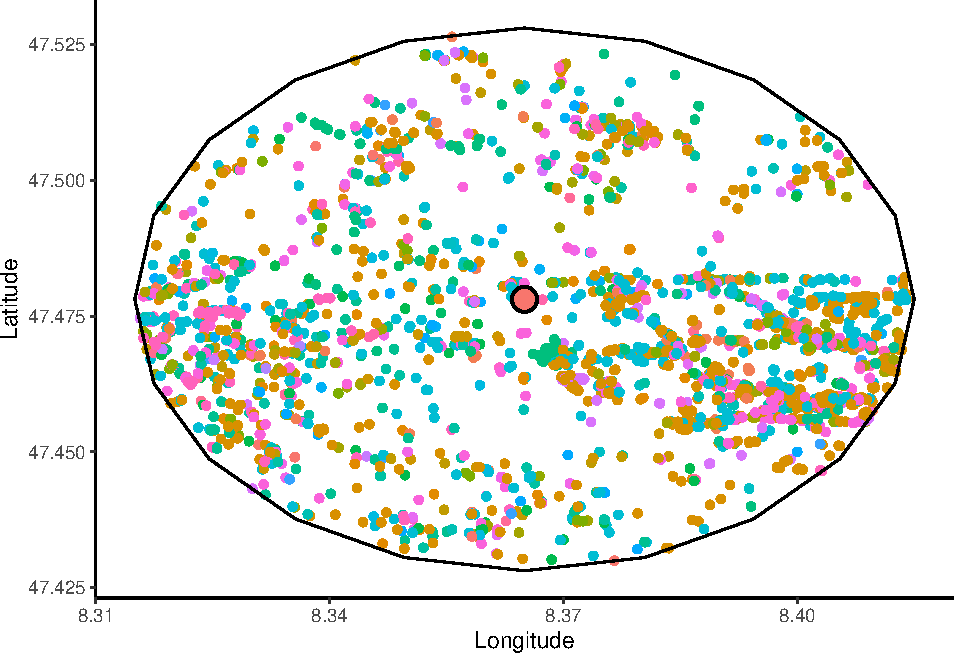
\includegraphics{esds_book_files/figure-latex/unnamed-chunk-74-1.pdf}

To make a species list and calculate the species richness for that tower we simply extract the unique species

\begin{Shaded}
\begin{Highlighting}[]
\NormalTok{sp.list <-}\StringTok{ }\KeywordTok{unique}\NormalTok{(occ_CHlae}\OperatorTok{$}\NormalTok{scientificName)}
\KeywordTok{length}\NormalTok{(}\KeywordTok{unique}\NormalTok{(occ_CHlae}\OperatorTok{$}\NormalTok{scientificName))}
\end{Highlighting}
\end{Shaded}

\begin{verbatim}
## [1] 1254
\end{verbatim}

Normally at this point a species name filtration step would be done. That means the plant names from our species list would be compared to that of `The Plant List' (TPL) using the package \texttt{Taxonstand}.
This is quite time consuming, so we have already done it for the species lists of each tower.
Below is the example code:

\begin{Shaded}
\begin{Highlighting}[]
\CommentTok{# We retrieve name from taxonstand. To specify how much difference in the names we want to allow we specify diffchar=.}
\KeywordTok{library}\NormalTok{(Taxonstand)}
\NormalTok{name <-}\StringTok{ }\KeywordTok{TPL}\NormalTok{(sp.list.final, }\DataTypeTok{diffchar =} \DecValTok{4}\NormalTok{, }\DataTypeTok{drop.lower.level =}\NormalTok{ T)}

\CommentTok{# select columns of interest}
\NormalTok{name <-}\StringTok{ }\NormalTok{name[, }\KeywordTok{c}\NormalTok{(}\StringTok{"Taxon"}\NormalTok{, }\StringTok{"New.Genus"}\NormalTok{, }\StringTok{"New.Species"}\NormalTok{, }\StringTok{"New.Taxonomic.status"}\NormalTok{, }\StringTok{"Typo"}\NormalTok{)]}

\CommentTok{# create column with new species name}
\NormalTok{name}\OperatorTok{$}\NormalTok{autocorrected <-}\StringTok{ }\KeywordTok{paste}\NormalTok{(name}\OperatorTok{$}\NormalTok{New.Genus, name}\OperatorTok{$}\NormalTok{New.Species)}

\CommentTok{# drop new.species and new.genus column}
\NormalTok{name <-}\StringTok{ }\NormalTok{name[, }\KeywordTok{c}\NormalTok{(}\StringTok{"Taxon"}\NormalTok{, }\StringTok{"autocorrected"}\NormalTok{, }\StringTok{"New.Taxonomic.status"}\NormalTok{, }\StringTok{"Typo"}\NormalTok{)]}

\CommentTok{# change column names}
\KeywordTok{colnames}\NormalTok{(name) <-}\StringTok{ }\KeywordTok{c}\NormalTok{(}\StringTok{"submittedname"}\NormalTok{, }\StringTok{"autocorrected"}\NormalTok{, }\StringTok{"taxo_status"}\NormalTok{, }\StringTok{"typo"}\NormalTok{)}

\CommentTok{# Finally, we can drop all species for which we did not find a matching scientific name.}
\NormalTok{names.accepted <-}\StringTok{ }\KeywordTok{unique}\NormalTok{(name[name}\OperatorTok{$}\NormalTok{taxo_status}\OperatorTok{==}\StringTok{"Accepted"}\NormalTok{,])}
\end{Highlighting}
\end{Shaded}

\begin{Shaded}
\begin{Highlighting}[]
\CommentTok{# read in the resolved species names .csv}
\NormalTok{species_list_full <-}\StringTok{ }\KeywordTok{read.csv}\NormalTok{(}\StringTok{"./data/resolved_species_names.csv"}\NormalTok{,}\DataTypeTok{sep=}\StringTok{";"}\NormalTok{)}
\end{Highlighting}
\end{Shaded}

\begin{Shaded}
\begin{Highlighting}[]
\CommentTok{# check how many species are in the list}
\KeywordTok{dim}\NormalTok{(species_list_full)}
\end{Highlighting}
\end{Shaded}

\begin{verbatim}
## [1] 7480    1
\end{verbatim}

Next, we can use this information to build a presence-absence matrix for all locations and species, this will allow us to see where each species is found. This can be the basis for many community ecology calculations or species distribution models linking the environmental variables to species' occurrences to see which are most correlated with certain factors.

\begin{Shaded}
\begin{Highlighting}[]
\CommentTok{# select all files with resolved in their name}
\NormalTok{paths <-}\StringTok{ }\KeywordTok{list.files}\NormalTok{(}\KeywordTok{file.path}\NormalTok{(}\StringTok{"./data/"}\NormalTok{, }\StringTok{"species_occurrences"}\NormalTok{), }\DataTypeTok{pattern=}\StringTok{'resolved_*'}\NormalTok{, }\DataTypeTok{recursive =}\NormalTok{ F, }\DataTypeTok{full.names =}\NormalTok{ T)}

\CommentTok{# create a function to read them all in}
\NormalTok{read_species =}\StringTok{ }\ControlFlowTok{function}\NormalTok{(file_path)\{}
  \KeywordTok{return}\NormalTok{(}\KeywordTok{read.csv}\NormalTok{(file_path,}\DataTypeTok{sep=}\StringTok{";"}\NormalTok{))}
\NormalTok{\}}

\CommentTok{# read all the files in paths in using the function read_species}
\NormalTok{species_occurrences <-}\StringTok{ }\KeywordTok{lapply}\NormalTok{(paths, read_species)}

\CommentTok{# bind them into a df and give an identifier with .id=}
\NormalTok{species_occ_df <-}\StringTok{ }\KeywordTok{bind_rows}\NormalTok{(species_occurrences, }\DataTypeTok{.id=}\StringTok{"id"}\NormalTok{)}

\CommentTok{# make a species occurrence (or presence-absence) matrix}
\NormalTok{species_occ_mat <-}\StringTok{ }\NormalTok{species_occ_df }\OperatorTok
\StringTok{  }\KeywordTok{group_by}\NormalTok{(id)}\OperatorTok\StringTok{                                                                     }\CommentTok{# group the species lists by the sites}
\StringTok{  }\KeywordTok{distinct}\NormalTok{() }\OperatorTok\StringTok{                                                                      }\CommentTok{# select only unique species names since some occur multiple times}
\StringTok{  }\KeywordTok{mutate}\NormalTok{(}\DataTypeTok{present =} \DecValTok{1}\NormalTok{) }\OperatorTok\StringTok{                                                             }\CommentTok{# create a column where all the species get a 1 (for presence)}
\StringTok{  }\KeywordTok{pivot_wider}\NormalTok{(}\DataTypeTok{names_from =}\NormalTok{ names.accepted.autocorrected, }\DataTypeTok{values_from =}\NormalTok{ present) }\OperatorTok\StringTok{   }\CommentTok{# turn (spread) the column of species names to the column names}
\StringTok{  }\KeywordTok{mutate_all}\NormalTok{(}\KeywordTok{funs}\NormalTok{(}\KeywordTok{ifelse}\NormalTok{(}\KeywordTok{is.na}\NormalTok{(.), }\DecValTok{0}\NormalTok{, .)))                                            }\CommentTok{# replace the missing values with 0}
\end{Highlighting}
\end{Shaded}

\begin{Shaded}
\begin{Highlighting}[]
\KeywordTok{head}\NormalTok{(species_occ_mat)}
\end{Highlighting}
\end{Shaded}

\begin{verbatim}
## # A tibble: 6 x 6,651
## # Groups:   id [6]
##   id    `Hedera helix` `Arum italicum` `Asplenium ruta~ `Ceterach offic~
##   <chr>          <dbl>           <dbl>            <dbl>            <dbl>
## 1 1                  1               1                1                1
## 2 2                  1               1                1                1
## 3 3                  1               1                1                1
## 4 4                  1               1                1                1
## 5 5                  1               1                1                1
## 6 6                  1               1                1                1
## # ... with 6,646 more variables: `Artemisia vulgaris` <dbl>, `Corylus
## #   avellana` <dbl>, `Teucrium scorodonia` <dbl>, `Glechoma hederacea` <dbl>,
## #   `Alliaria petiolata` <dbl>, `Plantago lanceolata` <dbl>, `Ficaria
## #   verna` <dbl>, `Trifolium pratense` <dbl>, `Erodium cicutarium` <dbl>,
## #   `Urtica dioica` <dbl>, `Achillea millefolium` <dbl>, `Cirsium
## #   vulgare` <dbl>, `Stellaria media` <dbl>, `Betula pendula` <dbl>,
## #   `Symphoricarpos albus` <dbl>, `Equisetum telmateia` <dbl>, `Euphorbia
## #   peplus` <dbl>, `Aphanes arvensis` <dbl>, `Geranium robertianum` <dbl>,
## #   `Clematis vitalba` <dbl>, `Lamium purpureum` <dbl>, `Lamium album` <dbl>,
## #   `Bellis perennis` <dbl>, `Geum urbanum` <dbl>, `Juncus effusus` <dbl>,
## #   `Chelidonium majus` <dbl>, `Ilex aquifolium` <dbl>, `Daucus carota` <dbl>,
## #   `Lonicera ligustrina` <dbl>, `Senecio vulgaris` <dbl>, `Oxalis
## #   pes-caprae` <dbl>, `Asplenium scolopendrium` <dbl>, `Galium aparine` <dbl>,
## #   `Ranunculus repens` <dbl>, `Calluna vulgaris` <dbl>, `Solanum
## #   dulcamara` <dbl>, `Carex pendula` <dbl>, `Cerastium glomeratum` <dbl>,
## #   `Dipsacus pilosus` <dbl>, `Buddleja davidii` <dbl>, `Pseudosasa
## #   japonica` <dbl>, `Epipactis helleborine` <dbl>, `Lunaria annua` <dbl>,
## #   `Dryopteris carthusiana` <dbl>, `Senecio inaequidens` <dbl>, `Eranthis
## #   hyemalis` <dbl>, `Aesculus hippocastanum` <dbl>, `Geranium molle` <dbl>,
## #   `Polypodium vulgare` <dbl>, `Humulus lupulus` <dbl>, `Arum
## #   maculatum` <dbl>, `Alnus glutinosa` <dbl>, `Tanacetum vulgare` <dbl>,
## #   `Verbascum thapsus` <dbl>, `Capsella bursa-pastoris` <dbl>, `Jasminum
## #   nudiflorum` <dbl>, `Galanthus nivalis` <dbl>, `Acer platanoides` <dbl>,
## #   `Crataegus monogyna` <dbl>, `Pinus sylvestris` <dbl>, `Prunus
## #   laurocerasus` <dbl>, `Quercus robur` <dbl>, `Scrophularia nodosa` <dbl>,
## #   `Erophila verna` <dbl>, `Cardamine hirsuta` <dbl>, `Epilobium
## #   angustifolium` <dbl>, `Rumex obtusifolius` <dbl>, `Anthriscus
## #   sylvestris` <dbl>, `Claytonia perfoliata` <dbl>, `Sonchus oleraceus` <dbl>,
## #   `Cirsium arvense` <dbl>, `Borago officinalis` <dbl>, `Poa annua` <dbl>,
## #   `Alnus rubra` <dbl>, `Viburnum tinus` <dbl>, `Phragmites australis` <dbl>,
## #   `Larix decidua` <dbl>, `Veronica beccabunga` <dbl>, `Lepidium
## #   virginicum` <dbl>, `Mercurialis annua` <dbl>, `Euphorbia
## #   helioscopia` <dbl>, `Cytisus scoparius` <dbl>, `Tripleurospermum
## #   inodorum` <dbl>, `Castanea sativa` <dbl>, `Veronica persica` <dbl>, `Rumex
## #   acetosa` <dbl>, `Sambucus nigra` <dbl>, `Phacelia tanacetifolia` <dbl>,
## #   `Veronica hederifolia` <dbl>, `Taxus baccata` <dbl>, `Silene dioica` <dbl>,
## #   `Asplenium trichomanes` <dbl>, `Oenothera biennis` <dbl>, `Fraxinus
## #   excelsior` <dbl>, `Chenopodium album` <dbl>, `Aucuba japonica` <dbl>,
## #   `Euonymus europaeus` <dbl>, `Taraxacum campylodes` <dbl>, `Solidago
## #   gigantea` <dbl>, `Rhododendron ponticum` <dbl>, ...
\end{verbatim}

GBIF is a great source for species occurrences. However, we have to keep in mind that the data collection is biased by regions. For example, we find much fewer plant records in Africa than in Europe. But also within Europe, there are some biases. Therefore we need to be careful with the interpretation.

\begin{Shaded}
\begin{Highlighting}[]
\NormalTok{nr_occurrences <-}\StringTok{ }\KeywordTok{read_csv}\NormalTok{(}\StringTok{"./data/flx_tower_occurrences.csv"}\NormalTok{)}

\NormalTok{occurrences <-}\StringTok{ }\NormalTok{nr_occurrences}\OperatorTok{$}\NormalTok{nr_occurrences}
\end{Highlighting}
\end{Shaded}

\begin{Shaded}
\begin{Highlighting}[]
\KeywordTok{ggplot}\NormalTok{() }\OperatorTok{+}
\StringTok{  }\KeywordTok{geom_polygon}\NormalTok{(}\DataTypeTok{data =}\NormalTok{ europe_shape,}
               \KeywordTok{aes}\NormalTok{(}\DataTypeTok{x =}\NormalTok{ long, }\DataTypeTok{y =}\NormalTok{ lat, }\DataTypeTok{group =}\NormalTok{ group), }\DataTypeTok{fill =} \OtherTok{NA}\NormalTok{, }\DataTypeTok{colour =} \StringTok{"black"}\NormalTok{) }\OperatorTok{+}
\StringTok{  }\KeywordTok{geom_point}\NormalTok{(}\KeywordTok{aes}\NormalTok{(}\DataTypeTok{colour =}\NormalTok{ occurrences, }\DataTypeTok{x =}\NormalTok{ df_sites}\OperatorTok{$}\NormalTok{lon,}
                              \DataTypeTok{y =}\NormalTok{ df_sites}\OperatorTok{$}\NormalTok{lat)) }\OperatorTok{+}
\StringTok{  }\KeywordTok{scale_colour_gradient}\NormalTok{(}\DataTypeTok{low =} \StringTok{"yellow"}\NormalTok{, }\DataTypeTok{high =} \StringTok{"red"}\NormalTok{, }\DataTypeTok{na.value =} \OtherTok{NA}\NormalTok{) }\OperatorTok{+}
\StringTok{  }\KeywordTok{theme_classic}\NormalTok{() }\OperatorTok{+}\StringTok{ }\KeywordTok{xlab}\NormalTok{(}\StringTok{"Longitude"}\NormalTok{) }\OperatorTok{+}\StringTok{ }\KeywordTok{ylab}\NormalTok{(}\StringTok{"Latitude"}\NormalTok{) }\OperatorTok{+}\StringTok{ }\KeywordTok{coord_quickmap}\NormalTok{()}
\end{Highlighting}
\end{Shaded}

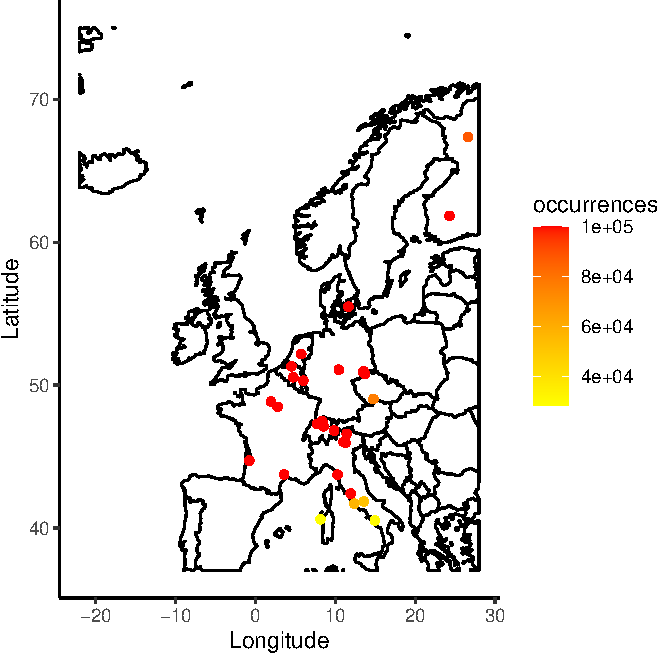
\includegraphics{esds_book_files/figure-latex/unnamed-chunk-83-1.pdf}

We see that the numbers of occurrence records in southern Europe are lower than in central Europe. This suggests there is a sampling bias, with a higher sampling effort in central European countries.

Knowing the species richness of the different sites can help us learn more about the ecological context the towers are located in. We made the occurrence matrix above and now we'll use that to plot the richness. The richness is the number of species at each site. Since each row in the matrix is a site we can just sum the rows and we'll get the number of species per site. We don't have data for all our towers in \emph{df\_sites} so we will make a new dataframe with only the relevant sites and call it \emph{df\_sp\_sites}.

\begin{Shaded}
\begin{Highlighting}[]
\CommentTok{# remove the sites for which we have no species lists}
\NormalTok{df_sp_sites <-}\StringTok{ }\NormalTok{df_sites }\OperatorTok\StringTok{ }
\StringTok{  }\KeywordTok{filter}\NormalTok{(}\OperatorTok{!}\NormalTok{(site }\OperatorTok\StringTok{ }\KeywordTok{c}\NormalTok{(}\StringTok{"CH-Oe1"}\NormalTok{, }\StringTok{"DE-Obe"}\NormalTok{, }\StringTok{"FR-LBr"}\NormalTok{, }\StringTok{"IT-Cpz"}\NormalTok{, }\StringTok{"IT-Ro1"}\NormalTok{)))}

\CommentTok{# the first column is the 'id', so we exclude that}
\NormalTok{richness <-}\StringTok{ }\KeywordTok{rowSums}\NormalTok{(species_occ_mat[,}\OperatorTok{-}\DecValTok{1}\NormalTok{])}

\KeywordTok{ggplot}\NormalTok{() }\OperatorTok{+}
\StringTok{  }\KeywordTok{geom_polygon}\NormalTok{(}\DataTypeTok{data =}\NormalTok{ europe_shape,}
               \KeywordTok{aes}\NormalTok{(}\DataTypeTok{x =}\NormalTok{ long, }\DataTypeTok{y =}\NormalTok{ lat, }\DataTypeTok{group =}\NormalTok{ group), }\DataTypeTok{fill =} \OtherTok{NA}\NormalTok{, }\DataTypeTok{colour =} \StringTok{"black"}\NormalTok{) }\OperatorTok{+}
\StringTok{  }\KeywordTok{geom_point}\NormalTok{(}\KeywordTok{aes}\NormalTok{(}\DataTypeTok{colour =}\NormalTok{ richness, }\DataTypeTok{x =}\NormalTok{ df_sp_sites}\OperatorTok{$}\NormalTok{lon,}
                              \DataTypeTok{y =}\NormalTok{ df_sp_sites}\OperatorTok{$}\NormalTok{lat)) }\OperatorTok{+}
\StringTok{  }\KeywordTok{scale_colour_gradient}\NormalTok{(}\DataTypeTok{low =} \StringTok{"yellow"}\NormalTok{, }\DataTypeTok{high =} \StringTok{"red"}\NormalTok{, }\DataTypeTok{na.value =} \OtherTok{NA}\NormalTok{) }\OperatorTok{+}
\StringTok{  }\KeywordTok{theme_classic}\NormalTok{() }\OperatorTok{+}\StringTok{ }\KeywordTok{xlab}\NormalTok{(}\StringTok{"Longitude"}\NormalTok{) }\OperatorTok{+}\StringTok{ }\KeywordTok{ylab}\NormalTok{(}\StringTok{"Latitude"}\NormalTok{) }\OperatorTok{+}\StringTok{ }\KeywordTok{coord_quickmap}\NormalTok{()}
\end{Highlighting}
\end{Shaded}

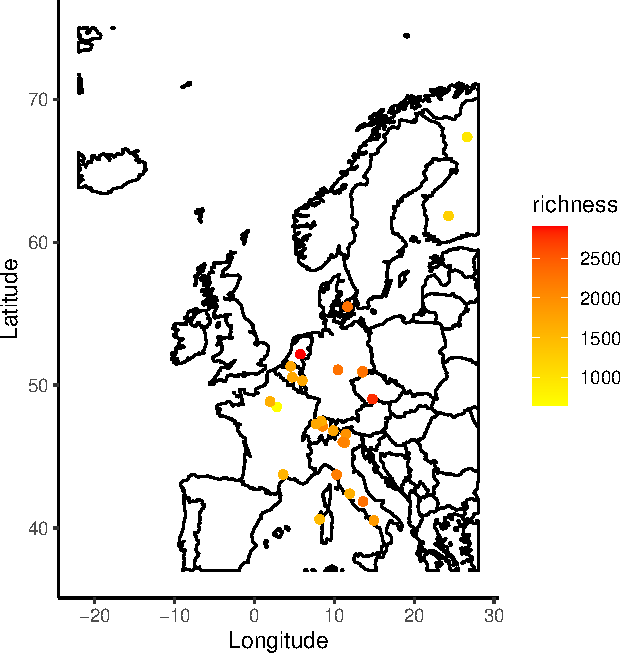
\includegraphics{esds_book_files/figure-latex/unnamed-chunk-84-1.pdf}

\hypertarget{species-traits}{%
\subsubsection{Species Traits}\label{species-traits}}

In the next step, we will study the relationship between plant traits, GPP, and climatic variables for our fluxnet towers. We obtained data from the TRY database, which is a database containing plant trait data. You can make data requests on \href{www.https://www.try-db.org}{their website}. You can select the traits that you are interested in and the species for which you would like to look at the traits.
For this tutorial we already requested a dataset, because usually, it takes time to receive the data. We downloaded data on 9 different traits for all species available. We extracted the trait data for all the species we have in our species list (and therefore also in our species occurrence matrix).

Let's load the data.

\begin{Shaded}
\begin{Highlighting}[]
\NormalTok{trait_df <-}\StringTok{ }\KeywordTok{read.csv}\NormalTok{(}\StringTok{"./data/Trait_df.csv"}\NormalTok{)}
\KeywordTok{head}\NormalTok{(trait_df)}
\end{Highlighting}
\end{Shaded}

\begin{verbatim}
##   X.1 X         SpeciesName
## 1   1 1      Acer campestre
## 2   2 2      Acer campestre
## 3   3 3 Acer pseudoplatanus
## 4   4 4 Acer pseudoplatanus
## 5   5 5     Alnus glutinosa
## 6   6 6     Alnus glutinosa
##                                                   TraitName TraitID
## 1                                            Leaf thickness      46
## 2 Leaf texture (sclerophylly, physical strength, toughness)       2
## 3                                            Leaf thickness      46
## 4 Leaf texture (sclerophylly, physical strength, toughness)       2
## 5                                            Leaf thickness      46
## 6 Leaf texture (sclerophylly, physical strength, toughness)       2
##   OrigValueStr OrigUnitStr OrigUncertaintyStr UncertaintyName
## 1   0.14400000          mm         0.00400000  Standard Error
## 2   0.04511078   (N/10)/mm         0.01426528  Standard Error
## 3   0.17800000          mm         0.01655295  Standard Error
## 4   0.06038498   (N/10)/mm         0.01909541  Standard Error
## 5   0.13600000          mm         0.00509902  Standard Error
## 6   0.06667092   (N/10)/mm         0.02108320  Standard Error
\end{verbatim}

Some examples of traits are are leaf texture, leaf thickness, eaf chlorophyll content per leaf area, specific leaf area, etc.

As a next step, we can combine the species occurrence data with the trait data. The presence/absence matrix (\emph{species\_occ\_mat}) we made earlier, gives us the species present at each site. From that we can then extract these species and their respective trait values from the trait dataframe (\emph{trait\_df}). Then we go on to summarise this data by calculating the mean value for each trait across all the species at the tower sites.

We start by doing this for one site.

\begin{Shaded}
\begin{Highlighting}[]
\NormalTok{ba <-}\StringTok{ }\NormalTok{trait_df}

\CommentTok{# select all the species (species names= column names) which are present (so ==1)}
\NormalTok{species_present <-}\StringTok{ }\KeywordTok{colnames}\NormalTok{(species_occ_mat)[}\KeywordTok{which}\NormalTok{(species_occ_mat[}\DecValTok{1}\NormalTok{, ] }\OperatorTok{==}\StringTok{ }\DecValTok{1}\NormalTok{)]}

\CommentTok{# filter out the trait data for the species present at that site}
\NormalTok{trait_subset <-}\StringTok{ }\NormalTok{ba[ba}\OperatorTok{$}\NormalTok{SpeciesName }\OperatorTok\StringTok{ }\NormalTok{species_present,]}

\CommentTok{# calculate the mean of each trait across all species present}
\NormalTok{bac <-}\StringTok{ }\KeywordTok{aggregate}\NormalTok{(trait_subset}\OperatorTok{$}\NormalTok{OrigValueStr, }\KeywordTok{list}\NormalTok{(trait_subset}\OperatorTok{$}\NormalTok{TraitID), mean, }\DataTypeTok{na.rm=}\NormalTok{T)}
\end{Highlighting}
\end{Shaded}

To finish preparing the data for the PCA, we do the above steps for all the remaining sites by using a \emph{`for loop'}.

\begin{Shaded}
\begin{Highlighting}[]
\NormalTok{df_pca <-}\StringTok{ }\NormalTok{bac}\OperatorTok{$}\NormalTok{x}
\ControlFlowTok{for}\NormalTok{(i }\ControlFlowTok{in} \KeywordTok{c}\NormalTok{(}\DecValTok{2}\OperatorTok{:}\DecValTok{28}\NormalTok{))\{}
\NormalTok{    species_present <-}\StringTok{ }\KeywordTok{colnames}\NormalTok{(species_occ_mat)[}\KeywordTok{which}\NormalTok{(species_occ_mat[i, ] }\OperatorTok{==}\StringTok{ }\DecValTok{1}\NormalTok{)]}
\NormalTok{    trait_subset <-}\StringTok{ }\NormalTok{ba[ba}\OperatorTok{$}\NormalTok{SpeciesName }\OperatorTok\StringTok{ }\NormalTok{species_present,]}
\NormalTok{    bac <-}\StringTok{ }\KeywordTok{aggregate}\NormalTok{(trait_subset}\OperatorTok{$}\NormalTok{OrigValueStr, }\KeywordTok{list}\NormalTok{(trait_subset}\OperatorTok{$}\NormalTok{TraitID), mean, }\DataTypeTok{na.rm=}\NormalTok{T)}
\NormalTok{    df_pca <-}\StringTok{ }\KeywordTok{rbind}\NormalTok{(df_pca, bac}\OperatorTok{$}\NormalTok{x)}
\NormalTok{\}}
\end{Highlighting}
\end{Shaded}

For the PCA we use only the traits with traitIDs: 46, 47, 3106 and 3117. This is because the other traits are just slightly modified versions of these four traits. These four traitIDs correspond to the traits: \emph{leaf thickness}, \emph{leaf dry matter content (LDMC)}, \emph{plant height} and \emph{specific leaf area (SLA)}. \emph{Leaf dry matter content} is calculated as leaf dry mass per leaf fresh mass and \emph{specific leaf area} is defined as leaf area per leaf dry mass.

\begin{Shaded}
\begin{Highlighting}[]
\CommentTok{# we select the columns corresponding to our desired traits}
\NormalTok{df_pca <-}\StringTok{ }\KeywordTok{cbind}\NormalTok{(df_pca[,}\DecValTok{2}\NormalTok{],df_pca[,}\DecValTok{3}\NormalTok{],df_pca[,}\DecValTok{5}\NormalTok{],df_pca[,}\DecValTok{9}\NormalTok{])}

\CommentTok{# to make the data easier to understand we name the columns after the trait}
\KeywordTok{colnames}\NormalTok{(df_pca) <-}\StringTok{ }\KeywordTok{c}\NormalTok{(}\StringTok{"leaf thickness"}\NormalTok{, }\StringTok{"leaf dry matter content (LDMC)"}\NormalTok{, }\StringTok{"plant height vegetative"}\NormalTok{, }\StringTok{"specific leaf area (SLA)"}\NormalTok{)}

\KeywordTok{head}\NormalTok{(df_pca)}
\end{Highlighting}
\end{Shaded}

\begin{verbatim}
##        leaf thickness leaf dry matter content (LDMC) plant height vegetative
## df_pca       18.38967                       142.1853                80.59372
##              19.11832                       144.8715                80.23070
##              19.32090                       176.7112                80.68073
##              21.47128                       144.4585                73.76227
##              22.30091                       148.8697                70.61044
##              22.17279                       144.7945                73.61253
##        specific leaf area (SLA)
## df_pca                 77.28056
##                        78.31965
##                        81.82512
##                        78.28065
##                        76.57826
##                        76.61992
\end{verbatim}

Principal Component Analysis (PCA) is one of famous techniques for dimension reduction, feature extraction, and data visualization. In general, PCA is defined as the transformation of a high dimensional vector space to a low dimensional space. Just imagine having to visualise data with 10 dimensions\ldots{} we often stuggle already with three. It's almost impossible to effectively show the shape of such a high dimensional data distribution. PCA provides an efficient way to reduce the dimensionalty (i.e.~from 10 to 2), so it is much easier to visualize the shape of data distribution. In a nutshell, this reduction happens by the PCA taking the two axes that best explain the variation in the data.

PCA is also useful in the modeling a robust classifier where considerably small number of high dimensional training data is provided. By reducing the dimensions of learning data sets, PCA provides an effective and efficient method for data description and classification.
For a more mathematical description of PCA you can check \url{https://www.projectrhea.org/rhea/index.php/PCA_Theory_Examples}.

So now let's reduce the dimensions of our trait data as an example\ldots{} For this we use the function \texttt{prcomp()}.

\begin{Shaded}
\begin{Highlighting}[]
\NormalTok{traits_pca <-}\StringTok{ }\KeywordTok{prcomp}\NormalTok{(df_pca, }\DataTypeTok{center =} \OtherTok{TRUE}\NormalTok{, }\DataTypeTok{scale =} \OtherTok{TRUE}\NormalTok{)}
\KeywordTok{summary}\NormalTok{(traits_pca)}
\end{Highlighting}
\end{Shaded}

\begin{verbatim}
## Importance of components:
##                           PC1    PC2    PC3     PC4
## Standard deviation     1.5372 0.9280 0.6972 0.53830
## Proportion of Variance 0.5907 0.2153 0.1215 0.07244
## Cumulative Proportion  0.5907 0.8060 0.9276 1.00000
\end{verbatim}

From the information above we can see how much of the variation in the data is explained by each axis or dimensionality. Ideally, you want the first to axes to explain the vast majority of the variation, while the subsequent ones are much less important.
But what do all these numbers mean and how does the data look. It's time to visualise the PCA.

\begin{Shaded}
\begin{Highlighting}[]
\KeywordTok{library}\NormalTok{(ggfortify)}
\KeywordTok{autoplot}\NormalTok{(traits_pca, }\DataTypeTok{data =}\NormalTok{ df_pca, }\DataTypeTok{col =}\StringTok{"#138D37"}\NormalTok{, }\DataTypeTok{loadings =} \OtherTok{TRUE}\NormalTok{, }\DataTypeTok{loadings.colour =} \StringTok{'blue'}\NormalTok{, }\DataTypeTok{loadings.label =} \OtherTok{TRUE}\NormalTok{, }\DataTypeTok{loadings.label.size =} \DecValTok{3}\NormalTok{) }\OperatorTok{+}\StringTok{ }\KeywordTok{theme_classic}\NormalTok{()}
\end{Highlighting}
\end{Shaded}

\begin{verbatim}
## Warning: `select_()` is deprecated as of dplyr 0.7.0.
## Please use `select()` instead.
## This warning is displayed once every 8 hours.
## Call `lifecycle::last_warnings()` to see where this warning was generated.
\end{verbatim}

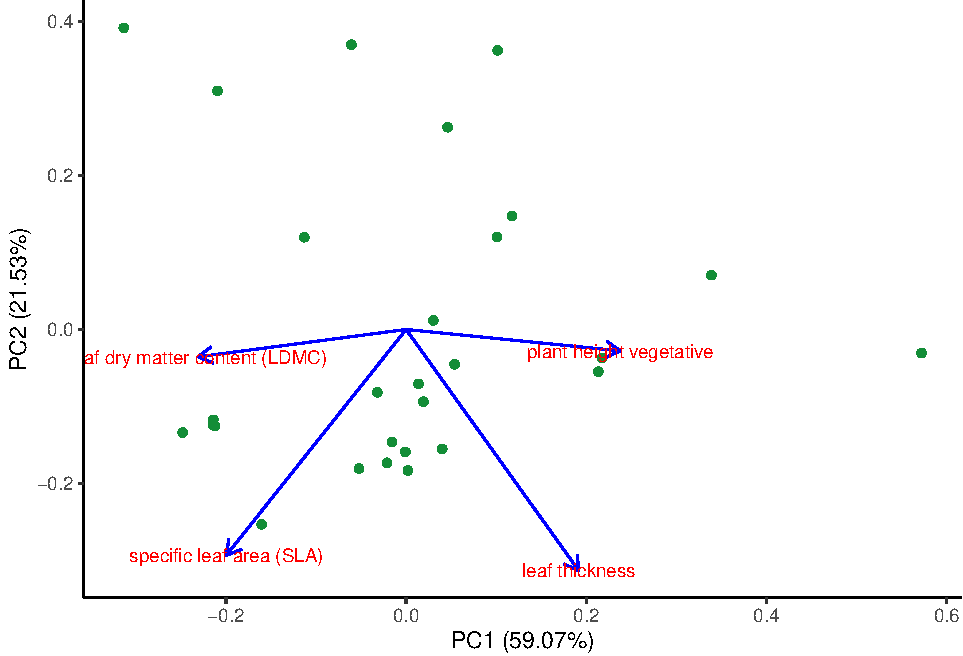
\includegraphics{esds_book_files/figure-latex/unnamed-chunk-90-1.pdf}

We have successfully reduced the dimensionality of our data! We started with four traits and now we have reduced the variation to two main axes. We see that PC1 is mainly associated to leaf dry matter content, and plant height, while PC2 is associated with specific leaf area and leaf thickness.

It can be interesting to see how the points relate spatially, this could, for example, allow us to identify clusters. Therefore, we will visualise our tower sites coloured by the corresponding position (positive or negative) on the PC1 axes.

\begin{Shaded}
\begin{Highlighting}[]
\CommentTok{# start by designating trait and axis values to vector objects}
\NormalTok{tr1 <-}\StringTok{ }\NormalTok{df_pca[,}\DecValTok{1}\NormalTok{] }\CommentTok{# these are the traits}
\NormalTok{tr2 <-}\StringTok{ }\NormalTok{df_pca[,}\DecValTok{2}\NormalTok{] }\CommentTok{# these are the traits}

\NormalTok{pc1 <-}\StringTok{ }\NormalTok{traits_pca}\OperatorTok{$}\NormalTok{x[,}\DecValTok{1}\NormalTok{] }\CommentTok{# these are the axis values}
\NormalTok{pc2 <-}\StringTok{ }\NormalTok{traits_pca}\OperatorTok{$}\NormalTok{x[,}\DecValTok{2}\NormalTok{] }\CommentTok{# these are the axis values}
\end{Highlighting}
\end{Shaded}

\begin{Shaded}
\begin{Highlighting}[]
\CommentTok{# specify the colour palettes for positive and negative values}
\NormalTok{pospal <-}\StringTok{ }\KeywordTok{colorRampPalette}\NormalTok{(}\KeywordTok{c}\NormalTok{(}\StringTok{"#E9E15C"}\NormalTok{, }\StringTok{"#CF2B1E"}\NormalTok{))}
\NormalTok{negpal <-}\StringTok{ }\KeywordTok{colorRampPalette}\NormalTok{(}\KeywordTok{c}\NormalTok{(}\StringTok{"#1E3498"}\NormalTok{, }\StringTok{"#95D7DB"}\NormalTok{))}

\CommentTok{# we separate positive from negative values for visualization}
\NormalTok{neg_pc1 <-}\StringTok{ }\NormalTok{pc1 }
\NormalTok{neg_pc1[neg_pc1 }\OperatorTok{>}\StringTok{ }\DecValTok{0}\NormalTok{ ] <-}\StringTok{ }\OtherTok{NA}
\NormalTok{pos_pc1 <-}\StringTok{ }\NormalTok{pc1 }
\NormalTok{pos_pc1[pos_pc1 }\OperatorTok{<}\StringTok{ }\DecValTok{0}\NormalTok{ ] <-}\StringTok{ }\OtherTok{NA}

\NormalTok{datColpos <-}\StringTok{ }\KeywordTok{pospal}\NormalTok{(}\DecValTok{100}\NormalTok{)[}\KeywordTok{as.numeric}\NormalTok{(}\KeywordTok{cut}\NormalTok{(pos_pc1,}\DataTypeTok{breaks =} \DecValTok{100}\NormalTok{))] }
\NormalTok{datColneg <-}\StringTok{ }\KeywordTok{negpal}\NormalTok{(}\DecValTok{100}\NormalTok{)[}\KeywordTok{as.numeric}\NormalTok{(}\KeywordTok{cut}\NormalTok{(neg_pc1,}\DataTypeTok{breaks =} \DecValTok{100}\NormalTok{))]}
\end{Highlighting}
\end{Shaded}

Once the colours are defined, we can plot PC1.

\begin{Shaded}
\begin{Highlighting}[]
\CommentTok{#PC1 }
\KeywordTok{plot}\NormalTok{(europe_shape)}
\KeywordTok{points}\NormalTok{(df_sp_sites}\OperatorTok{$}\NormalTok{lon, df_sp_sites}\OperatorTok{$}\NormalTok{lat, }\DataTypeTok{col=}\NormalTok{datColpos,}\DataTypeTok{cex=}\DecValTok{1}\NormalTok{, }\DataTypeTok{pch =} \DecValTok{19}\NormalTok{) }
\KeywordTok{points}\NormalTok{(df_sp_sites}\OperatorTok{$}\NormalTok{lon, df_sp_sites}\OperatorTok{$}\NormalTok{lat, }\DataTypeTok{col=}\NormalTok{datColneg,}\DataTypeTok{cex=}\DecValTok{1}\NormalTok{, }\DataTypeTok{pch =} \DecValTok{19}\NormalTok{)}
\end{Highlighting}
\end{Shaded}

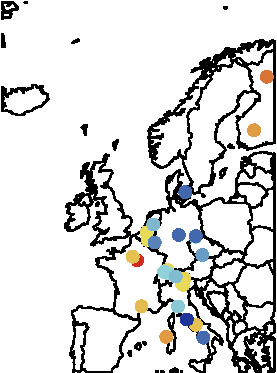
\includegraphics{esds_book_files/figure-latex/unnamed-chunk-93-1.pdf}

And then repeat the process for PC2:

\begin{Shaded}
\begin{Highlighting}[]
\CommentTok{# PC2}
\NormalTok{neg_pc2 <-}\StringTok{ }\NormalTok{pc2 }
\NormalTok{neg_pc2[neg_pc2 }\OperatorTok{>}\StringTok{ }\DecValTok{0}\NormalTok{ ] <-}\StringTok{ }\OtherTok{NA}
\NormalTok{pos_pc2 <-}\StringTok{ }\NormalTok{pc2 }
\NormalTok{pos_pc2[pos_pc2 }\OperatorTok{<}\StringTok{ }\DecValTok{0}\NormalTok{ ] <-}\StringTok{ }\OtherTok{NA}

\NormalTok{datColpos <-}\StringTok{ }\KeywordTok{pospal}\NormalTok{(}\DecValTok{100}\NormalTok{)[}\KeywordTok{as.numeric}\NormalTok{(}\KeywordTok{cut}\NormalTok{(pos_pc2,}\DataTypeTok{breaks =} \DecValTok{100}\NormalTok{))] }
\NormalTok{datColneg <-}\StringTok{ }\KeywordTok{negpal}\NormalTok{(}\DecValTok{100}\NormalTok{)[}\KeywordTok{as.numeric}\NormalTok{(}\KeywordTok{cut}\NormalTok{(neg_pc2,}\DataTypeTok{breaks =} \DecValTok{100}\NormalTok{))]}

\CommentTok{# and plot it on the map}
\KeywordTok{plot}\NormalTok{(europe_shape)}
\KeywordTok{points}\NormalTok{(df_sp_sites}\OperatorTok{$}\NormalTok{lon, df_sp_sites}\OperatorTok{$}\NormalTok{lat, }\DataTypeTok{col=}\NormalTok{datColpos,}\DataTypeTok{cex=}\DecValTok{1}\NormalTok{, }\DataTypeTok{pch =} \DecValTok{19}\NormalTok{)}
\KeywordTok{points}\NormalTok{(df_sp_sites}\OperatorTok{$}\NormalTok{lon, df_sp_sites}\OperatorTok{$}\NormalTok{lat, }\DataTypeTok{col=}\NormalTok{datColneg,}\DataTypeTok{cex=}\DecValTok{1}\NormalTok{, }\DataTypeTok{pch =} \DecValTok{19}\NormalTok{)}
\end{Highlighting}
\end{Shaded}

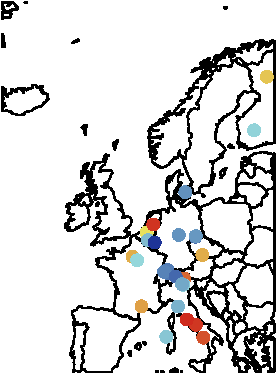
\includegraphics{esds_book_files/figure-latex/unnamed-chunk-94-1.pdf}

The last step in our trait data PCA is to compare the results with GPP. Since GPP has more sites than we used for this analysis we start by removing these sites.

\begin{Shaded}
\begin{Highlighting}[]
\NormalTok{GPP_pca <-}\StringTok{ }\NormalTok{GPP }\OperatorTok\StringTok{ }
\StringTok{  }\KeywordTok{filter}\NormalTok{(}\OperatorTok{!}\NormalTok{(siteid }\OperatorTok\StringTok{ }\KeywordTok{c}\NormalTok{(}\StringTok{"CH-Oe1"}\NormalTok{, }\StringTok{"DE-Obe"}\NormalTok{, }\StringTok{"FR-LBr"}\NormalTok{, }\StringTok{"IT-Cpz"}\NormalTok{, }\StringTok{"IT-Ro1"}\NormalTok{)))}
\end{Highlighting}
\end{Shaded}

Then we make a linear model for PC1 and GPP and plot it.

\begin{Shaded}
\begin{Highlighting}[]
\NormalTok{reg_gpp_pc1 <-}\StringTok{ }\KeywordTok{lm}\NormalTok{(gpp_meanann}\OperatorTok{~}\NormalTok{pc1, }\DataTypeTok{data =}\NormalTok{ GPP_pca)}

\NormalTok{GPP_pca }\OperatorTok\StringTok{ }
\StringTok{  }\KeywordTok{ggplot}\NormalTok{(}\KeywordTok{aes}\NormalTok{(}\DataTypeTok{x =}\NormalTok{ pc1, }\DataTypeTok{y =}\NormalTok{ gpp_meanann)) }\OperatorTok{+}
\StringTok{  }\KeywordTok{geom_point}\NormalTok{() }\OperatorTok{+}
\StringTok{  }\KeywordTok{geom_smooth}\NormalTok{(}\DataTypeTok{method=}\StringTok{'lm'}\NormalTok{, }\DataTypeTok{color=}\StringTok{"red"}\NormalTok{, }\DataTypeTok{size=}\FloatTok{0.5}\NormalTok{, }\DataTypeTok{se=}\OtherTok{FALSE}\NormalTok{) }\OperatorTok{+}
\StringTok{  }\KeywordTok{xlab}\NormalTok{(}\StringTok{"PC1"}\NormalTok{) }\OperatorTok{+}
\StringTok{  }\KeywordTok{ylab}\NormalTok{(}\StringTok{"GPP mean [µmolCO2 m-2 s-1]"}\NormalTok{) }\OperatorTok{+}
\StringTok{  }\KeywordTok{theme_classic}\NormalTok{()}
\end{Highlighting}
\end{Shaded}

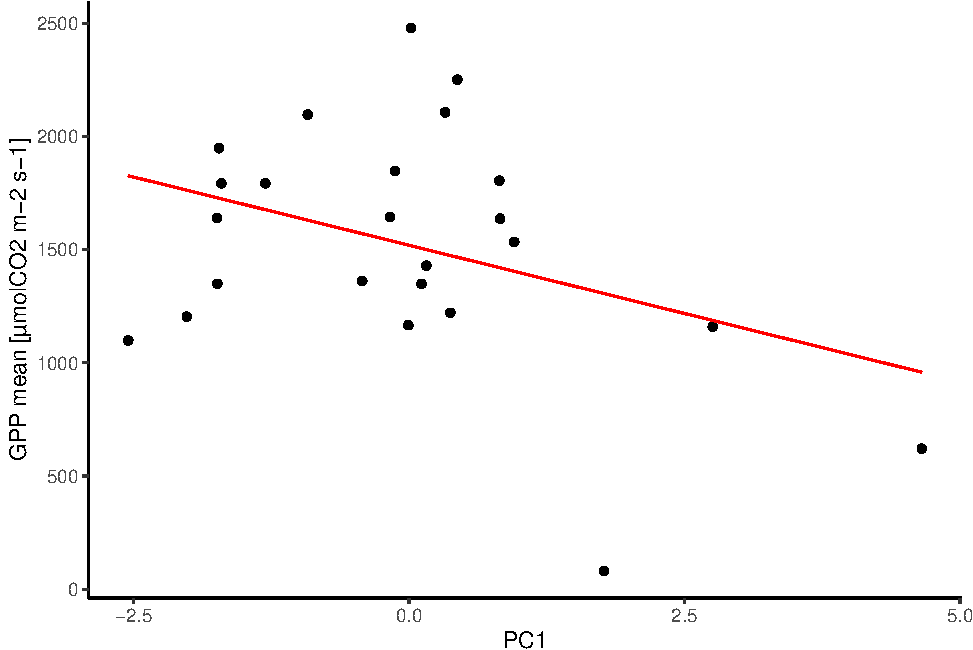
\includegraphics{esds_book_files/figure-latex/unnamed-chunk-96-1.pdf}

We repeat this for GPP and PC2.

\begin{Shaded}
\begin{Highlighting}[]
\NormalTok{reg_gpp_pc2 <-}\StringTok{ }\KeywordTok{lm}\NormalTok{(gpp_meanann}\OperatorTok{~}\NormalTok{pc2, }\DataTypeTok{data =}\NormalTok{ GPP_pca)}

\NormalTok{GPP_pca }\OperatorTok\StringTok{ }
\StringTok{  }\KeywordTok{ggplot}\NormalTok{(}\KeywordTok{aes}\NormalTok{(}\DataTypeTok{x =}\NormalTok{ pc2, }\DataTypeTok{y =}\NormalTok{ gpp_meanann)) }\OperatorTok{+}
\StringTok{  }\KeywordTok{geom_point}\NormalTok{() }\OperatorTok{+}
\StringTok{  }\KeywordTok{geom_smooth}\NormalTok{(}\DataTypeTok{method=}\StringTok{'lm'}\NormalTok{, }\DataTypeTok{color=}\StringTok{"red"}\NormalTok{, }\DataTypeTok{size=}\FloatTok{0.5}\NormalTok{, }\DataTypeTok{se=}\OtherTok{FALSE}\NormalTok{) }\OperatorTok{+}
\StringTok{  }\KeywordTok{xlab}\NormalTok{(}\StringTok{"PC2"}\NormalTok{) }\OperatorTok{+}
\StringTok{  }\KeywordTok{ylab}\NormalTok{(}\StringTok{"GPP mean [µmolCO2 m-2 s-1]"}\NormalTok{) }\OperatorTok{+}
\StringTok{  }\KeywordTok{theme_classic}\NormalTok{() }
\end{Highlighting}
\end{Shaded}

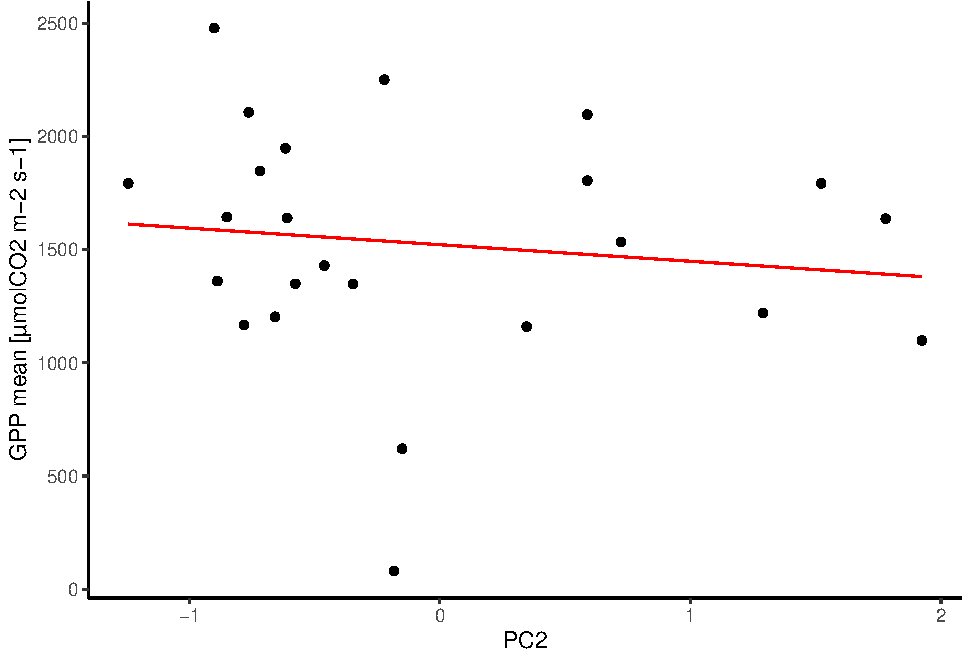
\includegraphics{esds_book_files/figure-latex/unnamed-chunk-97-1.pdf}

Once again we see weak correlations with GPP. Therefore, we can conclude that this further search for predictors that explain the variation in GPP has not yielded any good results. We will have to continue looking for better predictors, which explain this variation in GPP between the sites.

\textbf{Checkpoint}

Plot the spatial distribution of the trait `leaf thickness', make the colour or size related to the leaf thickness values. Describe what you can gather from this plot.

\textbf{Solution}

\begin{Shaded}
\begin{Highlighting}[]
\NormalTok{leaf_t <-}\StringTok{ }\NormalTok{df_pca[,}\DecValTok{1}\NormalTok{]}

\NormalTok{leavepal <-}\StringTok{ }\KeywordTok{colorRampPalette}\NormalTok{(}\KeywordTok{c}\NormalTok{(}\StringTok{"#E2C151"}\NormalTok{,}\StringTok{"#138D37"}\NormalTok{))}

\NormalTok{datColleaves <-}\StringTok{ }\KeywordTok{leavepal}\NormalTok{(}\DecValTok{10}\NormalTok{)[}\KeywordTok{as.numeric}\NormalTok{(}\KeywordTok{cut}\NormalTok{(leaf_t,}\DataTypeTok{breaks =} \DecValTok{10}\NormalTok{))]}

\KeywordTok{plot}\NormalTok{(europe_shape)}
\KeywordTok{points}\NormalTok{(df_sp_sites}\OperatorTok{$}\NormalTok{lon, df_sp_sites}\OperatorTok{$}\NormalTok{lat, }\DataTypeTok{col=}\NormalTok{datColleaves,}\DataTypeTok{cex=}\NormalTok{leaf_t}\OperatorTok{/}\DecValTok{18}\NormalTok{, }\DataTypeTok{pch =} \DecValTok{19}\NormalTok{) }
\end{Highlighting}
\end{Shaded}

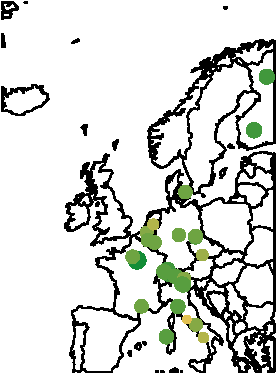
\includegraphics{esds_book_files/figure-latex/unnamed-chunk-98-1.pdf}

The distribution of leaf thickness seems to depend on latitude. In Southern regions, leaves are generally thinner than in Northern regions. To confirm this we would have to make a model and test our observation.

\hypertarget{data-scraping}{%
\chapter{Data Scraping}\label{data-scraping}}

\begin{center}\rule{0.5\linewidth}{0.5pt}\end{center}

\hypertarget{introduction-1}{%
\section{Introduction}\label{introduction-1}}

This chapter covers \emph{data scraping} in R and yes, this is not a typo. \emph{Scraping} means to gather or to extract whereas \emph{scrapping} means to get rid of something. The goal of the sections below is to gather and convert online data into a structured format that can be easily accessed and modified in R. As a case study, we will scrape data from a website containing various information about fish species, called \href{https://www.fishbase.in/search.php}{FishBase}.

We will first learn how to access the website and how to extract useful useful information from plain text. Then, we will look at how to access a table that is embedded in the website and how to generate a new table in R which holds all information we want to extract. Next up is cleaning up the scraped data for visualization and analysis. At the end we will conduct a case study where we create a model to make predictions about fish species richness.

\begin{center}\rule{0.5\linewidth}{0.5pt}\end{center}

\hypertarget{theory}{%
\section{Theory}\label{theory}}

Let us first have a brief review of the main concept of the lecture. The web is the largest source of information and often free to access. In some cases the information is already presented in a nice format and can be easily copied into an excel spreadsheet. However, this is often not the case and data-sets are only presented in a format that is not easy to download or modify. Manually copying data from different sub pages and sections is a tedious, slow and error prone approach. We therefore need a more automated and efficient technique to access such data.

Web scraping is a popular technique to extract information directly from a website by accessing its underlying HTML code. Scraping allows us to gather this unstructured data from many websites and put it all together in a ready-to-use data format. This structured data can then be further used as training, validation or test data sets for our machine learning algorithms.

\textbf{Important Concepts of Websites}

\begin{itemize}
\item
  \textbf{HTTP}: The \textbf{H}yper\textbf{t}ext \textbf{T}ransfer \textbf{P}rotocol is a widely used protocol for information systems. Hypertext documents include hyperlinks that can be clicked to access other resources. Put simply, HTTP is the foundation of how information, i.e., data, is communicated in the world wide web.
\item
  \textbf{HTML}: \textbf{H}yper\textbf{t}ext \textbf{M}arkup \textbf{L}anguage is the coding language in which most websites are written. This includes elements like formatting or structuring and is often combined using CSS or JavaScript. HTML is organized using tags, which are surrounded by \texttt{\textless{}\ \textgreater{}}. Each HTML document is made of elements that are specified using tags. HTML elements and HTML tags are often confused. Tags are used to open and close the object, whereas elements include both tags and its content.

  Let's consider an example with the \texttt{\textless{}h1\textgreater{}} tag: \texttt{\textless{}h1\textgreater{}\ Title\ of\ the\ document\ \textless{}/h1\textgreater{}} is an element, and \texttt{\textless{}h1\textgreater{}}, \texttt{\textless{}/h1\textgreater{}} - are the tags enclosing it. The \texttt{\textless{}\textgreater{}} symbol is used to open a tag or an element and \texttt{\textless{}/\textgreater{}} is used to close it. HTML documents have a hierarchical or tree like structure with different types of nodes as described in \ref{fig:node-tree}. The rectangular boxes are referred to as nodes. The \emph{Text} node is also called as a child node of the \emph{Element} node and also a leaf node as it only contains text and no links to further nodes. Both of the \emph{Element} nodes that are attached to the \emph{Root Element} node are called sibling nodes of the \emph{Root Element} node. When we do web scraping we go through such a hierarchical structure to get the content (here text in the \emph{Test} node). Keep in mind that every HTML document can vary with respect to its structure. This example is to just to provide you some knowledge about HTML document and its structure.
\end{itemize}

\begin{figure}
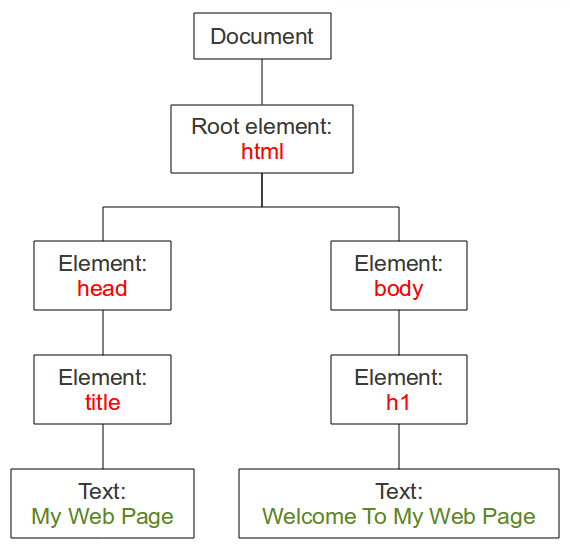
\includegraphics[width=7.92in]{./figures/node-tree} \caption{Visualization of the structure of an HTML document.}\label{fig:node-tree}
\end{figure}

\begin{itemize}
\item
  \textbf{XML}: The E\textbf{x}tensible \textbf{M}arkup \textbf{L}anguage has some similarities to HTML but the format is generally easier to read for machines. While HTML has a number of pre-defined tags, one can create (``extend'') new tags as needed . This allows to define and control the meaning of the elements contained in a document or text.
\item
  \textbf{API}: An \textbf{A}pplication \textbf{P}rogramming \textbf{I}nterface is a set of procedures and communication protocols that provide access to the data of an application, operating system or other services. Both APIs and web scraping are used to retrieve data from websites, but their methodology differs substantially. APIs give us direct access to the data we would want, but they are limited to the corresponding website. As a result, we might find us in a scenario where there might not be an API to access the data we want. In these scenarios, web scrapping would allow us to access the data as long as it is available on a website. Hence APIs are very source/website specific and we can only do what is already implemented but in a clean fashion, while scrapping is more flexible and can be applied (nearly) everywhere but we have to handle all the formatting, inconsistencies, extraction, etc. by yourself.
\end{itemize}

Next, we will demonstrate the principles of web scraping using a simple case study. We will extract fish occurrence data from an online database and perform some basic correlations with the obtained data.

\begin{center}\rule{0.5\linewidth}{0.5pt}\end{center}

\hypertarget{web-scraping-applied}{%
\section{Web Scraping Applied}\label{web-scraping-applied}}

\hypertarget{r-packages-and-functions}{%
\subsection{R-Packages and Functions}\label{r-packages-and-functions}}

We will now load all packages necessary to perform web scraping on FishBase, namely \texttt{RCurl} and \texttt{XML}. \texttt{RCurl} provides functions to allow us to compose general HTTP requests and provides convenient functions to fetch URLs via get and post requests and process the results returned by the web server.
\texttt{XML} give us approaches for both reading (get request) and creating (post request) XML and HTML documents, both locally and on the web via HTTP. Later in this tutorial, we will create some spatial visualization and load the packages \texttt{raster}, \texttt{sf} and \texttt{rgdal} to do so. Before we proceed further to accessing FishBase, we will have a quick look at the useful functions \texttt{lapply()} and \texttt{sapply()}.

\begin{Shaded}
\begin{Highlighting}[]
\NormalTok{lib_vec <-}\StringTok{ }\KeywordTok{c}\NormalTok{(}\StringTok{"RCurl"}\NormalTok{, }\StringTok{"XML"}\NormalTok{, }\StringTok{"raster"}\NormalTok{, }\StringTok{"rgdal"}\NormalTok{, }\StringTok{"rfishbase"}\NormalTok{, }\StringTok{"tidyverse"}\NormalTok{, }\StringTok{"sf"}\NormalTok{)}
\KeywordTok{sapply}\NormalTok{(lib_vec, library, }\DataTypeTok{character.only =} \OtherTok{TRUE}\NormalTok{) }\CommentTok{# See below for how sapply() works}
\KeywordTok{help}\NormalTok{(}\DataTypeTok{package =} \StringTok{"XML"}\NormalTok{) }\CommentTok{# Use this code line in the RStudio console to learn more about loaded packages}
\end{Highlighting}
\end{Shaded}

\begin{Shaded}
\begin{Highlighting}[]
\KeywordTok{help}\NormalTok{(}\DataTypeTok{package =} \StringTok{"XML"}\NormalTok{) }\CommentTok{# Use this code line in the RStudio console to learn more about loaded packages}
\end{Highlighting}
\end{Shaded}

Sidenote: For data scraping in R one can also use `rjson' to convert R objects into JSON objects and vice-versa. Another option we will use later are APIs. To get information about the loaded packages we can type the following command in the console:

\hypertarget{lapply}{%
\subsubsection*{lapply()}\label{lapply}}
\addcontentsline{toc}{subsubsection}{lapply()}

\texttt{lapply()} allows us to apply the same function to a vector of objects. The respective arguments are \texttt{X} (the vector or object we give as input) and \texttt{FUN} (the function which is applied to each element of \texttt{X}). The output of \texttt{lapply()} is a list of the same length as \texttt{X} where each element of \texttt{X} is the result of applying \texttt{FUN} to the corresponding element of \texttt{X}. \texttt{X} is a vector (atomic, list or data frame) or an expression object. The \texttt{l} in \texttt{lapply()} thus stands for list.

A simple example is to change the string value of a matrix to lower case with the R-function \texttt{tolower()} function. First, we set up a vector with string objects that we want to apply the function on. Then we create a pipe that feeds this vector into \texttt{lapply()} which applies \texttt{tolower}. The output is a list of the original two string objects but now written in lower case.

\begin{Shaded}
\begin{Highlighting}[]
\NormalTok{fish <-}\StringTok{ }\KeywordTok{c}\NormalTok{(}\StringTok{"FAMILY"}\NormalTok{,}\StringTok{"SPECIES"}\NormalTok{)}
\NormalTok{fish }\OperatorTok\StringTok{ }\KeywordTok{lapply}\NormalTok{(tolower) }\CommentTok{# Note that tolower() must not be written with brackets}
\end{Highlighting}
\end{Shaded}

\begin{verbatim}
## [[1]]
## [1] "family"
## 
## [[2]]
## [1] "species"
\end{verbatim}

\hypertarget{sapply}{%
\subsubsection*{sapply()}\label{sapply}}
\addcontentsline{toc}{subsubsection}{sapply()}

\texttt{sapply()} takes a list, vector or data frame as input and gives a vector or matrix as output. This is very useful if we have to use another function which only accepts a vector as input but does not accept a list. Note that we can apply the same function using \texttt{lapply()} or \texttt{sapply} but their outputs are not the same.

As an example we can have a look at the cars data where the speed and respective stopping distance are saved. We can apply the \texttt{min()} function to both features of the data set to get their minimal values. If we are using \texttt{lapply()}, we get a list that is accessible using \texttt{\$}. With \texttt{sapply()} we get a named vector which can be seen at the headings \texttt{speed} and \texttt{dist} in the output below (those headings are of course the same as the variable names in the outputted list of \texttt{lapply()}).

\begin{Shaded}
\begin{Highlighting}[]
\NormalTok{(df <-}\StringTok{ }\KeywordTok{head}\NormalTok{(cars))}
\end{Highlighting}
\end{Shaded}

\begin{verbatim}
##   speed dist
## 1     4    2
## 2     4   10
## 3     7    4
## 4     7   22
## 5     8   16
## 6     9   10
\end{verbatim}

\begin{Shaded}
\begin{Highlighting}[]
\NormalTok{df }\OperatorTok\StringTok{ }\KeywordTok{sapply}\NormalTok{(min)}
\end{Highlighting}
\end{Shaded}

\begin{verbatim}
## speed  dist 
##     4     2
\end{verbatim}

\begin{Shaded}
\begin{Highlighting}[]
\NormalTok{df }\OperatorTok\StringTok{ }\KeywordTok{lapply}\NormalTok{(min)}
\end{Highlighting}
\end{Shaded}

\begin{verbatim}
## $speed
## [1] 4
## 
## $dist
## [1] 2
\end{verbatim}

\begin{center}\rule{0.5\linewidth}{0.5pt}\end{center}

\hypertarget{the-fishbase-website}{%
\subsection{The FishBase website}\label{the-fishbase-website}}

\href{https://www.fishbase.in/search.php}{FishBase} is a global species database of fish species. It provides data of various fish species, including information on taxonomy, geographical distribution, biometrics and morphology, behaviour and habitats, ecology and population dynamics as well as reproductive, metabolic and genetic data. Different tools, such as trophic pyramids, identification keys, biogeographical modelling and fishery statistics can be accessed on the website. Furthermore, direct species level links to information in other databases such as LarvalBase, GenBank, the IUCN Red List and the Catalog of Fishes exist. As of November 2018, FishBase included descriptions of 34,000 species and subspecies.

\begin{figure}
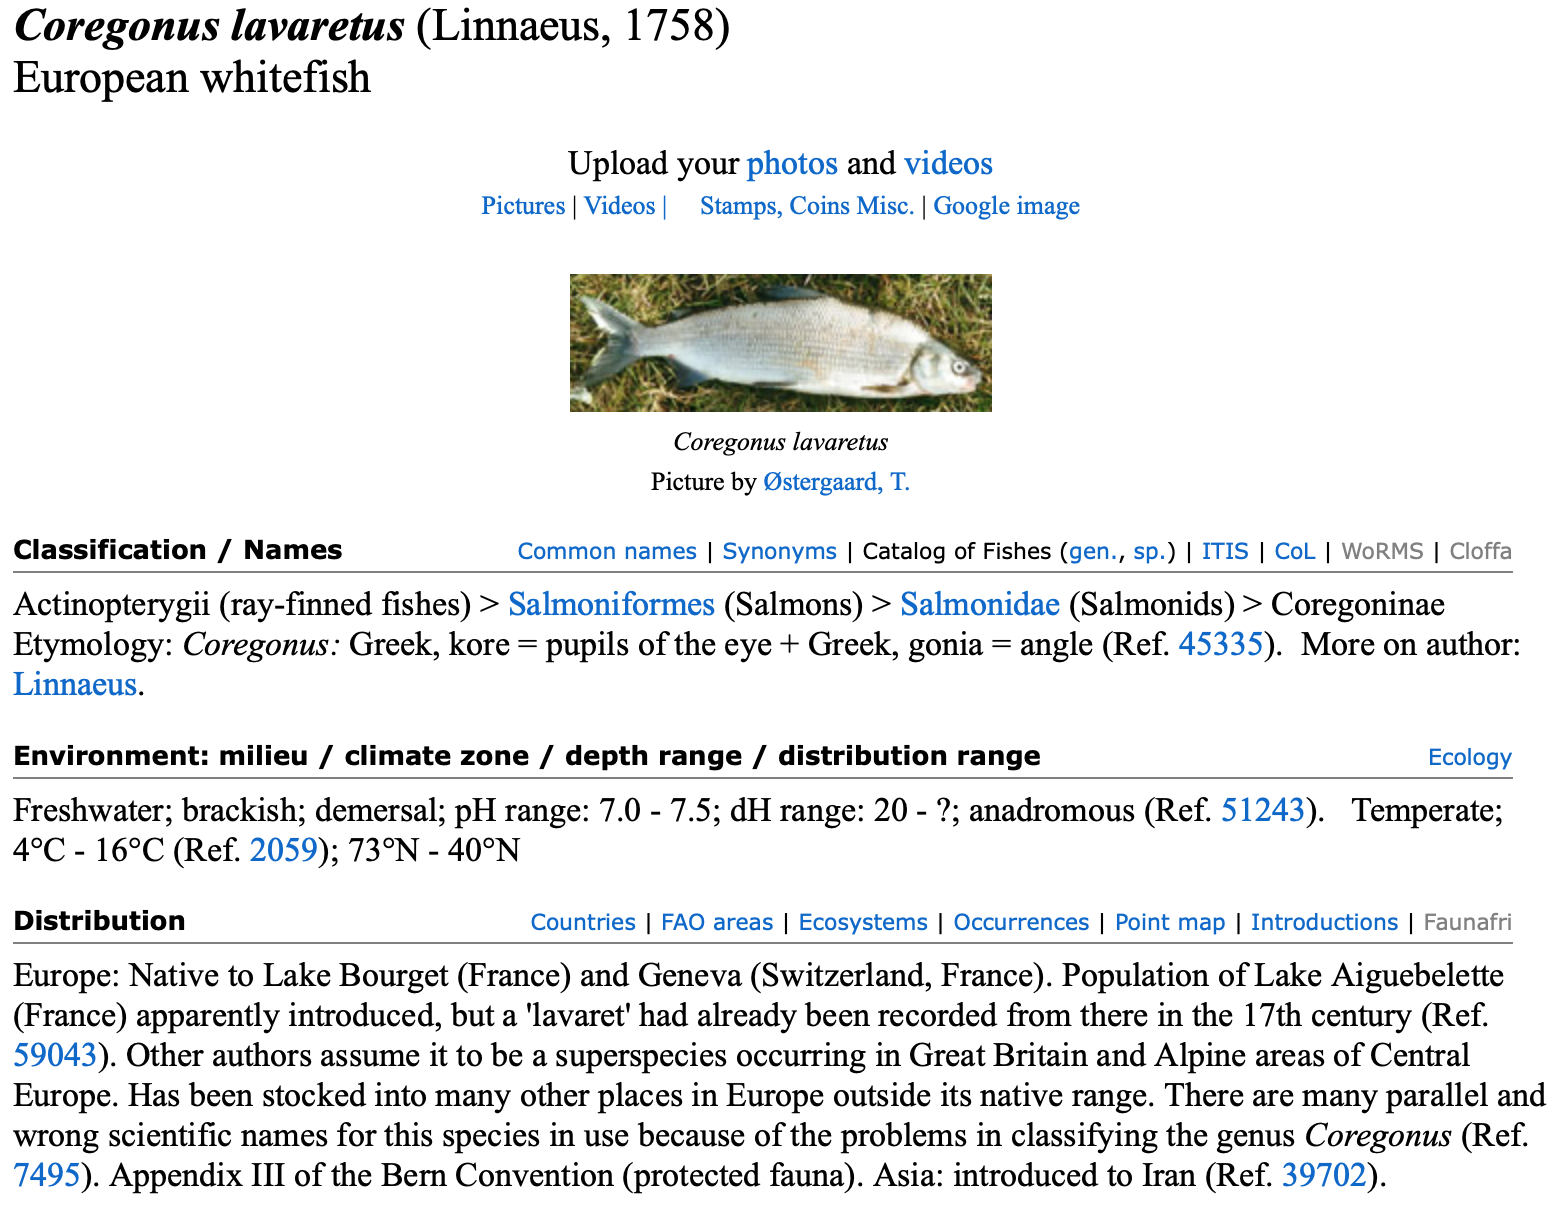
\includegraphics[width=21.67in]{./figures/screen} \caption{Screenshot of the FishBase webpage for the species *Coregonus lavaretus*, a member of the family Salmonidae. As can be read in the distribution paragraph, it is widespread in freshwater systems from central and northwest Europe to Siberia.}\label{fig:screen}
\end{figure}

As shown in Figure \ref{fig:screen}, the website contains lots of information for all the different species and this information is stored in various different data types. A few examples of these data types are:

\begin{itemize}
\tightlist
\item
  Numbers in different formats and units (temperature ranges, latitudinal distribution)
\item
  Text blocks (description of the distribution)
\item
  Tables (fecundity, larvae information)
\item
  Pictures and videos (of the species, embedded into HTML code)
\end{itemize}

For a better understanding of the following R code, you are strongly encouraged to have a look at the \href{https://fishbase.de}{FishBase} website in your browser. In the next sections you will learn how to deal with these different complex data types. A careful approach is required when extracting and downloading such information. Understanding the structure of the website is an important first step and it will save you coding time. So, always identify the relevant information you want to extract first and then write a suitable extraction code which fits the needs of your machine learning algorithm.
***
\#\#\# Accessing FishBase

We are now ready to extract data from the \emph{Coregonus lavaretus} website on \href{https://fishbase.de}{FishBase}. For this we first create a string object which holds the name of the fish profile we want to access. Using a variable to do this, adds flexibility in functions as will be shown below. If we want to get data about other species we can simply assign a new value to the object \texttt{x}with the desired species name.

\begin{Shaded}
\begin{Highlighting}[]
\NormalTok{x <-}\StringTok{ "Coregonus-lavaretus"}
\NormalTok{x}
\end{Highlighting}
\end{Shaded}

\begin{verbatim}
## [1] "Coregonus-lavaretus"
\end{verbatim}

Next, we use the function \texttt{paste()} to create an object holding the URL to the fish profile. Attaching strings like this is called concatenate and will be used quite often in later tutorials, so remember this wording. To create the URL we do not have to add any separation between the arguments, so we use \texttt{sep\ =\ ""}. Using the flexibility of using \texttt{x} allows us here to add any species name directly into \texttt{paste()} instead of deleting and adding another Latin name every time.

\begin{Shaded}
\begin{Highlighting}[]
\NormalTok{url <-}\StringTok{ }\KeywordTok{paste}\NormalTok{(}\StringTok{"http://www.fishbase.de/summary/"}\NormalTok{, x ,}\StringTok{".html"}\NormalTok{,}\DataTypeTok{sep=}\StringTok{""}\NormalTok{)}
\NormalTok{url}
\end{Highlighting}
\end{Shaded}

\begin{verbatim}
## [1] "http://www.fishbase.de/summary/Coregonus-lavaretus.html"
\end{verbatim}

For \texttt{url} we could also directly use \emph{\url{http://www.fishbase.de/summary/Coregonus-lavaretus}} but then we would loose flexibility if we want to look for information about other species.

\begin{center}\rule{0.5\linewidth}{0.5pt}\end{center}

\textbf{Checkpoint}
Try to do the same for the URL of other species by changing the code above.

\textbf{Solution}

\begin{Shaded}
\begin{Highlighting}[]
\CommentTok{# Change the object x_end to desired species name}
\NormalTok{x_ex<-}\StringTok{ "Salvelinus alpinus"}

\CommentTok{# Concatenate the URK}
\NormalTok{url_ex <-}\StringTok{ }\KeywordTok{paste}\NormalTok{(}\StringTok{"http://www.fishbase.de/summary/"}\NormalTok{,x_ex,}\StringTok{".html"}\NormalTok{,}\DataTypeTok{sep=}\StringTok{""}\NormalTok{)}
\end{Highlighting}
\end{Shaded}

\begin{center}\rule{0.5\linewidth}{0.5pt}\end{center}

To access the URL and its HTML documents, we will use various functions from the \texttt{XML} package. First, we want to get the URL content using \texttt{getURLContent()} which takes a URL as input argument. Then, we use \texttt{htmlParse()} to read the HTML document from the URL content into an R object. To get help on functions we can always use \texttt{help("htmlParse")}.

\begin{Shaded}
\begin{Highlighting}[]
\NormalTok{fishbase <-}\StringTok{ }\NormalTok{url }\OperatorTok\StringTok{ }\KeywordTok{getURLContent}\NormalTok{(}\DataTypeTok{followlocation =} \OtherTok{TRUE}\NormalTok{) }\OperatorTok\StringTok{ }\KeywordTok{htmlParse}\NormalTok{() }
\end{Highlighting}
\end{Shaded}

The HTML document saved in \texttt{fishbase} is quite long to show it entirely but a snapshot is displayed in Figure \ref{fig:fishbase}.

\begin{figure}
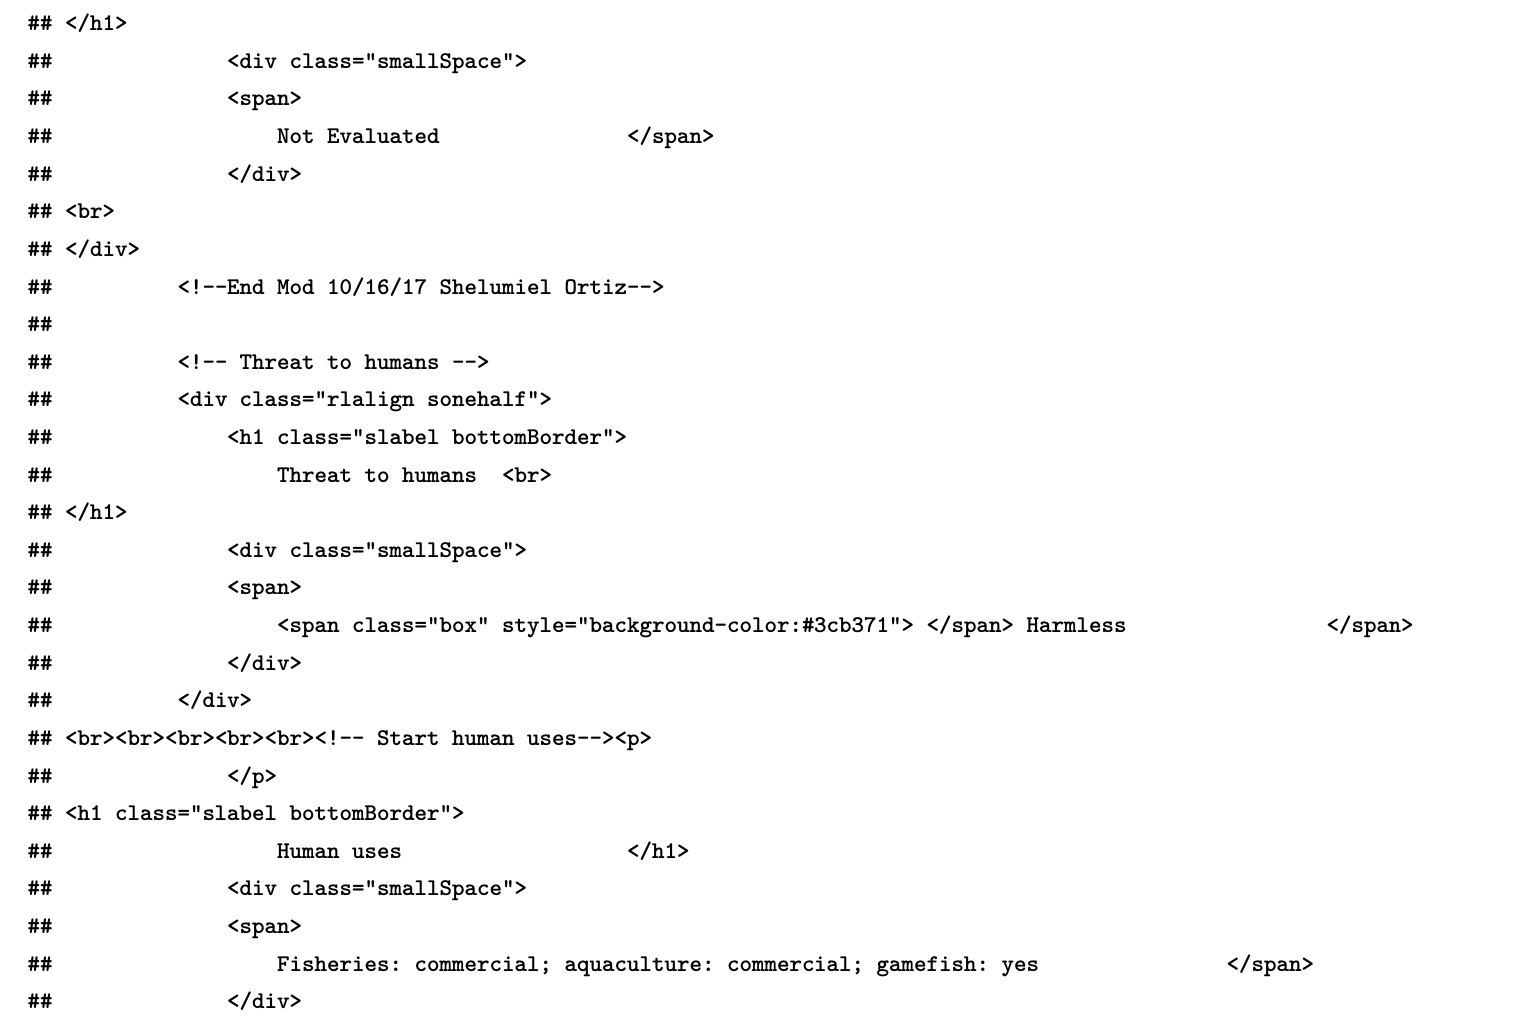
\includegraphics[width=21.14in]{./figures/fishbase} \caption{Extract from the HTML document saved in the variable `fishbase`.}\label{fig:fishbase}
\end{figure}

Somewhere in this gigantic object we can find the relevant information we are looking for. For example, Figure \ref{fig:maxle} below shows the extract where the maximal lenght of the fish is documented. Check out the online profile to double check whether the value is correct.

\begin{figure}

\includegraphics[width=18.75in]{./figures/fishbase_maxle} \caption{Extract of `fishbase` documenting maximal length of *Coregonus lavaretus*.}\label{fig:maxle}
\end{figure}

Highlighted in red are the opening and closing tags of the element where the information on the maximal length is stored. Knowing these tags, we can identify where our information is stored and how to extract it. In this example, we need to target either the \texttt{span} or \texttt{\textbackslash{}div} tags. In order to extract the information inside these two tags, we use the function \texttt{getNodeSet()}. This function finds XML nodes that match a particular criterion. \texttt{span} is used for a small chunk of HTML inside a line whereas \texttt{div} is used to group larger chunks of code.

\begin{Shaded}
\begin{Highlighting}[]
\NormalTok{fishbase_div <-}\StringTok{ }\NormalTok{fishbase }\OperatorTok\StringTok{ }\KeywordTok{getNodeSet}\NormalTok{(}\StringTok{"//div "}\NormalTok{) }
\NormalTok{fishbase_span <-}\StringTok{ }\NormalTok{fishbase }\OperatorTok\StringTok{ }\KeywordTok{getNodeSet}\NormalTok{(}\StringTok{"//span "}\NormalTok{) }
\end{Highlighting}
\end{Shaded}

In the next two Figures \ref{fig:before} and \ref{fig:after} we can see the differences of what is stored in variable \texttt{fishbase} and \texttt{fishbase\_div}. The difference to \texttt{fishbase\_span} is similar. We see that instead of having this one long unstructured extract in Figure \ref{fig:before}, we have now a list of objects that we easily access. In Figure \ref{fig:after}, the list can be identified by the \texttt{{[}{[}22{]}{]}} in the top left corner which marks the position of the object within the list. In short, \texttt{getNodeSet()} identifies all the sections for a given tag (i.e., nodes), separates them and gathers them in a list.

\begin{figure}
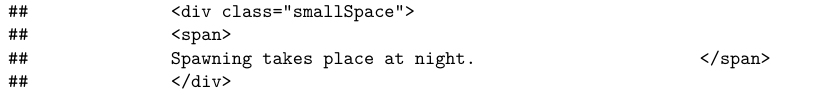
\includegraphics[width=11.47in]{./figures/before} \caption{`fishbase` before the command `getNodeSet()`}\label{fig:before}
\end{figure}

\begin{figure}
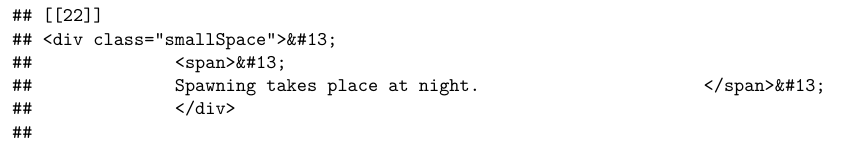
\includegraphics[width=12in]{./figures/after} \caption{`fishbase` after the command `getNodeSet()`}\label{fig:after}
\end{figure}

\begin{center}\rule{0.5\linewidth}{0.5pt}\end{center}

\hypertarget{scraping-numbers}{%
\subsection{Scraping Numbers}\label{scraping-numbers}}

Next, we now want to extract the maximal body length of \emph{Coregonus lavaretus} out of the list of nodes we created in the previous section. For this, we will use the function \texttt{xmlValue()} which allows us to access the text in the nodes by converting them into strings. To proceed further, we briefly have a look at regular expressions.

A \emph{regular expression} is basically a sequence of characters (think of a certain word or a number) that can be searched for in a string (which is nothing else but a sequence of characters). The \texttt{regexec()} (for \textbf{reg}ular \textbf{ex}pression) function allows us to search for a pattern within a string. The output of \texttt{regexec()} gives you different information. For now it enough to know that it returns a list where the first object holds the position of the pattern in the string or simply a \texttt{-1} if the pattern is not found. In our case, we are going to look for the pattern ``Max length'' because after this pattern, the value we are looking for is saved (see Figure \ref{fig:length}).

\begin{figure}
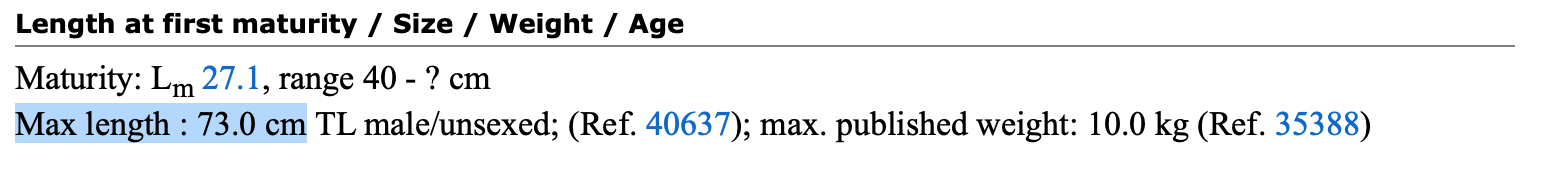
\includegraphics[width=21.72in]{./figures/length} \caption{In blue highlighted is the regular expression on the FishBase website which we are looking for.}\label{fig:length}
\end{figure}

The code to identify the position where the regular expression \emph{Max Length} is located is rather complex, so here is a step-by-step breakdown. You can run each part of the pipe below one-by-one to better understand what is happening.

\begin{Shaded}
\begin{Highlighting}[]
\NormalTok{pos <-}\StringTok{ }\NormalTok{fishbase_span }\OperatorTok\StringTok{ }\KeywordTok{lapply}\NormalTok{(xmlValue) }\OperatorTok\StringTok{  }\CommentTok{# 1. Convert all list objects in fishbase_span into strings}
\StringTok{  }\KeywordTok{regexec}\NormalTok{(}\DataTypeTok{pattern =}\StringTok{" Max length"}\NormalTok{) }\OperatorTok\StringTok{          }\CommentTok{# 2. Search strings for pattern }
\StringTok{  }\KeywordTok{which.max}\NormalTok{()                                  }\CommentTok{# 3. Return position in list where highest number is found}
                                               \CommentTok{# (just one way to identify the node with relevant information)}
\NormalTok{pos}
\end{Highlighting}
\end{Shaded}

\begin{verbatim}
## [1] 42
\end{verbatim}

Now we know that our regular expression \emph{Max length} can be found in node number 42. To get access to the text in this node we simply access \texttt{fishbase\_span} via the list notation \texttt{{[}{[}\ {]}{]}} and turn the object into a string and save it as \texttt{fish\_length}. As you can see in the output, the information on max length has been found correctly.

\begin{Shaded}
\begin{Highlighting}[]
\NormalTok{fish_length <-}\StringTok{ }\NormalTok{fishbase_span[[pos]] }\OperatorTok\StringTok{ }\KeywordTok{xmlValue}\NormalTok{()}
\NormalTok{fish_length}
\end{Highlighting}
\end{Shaded}

\begin{verbatim}
## [1] "\r\n\t\t\t\t\tMaturity: Lm27.1, range 40 - ? cm Max length : 73.0 cm TL male/unsexed; (Ref. 40637); max. published weight: 10.0 kg (Ref. 35388)\t\t\t\t"
\end{verbatim}

We now use the function \texttt{substr()}, which you already encountered in previous chapters. It allows to extract a section of a string that lies between two characters. Think of this as extracting a number interval in a series of numbers. Unfortuntaly, identifying this start and end has to be done somewhat by hand. In Figure \ref{fig:length} you can see that, starting from the \emph{`M'} in \emph{Max Length}, there are 13 characters until the value begins with a \emph{7} and 16 characters until it ends with a \emph{0}. Keep in mind that every blank space is also counted as character. Knowing this, we can first use \texttt{regexec()} to get the character position where \emph{Max Length} starts and just add 13, respectively 16 to the value.

Two things to note here: (i) Keep in mind that every blank space is also counted. (ii) Note that the output of \texttt{regexec()} is a list where the first object is the character position where the pattern begins in the string. Thus, we need to access this position number by using \texttt{{[}{[}1{]}{]}{[}1{]}}. Another way instead of using \texttt{regexec()} is just by typing in some numbers into \texttt{substr()} and find the relevant characters by trial and error.

\begin{Shaded}
\begin{Highlighting}[]
\NormalTok{start_M <-}\StringTok{ }\NormalTok{fish_length }\OperatorTok\StringTok{  }\KeywordTok{regexec}\NormalTok{(}\DataTypeTok{pattern=} \StringTok{"Max length"}\NormalTok{)}
\NormalTok{max_length <-}\StringTok{ }\NormalTok{fish_length }\OperatorTok\StringTok{ }\KeywordTok{substr}\NormalTok{(start_M[[}\DecValTok{1}\NormalTok{]][}\DecValTok{1}\NormalTok{] }\OperatorTok{+}\StringTok{ }\DecValTok{13}\NormalTok{,}
\NormalTok{                                     start_M[[}\DecValTok{1}\NormalTok{]][}\DecValTok{1}\NormalTok{] }\OperatorTok{+}\StringTok{ }\DecValTok{16}\NormalTok{)}
\NormalTok{max_length}
\end{Highlighting}
\end{Shaded}

\begin{verbatim}
## [1] "73.0"
\end{verbatim}

At last, we have to convert the value of the maximal length (which is a string of characters) into a number using the function \texttt{as.double()}. This converts the value into a machine readable format which makes things easier later. We see from the output below that we correctly exctracted a maximal length of \emph{Coregonus lavaretus} of 73 cm. Now, we can start thinking about looping this approach to extract the maximal length of various species and collect them in a nicely formatted data frame.

To demonstrate fexibility in data reading: This entire approach can also be used to for example to identify any numeric value that is followed by any one or enclosed by any two characters.

\begin{Shaded}
\begin{Highlighting}[]
\NormalTok{max_length <-}\StringTok{ }\KeywordTok{as.double}\NormalTok{(max_length)}
\NormalTok{max_length}
\end{Highlighting}
\end{Shaded}

\begin{verbatim}
## [1] 73
\end{verbatim}

\begin{center}\rule{0.5\linewidth}{0.5pt}\end{center}

\hypertarget{scraping-text-snippetrs}{%
\subsection{Scraping Text Snippetrs}\label{scraping-text-snippetrs}}

\hypertarget{international-union-for-conservation-of-nature}{%
\subsubsection*{International Union for Conservation of Nature}\label{international-union-for-conservation-of-nature}}
\addcontentsline{toc}{subsubsection}{International Union for Conservation of Nature}

Another interesting information on FishBase is the IUCN (International Union for Conservation of Nature) status of each species. The IUCN Red List of threatened Species has evolved to become the world's most comprehensive information source on the global extinction risk status of animal, fungus and plant species.

The IUCN Red List is a critical indicator of world's biodiversity and has been established in 1994. It contains explicit criteria and categories to classify the conservation status of individual species on the basis of their probability of extinction. After a species is evaluated by the IUCN, it is placed into one of eight categories based on its current conservation status as shown in the figure.

Far more than a list of species and their status, it is a powerful tool to inform and catalyze action for biodiversity conservation and policy change, critical to protecting the natural resources we depend on for survival. The IUCN also provides information about the range, population size, habitat and ecology, use and/or trade, threats, and conservation actions that will help inform necessary conservation decisions.

\begin{figure}
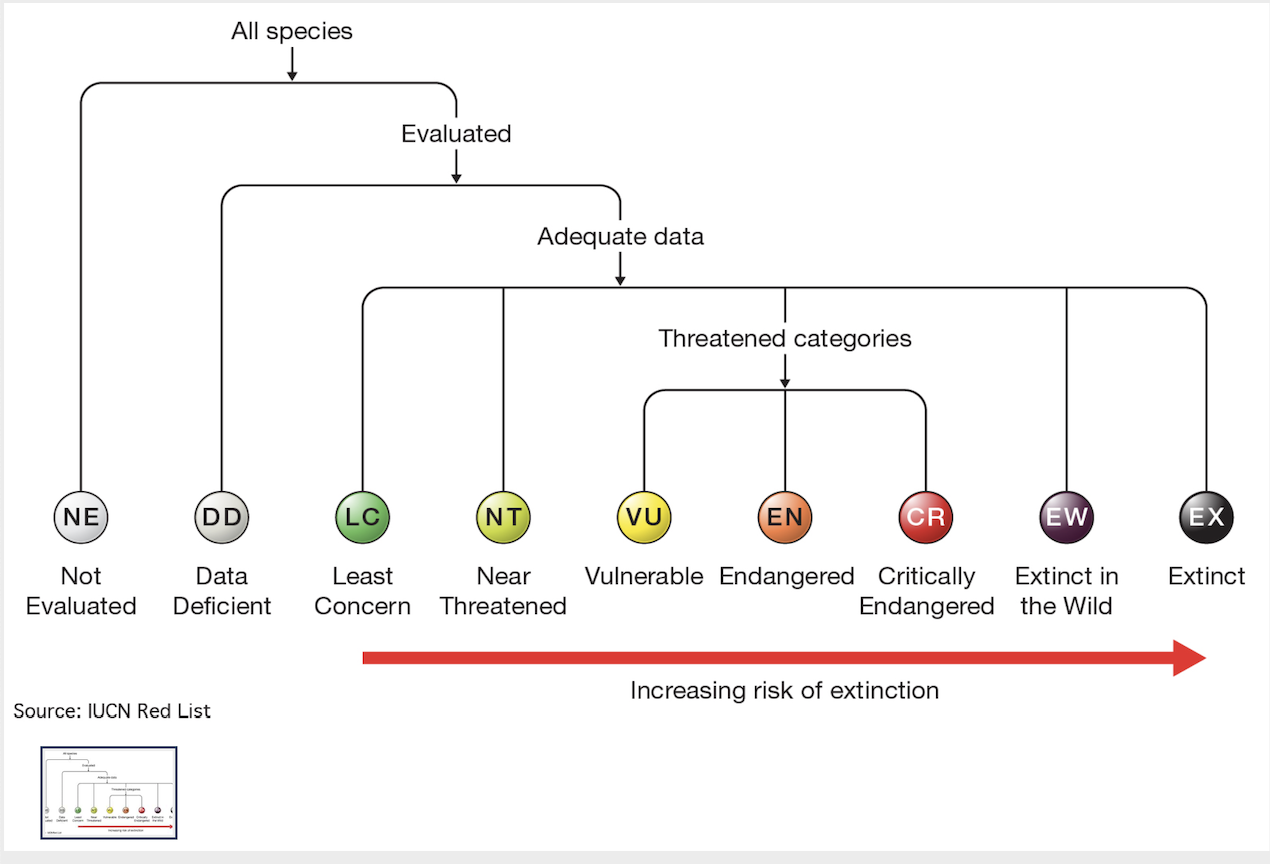
\includegraphics[width=17.64in]{./figures/iucn} \caption{Structure of IUCN categories.}\label{fig:iucn}
\end{figure}

\hypertarget{extracting-iucn-status}{%
\subsubsection*{Extracting IUCN Status}\label{extracting-iucn-status}}
\addcontentsline{toc}{subsubsection}{Extracting IUCN Status}

Now that we learned how to extract values, we can move on to extracting text snippets! In this part, we are going to get the IUCN Status of \emph{Coregonus lavaretus}. In contrary to above, we are going to use the function \texttt{which()} (not \texttt{which.max()}) to find the position of the elements we are looking for. We use \texttt{regexec()} to search for matches of our pattern within each element of a character vector. In this case, the pattern is simply \emph{IUCN}. As for the maximal length, we can look up this pattern on the website we are scraping from.

\begin{Shaded}
\begin{Highlighting}[]
\NormalTok{IUCN_pos <-}\StringTok{ }\KeywordTok{which}\NormalTok{(                 }\CommentTok{# which() gives us the numbers of nodes where pattern was found}
\NormalTok{  fishbase_div }\OperatorTok\StringTok{                 }\CommentTok{# pipe from above to find pattern put into which()}
\StringTok{    }\KeywordTok{lapply}\NormalTok{(xmlValue) }\OperatorTok\StringTok{   }
\StringTok{    }\KeywordTok{regexec}\NormalTok{(}\DataTypeTok{pattern =} \StringTok{"IUCN"}\NormalTok{)      }\CommentTok{# end of pipe}
  \OperatorTok{>}\StringTok{ }\DecValTok{0}                              \CommentTok{# check for which() to only give positive numbers for nodes}
\NormalTok{)                                  }\CommentTok{# we do this because if pattern is not found, regexec returns a -1}
   
\NormalTok{IUCN_pos                           }\CommentTok{# pattern can be found in nodes 5, 14 and 24}
\end{Highlighting}
\end{Shaded}

\begin{verbatim}
## [1]  5 14 24
\end{verbatim}

If the pattern cannot be found in \texttt{fishbase\_div}, the variable \texttt{w\_IUCN} will be empty (we use \texttt{fishbase\_div} here because the pattern was not found in \texttt{fishbase\_span}). To avoid complications later, we better do a quick check and set the variable to \texttt{NA} if it is empty and else use \texttt{xmlValue()} to get the value at the last node where the pattern was found.

\begin{Shaded}
\begin{Highlighting}[]
\ControlFlowTok{if}\NormalTok{(}\KeywordTok{length}\NormalTok{(IUCN_pos)}\OperatorTok{==}\DecValTok{0}\NormalTok{)\{              }\CommentTok{# if which() from above returned 0 (no node with >0)}
\NormalTok{  IUCN_stat =}\StringTok{ "NA"}                    \CommentTok{# set status to NA}
\NormalTok{\} }\ControlFlowTok{else}\NormalTok{ \{                              }\CommentTok{# else}
\NormalTok{  IUCN_xml <-}\StringTok{ }\NormalTok{fishbase_div[[          }\CommentTok{# access fishbase_div nodes with [[}
\NormalTok{    IUCN_pos[}\KeywordTok{length}\NormalTok{(IUCN_pos)]]] }\OperatorTok\StringTok{  }\CommentTok{# access last node where pattern was found, length(IUCN_pos) = 24}
\StringTok{    }\KeywordTok{xmlValue}\NormalTok{()                        }\CommentTok{# feed node into xmlValue() to return readable string}
\NormalTok{\}}

\NormalTok{IUCN_xml}
\end{Highlighting}
\end{Shaded}

\begin{verbatim}
## [1] "\r\n\t\t\t\t\r\n\t\t\t\t\tIUCN Red List Status   (Ref. 120744)\r\n\t\t\t\t\r\n\t\t\t\t\r\n\t\t\t\t\t  Vulnerable (VU) (D2); Date assessed: 01 January 2008\t\t\t\t\r\n\t\t\t\t"
\end{verbatim}

The \texttt{IUCN\_xml} looks a little confusing and we only need a tiny part of it, namely \emph{VU}. We can see that in this node \emph{VU} has a unique character pattern which does not appear twice: The closing bracket \texttt{)}is right after \texttt{U}, an alphabetical character. We can use this pattern to extract \emph{VU}! Here, the \texttt{str\_extract()} function from tidyverse comes in very handy. We can directly specify the pattern we are looking for and extract the substring from the original string. Note that for generalization, we need to specify \texttt{{[}{[}:alpha:{]}{]}} for any alphabetical character \texttt{+{[}){]}} for the closing bracket.

However, if we do so, we still extract the bracket as well. To get rid of it, we can simply remove it by replacing it with ``nothing'' using \texttt{str\_replace()}. Instead of specifying the closing bracket, we use \texttt{{[}:punct:{]}} which generalizes punctuations like \texttt{.\ ,\ :\ ;\ ?\ !} etc. As we see in the output below, the IUCN status \emph{VU} has been correctly extracted - nice! Plus, we don't need to convert it and can use it as string later on.

\begin{Shaded}
\begin{Highlighting}[]
\NormalTok{IUCN_sta <-}\StringTok{ }\NormalTok{IUCN_xml }\OperatorTok
\StringTok{  }\KeywordTok{str_extract}\NormalTok{(}\DataTypeTok{pattern =} \StringTok{"[:alpha:]+[)]"}\NormalTok{) }\OperatorTok
\StringTok{  }\KeywordTok{str_replace}\NormalTok{(}\DataTypeTok{pattern =} \StringTok{"[:punct:]"}\NormalTok{, }\DataTypeTok{replacement =} \StringTok{""}\NormalTok{)}

\NormalTok{IUCN_sta}
\end{Highlighting}
\end{Shaded}

\begin{verbatim}
## [1] "VU"
\end{verbatim}

\begin{center}\rule{0.5\linewidth}{0.5pt}\end{center}

\hypertarget{scraping-tables}{%
\subsection{Scraping Tables}\label{scraping-tables}}

The next step is to read a table from a website. Here, we are going to get information on the eggs of \emph{Coregonus lavaretus}. Have a look at its \href{https://www.fishbase.de/summary/Coregonus-lavaretus.html}{profile}. In section \textbf{Life cycle and mating behavior} you can see that the table for information on eggs is a link and not a table directly. Foruntatley for us, we can use the function \texttt{getHTMLLinks()} to retrieve links within an HTML document or the collection of names of external files referenced in an HTML document. In Figure \ref{fig:eggs}, an extract is shown of the list with more than 100 links found on the profile page.

We see that either we could directly access link number 100 or search for the substring \emph{FishEggInfoSummary} to look for other links. In fact, we will find two links with this substring (see Figure \ref{fig:outputlink}. For this reason, we quickly check if the links are identical of if they lead to different pages. We can do this by using the logic operator \texttt{==}. The link comparison gives \texttt{TRUE} as output meaning that both links are completely identical and it does not matter which one we use. Let us save the first one in \texttt{egg\_link}.

\begin{Shaded}
\begin{Highlighting}[]
\NormalTok{egg_link <-}\StringTok{ }\NormalTok{fishbase }\OperatorTok\StringTok{ }\KeywordTok{getHTMLLinks}\NormalTok{() }\OperatorTok
\StringTok{  }\KeywordTok{str_subset}\NormalTok{(}\DataTypeTok{pattern =} \StringTok{"FishEggInfoSummary"}\NormalTok{)}

\NormalTok{egg_link[}\DecValTok{1}\NormalTok{] }\OperatorTok{==}\StringTok{ }\NormalTok{egg_link[}\DecValTok{2}\NormalTok{]}
\end{Highlighting}
\end{Shaded}

\begin{verbatim}
## [1] TRUE
\end{verbatim}

\begin{Shaded}
\begin{Highlighting}[]
\NormalTok{egg_link <-}\StringTok{ }\NormalTok{egg_link[}\DecValTok{1}\NormalTok{]}
\end{Highlighting}
\end{Shaded}

\begin{figure}
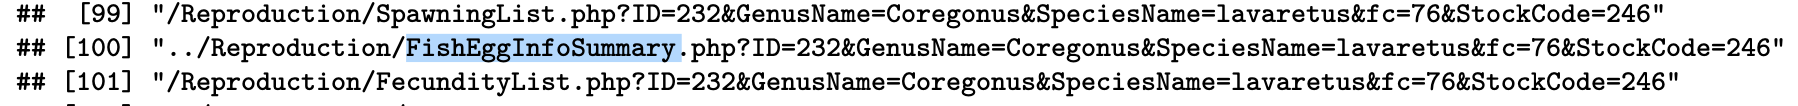
\includegraphics[width=24.97in]{./figures/eggs} \caption{Extract of the list of links found on the FishBase profile of *Coregonus lavaretus*.}\label{fig:eggs}
\end{figure}
\begin{figure}

\includegraphics[width=24.36in]{./figures/outputlink} \caption{List of links that have the substring *FishEggInfoSummary*.}\label{fig:outputlink}
\end{figure}

\begin{center}\rule{0.5\linewidth}{0.5pt}\end{center}

\textbf{Checkpoint}
Call the variable \emph{egg\_link}, you will notice the link begins with `..' (see above \ref{fig:outputlink}). Try to remove these dots so that the link begins with `/Reproduction/..'. As a hint, you can use the function \texttt{str\_replace()} as was done above. You will need this code later, so make sure that you run it.

\begin{Shaded}
\begin{Highlighting}[]
\CommentTok{# your code}
\end{Highlighting}
\end{Shaded}

\textbf{Solution}

\begin{Shaded}
\begin{Highlighting}[]
\NormalTok{egg_link <-}\StringTok{ }\NormalTok{egg_link }\OperatorTok\StringTok{ }\KeywordTok{str_replace}\NormalTok{(}\StringTok{".."}\NormalTok{, }\StringTok{""}\NormalTok{ )}
\NormalTok{egg_link}
\end{Highlighting}
\end{Shaded}

\begin{verbatim}
## [1] "/Reproduction/FishEggInfoSummary.php?ID=232&GenusName=Coregonus&SpeciesName=lavaretus&fc=76&StockCode=246"
\end{verbatim}

\begin{center}\rule{0.5\linewidth}{0.5pt}\end{center}

As you can see, this is no proper URL yet. Thus, we first need to create a working URL to access its content. Similarly to what we did previously, we do this using the function \texttt{getURLContent()}. Since we know that this link leads to a table, we can pipe the URL content into \texttt{readHTMLTable()}. The output here is a list and we have access the first object as done below.

\begin{Shaded}
\begin{Highlighting}[]
\NormalTok{egg_tab <-}\StringTok{ }\KeywordTok{paste}\NormalTok{(}\StringTok{"http://www.fishbase.de/"}\NormalTok{, egg_link, }\DataTypeTok{sep=}\StringTok{""}\NormalTok{) }\OperatorTok
\StringTok{  }\KeywordTok{getURLContent}\NormalTok{(}\DataTypeTok{followlocation=}\OtherTok{TRUE}\NormalTok{, }\DataTypeTok{.encoding=}\StringTok{"CE_UTF8"}\NormalTok{) }\OperatorTok
\StringTok{  }\KeywordTok{readHTMLTable}\NormalTok{()}

\NormalTok{egg_tab <-}\StringTok{ }\NormalTok{egg_tab[[}\DecValTok{1}\NormalTok{]] }\CommentTok{# To save the list object as a data frame}
\NormalTok{egg_tab}
\end{Highlighting}
\end{Shaded}

\begin{verbatim}
##               Main Ref.       
## 1  Place of Development       
## 2          Shape of Egg       
## 3            Attributes       
## 4         Color of Eggs       
## 5  Color of Oil Globule       
## 6 Additional Characters       
## 7    Get Information on Scirus
\end{verbatim}

Now we can extract information from this table by using the function \texttt{which()}. We want to find the position in this table, where \emph{Shape of Egg} is defined. To identify the right row, we look in the first column for the respective string and extract the value stored in the second column of this row. To automatize, we add a check to see whether any information was extracted at all from the table. If not (as it is the case here), we just set \texttt{egg\_shape} to NA.

\begin{Shaded}
\begin{Highlighting}[]
\NormalTok{egg_shape <-}\StringTok{ }\NormalTok{egg_tab[                     }\CommentTok{# Accessing rows of egg_tab (remember: df[rows, cols])}
  \KeywordTok{which}\NormalTok{(egg_tab[, }\DecValTok{1}\NormalTok{] }\OperatorTok{==}\StringTok{ "Shape of Egg"}\NormalTok{),  }\CommentTok{# Get number of row where "Shape of Egg" appears in the first column}
  \DecValTok{2}\NormalTok{]                                      }\CommentTok{# Access the second column}

\NormalTok{egg_shape}
\end{Highlighting}
\end{Shaded}

\begin{verbatim}
## [1] ""
\end{verbatim}

\begin{Shaded}
\begin{Highlighting}[]
\ControlFlowTok{if}\NormalTok{(egg_shape }\OperatorTok{==}\StringTok{ ""}\NormalTok{) \{egg_shape =}\StringTok{ "NA"}\NormalTok{\}}
\NormalTok{egg_shape}
\end{Highlighting}
\end{Shaded}

\begin{verbatim}
## [1] "NA"
\end{verbatim}

Now we can put all the information into a data frame for the entry \emph{Coregonus lavaretus} by using the function \texttt{tibble()}. Having done this entire data scraping for one species, we can start to automatize the process for multiple species and simply append the data to our data frame.

\begin{Shaded}
\begin{Highlighting}[]
\NormalTok{species_df <-}\StringTok{ }\KeywordTok{tibble}\NormalTok{(}\DataTypeTok{Species =} \StringTok{"Coregonus-lavaretus"}\NormalTok{, }\DataTypeTok{Length =}\NormalTok{ max_length, }\DataTypeTok{IUCN =}\NormalTok{ IUCN_sta, }\DataTypeTok{Egg =}\NormalTok{ egg_shape)}
\NormalTok{species_df}
\end{Highlighting}
\end{Shaded}

\begin{verbatim}
## # A tibble: 1 x 4
##   Species             Length IUCN  Egg  
##   <chr>                <dbl> <chr> <chr>
## 1 Coregonus-lavaretus     73 VU    NA
\end{verbatim}

\begin{center}\rule{0.5\linewidth}{0.5pt}\end{center}

\textbf{Checkpoint}
Try to create and add a new variable \emph{egg\_color} to the data frame and feed it with the respective information from our \texttt{egg\_table} (follow the same process used for `egg\_shape').

\begin{Shaded}
\begin{Highlighting}[]
\CommentTok{# your code }
\end{Highlighting}
\end{Shaded}

\textbf{Solution}

\begin{Shaded}
\begin{Highlighting}[]
\NormalTok{egg_color =}\StringTok{ }\NormalTok{egg_tab[}\KeywordTok{which}\NormalTok{(egg_tab[, }\DecValTok{1}\NormalTok{] }\OperatorTok{==}\StringTok{ "Color of Eggs"}\NormalTok{), }\DecValTok{2}\NormalTok{]  }\CommentTok{# extract information}
\ControlFlowTok{if}\NormalTok{(egg_color }\OperatorTok{==}\StringTok{ ""}\NormalTok{)\{egg_color =}\StringTok{ "NA"}\NormalTok{\}                           }\CommentTok{# set missing information to NA}
\NormalTok{species_df <-}\StringTok{ }\KeywordTok{tibble}\NormalTok{(species_df, }\DataTypeTok{Color =}\NormalTok{ egg_color)             }\CommentTok{# Add new variable to data frane}
\NormalTok{species_df}
\end{Highlighting}
\end{Shaded}

\begin{verbatim}
## # A tibble: 1 x 5
##   Species             Length IUCN  Egg   Color
##   <chr>                <dbl> <chr> <chr> <chr>
## 1 Coregonus-lavaretus     73 VU    NA    NA
\end{verbatim}

\begin{center}\rule{0.5\linewidth}{0.5pt}\end{center}

\hypertarget{the-fishbase-package}{%
\subsection{The Fishbase Package}\label{the-fishbase-package}}

\hypertarget{using-an-api}{%
\subsubsection*{Using an API}\label{using-an-api}}
\addcontentsline{toc}{subsubsection}{Using an API}

As we saw in the previous sections, web scraping can be tedious. In this subsection, we want to get data using an API which is a much easier way. We use the R package \texttt{rfishbase} to get data from \url{https://www.fishbase.de}. This package makes it very easy to look up for information on the most well-known fish species. It simplifies the data extraction process but also has some limits as we will see below. You ca have a look at the functions built into \texttt{rfishbase} by typing \texttt{help(package\ =\ "rfishbase")} into your RStudio console or have a look at the \href{https://www.rdocumentation.org/packages/rfishbase/versions/3.0.4}{RDocumentation}. Most functions have straight forward names and have a sring as input which holds the Latin name of the wanted fish species.

Let us get some information on \emph{Coregonus lavaretus} with this new package! We see that the super short code \texttt{species("Coregonus\ lavaretus")}provides us with 101 variables with entries for our fish species - think about the hand-written web scraping code this would require! To directly asses the maximal length of the species, we can directly use the \texttt{\$} notation. As you might recall, this is the same length as we got above.

\begin{Shaded}
\begin{Highlighting}[]
\NormalTok{CL <-}\StringTok{ }\KeywordTok{species}\NormalTok{(}\StringTok{"Coregonus lavaretus"}\NormalTok{)}
\NormalTok{CL}\OperatorTok{$}\NormalTok{Length}
\end{Highlighting}
\end{Shaded}

\begin{verbatim}
## [1] 73
\end{verbatim}

In the next step we are interested to get information about the diet of \emph{Coregonus lavaretus} by using the function \texttt{diet\_items()}. It allows us to access the table on the food items of the chosen species. To extract information on food, we can save the diet items in a table and use the tidyverse notation plus the respective variables \emph{FoodI}, \emph{FoodII}:

\begin{Shaded}
\begin{Highlighting}[]
\NormalTok{food <-}\StringTok{ }\KeywordTok{diet_items}\NormalTok{(}\StringTok{"Coregonus lavaretus"}\NormalTok{) }\OperatorTok\StringTok{ }\NormalTok{as_tibble}
\NormalTok{food }\OperatorTok\StringTok{ }\NormalTok{dplyr}\OperatorTok{::}\KeywordTok{select}\NormalTok{(FoodI, FoodII) }\OperatorTok\StringTok{ }\KeywordTok{head}\NormalTok{() }\CommentTok{# We're using dplyr:: here to avoid package conflicts}
\end{Highlighting}
\end{Shaded}

\begin{verbatim}
## # A tibble: 6 x 2
##   FoodI      FoodII       
##   <chr>      <chr>        
## 1 zoobenthos mollusks     
## 2 nekton     finfish      
## 3 zoobenthos benth. crust.
## 4 zoobenthos worms        
## 5 zoobenthos benth. crust.
## 6 zoobenthos benth. crust.
\end{verbatim}

\begin{center}\rule{0.5\linewidth}{0.5pt}\end{center}

\textbf{Checkpoint}
Now your next task is to get information on predators (hint: the function is exactly named like that).

\begin{Shaded}
\begin{Highlighting}[]
\CommentTok{# your code}
\end{Highlighting}
\end{Shaded}

\textbf{Solution}

\begin{Shaded}
\begin{Highlighting}[]
\CommentTok{# use function 'predators()' for Coregonus lavaretus}
\NormalTok{pre <-}\StringTok{ }\KeywordTok{predators}\NormalTok{(}\StringTok{"Coregonus lavaretus"}\NormalTok{)}
\NormalTok{pre }\OperatorTok\StringTok{ }\NormalTok{dplyr}\OperatorTok{::}\KeywordTok{select}\NormalTok{(PredatorName) }\OperatorTok\StringTok{ }\KeywordTok{head}\NormalTok{()}
\end{Highlighting}
\end{Shaded}

\begin{verbatim}
## # A tibble: 6 x 1
##   PredatorName       
##   <chr>              
## 1 Coregonus peled    
## 2 Esox lucius        
## 3 Salmo trutta trutta
## 4 Sander lucioperca  
## 5 Phryganea sp.      
## 6 Coregonus lavaretus
\end{verbatim}

\begin{center}\rule{0.5\linewidth}{0.5pt}\end{center}

\hypertarget{limits-of-apis}{%
\subsubsection*{Limits of APIs}\label{limits-of-apis}}
\addcontentsline{toc}{subsubsection}{Limits of APIs}

One of the major limitations of an API is that we can only use already implemented functions. For example, in our case, we cannot get the IUCN Status of a given species because it is not built into \texttt{rfishbase}. In order to obtain the IUCN Status we must use another API, namely the package \texttt{rredlist}. Unfortunately, to have access to the \emph{rredlist} API we need an authentication key which we only get for a small fee. As it is with other things in life, either you try to put in the work yourself or you can pay someone to do so (except for the amazing open source community).

\hypertarget{summary}{%
\subsection{Summary}\label{summary}}

\begin{itemize}
\tightlist
\item
  In this third section we learned how to extract data from a website.
\item
  We saw that this can be done either with web scraping or using APIs.
\item
  We saw that web scraping can be tedious, but we learned about some limitations of APIs.
\end{itemize}

\begin{center}\rule{0.5\linewidth}{0.5pt}\end{center}

\hypertarget{case-study-species-richness-and-red-list-species-proportions}{%
\section{Case Study: Species Richness and Red List species proportions}\label{case-study-species-richness-and-red-list-species-proportions}}

\emph{Please note that the code below is written in base R and not tidyverse which makes the codes a bit more difficult to read. But do not worry about this and simply just enjoy the beauty of what R is capable of.}

Next, we look at another case study on species richness and red list species proportions. To proceed with the case study we need to prepare our dataset. First, we need to get a list of species for the dataset. In this subsection we will see how to get all the species in a given family.

\begin{center}\rule{0.5\linewidth}{0.5pt}\end{center}

\hypertarget{creating-list-of-species}{%
\subsection{Creating List of Species}\label{creating-list-of-species}}

In this section, we want to get all the species of the family of \emph{Salmonidae}. As we did above, for flexibility we will create an object \emph{x} with the name of the family and use \texttt{paste()} to get the link.
We then use \texttt{getURLContent()} to get the content of the link \texttt{url} and save it in \texttt{con\_sal}.

\begin{Shaded}
\begin{Highlighting}[]
\NormalTok{x <-}\StringTok{ "Salmonidae"}
\NormalTok{url <-}\StringTok{ }\KeywordTok{paste}\NormalTok{(}\StringTok{"http://www.fishbase.de/Nomenclature/FamilySearchList.php?Family="}\NormalTok{, x, }\DataTypeTok{sep=}\StringTok{""}\NormalTok{) }
\NormalTok{con_sal <-}\StringTok{ }\KeywordTok{getURLContent}\NormalTok{(url, }\DataTypeTok{followlocation =} \OtherTok{TRUE}\NormalTok{) }
\end{Highlighting}
\end{Shaded}

Next we create a dataframe using \texttt{data.frame()} and get a list of variables. We will extract the variables with the same number of rows and unique row names. The function \texttt{readHTMLTable()} (from earlier) helps to extract data from HTML tables in an HTML document. Then we can extract the species from the given family with \texttt{as.character()}. We use \texttt{z{[},1{]}} to get the first column which is the column with the scientific names of species. Now we can print the first element of the column with the scientific names.

\begin{Shaded}
\begin{Highlighting}[]
\NormalTok{df <-}\StringTok{ }\KeywordTok{data.frame}\NormalTok{(}\KeywordTok{readHTMLTable}\NormalTok{(con_sal))}
\NormalTok{sp_per_family <-}\StringTok{ }\KeywordTok{as.character}\NormalTok{(df[,}\DecValTok{1}\NormalTok{])}
\NormalTok{sp_per_family[}\DecValTok{1}\NormalTok{]}
\end{Highlighting}
\end{Shaded}

\begin{verbatim}
## [1] "Brachymystax lenok"
\end{verbatim}

Using \texttt{str\_replace()} function we can substitute the empty space between the Genus and the Species with a \texttt{"-"}. Finally we can print the first element of \emph{sp\_per\_family} again.

\begin{Shaded}
\begin{Highlighting}[]
\NormalTok{sp_per_family <-}\StringTok{ }\KeywordTok{str_replace}\NormalTok{(sp_per_family, }\StringTok{" "}\NormalTok{, }\StringTok{"-"}\NormalTok{)}
\NormalTok{sp_per_family[}\DecValTok{1}\NormalTok{]}
\end{Highlighting}
\end{Shaded}

\begin{verbatim}
## [1] "Brachymystax-lenok"
\end{verbatim}

\begin{center}\rule{0.5\linewidth}{0.5pt}\end{center}

\hypertarget{extracting-iucn-status-for-all-species}{%
\subsection{Extracting IUCN Status for all species}\label{extracting-iucn-status-for-all-species}}

In this section, we are going to get the IUCN Status for a given List of species using a `for loop'. We will extract the IUCN Status of all the species from the Netherlands.
First, we are going to upload the dataset containing the list of the species and some other data that is going to be useful for the next sections. We will do that by using the function \texttt{read\_csv()}. This data is taken from this \href{https://www.nature.com/articles/sdata2017141}{nature article} by cropping it to Western Europe. As we only need data related to Netherlands, we will use the function \texttt{grep()} and pass \emph{Netherlands} as an argument.

\begin{Shaded}
\begin{Highlighting}[]
\NormalTok{dataset <-}\StringTok{ }\KeywordTok{read_csv}\NormalTok{(}\StringTok{"./data/dataset2.csv"}\NormalTok{)}
\NormalTok{subset <-}\StringTok{ }\NormalTok{dataset[}\KeywordTok{grep}\NormalTok{(}\StringTok{"Netherlands"}\NormalTok{, dataset}\OperatorTok{$}\NormalTok{Country),]}
\end{Highlighting}
\end{Shaded}

Let us first briefly discuss how to construct a `for loop', since it's been a while since you used it in previous chapters. To get the IUCN Status of a list of species we always change the value of \emph{x} (the species) and run the code, but if we have to do that for many species it will be very long and tedious. In this case `for loops' come in handy. In a `for loop' the variable \emph{x} runs over the vector (here each species) and returns the IUCN Status. Before getting the IUCN status we will go over an easy example, such as printing the integers from 1 to 10 using a `for loop'. In this case, we iterate over the vector 1:10.

\begin{Shaded}
\begin{Highlighting}[]
\ControlFlowTok{for}\NormalTok{(j }\ControlFlowTok{in} \DecValTok{1}\OperatorTok{:}\DecValTok{10}\NormalTok{) \{}
\KeywordTok{print}\NormalTok{(j) }\CommentTok{# this prints the value of j for that given loop}
\NormalTok{\}}
\end{Highlighting}
\end{Shaded}

\begin{verbatim}
## [1] 1
## [1] 2
## [1] 3
## [1] 4
## [1] 5
## [1] 6
## [1] 7
## [1] 8
## [1] 9
## [1] 10
\end{verbatim}

Now we can make a `for loop' in order to get the IUCN status of all the species in the above subset (Netherlands) of the initial dataset. We are going to iterate over the column of the dataset with the valid FishBase species names. The code lines inside the loop are exactly a copy-paste of what we had for the \emph{Coregonus lavaretus}, but in this case, we have to look for other species. In the last line of the code below, we created a new column in the data frame \emph{subset} in order to save the IUCN Status. The `i' in \texttt{subset\$IUCN{[}i{]}} is used to save the IUCN status of the species we are iterating over in the `for loop'. It will save the results of the species one by one.

\begin{Shaded}
\begin{Highlighting}[]
\NormalTok{i <-}\StringTok{ }\DecValTok{0}
\ControlFlowTok{for}\NormalTok{(x }\ControlFlowTok{in}\NormalTok{ subset}\OperatorTok{$}\NormalTok{X6.Fishbase.Valid.Species.Name) \{}
\NormalTok{  i <-}\StringTok{ }\NormalTok{i }\OperatorTok{+}\StringTok{ }\DecValTok{1}
  
\NormalTok{  url <-}\StringTok{ }\KeywordTok{paste}\NormalTok{(}\StringTok{"http://www.fishbase.de/summary/"}\NormalTok{,x,}\StringTok{".html"}\NormalTok{,}\DataTypeTok{sep=}\StringTok{""}\NormalTok{)       }\CommentTok{# we call the url}
\NormalTok{  fish_species <-}\StringTok{ }\KeywordTok{htmlParse}\NormalTok{(}\KeywordTok{getURLContent}\NormalTok{(url, }\DataTypeTok{followlocation=}\OtherTok{TRUE}\NormalTok{))     }\CommentTok{# get the content}
\NormalTok{  fish_species_div <-}\KeywordTok{getNodeSet}\NormalTok{(fish_species, }\StringTok{"//div "}\NormalTok{)                  }\CommentTok{# get the nodes with species}
\NormalTok{  w_IUCN  <-}\StringTok{ }\KeywordTok{which}\NormalTok{(}\KeywordTok{sapply}\NormalTok{(}\KeywordTok{lapply}\NormalTok{(fish_species_div,xmlValue),}\ControlFlowTok{function}\NormalTok{(x)  }\CommentTok{# look for the IUCN pattern }
\NormalTok{    \{}\KeywordTok{regexec}\NormalTok{(}\DataTypeTok{pattern=}\StringTok{"IUCN"}\NormalTok{, x)[[}\DecValTok{1}\NormalTok{]][}\DecValTok{1}\NormalTok{]\})}\OperatorTok{>}\DecValTok{0}\NormalTok{)}
  
  \ControlFlowTok{if}\NormalTok{(}\KeywordTok{length}\NormalTok{(w_IUCN)}\OperatorTok{==}\DecValTok{0}\NormalTok{)\{                                                 }\CommentTok{# NA if no IUCN status}
\NormalTok{    IUCN_status=}\StringTok{"NA"}
\NormalTok{\} }\ControlFlowTok{else}\NormalTok{ \{                                                                 }\CommentTok{# else access information}
\NormalTok{    d1_IUCN  <-}\StringTok{ }\KeywordTok{xmlValue}\NormalTok{(fish_species_div[[w_IUCN[}\KeywordTok{length}\NormalTok{(w_IUCN)]]])}
\NormalTok{    IUCN <-}\StringTok{ }\KeywordTok{unlist}\NormalTok{(}\KeywordTok{regmatches}\NormalTok{(d1_IUCN,}\KeywordTok{gregexpr}\NormalTok{(}\DataTypeTok{pattern=} \StringTok{"[[:alpha:]]+)"}\NormalTok{,     }
\NormalTok{    d1_IUCN)))}
\NormalTok{    IUCN_status <-}\StringTok{ }\KeywordTok{sub}\NormalTok{(}\DataTypeTok{pattern=}\StringTok{"[[:punct:]]"}\NormalTok{,}\DataTypeTok{replacement=}\StringTok{""}\NormalTok{,IUCN[}\DecValTok{1}\NormalTok{] ) }
\NormalTok{\}}
  
\KeywordTok{print}\NormalTok{(IUCN_status)}
\NormalTok{subset}\OperatorTok{$}\NormalTok{IUCN[i] <-}\StringTok{ }\NormalTok{IUCN_status }\CommentTok{# make a new column in 'subset' containing the IUCN status}
\NormalTok{\}}
\end{Highlighting}
\end{Shaded}

\begin{verbatim}
## [1] "LC"
## [1] "LC"
## [1] "LC"
## [1] "LC"
## [1] "LC"
## [1] "LC"
## [1] "VU"
## [1] NA
## [1] NA
\end{verbatim}

We can see which IUCN statuses are present in Netherlands by using the \texttt{unique()} function. There are LC for least concern, VU for vulnerable and of course NA for unknown values.

\begin{Shaded}
\begin{Highlighting}[]
\KeywordTok{unique}\NormalTok{(subset}\OperatorTok{$}\NormalTok{IUCN)}
\end{Highlighting}
\end{Shaded}

\begin{verbatim}
## [1] "LC" "VU" NA
\end{verbatim}

\begin{center}\rule{0.5\linewidth}{0.5pt}\end{center}

\hypertarget{proportion-of-species-in-netherlands}{%
\subsection{Proportion of species in Netherlands}\label{proportion-of-species-in-netherlands}}

We will now plot the proportion of species in each category for the Netherlands. So let us calculate the number of species in each category (from above we just have 2 outputs,* \emph{LC} \& \emph{NT}). In general in other countries, we also have other IUCN Status, for example, VU. In this section, we will focus only on the two listed statuses. Using the function \texttt{length()} we can obtain the number of species in each category.

\begin{Shaded}
\begin{Highlighting}[]
\NormalTok{number_lc <-}\StringTok{ }\KeywordTok{length}\NormalTok{(}\KeywordTok{which}\NormalTok{(subset}\OperatorTok{$}\NormalTok{IUCN }\OperatorTok{==}\StringTok{ "LC"}\NormalTok{))}
\NormalTok{number_vu <-}\StringTok{ }\KeywordTok{length}\NormalTok{(}\KeywordTok{which}\NormalTok{(subset}\OperatorTok{$}\NormalTok{IUCN }\OperatorTok{==}\StringTok{ "VU"}\NormalTok{))}
\NormalTok{number_na <-}\StringTok{ }\KeywordTok{length}\NormalTok{(}\KeywordTok{which}\NormalTok{(}\KeywordTok{is.na}\NormalTok{(subset}\OperatorTok{$}\NormalTok{IUCN)))}

\CommentTok{# print the values for NT, VU and NA}
\KeywordTok{paste0}\NormalTok{(}\StringTok{"LC:"}\NormalTok{, }\StringTok{" "}\NormalTok{, number_lc)}
\end{Highlighting}
\end{Shaded}

\begin{verbatim}
## [1] "LC: 6"
\end{verbatim}

\begin{Shaded}
\begin{Highlighting}[]
\KeywordTok{paste0}\NormalTok{(}\StringTok{"VU:"}\NormalTok{, }\StringTok{" "}\NormalTok{, number_vu)}
\end{Highlighting}
\end{Shaded}

\begin{verbatim}
## [1] "VU: 1"
\end{verbatim}

\begin{Shaded}
\begin{Highlighting}[]
\KeywordTok{paste0}\NormalTok{(}\StringTok{"NA:"}\NormalTok{, }\StringTok{" "}\NormalTok{, number_na)}
\end{Highlighting}
\end{Shaded}

\begin{verbatim}
## [1] "NA: 2"
\end{verbatim}

We are ready to plot this as pie chart.

\begin{Shaded}
\begin{Highlighting}[]
\NormalTok{slices <-}\StringTok{ }\KeywordTok{c}\NormalTok{(number_lc, number_vu, number_na)}
\NormalTok{lbls <-}\StringTok{ }\KeywordTok{c}\NormalTok{(}\StringTok{"LC"}\NormalTok{,}\StringTok{"NT"}\NormalTok{, }\StringTok{"NA"}\NormalTok{)}
\KeywordTok{pie}\NormalTok{(slices, }\DataTypeTok{labels =}\NormalTok{ lbls, }\DataTypeTok{font.main =} \DecValTok{1}\NormalTok{, }
\DataTypeTok{main =} \StringTok{"Proportion of species per IUCN Status in Netherlands"}\NormalTok{, }\DataTypeTok{col=}\KeywordTok{c}\NormalTok{(}\StringTok{"red"}\NormalTok{, }\StringTok{"yellow"}\NormalTok{, }\StringTok{"grey"}\NormalTok{)) }
\end{Highlighting}
\end{Shaded}

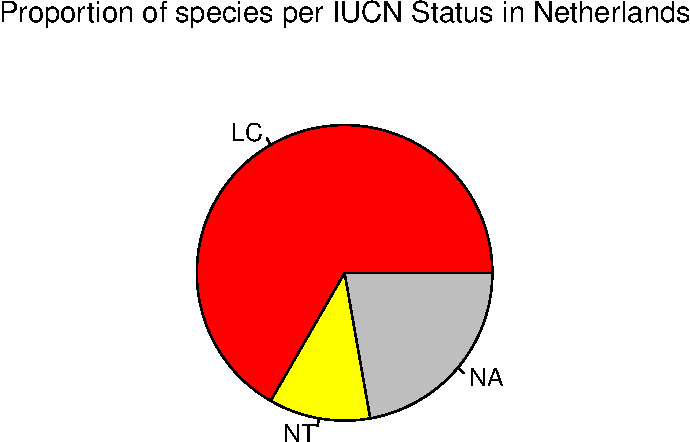
\includegraphics{esds_book_files/figure-latex/unnamed-chunk-134-1.pdf}
***
\#\#\# Cleaning data with IUCN Status

In this part of the tutorial, we have to clean the data that we will use for the correlations. We have provided the dataset already with the IUCN status since the code needs a lot of time to run, but the procedure is exactly the same as we did in the previous sections. So, let us load the dataset, it's called \emph{datasetIUCN}.

In the previous sections, we saw that for some species we did not have information on the IUCN status. In these cases, we set the IUCN status as NA. We can check for possible NA values by calling the \texttt{unique()} function.

\begin{Shaded}
\begin{Highlighting}[]
\NormalTok{dataset_IUCN <-}\StringTok{ }\KeywordTok{read_csv}\NormalTok{(}\StringTok{"./data/datasetIUCN.csv"}\NormalTok{)}
\KeywordTok{unique}\NormalTok{(dataset_IUCN}\OperatorTok{$}\NormalTok{IUCN)}
\end{Highlighting}
\end{Shaded}

\begin{verbatim}
##  [1] "LC" "CR" "lc" "VU" NA   "EX" "NT" "DD" "EN" "EW"
\end{verbatim}

\textbf{Checkpoint}
Now your task is to remove the row with the IUCN status as NA. You can use the function \texttt{subset()} to get the subset of the dataset with information about the IUCN status.

\begin{Shaded}
\begin{Highlighting}[]
\CommentTok{# your code}
\end{Highlighting}
\end{Shaded}

\textbf{Solution}

\begin{Shaded}
\begin{Highlighting}[]
\CommentTok{# subset the data without NAs (!=NA; not equal to NA), so this effectively removes NAs}
\NormalTok{dataset_IUCN_NA <-}\StringTok{ }\KeywordTok{subset}\NormalTok{(dataset_IUCN, dataset_IUCN}\OperatorTok{$}\NormalTok{IUCN }\OperatorTok{!=}\StringTok{ "NA"}\NormalTok{)}

\CommentTok{# check if it worked}
\KeywordTok{unique}\NormalTok{(dataset_IUCN_NA}\OperatorTok{$}\NormalTok{IUCN)}
\end{Highlighting}
\end{Shaded}

\begin{verbatim}
## [1] "LC" "CR" "lc" "VU" "EX" "NT" "DD" "EN" "EW"
\end{verbatim}

Next, we will load the shapefile of glacial basins using the package \texttt{rgdal} and the function \texttt{readOGR()}. We fetch the data from different fish basins across Europe in the \texttt{basin\_shapefile} from the data stored in the basins folder. In order to plot the basins on the map we will use \texttt{fortify()} function on the \texttt{basin\_shapefile}. This function helps to convert a lines-and-points object into a data frame for ggplot. We will store this dataframe as \texttt{fort\_basin}.

\begin{Shaded}
\begin{Highlighting}[]
\NormalTok{basin_shapefile <-}\StringTok{ }\KeywordTok{readOGR}\NormalTok{(}\StringTok{"./data/basins"}\NormalTok{)}
\end{Highlighting}
\end{Shaded}

\begin{verbatim}
## OGR data source with driver: ESRI Shapefile 
## Source: "/Users/pascalschneider/Polybox/Shared/Data Science Lecture Planning - shared folder/4 Datasets/basins", layer: "basins"
## with 3119 features
## It has 9 fields
\end{verbatim}

\begin{Shaded}
\begin{Highlighting}[]
\NormalTok{fort_basin <-}\StringTok{ }\KeywordTok{fortify}\NormalTok{(basin_shapefile)}
\KeywordTok{head}\NormalTok{(fort_basin)}
\end{Highlighting}
\end{Shaded}

\begin{verbatim}
##        long       lat order  hole piece id group
## 1 -43.00000 -22.55000     1 FALSE     1  0   0.1
## 2 -43.03750 -22.69583     2 FALSE     1  0   0.1
## 3 -43.05325 -22.69523     3 FALSE     1  0   0.1
## 4 -43.05507 -22.68816     4 FALSE     1  0   0.1
## 5 -43.06888 -22.68693     5 FALSE     1  0   0.1
## 6 -43.07279 -22.68390     6 FALSE     1  0   0.1
\end{verbatim}

We can visualise our \texttt{basin\_shapefile} using \texttt{ggplot()}.

\begin{Shaded}
\begin{Highlighting}[]
\KeywordTok{ggplot}\NormalTok{() }\OperatorTok{+}\StringTok{ }\KeywordTok{geom_polygon}\NormalTok{(}\DataTypeTok{data =}\NormalTok{ fort_basin, }\KeywordTok{aes}\NormalTok{(}\DataTypeTok{x =}\NormalTok{ long, }\DataTypeTok{y =}\NormalTok{ lat, }\DataTypeTok{group =}\NormalTok{ group), }\DataTypeTok{colour =} \StringTok{"black"}\NormalTok{, }\DataTypeTok{fill =} \OtherTok{NA}\NormalTok{)}
\end{Highlighting}
\end{Shaded}

\textbackslash begin\{figure\}
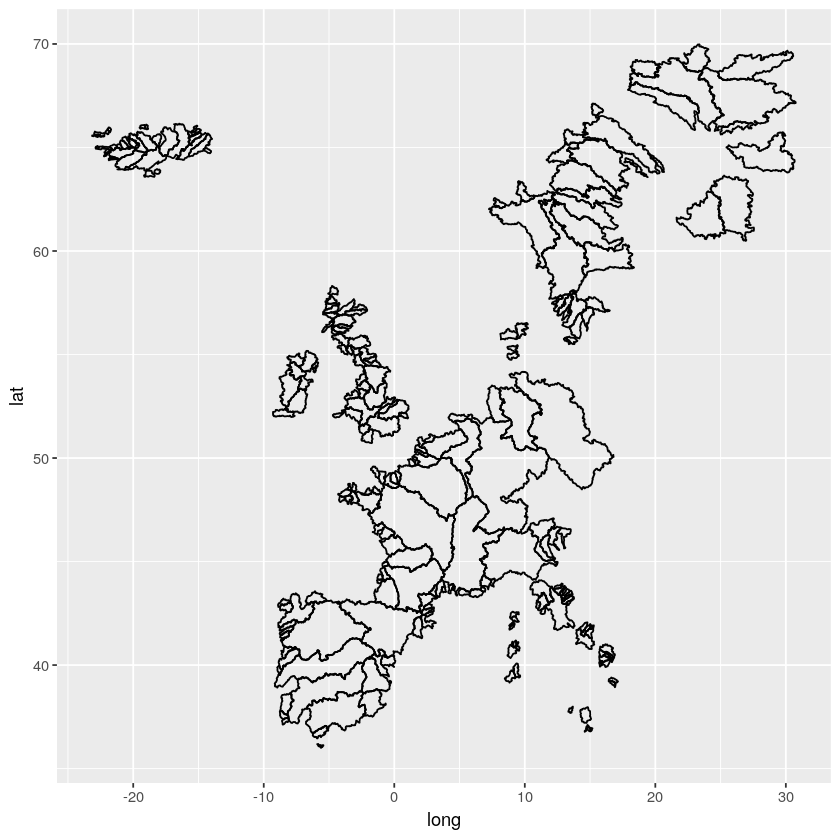
\includegraphics[width=11.67in]{./figures/output_186_0} \textbackslash caption\{Plot of \texttt{fort\_basin}.\}\label{fig:europe}
\textbackslash end\{figure\}

\begin{center}\rule{0.5\linewidth}{0.5pt}\end{center}

\hypertarget{maps-of-species-richness-and-red-list-species-proportions}{%
\subsection{Maps of species richness and Red List species proportions}\label{maps-of-species-richness-and-red-list-species-proportions}}

\hypertarget{preparing-data}{%
\subsubsection*{Preparing data}\label{preparing-data}}
\addcontentsline{toc}{subsubsection}{Preparing data}

We now want to map the species richness and Red List species proportions. Let us first calculate the species richness and proportion of Red List species per basin. Species richness is the number of species pro basin and the proportion of red list species is the ratio between the number of species in the red list and the number of species pro basin. We will iterate over the vector with the basin names and we will use the function \texttt{nrow()} to find the number of occurrences.

\begin{Shaded}
\begin{Highlighting}[]
\ControlFlowTok{for}\NormalTok{ (x }\ControlFlowTok{in} \KeywordTok{as.character}\NormalTok{(basin_shapefile}\OperatorTok{$}\NormalTok{BasinName)) \{}
    
  \CommentTok{# we now restrict to dataset to the basin x}
\NormalTok{  dataset_basins <-}\StringTok{ }\NormalTok{dataset_IUCN[dataset_IUCN}\OperatorTok{$}\NormalTok{X1.Basin.Name}\OperatorTok{==}\NormalTok{x,]}
    
  \CommentTok{# number of species in the given country x}
\NormalTok{  n1 <-}\StringTok{ }\KeywordTok{nrow}\NormalTok{(dataset_basins)}
    
  \CommentTok{# we now restrict to dataset to the country x and Red List}
\NormalTok{  dataset_c_IUCN <-}\StringTok{ }\NormalTok{dataset_basins[}\KeywordTok{grep}\NormalTok{(}\StringTok{"VU|EN|EX|EW|CR"}\NormalTok{, dataset_basins}\OperatorTok{$}\NormalTok{IUCN),] }
    
  \CommentTok{# number of species in the given country x with given IUCN Status}
\NormalTok{  n2 <-}\StringTok{ }\KeywordTok{nrow}\NormalTok{(dataset_c_IUCN)}
    
  \CommentTok{# compute the proportion }
\NormalTok{  basin_shapefile}\OperatorTok{$}\NormalTok{proportion[basin_shapefile}\OperatorTok{$}\NormalTok{BasinName}\OperatorTok{==}\NormalTok{x] <-}\StringTok{ }\NormalTok{n2}\OperatorTok{/}\NormalTok{n1}
\NormalTok{  basin_shapefile}\OperatorTok{$}\NormalTok{richness[basin_shapefile}\OperatorTok{$}\NormalTok{BasinName}\OperatorTok{==}\NormalTok{x] <-}\StringTok{ }\NormalTok{n1  }
\NormalTok{\}}
\end{Highlighting}
\end{Shaded}

We can see the newly computed data for the columns \emph{`proportion'} and \emph{`richness'} with respect to each basin in the \texttt{basin\_shapefile}.

\begin{Shaded}
\begin{Highlighting}[]
\KeywordTok{head}\NormalTok{(basin_shapefile}\OperatorTok{@}\NormalTok{data)}
\end{Highlighting}
\end{Shaded}

\begin{verbatim}
##       BasinName   Country Ecoregion Endorheic Out_Longit  Out_Latit Med_Longit
## 0  Cachoeirinha    Brazil Neotropic      <NA>  -43.10344 -22.693658  -43.06899
## 1      Comprido    Brazil Neotropic      <NA>  -47.07734 -24.451571  -47.15300
## 2 Arroyo.Walker Argentina Neotropic      <NA>  -62.29922 -40.628898  -62.59625
## 3     Aconcagua     Chile Neotropic      <NA>  -71.53604 -32.912822  -70.65645
## 4        Amazon    Brazil Neotropic      <NA>  -52.23409  -1.619426  -64.57286
## 5      Andalien     Chile Neotropic      <NA>  -73.09136 -36.664541  -72.81968
##    Med_Latit    Surf_area proportion richness
## 0 -22.595111     228.8151        NaN        0
## 1 -24.465831     204.7977        NaN        0
## 2 -40.507344     969.1561        NaN        0
## 3 -32.770645    7318.8768        NaN        0
## 4  -6.714857 5888416.9156        NaN        0
## 5 -36.824925     767.4691        NaN        0
\end{verbatim}

Next we get the map of Europe. We will read the data in \texttt{continent\_shapefile} and then will extract the continent `Europe' map. If you call the variable \texttt{europe} you will see that the dataframe is empty. This is because it extracts only the map data which we can simply plot by passing the europe as an argument in \texttt{plot()} function. We will do it in the upcoming code cells.

\begin{Shaded}
\begin{Highlighting}[]
\NormalTok{continents <-}\StringTok{ }\KeywordTok{readOGR}\NormalTok{(}\StringTok{'./data/continent_shapefile'}\NormalTok{)}
\end{Highlighting}
\end{Shaded}

\begin{verbatim}
## OGR data source with driver: ESRI Shapefile 
## Source: "/Users/pascalschneider/Polybox/Shared/Data Science Lecture Planning - shared folder/4 Datasets/continent_shapefile", layer: "continent"
## with 8 features
## It has 1 fields
\end{verbatim}

\begin{Shaded}
\begin{Highlighting}[]
\NormalTok{europe <-}\StringTok{ }\NormalTok{continents[continents}\OperatorTok{$}\NormalTok{CONTINENT }\OperatorTok{==}\StringTok{ 'Europe'}\NormalTok{,]}
\end{Highlighting}
\end{Shaded}

\begin{verbatim}
Warning message in readOGR("../data/continent_shapefile"):
“First layer europe_map read; multiple layers present in
/work/04_data_scraping/data/continent_shapefile, check layers with ogrListLayers()”


OGR data source with driver: ESRI Shapefile 
Source: "/work/04_data_scraping/data/continent_shapefile", layer: "europe_map"
with 53 features
It has 94 fields
\end{verbatim}

\hypertarget{plotting-data}{%
\subsubsection*{Plotting data}\label{plotting-data}}
\addcontentsline{toc}{subsubsection}{Plotting data}

So now let us plot the proportions of Red List species. First, we will create a new column \emph{`proportion\_colour'} and in this column, we will store the colours. Then we will break the proportions into 10 different parts by grouping the values in the proportion column into 10 using the \texttt{cut()} function. Then we get rid of the index vector using \texttt{as.numeric()} and get all the values as numeric values. We used the \texttt{rev()} function to reverse the colours, red colour indicates the species that are getting distinct and have very less proportion pro basin and yellow indicates the species with comparatively more proportion in the basin. Finally, we store these colours to the column proportion\_colour. The colour indicates the proportion of Red List species occurring in the corresponding basin. We do the same for the species richness.

\begin{Shaded}
\begin{Highlighting}[]
\NormalTok{basin_shapefile}\OperatorTok{$}\NormalTok{proportion_colour <-}\StringTok{ }\KeywordTok{rev}\NormalTok{(}\KeywordTok{heat.colors}\NormalTok{(}\DecValTok{11}\NormalTok{))[}\KeywordTok{as.numeric}\NormalTok{(}\KeywordTok{cut}\NormalTok{(basin_shapefile}\OperatorTok{$}\NormalTok{proportion, }\DataTypeTok{breaks =} \DecValTok{10}\NormalTok{))]}
\end{Highlighting}
\end{Shaded}

Now we create a new column in the \emph{fort\_basin} dataframe and map the values of \emph{`proportion\_colour'} into the new color column. We are doing this to have the colour (species proportion divided into 10 parts) and lat-long values in one datframe which helps to plot the graph using \texttt{ggplot()}. Remember, above we extracted the continent \emph{`europe'} from the \texttt{continent\_shapefile}, here we will use \texttt{fortiy()} on the europe dataset to plot it. In detail, we will plot the \texttt{fort\_europe} and \texttt{fort\_basin} data on the map.

\begin{Shaded}
\begin{Highlighting}[]
\NormalTok{fort_basin}\OperatorTok{$}\NormalTok{color <-}\StringTok{ }\NormalTok{fort_basin}\OperatorTok{$}\NormalTok{id   }\CommentTok{# create a new column color}

\ControlFlowTok{for}\NormalTok{ (i }\ControlFlowTok{in} \KeywordTok{as.numeric}\NormalTok{(}\KeywordTok{unique}\NormalTok{(fort_basin}\OperatorTok{$}\NormalTok{id)))\{   }\CommentTok{# map the values into color column by id}
\NormalTok{   fort_basin}\OperatorTok{$}\NormalTok{color[fort_basin}\OperatorTok{$}\NormalTok{id }\OperatorTok{==}\StringTok{ }\NormalTok{i] <-}\StringTok{ }\NormalTok{basin_shapefile}\OperatorTok{@}\NormalTok{data}\OperatorTok{$}\NormalTok{proportion_colour[i}\OperatorTok{+}\DecValTok{1}\NormalTok{]}
\NormalTok{\}}

\NormalTok{fort_europe <-}\StringTok{ }\KeywordTok{fortify}\NormalTok{(europe)}
\end{Highlighting}
\end{Shaded}

\begin{Shaded}
\begin{Highlighting}[]
\KeywordTok{ggplot}\NormalTok{(fort_basin, }\KeywordTok{aes}\NormalTok{(}\DataTypeTok{x =}\NormalTok{ long, }\DataTypeTok{y =}\NormalTok{ lat, }\DataTypeTok{group =}\NormalTok{ group)) }\OperatorTok{+}
\StringTok{  }\KeywordTok{geom_polygon}\NormalTok{(}\DataTypeTok{data =}\NormalTok{ fort_europe, }\KeywordTok{aes}\NormalTok{(}\DataTypeTok{x =}\NormalTok{ long, }\DataTypeTok{y =}\NormalTok{ lat, }\DataTypeTok{group =}\NormalTok{ group), }\DataTypeTok{colour =} \StringTok{'white'}\NormalTok{) }\OperatorTok{+}
\StringTok{  }\KeywordTok{geom_polygon}\NormalTok{(}\DataTypeTok{fill =}\NormalTok{ fort_basin}\OperatorTok{$}\NormalTok{color, }\DataTypeTok{colour =} \StringTok{"black"}\NormalTok{)}\OperatorTok{+}
\StringTok{  }\KeywordTok{xlim}\NormalTok{(}\OperatorTok{-}\DecValTok{25}\NormalTok{, }\DecValTok{28}\NormalTok{)}
\end{Highlighting}
\end{Shaded}

\begin{figure}
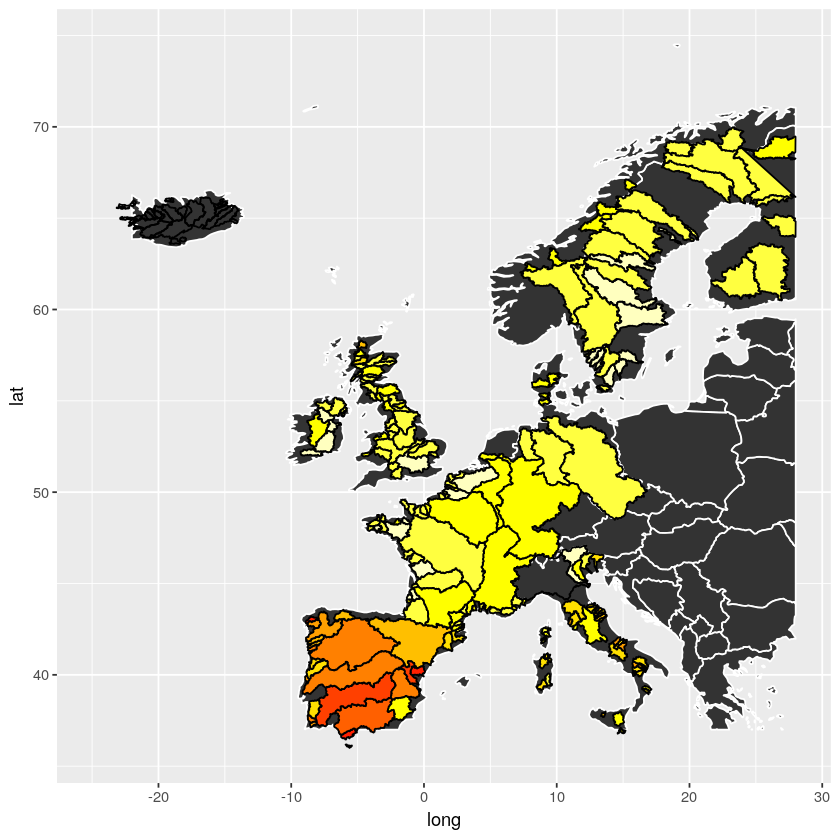
\includegraphics[width=11.67in]{./figures/output_201_0} \caption{Proportions of Red List species in Europe.}\label{fig:europe2}
\end{figure}

From the Figure \ref{fig:europe2}, we see that the proportion of Red List species is highest in South-Western Europe. The aim of the Red List is to inform decision-makers about potentially endangered species, i.e.~species whose population size has been rapidly declining during the last decades or the species that only occur in small numbers at present. The proportion of species on the Red List of each region, therefore, gives an indication of the risk of species going extinct in a region and represents an important tool for conservation strategies.

\hypertarget{repeat-for-mapping-species-richness}{%
\subsubsection*{Repeat for mapping species richness}\label{repeat-for-mapping-species-richness}}
\addcontentsline{toc}{subsubsection}{Repeat for mapping species richness}

We will repeat the above steps all together for plotting the species richness on map.

\begin{Shaded}
\begin{Highlighting}[]
\CommentTok{# break the richness  of the species into 10 parts and then we assign colors to each part }
\NormalTok{basin_shapefile}\OperatorTok{$}\NormalTok{richness_colour <-}\StringTok{ }\KeywordTok{rev}\NormalTok{(}\KeywordTok{heat.colors}\NormalTok{(}\DecValTok{11}\NormalTok{))[}\KeywordTok{as.numeric}\NormalTok{(}\KeywordTok{cut}\NormalTok{(basin_shapefile}\OperatorTok{$}\NormalTok{richness, }\DataTypeTok{breaks =} \DecValTok{10}\NormalTok{))]}

\NormalTok{fort_basin}\OperatorTok{$}\NormalTok{rich_color <-}\StringTok{ }\NormalTok{fort_basin}\OperatorTok{$}\NormalTok{id    }\CommentTok{# create a new column rich_color}

\CommentTok{# mapping the values from basin_shapefile to fort_basin}

\ControlFlowTok{for}\NormalTok{ (i }\ControlFlowTok{in} \KeywordTok{as.numeric}\NormalTok{(}\KeywordTok{unique}\NormalTok{(fort_basin}\OperatorTok{$}\NormalTok{id))) }
\NormalTok{\{}
\NormalTok{   fort_basin}\OperatorTok{$}\NormalTok{rich_color[fort_basin}\OperatorTok{$}\NormalTok{id }\OperatorTok{==}\StringTok{ }\NormalTok{i] <-}\StringTok{ }\NormalTok{basin_shapefile}\OperatorTok{@}\NormalTok{data}\OperatorTok{$}\NormalTok{richness_colour[i}\OperatorTok{+}\DecValTok{1}\NormalTok{]}
\NormalTok{\}}

\CommentTok{# plot}
\KeywordTok{ggplot}\NormalTok{(fort_basin, }\KeywordTok{aes}\NormalTok{(}\DataTypeTok{x =}\NormalTok{ long, }\DataTypeTok{y =}\NormalTok{ lat, }\DataTypeTok{group =}\NormalTok{ group)) }\OperatorTok{+}
\StringTok{  }\KeywordTok{geom_polygon}\NormalTok{(}\DataTypeTok{data =}\NormalTok{ fort_europe, }\KeywordTok{aes}\NormalTok{(}\DataTypeTok{x =}\NormalTok{ long, }\DataTypeTok{y =}\NormalTok{ lat, }\DataTypeTok{group =}\NormalTok{ group), }\DataTypeTok{colour =} \StringTok{'white'}\NormalTok{) }\OperatorTok{+}
\StringTok{  }\KeywordTok{geom_polygon}\NormalTok{(}\DataTypeTok{fill =}\NormalTok{ fort_basin}\OperatorTok{$}\NormalTok{rich_color, }\DataTypeTok{colour =} \StringTok{"black"}\NormalTok{)}\OperatorTok{+}
\StringTok{  }\KeywordTok{xlim}\NormalTok{(}\OperatorTok{-}\DecValTok{25}\NormalTok{, }\DecValTok{28}\NormalTok{)}
\end{Highlighting}
\end{Shaded}

\begin{figure}
\includegraphics[width=11.67in]{./figures/output_204_0} \caption{Species richness in Europe.}\label{fig:europe3}
\end{figure}

\hypertarget{relation-of-basin-size-and-species-richness}{%
\subsection{Relation of basin size and species richness}\label{relation-of-basin-size-and-species-richness}}

In the previous section, you observed the spatial patterns of fish diversity across Europe. In this section, we will try to explain these patterns. To achieve this, we will correlate the fish species richness of each basin to the surface area of the corresponding area to see how the species richness varies with respect to the surface area of the basin. We begin with plotting a simple scatterplot. We will log transform the data we have on surface area as it helps to make data conform to normality and also helps to deal with the outliers and skeweness in the data. Then we will plot this data against species richness. Since the data-deficient basins show zero observations in the dataframe, we will remove those first.

Now we will create a new dataframe with the \emph{surface area} and \emph{richness}. We'll rename the columns as \emph{`Basin\_area'} and \emph{`Species\_richness'} respectively. We make a simple scatterplot with a regression line to visualise the relationship.

\begin{Shaded}
\begin{Highlighting}[]
\NormalTok{basin_shapefile <-}\StringTok{ }\NormalTok{basin_shapefile[basin_shapefile}\OperatorTok{$}\NormalTok{richness}\OperatorTok{!=}\DecValTok{0}\NormalTok{,]}

\NormalTok{bs_sr <-}\StringTok{ }\KeywordTok{tibble}\NormalTok{(basin_shapefile}\OperatorTok{@}\NormalTok{data}\OperatorTok{$}\NormalTok{Surf_area, basin_shapefile}\OperatorTok{@}\NormalTok{data}\OperatorTok{$}\NormalTok{richness )}
\KeywordTok{names}\NormalTok{(bs_sr)[}\DecValTok{1}\NormalTok{]<-}\StringTok{ 'Basin_area'}
\KeywordTok{names}\NormalTok{(bs_sr)[}\DecValTok{2}\NormalTok{]<-}\StringTok{ 'Species_richness'}

\KeywordTok{ggplot}\NormalTok{(bs_sr, }\KeywordTok{aes}\NormalTok{(}\DataTypeTok{x =} \KeywordTok{log}\NormalTok{(Basin_area), }\DataTypeTok{y =}\NormalTok{ Species_richness)) }\OperatorTok{+}
\KeywordTok{geom_point}\NormalTok{() }\OperatorTok{+}
\KeywordTok{geom_smooth}\NormalTok{(}\DataTypeTok{method=}\StringTok{'lm'}\NormalTok{, }\DataTypeTok{color=}\StringTok{"red"}\NormalTok{, }\DataTypeTok{size=}\FloatTok{0.5}\NormalTok{, }\DataTypeTok{se=}\OtherTok{FALSE}\NormalTok{)}\OperatorTok{+}
\KeywordTok{xlab}\NormalTok{(}\StringTok{"Basin Area"}\NormalTok{) }\OperatorTok{+}
\KeywordTok{ylab}\NormalTok{(}\StringTok{"Species Richness"}\NormalTok{) }\OperatorTok{+}
\KeywordTok{theme_classic}\NormalTok{()}
\end{Highlighting}
\end{Shaded}

\begin{verbatim}
## `geom_smooth()` using formula 'y ~ x'
\end{verbatim}

\includegraphics{esds_book_files/figure-latex/unnamed-chunk-147-1.pdf}

The plot shows a positive correlation between basin area and fish richness, meaning that we expect to see a higher richness in larger basins. This pattern is commonly observed in ecology and one explanation for this is that larger areas provide different habitat types (niches), which allows more species to co-exist.

As a next step, we will create a simple model of this relationship. This allows us to make predictions on the richness of fish species in other basins based on the basin area.

\begin{Shaded}
\begin{Highlighting}[]
\NormalTok{richness_model <-}\StringTok{ }\KeywordTok{lm}\NormalTok{(richness}\OperatorTok{~}\KeywordTok{log}\NormalTok{(Surf_area), }\DataTypeTok{data=}\NormalTok{basin_shapefile}\OperatorTok{@}\NormalTok{data) }\CommentTok{#create a linear model}
\end{Highlighting}
\end{Shaded}

We now want to calculate the confidence intervals of the model to have a better idea of the uncertainty of the model. We will then coerce the basin surface, the model fit and the confidence interval into a new data frame called \emph{model\_df}.

\begin{Shaded}
\begin{Highlighting}[]
\CommentTok{#calculate the confidence intervals}
\NormalTok{model_df <-}\StringTok{ }\KeywordTok{as.data.frame}\NormalTok{(}\KeywordTok{cbind}\NormalTok{(}\KeywordTok{log}\NormalTok{(basin_shapefile}\OperatorTok{$}\NormalTok{Surf_area), }\KeywordTok{predict}\NormalTok{(richness_model, }\DataTypeTok{interval=}\StringTok{'confidence'}\NormalTok{)))}
\KeywordTok{names}\NormalTok{(model_df)[}\DecValTok{1}\NormalTok{] <-}\StringTok{ 'log_area'}
\KeywordTok{head}\NormalTok{(model_df)}
\end{Highlighting}
\end{Shaded}

\begin{verbatim}
##     log_area      fit      lwr      upr
## 174 8.274449 28.39050 26.57731 30.20369
## 291 9.960755 37.89576 35.13808 40.65343
## 335 7.949240 26.55739 24.82776 28.28701
## 340 5.953703 15.30907 13.07901 17.53914
## 392 9.074369 32.89944 30.71907 35.07981
## 393 5.538369 12.96794 10.47659 15.45930
\end{verbatim}

The final step is to plot the model fit and prediction intervals over the data. To get nice lines in the plot, the \emph{model\_df} dataframe needs to be ordered by the basin area first.

\begin{Shaded}
\begin{Highlighting}[]
\KeywordTok{ggplot}\NormalTok{(bs_sr, }\KeywordTok{aes}\NormalTok{(}\DataTypeTok{x =} \KeywordTok{log}\NormalTok{(Basin_area), }\DataTypeTok{y =}\NormalTok{ Species_richness)) }\OperatorTok{+}
\KeywordTok{geom_point}\NormalTok{() }\OperatorTok{+}
\KeywordTok{geom_line}\NormalTok{(}\KeywordTok{aes}\NormalTok{(}\DataTypeTok{x =}\NormalTok{ model_df}\OperatorTok{$}\NormalTok{log_area, }\DataTypeTok{y=}\NormalTok{ model_df}\OperatorTok{$}\NormalTok{fit ), }\DataTypeTok{color =} \StringTok{"red"}\NormalTok{)}\OperatorTok{+}
\KeywordTok{geom_line}\NormalTok{(}\KeywordTok{aes}\NormalTok{(}\DataTypeTok{x =}\NormalTok{ model_df}\OperatorTok{$}\NormalTok{log_area, }\DataTypeTok{y=}\NormalTok{ model_df}\OperatorTok{$}\NormalTok{lwr ), }\DataTypeTok{color =} \StringTok{"red"}\NormalTok{, }\DataTypeTok{linetype =} \StringTok{"dotted"}\NormalTok{)}\OperatorTok{+}
\KeywordTok{geom_line}\NormalTok{(}\KeywordTok{aes}\NormalTok{(}\DataTypeTok{x =}\NormalTok{ model_df}\OperatorTok{$}\NormalTok{log_area, }\DataTypeTok{y=}\NormalTok{ model_df}\OperatorTok{$}\NormalTok{upr ), }\DataTypeTok{color =} \StringTok{"red"}\NormalTok{, }\DataTypeTok{linetype =} \StringTok{"dotted"}\NormalTok{)}\OperatorTok{+}
\KeywordTok{xlab}\NormalTok{(}\StringTok{"Basin Area"}\NormalTok{) }\OperatorTok{+}
\KeywordTok{ylab}\NormalTok{(}\StringTok{"Species Richness"}\NormalTok{) }\OperatorTok{+}
\KeywordTok{theme_classic}\NormalTok{()}
\end{Highlighting}
\end{Shaded}

\includegraphics{esds_book_files/figure-latex/unnamed-chunk-150-1.pdf}

\begin{center}\rule{0.5\linewidth}{0.5pt}\end{center}

\textbf{Checkpoint}
You have now seen how you can calculate and plot the confidence interval of your data. Based on your model you can also create a so-called \textbf{prediction interval} which gives an estimate of the range in which the model will most likely predict the y-values (for a given x-value). In our case the prediction interval would indicate in which range the model would expect the fish richness to be for a given basin surface area. Do you think that these prediction intervals will be broader or narrower than the confidence interval? Try to write the code for calculating and plotting the prediction intervals by yourself.

\begin{Shaded}
\begin{Highlighting}[]
\CommentTok{# your code}
\end{Highlighting}
\end{Shaded}

\textbf{Solution}

\begin{Shaded}
\begin{Highlighting}[]
\CommentTok{#prediction intervals}

\CommentTok{# make a dataframe of area and richness model predictions}
\NormalTok{model_df_prediction <-}\StringTok{ }\KeywordTok{as.data.frame}\NormalTok{(}\KeywordTok{cbind}\NormalTok{(}\KeywordTok{log}\NormalTok{(basin_shapefile}\OperatorTok{$}\NormalTok{Surf_area), }\KeywordTok{predict}\NormalTok{(richness_model, }\DataTypeTok{interval=}\StringTok{'prediction'}\NormalTok{)))}
\KeywordTok{names}\NormalTok{(model_df_prediction)[}\DecValTok{1}\NormalTok{] <-}\StringTok{ 'log_area'} 

\CommentTok{# order the basins by size}
\NormalTok{model_df_prediction <-}\StringTok{ }\NormalTok{model_df_prediction[}\KeywordTok{order}\NormalTok{(model_df_prediction}\OperatorTok{$}\NormalTok{log_area),]}

\CommentTok{# plot the model}
\KeywordTok{plot}\NormalTok{(}\KeywordTok{log}\NormalTok{(basin_shapefile}\OperatorTok{$}\NormalTok{Surf_area), basin_shapefile}\OperatorTok{$}\NormalTok{richness, }\DataTypeTok{pch=}\DecValTok{16}\NormalTok{, }\DataTypeTok{cex=}\DecValTok{1}\NormalTok{, }\DataTypeTok{col=}\KeywordTok{rgb}\NormalTok{(}\DecValTok{0}\NormalTok{,}\DecValTok{0}\NormalTok{,}\DecValTok{0}\NormalTok{,}\FloatTok{0.6}\NormalTok{), }\DataTypeTok{xlab=}\StringTok{'Basin area'}\NormalTok{, }\DataTypeTok{ylab=}\StringTok{'Basin species richness'}\NormalTok{)}
\KeywordTok{lines}\NormalTok{(model_df_prediction}\OperatorTok{$}\NormalTok{log_area, model_df_prediction}\OperatorTok{$}\NormalTok{fit, }\DataTypeTok{col=}\StringTok{'skyblue3'}\NormalTok{, }\DataTypeTok{lwd=}\DecValTok{2}\NormalTok{)}
\KeywordTok{lines}\NormalTok{(model_df_prediction}\OperatorTok{$}\NormalTok{log_area, model_df_prediction}\OperatorTok{$}\NormalTok{lwr, }\DataTypeTok{col=}\StringTok{'skyblue2'}\NormalTok{, }\DataTypeTok{lwd=}\DecValTok{2}\NormalTok{, }\DataTypeTok{lty=}\DecValTok{3}\NormalTok{)}
\KeywordTok{lines}\NormalTok{(model_df_prediction}\OperatorTok{$}\NormalTok{log_area, model_df_prediction}\OperatorTok{$}\NormalTok{upr, }\DataTypeTok{col=}\StringTok{'skyblue2'}\NormalTok{, }\DataTypeTok{lwd=}\DecValTok{2}\NormalTok{, }\DataTypeTok{lty=}\DecValTok{3}\NormalTok{)}
\end{Highlighting}
\end{Shaded}

\includegraphics{esds_book_files/figure-latex/unnamed-chunk-152-1.pdf}

\begin{center}\rule{0.5\linewidth}{0.5pt}\end{center}

\hypertarget{references}{%
\section{References}\label{references}}

\begin{itemize}
\tightlist
\item
  Automated Data Collection with R, S. Munzert, C. Rubba, P. Meißner and D. Nyhuis
\item
  XML and Web Technologies for Data Sciences with R, D. Nolan, D. Temple Lang
\item
  \url{http://www.columbia.edu/~cjd11/charles_dimaggio/DIRE/styled-4/styled-6/code-13/}
\item
  \url{https://ourcodingclub.github.io/tutorials/webscraping/}
\item
  \url{https://www.earthdatascience.org/courses/earth-analytics/get-data-using-apis/use-twitter-api-r/}
\end{itemize}

\begin{center}\rule{0.5\linewidth}{0.5pt}\end{center}

\hypertarget{exercise}{%
\section{Exercise}\label{exercise}}

For this week's exercise open up the Rstudio environment. Remember to save all your changes to this notebook using git status, git add , git commit -m ``your comment'', git push.

Today's exercise is about getting data from the web and extracting useful insights from it.

Get in touch with your teaching assistant if you have any further questions.

\hypertarget{catch-up}{%
\chapter{Catch-up}\label{catch-up}}

TBC

\hypertarget{supervised-machine-learning-basics-i}{%
\chapter{Supervised machine learning basics I}\label{supervised-machine-learning-basics-i}}

\hypertarget{introduction-2}{%
\section{Introduction}\label{introduction-2}}

\hypertarget{learning-objectives-1}{%
\subsection{Learning objectives}\label{learning-objectives-1}}

After this learning unit, you will be able to \ldots{}

\begin{itemize}
\tightlist
\item
  Differentiate machine learning from classical programming
\item
  Describe the different variants of machine learning
\item
  Conceptualize model training as an optimization problem
\item
  Describe overfitting and how it can be measured (training vs.~validation error).
\item
  Formulate a model in R.
\item
  Discuss why, when, and how to pre-process data.
\item
  Measure and minimize loss for regression and classification (video)
\item
  Describe the fundamentals of gradient descent (video)
\end{itemize}

\hypertarget{important-points-from-the-lecture}{%
\subsection{Important points from the lecture}\label{important-points-from-the-lecture}}

Machine learning refers to a class of algorithms that automatically generate statistical models of data.

There are two main types of machine learning:

\textbf{\emph{Unsupervised machine learning}}:
A class of algorithms that automatically detect patterns in data without using labels or `learning without a teacher'.\\
Examples are: PCAs, clustering, autoencoders, self-organizing maps, etc.

\textbf{\emph{Supervised machine learning}}:
A class of algorithms that automatically learn an input-output function based on example input-output pairs.\\
Examples include: support vector machines, random forests, decision trees, neural networks, etc.
Supervised machine learning requires three ingredients:
(1) Input data (2) Output data (3) A measure of model performance (a.k.a. ``loss'')

\emph{Loss} is a concept central to many supervised machine learning algorithms. It measures how well our predicted model values fit the actual observed model values, a higher value indicates a higher loss, essentially meaning the model fits less well. Ideally, loss should be minimised.
Loss can be used to update our model parameters in the next iteration of model training, this is called learning.

Supervised machine learning be used for regression (predict a continuous label) or classification (predict a categorical label).

Essentially, supervised machine learning is an optimization problem, which searches a vast and high dimensional solution space.

\hypertarget{tutorial-1}{%
\section{Tutorial}\label{tutorial-1}}

Machine learning (ML) may appear magical. The ability of ML algorithms to detect patterns and make predictions is fascinating. However, several challenges have to be met in the process of formulating, training, and evaluating the models. In this practical we will discuss some basics of supervised ML and how to achieve best predictive results.

In general, the aim of supervised ML is to find a model \(\hat{Y} = f(X)\) that is \emph{trained} (calibrated) using observed relationships between a set of \emph{features} (also known as \emph{predictors}, or \emph{labels}, or \emph{independent variables}) \(X\) and the \emph{target} variable \(Y\). Note, that \(Y\) is observed. The hat on \(\hat{Y}\) denotes an estimate. Some algorithms can even handle predictions of multiple target variables simultaneously (e.g., neural networks). ML algorithms consist of (more or less) flexible mathematical models with a certain structure and set of parameters. At the simple extreme end of the model spectrum is the univariate linear regression. You may not want to call this a ML algorithm because there is no iterative learning involved. Nevertheless, also univariate linear regression provides a prediction \(\hat{Y} = f(X)\), just like other (proper) ML algorithms do. The functional form of a linear regression is not particularly flexible (just a straight line for the best fit between predictors and targets) and it has only two parameters (slope and intercept). At the other extreme end are, for example, deep neural networks. They are extremely flexible, can learn highly non-linear relationships and deal with interactions between a large number of predictors. They also contain very large numbers of parameters, typically on the order of thousands. You can imagine that this allows these types of algorithms to very effectively learn from the data, but also bears the risk of \emph{overfitting}.

What is overfitting? The following example illustrates it. Let's assume that there is some true underlying relationship between a predictor \(x\) and the target variable \(y\). We don't know this relationship (in the code below, this is \texttt{true\_fun()}) and the observations contain a (normally distributed) error (\texttt{y\ =\ true\_fun(x)\ +\ 0.1\ *\ rnorm(n\_samples)}). Based on our training data (\texttt{df\_train}), we fit three polynomial models of degree 1, 4, and 15 to the observations. A polynomial of degree N is given by:
\[
y = \sum_{n=0}^N a_n x^n
\]
\(a_n\) are the coefficients, i.e., model parameters. The goal of the training is to get the coefficients \(a_n\). From the above definition, the polynomial of degree 15 has 16 parameters, while the polynomial of degree 1 has two parameters (and corresponds to a simple linear regression). You can imagine that the polynomial of degree 15 is much more flexible and should thus yield the closest fit to the training data. This is indeed the case.

\includegraphics{./figures/training.png}

We can use the same fitted models on unseen data - the \emph{validation data}. This is what's done below. Again, the same true underlying relationship is used, but we sample a new set of data points in x and add a new sample of errors on top of the true relationship.

\includegraphics{./figures/validation.png}

You see that, using the validation set, we find that ``poly4'' actually performs the best - it has a much lower RMSE that ``poly15''. Apparently, ``poly15'' was overfitted. Apparently, it indeed used its flexibility to fit not only the shape of the true underlying relationship, but also the observation errors on top of it. This has obviously the implication that, when this model is used to make predictions for data that was not used for training (calibration), it will yield misguided predictions that are affected by the errors in the training set. In the above pictures we can also conclude that ``poly1'' was underfitted.

It gets even worse when applying the fitted polynomial models to data that extends beyond the range in \(x\) that was used for model training. Here, we're extending just 20\% to the right.

\includegraphics{./figures/validation_extrapolation.png}

You see that the RMSE for ``poly15'' literally explodes. The model is hopelessly overfitted and completely useless for prediction, although it looked like it fit the data best when we considered at the training results. This is a fundamental challenge in ML - finding the model with the best \emph{generalisability}. That is, a model that not only fits the training data well, but also performs well on unseen data.

The phenomenon of fitting/overfitting as a function of the model ``flexibility'' is also referred to as \emph{bias vs.~variance trade-off}. The bias describes how well a model matches the training set (average error). A model with low bias will match the data set closely and vice versa. The variance describes how much a model changes when you train it using different portions of your data set. ``poly15'' has a high variance, but much of its variance is the result of misled training on observation errors. On the other extreme, ``poly1'' has a high bias. It's not affected by the noise in observations, but its predictions are also far off the observations. In ML, we are challenged to balance this trade-off. In the next figure you can see a schematic illustration of the bias--variance trade-off.

\includegraphics{./figures/bias-variance.png}

This chapter introduces the methods to achieve the best model generalisability and find the sweet spot between high bias and high variance. The steps to get there include the preprocessing of data, splitting the data into training and testing sets, and model training that ``steers'' the model towards what is considered a good model fit in terms of its generalisation power.

You have learned in video 6a about the basic setup of supervised ML, with input data containing the features (or predictors) \(X\), predicted (\(\hat{Y}\)) and observed target values (\(Y\), also known as \emph{labels}). In video 6b (title 6c: loss and it's minimization), you learned about the loss function which quantifies the agreement between \(Y\) and \(\hat{Y}\) and defines the objective of the model training. Here, you'll learn how all of this can be implemented in R. Depending on your application or research question, it may also be of interest to evaluate the relationships embodied in \(f(X)\) or to quantify the importance of different predictors in our model. This is referred to as \emph{model interpretation} and is introduced in the respectively named subsection. Finally, we'll get into \emph{feature selection} in the next Application session.

The topic of supervised machine learning methods covers enough material to fill two sessions. Therefore, we split this part in two. Model training, implementing the an entire modelling workflow, model evaluation and interpretation will be covered in the next session's tutorial (Supervised Machine Learning Methods II).

Of course, a plethora of algorithms exist that do the job of \(Y = f(X)\). Each of them has its own strengths and limitations. It is beyond the scope of this course to introduce a larger number of ML algorithms. Subsequent sessions will focus primarily on Artificial Neural Networks (ANN) - a type of ML algorithm that has gained popularity for its capacity to efficiently learn patterns in large data sets. For illustration purposes in this and the next chapter, we will briefly introduce two simple alternative ``ML'' methods, linear regression and K-nearest-neighbors. They have quite different characteristics and are therefore great for illustration purposes in this chapter.

\textbf{Checkpoint}

What can you say about the bias and the variance of the following graphs?

\includegraphics{./figures/bias-variance_2.png}

\textbf{Solution}

In the righthand figure we can see a low bias and a high variance. While in the left figure we see a high bias and a low variance.

We can now load some packages that we will use in this tutorial.

\begin{Shaded}
\begin{Highlighting}[]
\KeywordTok{library}\NormalTok{(tidyverse)}
\KeywordTok{library}\NormalTok{(ggplot2)}
\KeywordTok{library}\NormalTok{(modelr)}
\KeywordTok{library}\NormalTok{(forcats)}
\KeywordTok{library}\NormalTok{(yardstick)}
\KeywordTok{library}\NormalTok{(recipes)}
\KeywordTok{library}\NormalTok{(caret)}
\KeywordTok{library}\NormalTok{(broom)}
\end{Highlighting}
\end{Shaded}

\hypertarget{linear-regression}{%
\subsection{Linear regression}\label{linear-regression}}

\textbf{Theory}

In its simplest form, the univariate linear regression, we assume a linear relationship between \(X\) and \(Y\):
\[
Y_i = \beta_0 + \beta_1 X_i + \epsilon_i, \;\;\; i = 1, 2, ...n \;,
\]
where \(Y_i\) is the i-th observation of the target variable, and \(X_i\) is the i-th value of the (single) predictor variable. The errors \(\epsilon_i\) are assumed to be independent from each other (no autocorrelation), normally distributed, have mean of zero and a constant variance. \(\beta_0\) and \(\beta_1\) are constant coefficients (model parameters). Fitting a linear regression is finding the values for \(\beta_0\) and \(\beta_1\) so that the sum of the square errors is minimized, that is:
\[
\sum_i \epsilon_i^2 = \sum_i (Y_i - \beta_0 - \beta_1 X_i)^2 = \text{min}.
\]

Since the expected value of \(\epsilon\) is zero (because it's normally distributed with mean zero), predictions of a linear regression model are obtained by \(Y_\text{new} = \beta_0 + \beta_1 X_\text{new}\).

It's not hard to imagine that the univariate linear regression can be generalized to a multivariate linear regression, where we assume that the target variable is a linear combination of \(p\) predictor variables:
\[
Y = \beta_0 + \beta_1 X_1 + \beta_2 X_2 + \; ... \; + \beta_p X_p + \epsilon \;.
\]
Note that here, \(X\), \(Y\), and \(\epsilon\) are vectors of length corresponding to the number of observations in our data set (\(n\) - as above). Analogously, calibrating the \(p\) coefficients \(\beta_1, \beta_2, ..., \beta_p\) is to minimize the sum of square errors \(\sum_i \epsilon_i^2\). While the regression is a line in two-dimensional space for the univariate case, it is a plane in three-dimensional space for bi-variate regression, and so on.

\textbf{Implementation}

To fit a univariate linear regression model in R, we can use the \texttt{lm()} function. Already in Chapter 2, we made linear models by doing:

\begin{Shaded}
\begin{Highlighting}[]
\NormalTok{ddf_ch_lae <-}\StringTok{ }\KeywordTok{read_csv}\NormalTok{(}\StringTok{"./data/ddf_ch_lae.csv"}\NormalTok{) }\CommentTok{# loads 'ddf_ch_lae'}

\NormalTok{df <-}\StringTok{ }\NormalTok{ddf_ch_lae }\OperatorTok\StringTok{ }
\StringTok{  }\NormalTok{dplyr}\OperatorTok{::}\KeywordTok{select}\NormalTok{(}\OperatorTok{-}\NormalTok{NEE_VUT_REF_QC, }\OperatorTok{-}\NormalTok{TIMESTAMP) }\OperatorTok\StringTok{  }\CommentTok{# not numeric features}
\StringTok{  }\KeywordTok{drop_na}\NormalTok{() }
\end{Highlighting}
\end{Shaded}

\begin{Shaded}
\begin{Highlighting}[]
\NormalTok{linmod1 <-}\StringTok{ }\KeywordTok{lm}\NormalTok{(GPP_NT_VUT_REF }\OperatorTok{~}\StringTok{ }\NormalTok{PPFD_IN, }\DataTypeTok{data =}\NormalTok{ df)}
\end{Highlighting}
\end{Shaded}

Here, \texttt{GPP\_NT\_VUT\_REF} is \(Y\), and \texttt{PPFD\_IN} is \(X\). We can include multiple predictors for a multivariate regression, for example as:

\begin{Shaded}
\begin{Highlighting}[]
\NormalTok{linmod2 <-}\StringTok{ }\KeywordTok{lm}\NormalTok{(GPP_NT_VUT_REF }\OperatorTok{~}\StringTok{ }\NormalTok{PPFD_IN }\OperatorTok{+}\StringTok{ }\NormalTok{VPD_F }\OperatorTok{+}\StringTok{ }\NormalTok{TA_F, }\DataTypeTok{data =}\NormalTok{ df)}
\end{Highlighting}
\end{Shaded}

or all available features in our data set (all columns other than \texttt{GPP\_NT\_VUT\_REF} in \texttt{df}) as:

\begin{Shaded}
\begin{Highlighting}[]
\NormalTok{linmod3 <-}\StringTok{ }\KeywordTok{lm}\NormalTok{(GPP_NT_VUT_REF }\OperatorTok{~}\StringTok{ }\NormalTok{., }\DataTypeTok{data =}\NormalTok{ df)}
\end{Highlighting}
\end{Shaded}

\texttt{linmod} is now a model object of class \texttt{"lm"}. It is a list containing the following components:

\begin{Shaded}
\begin{Highlighting}[]
\KeywordTok{ls}\NormalTok{(linmod1)}
\end{Highlighting}
\end{Shaded}

\begin{verbatim}
##  [1] "assign"        "call"          "coefficients"  "df.residual"  
##  [5] "effects"       "fitted.values" "model"         "qr"           
##  [9] "rank"          "residuals"     "terms"         "xlevels"
\end{verbatim}

Enter \texttt{?lm} in the console for a complete documentation of these components.

R offers a set of generic functions that work with this type of object. The following returns a human-readable report of the fit.

\begin{Shaded}
\begin{Highlighting}[]
\KeywordTok{summary}\NormalTok{(linmod1)}
\end{Highlighting}
\end{Shaded}

\begin{verbatim}
## 
## Call:
## lm(formula = GPP_NT_VUT_REF ~ PPFD_IN, data = df)
## 
## Residuals:
##      Min       1Q   Median       3Q      Max 
## -10.1392  -1.9090  -0.1295   1.7981  14.9231 
## 
## Coefficients:
##              Estimate Std. Error t value Pr(>|t|)    
## (Intercept) 0.9201659  0.0813886   11.31   <2e-16 ***
## PPFD_IN     0.0144372  0.0002275   63.46   <2e-16 ***
## ---
## Signif. codes:  0 '***' 0.001 '**' 0.01 '*' 0.05 '.' 0.1 ' ' 1
## 
## Residual standard error: 2.929 on 3631 degrees of freedom
## Multiple R-squared:  0.5258, Adjusted R-squared:  0.5257 
## F-statistic:  4027 on 1 and 3631 DF,  p-value: < 2.2e-16
\end{verbatim}

We can also extract coefficients \(\beta\) with

\begin{Shaded}
\begin{Highlighting}[]
\KeywordTok{coef}\NormalTok{(linmod1)}
\end{Highlighting}
\end{Shaded}

\begin{verbatim}
## (Intercept)     PPFD_IN 
##   0.9201659   0.0144372
\end{verbatim}

Under the assumption of normally distributed errors \(\epsilon\) with mean zero and constant variance \(\sigma^2\), the magnitude of the variance can be estimated by

\[
\widehat{\sigma}^2 = \frac{1}{n-p} \sum_{i=1}^n \epsilon_i^2
\]
- \(\widehat{\sigma}^2\) is also referred to as the \emph{mean square error} (MSE), and its root,
- \(\widehat{\sigma}\) is the \emph{root mean square error} (RMSE).

The RMSE can be extracted from the linear regression model object by:

\begin{Shaded}
\begin{Highlighting}[]
\KeywordTok{sigma}\NormalTok{(linmod1)}
\end{Highlighting}
\end{Shaded}

\begin{verbatim}
## [1] 2.929148
\end{verbatim}

The RMSE is also reported in the output of \texttt{summary()} as the \texttt{Residual\ standard\ error}. The MSE can be calculated accordingly as:

\begin{Shaded}
\begin{Highlighting}[]
\KeywordTok{sigma}\NormalTok{(linmod1)}\OperatorTok{^}\DecValTok{2}
\end{Highlighting}
\end{Shaded}

\begin{verbatim}
## [1] 8.579907
\end{verbatim}

Although \texttt{summary()} provides a nice, human-readable output, you may find it unpractical to work with. A set of relevant quantities are returned in a tidy format using \texttt{tidy()} from the broom package:

\begin{Shaded}
\begin{Highlighting}[]
\KeywordTok{library}\NormalTok{(broom)}
\KeywordTok{tidy}\NormalTok{(linmod1)}
\end{Highlighting}
\end{Shaded}

\begin{verbatim}
## # A tibble: 2 x 5
##   term        estimate std.error statistic  p.value
##   <chr>          <dbl>     <dbl>     <dbl>    <dbl>
## 1 (Intercept)   0.920   0.0814        11.3 3.75e-29
## 2 PPFD_IN       0.0144  0.000228      63.5 0.
\end{verbatim}

\textbf{Model advantages and concerns}

An advantage of linear regression is that the coefficients provide information that is straight-forward to interpret. We've seen above, that \texttt{GPP\_NT\_VUT\_REF} increases by 0.014 for a unit increase in \texttt{PPFD\_IN}. Of course, the units of the coefficients depend on the units of \texttt{GPP\_NT\_VUT\_REF} and \texttt{PPFD\_IN}. This has the advantage that the data does not need to be normalised. That is, a linear regression model with the same predictive skills can be found, irrespective of whether \texttt{GPP\_NT\_VUT\_REF} is given in g Cm\(^{-2}\)s\(^{-1}\) or in kg Cm\(^{-2}\)s\(^{-1}\).

Another advantage of linear regression is that it's much less prone to overfit than other algorithms. We've seen this in the overfitting example above. But this can also be a disadvantage. Indeed, we found that the linear model ``poly1'' is rather under-fitting. It's not able to capture non-linearities in the observed relationship and exhibits a poorer performance than ``poly4'' also on the validation data set.

A further limitation is that least squares regression requires \(n>p\). In words: the number of observations must be greater than the number of predictors. If this is not given, one can resort to step-wise forward regression, where predictors are sequentially added based on which predictor adds the most additional information at each step. You'll encounter stepwise regression in the Application session 8.

When multiple predictors are linearly correlated, then linear regression cannot discern individual effects and individual predictors may appear statistically insignificant when they would be significant if covarying predicotrs were not included in the model. Such instability can get propagated to predictions. Again, stepwise regression can be used to remedy this problem. However, when one predictor covaries with multiple other predictors, this may not work. For many applications in environmental sciences, we deal with limited numbers of predictors. We can use our own knowledge to examine potentially problematic covariations and make an informed pre-selection rather than throwing all predictors we can possibly think of at our models. Such a pre-selection can be guided by the model performance on a validation data set (more on that below).

An alternative strategy is to use \emph{dimension reduction} methods. Principal Component regression reduces the data to capture only the complementary axes along which our data varies and therefore collapses covarying predictors into a single one that represents their common axis of variation. Partial Least Squares regression works similarly but modifies the principal components so that they are maximally correlated to the target variable. You can read more on their implementation in R \href{https://bradleyboehmke.github.io/HOML/linear-regression.html\#PCR}{here}.

\textbf{Checkpoint}

Considering the univariate linear regression model \texttt{GPP\_NT\_VUT\_REF\ \textasciitilde{}\ PPFD\_IN}, how do coefficients \(\beta_0\) and \(\beta_1\) change when you add 1 to all values \texttt{GPP\_NT\_VUT\_REF}?

\textbf{Solution}

\begin{Shaded}
\begin{Highlighting}[]
\KeywordTok{lm}\NormalTok{(GPP_NT_VUT_REF }\OperatorTok{~}\StringTok{ }\NormalTok{PPFD_IN, }\DataTypeTok{data =}\NormalTok{ df }\OperatorTok\StringTok{ }\KeywordTok{mutate}\NormalTok{(}\DataTypeTok{GPP_NT_VUT_REF =}\NormalTok{ GPP_NT_VUT_REF }\OperatorTok{+}\StringTok{ }\DecValTok{1}\NormalTok{))}
\end{Highlighting}
\end{Shaded}

\begin{verbatim}
## 
## Call:
## lm(formula = GPP_NT_VUT_REF ~ PPFD_IN, data = df %>% mutate(GPP_NT_VUT_REF = GPP_NT_VUT_REF + 
##     1))
## 
## Coefficients:
## (Intercept)      PPFD_IN  
##     1.92017      0.01444
\end{verbatim}

\begin{Shaded}
\begin{Highlighting}[]
\KeywordTok{lm}\NormalTok{(GPP_NT_VUT_REF }\OperatorTok{~}\StringTok{ }\NormalTok{PPFD_IN, }\DataTypeTok{data =}\NormalTok{ df)}
\end{Highlighting}
\end{Shaded}

\begin{verbatim}
## 
## Call:
## lm(formula = GPP_NT_VUT_REF ~ PPFD_IN, data = df)
## 
## Coefficients:
## (Intercept)      PPFD_IN  
##     0.92017      0.01444
\end{verbatim}

Of course, this simply corresponds to an upward shift of all points by 1, and thefore an upward shift of the regression line by 1. The slope \(\beta_1\) doesn't change, but the y-axis intercept \(\beta_0\) increases by 1.

\hypertarget{k-nearest-neighbours}{%
\subsection{K-nearest neighbours}\label{k-nearest-neighbours}}

As the name suggests, the K-nearest neighbour (KNN) uses the \(k\) observations that are ``nearest'' to the new record for which we want to make a prediction. It then calculates their average (in regression) or most frequent value (in classification) as the prediction. ``Nearest'' is determined by some distance metric evaluated based on the values of the predictors. In our example (\texttt{GPP\_NT\_VUT\_REF\ \textasciitilde{}\ .}), KNN would determine the \(k\) days where conditions, given by our set of predictors, were most similar (nearest) to the day for which we seek a prediction. Then, it calculates the prediction as the average (mean) GPP value of these days. Determining ``nearest'' neighbors is commonly based on either the Euclidean or Manhattan distances between two data points \(x_a\) and \(x_b\), considering all \(p\) predictors \(j\).
\[
\text{Euclidean: } \sqrt{ \sum_{j=1}^p (x_{a,j} - x_{b,j})^2  } \\
\text{Manhattan: } \sum_{j=1}^p | x_{a,j} - x_{b,j} |
\]

In two-dimensional space, the Euclidean distance measures the length of a straight line between two points (remember Pythagoras!). The Manhattan distance is called this way because it measures the distance you would have to walk to get from point \(a\) to point \(b\) in Manhattan, New York, where you cannot cut corners but have to follow a rectangular grid of streets. \(|x|\) is the positive value of \(x\) ( \(|-x| = x\)).

KNN is a simple algorithm that uses knowledge of the ``local'' data structure for prediction. A drawback is that the model training has to be done for each prediction step and the computation time of the training increases with \(x \times p\). KNNs are used, for example, to impute values (fill missing values) and have the advantage that predicted values are always within the range of observed values of the target variable.

To use the KNN algorithm for prediction, we have to apply two essential methods in machine learning applications: \emph{pre-processing} and \emph{hyperparameter tuning}. These are described in respective sections below.

\textbf{Checkpoint}
Compute the Euclidean metric and Manhattan distances between two points \(x_a = (1,1)\) and \(x_b = (4, 5)\).

\textbf{Solution}

\[
d_\text{Euclidean}(x_a, x_b) = \sqrt{ \sum_{j=1}^2 (x_{a,j} - x_{b,j})^2  } =  \sqrt{ (4 - 1)^2  + (5 - 1)^2} = \sqrt{25} = 5\\
d_\text{Manhattan: }(x_a, x_b) = \sum_{j=1}^2 | x_{a,j} - x_{b,j} | = |4-1|+|5-1| = 7
\]

\hypertarget{essential-methods-for-the-modelling-process}{%
\subsection{Essential methods for the modelling process}\label{essential-methods-for-the-modelling-process}}

Building a ML model is an iterative process and it is typically not possible to know which ML algorithm will perform best when you start with the process. It is also essential that you understand your data in order to apply appropriate pre-processing steps, splitting your data wisely into training and testing sets, building a robust model, and achieving an informative model evaluation. This section introduces essential methods of the modelling process that allow you to walk a safe (and hopefully still spectacular) path. This section is inspired by the fantastic tutorial \href{https://bradleyboehmke.github.io/HOML}{\emph{Hands On Machine Learning in R} by Boehmke \& Gladwell}.

\hypertarget{model-formulation}{%
\subsubsection{Model formulation}\label{model-formulation}}

Remember that the aim of supervised ML is to find a model \(\hat{Y} = f(X)\) so that \(\hat{Y}\) agrees well with observations \(Y\). We typically start with a research question where \(Y\) is given - naturally - by the problem we are addressing and we have a data set at hand where one or multiple predictors (or features) \(X\) are recorded along with \(Y\). With the data set that you have become familiar with in preceeding chapters, we have information about how GPP (ecosystem-level photosynthesis) depends on set of abiotic factors, mostly meteorological measurements. In R, it is common to use the \emph{formula} notation to specify the target and predictor variables. You have encountered formulas before, e.g., for a linear regression using the \texttt{lm()} function. To specify a linear regression model for \texttt{GPP\_NT\_VUT\_REF} with three predictors \texttt{PPFD\_IN}, \texttt{VPD\_F}, and \texttt{TA\_F}, we write:

\begin{Shaded}
\begin{Highlighting}[]
\KeywordTok{lm}\NormalTok{(GPP_NT_VUT_REF }\OperatorTok{~}\StringTok{ }\NormalTok{PPFD_IN }\OperatorTok{+}\StringTok{ }\NormalTok{VPD_F }\OperatorTok{+}\StringTok{ }\NormalTok{TA_F, }\DataTypeTok{data =}\NormalTok{ df)}
\end{Highlighting}
\end{Shaded}

Actually, the way we formulate a model is independent of the algorithm, or \emph{engine} that takes care of fitting \(f(X)\). The R package \href{https://topepo.github.io/caret/}{\textbf{caret}} provides a unified interface for using different ML algorithms implemented in separate packages. In other words, it acts as a \emph{wrapper} for multiple different model fitting, or ML algorithms. This has the advantage that it unifies the interface (the way arguments are provided). caret also provides implementations for a set of commonly used tools for data processing (which we won't use here), model training, and evaluation. We'll use caret for model training with the function \texttt{train()} (more on model training in Chapter 7). Note however, that using a specific algorithm, which is implemented in a specific package outside caret, also requires that the respective package be installed and loaded. Using caret for specifying the same linear regression model as above, using the base-R \texttt{lm()} function, can be done with caret in a generalized form as:

\begin{Shaded}
\begin{Highlighting}[]
\KeywordTok{library}\NormalTok{(caret)}
\end{Highlighting}
\end{Shaded}

\begin{Shaded}
\begin{Highlighting}[]
\KeywordTok{train}\NormalTok{(}
  \DataTypeTok{form =}\NormalTok{ GPP_NT_VUT_REF }\OperatorTok{~}\StringTok{ }\NormalTok{., }
  \DataTypeTok{data =}\NormalTok{ df, }
  \DataTypeTok{method =} \StringTok{"lm"}
\NormalTok{)}
\end{Highlighting}
\end{Shaded}

Of course, this is an overkill compared to just writing \texttt{lm(...)}. But the advantage of the unified interface is that we can simply replace the \texttt{method} argument to use a different ML algorithm. For example, to use KNN, we can write:

\begin{Shaded}
\begin{Highlighting}[]
\KeywordTok{train}\NormalTok{(}
  \DataTypeTok{form =}\NormalTok{ GPP_NT_VUT_REF }\OperatorTok{~}\StringTok{ }\NormalTok{., }
  \DataTypeTok{data =}\NormalTok{ df, }
  \DataTypeTok{method =} \StringTok{"knn"}
\NormalTok{)}
\end{Highlighting}
\end{Shaded}

Another common way of model formulation is not to use the formula notation, but to provide an argument \texttt{x} containing columns for all the predictors, and an argument \texttt{y} containing a vector of the target variable (with \texttt{length(y)\ =\ nrow(x)}). E.g., the caret function \texttt{train()} also takes such specifications:

\begin{Shaded}
\begin{Highlighting}[]
\KeywordTok{train}\NormalTok{(}
  \DataTypeTok{x =}\NormalTok{ dplyr}\OperatorTok{::}\KeywordTok{select}\NormalTok{(df, PPFD_IN, VPD_F, TA_F),}
  \DataTypeTok{y =}\NormalTok{ df}\OperatorTok{$}\NormalTok{GPP_NT_VUT_REF,}
  \DataTypeTok{method =} \StringTok{"knn"}
\NormalTok{  )}
\end{Highlighting}
\end{Shaded}

\hypertarget{data-splitting}{%
\subsubsection{Data splitting}\label{data-splitting}}

The introductory example impressively demonstrated the importance of validating the fitted model with data that was not used for training. Thus, we can test the model's generalisability. The essential step that enables us to assess the model's \emph{generalization error} is to hold out part of the data from training, and set it aside (leaving it absolutely untouched) for \emph{testing} (\emph{validation}).

There is no fixed rule for how much data are to be used for training and testing, respectively. We have to balance the trade-off between:

\begin{itemize}
\tightlist
\item
  Spending too much data for training will leave us with too little data for testing and the test results may not be robust. In this case, the sample size for getting robust validation statistics is not sufficiently large and we don't know for sure whether we are safe from an overfit model.
\item
  Spending too much data for validation will leave us with too little data for training. In this case, the ML algorithm may not be successful at finding real relationships due to insufficient amounts of training data.
\end{itemize}

Typical splits are between 60-80\% for training. However, in cases where the number of data points is very large, the gains from having more training data are marginal, but come at the cost of adding to the already high computational burden of model training.

In environmental sciences, the number of predictors is often smaller than the sample size (\(p < n\)), because its typically easier to collect repeated observations of a particular variable than to expand the set of variables being observed. Nevertheless, in cases where the number \(p\) gets large, it is important, and for some algorithms mandatory, to maintain \(p < n\) for model training.

An important aspect to consider when splitting our data is to make sure that all ``states'' of the system for which we have data are approximately equally represented in training and testing sets. This is to make sure that the algorithm learns relationships \(f(X)\) also under rare conditions \(X\), for example meteorological extreme events.

Several alternative functions for the data splitting step are available from different packages in R. Below is an example for their implementation using base R (\texttt{sample}), caret (\texttt{createDataPartition}), and rsample (\texttt{initial\_split}, combined with \texttt{training} and \texttt{testing}) and their resulting distribution of soil water content values (\texttt{SWC\_F\_MDS\_1}) in training and testing sets.

\begin{Shaded}
\begin{Highlighting}[]
\CommentTok{## using base-R}
\KeywordTok{set.seed}\NormalTok{(}\DecValTok{123}\NormalTok{) }\CommentTok{# for reproducibility}
\NormalTok{index_base <-}\StringTok{ }\KeywordTok{sample}\NormalTok{(}\DecValTok{1}\OperatorTok{:}\KeywordTok{nrow}\NormalTok{(df), }\KeywordTok{round}\NormalTok{(}\KeywordTok{nrow}\NormalTok{(df) }\OperatorTok{*}\StringTok{ }\FloatTok{0.7}\NormalTok{))}
\NormalTok{df_train_base <-}\StringTok{ }\NormalTok{df }\OperatorTok\StringTok{ }
\StringTok{  }\KeywordTok{slice}\NormalTok{(index_base)}
\NormalTok{df_test_base <-}\StringTok{ }\NormalTok{df }\OperatorTok\StringTok{ }
\StringTok{  }\KeywordTok{slice}\NormalTok{(}\OperatorTok{-}\NormalTok{index_base)}

\CommentTok{## using caret}
\KeywordTok{library}\NormalTok{(caret)}
\KeywordTok{set.seed}\NormalTok{(}\DecValTok{123}\NormalTok{)  }\CommentTok{# for reproducibility}
\NormalTok{index_caret <-}\StringTok{ }\KeywordTok{createDataPartition}\NormalTok{(df}\OperatorTok{$}\NormalTok{SWC_F_MDS_}\DecValTok{1}\NormalTok{, }\DataTypeTok{p =} \FloatTok{0.7}\NormalTok{, }\DataTypeTok{list =} \OtherTok{FALSE}\NormalTok{)}
\NormalTok{df_train_caret <-}\StringTok{ }\NormalTok{df }\OperatorTok\StringTok{ }
\StringTok{  }\KeywordTok{slice}\NormalTok{(index_caret)}
\NormalTok{df_test_caret <-}\StringTok{ }\NormalTok{df }\OperatorTok\StringTok{ }
\StringTok{  }\KeywordTok{slice}\NormalTok{(}\OperatorTok{-}\NormalTok{index_caret)}

\CommentTok{## using rsample}
\KeywordTok{library}\NormalTok{(rsample)}
\KeywordTok{set.seed}\NormalTok{(}\DecValTok{123}\NormalTok{)  }\CommentTok{# for reproducibility}
\NormalTok{split_rsample <-}\StringTok{ }\KeywordTok{initial_split}\NormalTok{(df, }\DataTypeTok{prop =} \FloatTok{0.7}\NormalTok{)}
\NormalTok{df_train_rsample <-}\StringTok{ }\KeywordTok{training}\NormalTok{(split_rsample)}
\NormalTok{df_test_rsample <-}\StringTok{ }\KeywordTok{testing}\NormalTok{(split_rsample)}
\end{Highlighting}
\end{Shaded}

\includegraphics{./figures/datasplitting.png}

In this example, you can see that not in all cases, data with very low soil water content values are sufficiently represented in the testing set (see red curve for `base R'). It may be critical to have extreme values both in the testing and training sets, e.g., if we are interested to capture responses of our target variable to very dry soil conditions. A way to control for this aspect and achieve a more similar representation of data in training and testing sets across all values, we can apply a \emph{stratified sampling}. Here, we use the \texttt{initial\_split} function from the rsample package again.

\begin{Shaded}
\begin{Highlighting}[]
\NormalTok{split_rsample_strat <-}\StringTok{ }\KeywordTok{initial_split}\NormalTok{(df, }\DataTypeTok{prop =} \FloatTok{0.7}\NormalTok{, }\DataTypeTok{strata =} \StringTok{"SWC_F_MDS_1"}\NormalTok{)}
\NormalTok{df_train_rsample_strat <-}\StringTok{ }\KeywordTok{training}\NormalTok{(split_rsample_strat)}
\NormalTok{df_test_rsample_strat <-}\StringTok{ }\KeywordTok{testing}\NormalTok{(split_rsample_strat)}
\end{Highlighting}
\end{Shaded}

\includegraphics{./figures/datasplitting_strata.png}

\hypertarget{bonus}{%
\subsection{Bonus}\label{bonus}}

To generalize this and achieve a sort of ``stratification'' with respect to all predictors, we can use the \href{https://topepo.github.io/caret/data-splitting.html\#splitting-based-on-the-predictors}{\texttt{maxDissim}} function from the \textbf{caret} package (uses the \textbf{proxy} package). It samples the most dissimilar data points after an initial pick and thus achieves a good representation of the entire feature space in our training set.

\begin{Shaded}
\begin{Highlighting}[]
\KeywordTok{library}\NormalTok{(proxy)}
\KeywordTok{set.seed}\NormalTok{(}\DecValTok{123}\NormalTok{)}
\NormalTok{startSet <-}\StringTok{ }\KeywordTok{sample}\NormalTok{(}\DecValTok{1}\OperatorTok{:}\KeywordTok{nrow}\NormalTok{(df), }\DecValTok{5}\NormalTok{)   }\CommentTok{# initial pick of five}
\NormalTok{samplePool <-}\StringTok{ }\NormalTok{df[}\OperatorTok{-}\NormalTok{startSet,]}
\NormalTok{start <-}\StringTok{ }\NormalTok{df[startSet,]}
\NormalTok{index_caret <-}\StringTok{ }\KeywordTok{maxDissim}\NormalTok{(start, samplePool, }\DataTypeTok{n =} \KeywordTok{floor}\NormalTok{(}\FloatTok{0.7} \OperatorTok{*}\StringTok{ }\KeywordTok{nrow}\NormalTok{(df))}\OperatorTok{-}\DecValTok{5}\NormalTok{ )}
\end{Highlighting}
\end{Shaded}

\hypertarget{pre-processing}{%
\subsubsection{Pre-processing}\label{pre-processing}}

Skewed data, outliers, and values covering multiple orders of magnitude can create difficulties for certain ML algorithms, e.g., or KNN or neural networks. Other algorithms, like tree-based methods (e.g., Random Forest) are more robust against such issues. This section introduces pre-processing methods that enable improved ML models and prepare the data for specific needs by the ML algorithm. There is a difference between data wrangling which we learned about in Chapter 2 and pre-processing as part of the modelling workflow. Data wrangling can be considered to encompass the steps to get raw data into a format that is usable for modelling with any sort of ML algorithm. Data wrangling are the steps to prepare the data set with variable selection, removal of bad or missing data, complementing variables from different sources, and aggregating to the desired resolution or granularity (e.g., averaging over all time steps in a day, or over all replicates in a sample). In contrast, \emph{pre-processing} refers to the additional steps that are either required by the ML algorithm (examples will be given below) or the transformation of variables guided by the resulting improvement of the predictive power of the ML model.

\textbf{Target engineering}

Target engineering refers to pre-processing of the target variable. Its application can enable improved predictions, particularly for models that make assumptions about errors (e.g., normally distributed errors in linear regression) and when the target variable follows a ``special'' distribution (e.g., heavily skewed distribution, or where the target variable is a fraction that is naturally bounded by 0 and 1). A simple log-transformation of the target variable can often resolve issues with skewed distributions. An implication of a log-transformation is that errors in predicting values in the upper end of the observed range do not affect the model disproportionally compared to errors in the lower range.

In our data set of half-hourly ecosystem flux and meteorological measurements, the variable \texttt{WS\_F} (wind speed) is skewed. The target variable that we have considered so far (\texttt{GPP\_NT\_VUT\_REF}) is not skewed. In a case where we would consider \texttt{WS\_F} to be our target variable, we would thus consider applying a log-transformation.

\begin{Shaded}
\begin{Highlighting}[]
\KeywordTok{library}\NormalTok{(patchwork)  }\CommentTok{# to combine two plots into separate panels of a single plot}

\NormalTok{gg1 <-}\StringTok{ }\NormalTok{df }\OperatorTok\StringTok{ }
\StringTok{  }\KeywordTok{ggplot}\NormalTok{(}\KeywordTok{aes}\NormalTok{(}\DataTypeTok{x =}\NormalTok{ WS_F, }\DataTypeTok{y =}\NormalTok{ ..density..)) }\OperatorTok{+}
\StringTok{  }\KeywordTok{geom_histogram}\NormalTok{() }\OperatorTok{+}
\StringTok{  }\KeywordTok{labs}\NormalTok{(}\DataTypeTok{title =} \StringTok{"Original"}\NormalTok{)}

\NormalTok{gg2 <-}\StringTok{ }\NormalTok{df }\OperatorTok\StringTok{ }
\StringTok{  }\KeywordTok{ggplot}\NormalTok{(}\KeywordTok{aes}\NormalTok{(}\DataTypeTok{x =} \KeywordTok{log}\NormalTok{(WS_F), }\DataTypeTok{y =}\NormalTok{ ..density..)) }\OperatorTok{+}
\StringTok{  }\KeywordTok{geom_histogram}\NormalTok{() }\OperatorTok{+}
\StringTok{  }\KeywordTok{labs}\NormalTok{(}\DataTypeTok{title =} \StringTok{"Log-transformed"}\NormalTok{)}

\NormalTok{gg1 }\OperatorTok{+}\StringTok{ }\NormalTok{gg2   }\CommentTok{# the + is from the patchwork library}
\end{Highlighting}
\end{Shaded}

\includegraphics{esds_book_files/figure-latex/unnamed-chunk-173-1.pdf}

When defining any pre-processing step, it should be specified as a ``recipe'' or ``blueprint'', and not actually executed on the data itself before we start with the model training. Such a ``recipe'' can then be applied to any new data, while the parameters of the data pre-processing transformations are different each time. The reason for not actually executing the data transformation is \emph{data leakage}. It happens when information from the validation data somehow finds its way into the training step. Don't worry if this sounds incomprehensible. We'll learn more about it below. For now, you can focus on the types of pre-processing steps, what they do, and how they are implemented as part of a pre-processing ``recipe'' in R.

The \href{https://recipes.tidymodels.org/}{\textbf{recipes}} package offers a powerful way to specify pre-processing steps in R and is gaining traction as part of the \href{https://www.tidymodels.org/}{tidymodels} ecosystem. It allows us to sequentially build a pre-processing pipeline using the pipe (\texttt{\%\textgreater{}\%}) operator.

\begin{Shaded}
\begin{Highlighting}[]
\KeywordTok{library}\NormalTok{(recipes)}
\KeywordTok{recipe}\NormalTok{(WS_F }\OperatorTok{~}\StringTok{ }\NormalTok{., }\DataTypeTok{data =}\NormalTok{ df) }\OperatorTok\StringTok{   }\CommentTok{# it's of course non-sense to model wind speed like this}
\StringTok{  }\KeywordTok{step_log}\NormalTok{(}\KeywordTok{all_outcomes}\NormalTok{())}
\end{Highlighting}
\end{Shaded}

\begin{verbatim}
## Data Recipe
## 
## Inputs:
## 
##       role #variables
##    outcome          1
##  predictor         10
## 
## Operations:
## 
## Log transformation on all_outcomes()
\end{verbatim}

The formula, specified as an argument in the \texttt{recipe()} function, defines variable ``roles'' (in recipes-speak). What's left of the \texttt{\textasciitilde{}} is interpreted as an ``outcome'' (the target variable). By writing \texttt{\textasciitilde{}\ .}, we specify all remaining variables in the data frame as ``predictors''. As an argument in the \texttt{step\_log()} function, we write \texttt{all\_outcomes()} to declare that the log transformation is applied only to the ``outcome'' variables we specified with the formula before.

A log-transformation doesn't necessarily result in a perfect normal distribution of transformed values. The \emph{Box-Cox} can get us closer. It can be considered a generalization of the log-transformation. Values are transformed according to the following function:
\[
y(\lambda) = \begin{cases}  
\frac{Y^\lambda-1}{\lambda}, &\; y \neq 0\\ 
\log(Y),                     &\; y = 0
\end{cases}
\]
\(\lambda\) is treated as a parameter that is fitted such that the resulting distribution of values \(y\) approaches the normal distribution. To specify a Box-Cox-transformation as part of the pre-processing, we can use \texttt{step\_BoxCox()} from the recipes package. How do transformed values look like? The strict separation of the pre-processing recipe from its execution on the data also forces us to be explict about what part of the data (training vs.~validation/testing subsets) are used for determining pre-processing parameters. Let's be clear about this in the next example and apply the initial data split first here and use the training subset for the recipe.

\begin{Shaded}
\begin{Highlighting}[]
\KeywordTok{library}\NormalTok{(rsample)}
\NormalTok{split <-}\StringTok{ }\KeywordTok{initial_split}\NormalTok{(df, }\DataTypeTok{prop =} \FloatTok{0.5}\NormalTok{)}
\NormalTok{df_train <-}\StringTok{ }\KeywordTok{training}\NormalTok{(split)}
\NormalTok{df_test <-}\StringTok{ }\KeywordTok{testing}\NormalTok{(split)}

\NormalTok{recipe_example <-}\StringTok{ }\KeywordTok{recipe}\NormalTok{(WS_F }\OperatorTok{~}\StringTok{ }\NormalTok{., }\DataTypeTok{data =}\NormalTok{ df_train) }\OperatorTok
\StringTok{   }\KeywordTok{step_BoxCox}\NormalTok{(}\KeywordTok{all_outcomes}\NormalTok{())}
\end{Highlighting}
\end{Shaded}

Now, you may be frustrated by the fact that this doesn't actually transform any data, but you want to look at how values would change. There are two more steps involved to get there. This might seem a nuisance at first but their separation is actually quite beautiful and translates the conception of the pre-processing as a ``blueprint'' into the way we write the code. You'll understand why this is so useful by the end of Chapter 7.

To get the parameter of the Box-Cox-transformation (\(\lambda\)) based on the data set \texttt{df\_train}, we have to ``prepare'' the recipe.

\begin{Shaded}
\begin{Highlighting}[]
\NormalTok{prep_example <-}\StringTok{ }\KeywordTok{prep}\NormalTok{(recipe_example, }\DataTypeTok{training =}\NormalTok{ df_train) }
\end{Highlighting}
\end{Shaded}

Finally we can actually transform the data. That is, ``bake'' the prepared recipe.

\begin{Shaded}
\begin{Highlighting}[]
\NormalTok{df_baked <-}\StringTok{ }\KeywordTok{bake}\NormalTok{(prep_example, }\DataTypeTok{new_data =}\NormalTok{ df_test)}
\end{Highlighting}
\end{Shaded}

The Box-Cox-transformed data now looks like this:

\begin{Shaded}
\begin{Highlighting}[]
\NormalTok{df_baked }\OperatorTok\StringTok{ }
\StringTok{  }\KeywordTok{ggplot}\NormalTok{(}\KeywordTok{aes}\NormalTok{(}\DataTypeTok{x =}\NormalTok{ WS_F, }\DataTypeTok{y =}\NormalTok{ ..density..)) }\OperatorTok{+}
\StringTok{  }\KeywordTok{geom_histogram}\NormalTok{() }\OperatorTok{+}
\StringTok{  }\KeywordTok{labs}\NormalTok{(}\DataTypeTok{title =} \StringTok{"Box-Cox-transformed"}\NormalTok{)}
\end{Highlighting}
\end{Shaded}

\includegraphics{esds_book_files/figure-latex/unnamed-chunk-178-1.pdf}

Note that the Box-Cox-transformation can only be applied to values that are strictly positive. In our example, wind speed (\texttt{WS\_F}) is. If this is not satisfied, a Yeo-Johnson transformation can be applied.

\begin{Shaded}
\begin{Highlighting}[]
\KeywordTok{recipe}\NormalTok{(WS_F }\OperatorTok{~}\StringTok{ }\NormalTok{., }\DataTypeTok{data =}\NormalTok{ df) }\OperatorTok
\StringTok{  }\KeywordTok{step_YeoJohnson}\NormalTok{(}\KeywordTok{all_outcomes}\NormalTok{()) }
\end{Highlighting}
\end{Shaded}

\begin{verbatim}
## Data Recipe
## 
## Inputs:
## 
##       role #variables
##    outcome          1
##  predictor         10
## 
## Operations:
## 
## Yeo-Johnson transformation on all_outcomes()
\end{verbatim}

\hypertarget{standardization}{%
\subsubsection{Standardization}\label{standardization}}

Several algorithms explicitly require data to be standardized. That is, values of all predictors vary within a comparable range. The necessity of this step becomes obvious when considering KNN, where the magnitude of the distance is strongly influenced by the order of magnitude of the predictor values. To get a quick overview of the distribution of all variables (columns) in our data frame, we can use the skimr package.

\begin{Shaded}
\begin{Highlighting}[]
\KeywordTok{library}\NormalTok{(skimr)}
\KeywordTok{skim}\NormalTok{(df)}
\end{Highlighting}
\end{Shaded}

We see for example, that typical values of \texttt{PPFD\_IN} are by a factor 100 larger than values of \texttt{VPD\_F}. A distance calculated based on these raw values would therefore be strongly dominated by the difference in \texttt{PPFD\_IN} values, and differences in \texttt{VPD\_F} would hardly affect the distance. Therefore, the data must be standardized before using it with the KNN algorithm. Standardization is done, for example, by dividing each variable, that is all values in one column, by the standard deviation of that variable, and then subtracting its mean. This way, the resulting standardized values are centered around 0, and scaled such that a value of 1 means that the data point is one standard deviation above the mean of the respective variable (column). When applied to all predictors individually, the absolute values of their variations can be directly compared and only then it can be meaningfully used for determining the distance.

Also other algorithms require data to be normalised before training. A prominent example are Artificial Neural Networks.

Standardization can be done not only by centering and scaling (as described above), but also by \emph{scaling to within range}, where values are scaled such that the minimum value within each variable (column) is 0 and the maximum is 1.

Using the recipes package again, we can specify centering and scaling by two separate steps as:

\begin{Shaded}
\begin{Highlighting}[]
\NormalTok{recipe_example <-}\StringTok{ }\KeywordTok{recipe}\NormalTok{(GPP_NT_VUT_REF }\OperatorTok{~}\StringTok{ }\NormalTok{., }\DataTypeTok{data =}\NormalTok{ df_train) }\OperatorTok\StringTok{ }
\StringTok{  }\KeywordTok{step_center}\NormalTok{(}\KeywordTok{all_numeric}\NormalTok{(), }\OperatorTok{-}\KeywordTok{all_outcomes}\NormalTok{()) }\OperatorTok
\StringTok{  }\KeywordTok{step_scale}\NormalTok{(}\KeywordTok{all_numeric}\NormalTok{(), }\OperatorTok{-}\KeywordTok{all_outcomes}\NormalTok{())}
\end{Highlighting}
\end{Shaded}

Here, we used selectors to apply the recipe step to several variables at once. The first selector, \texttt{all\_numeric()}, selects all variables that are either integers or real values. The second selector, \texttt{-all\_outcomes()} removes any outcome (target) variables from this recipe step.

As seen above for the feature engineering example, this does not return a standardized version of the data frame \texttt{df\_train}, but rather the information that allows us to apply the same standardization also to other data sets. In other words, we use the distribution of values in the data set to which we applied the function (here \texttt{df\_train}) to determine the standardization (here: mean and standard deviation). As you will learn below, this is essential and critical to avoid \emph{data leakage} (where information from the testing data set leaks into the training data set).

\hypertarget{zero-variance-predictors}{%
\subsubsection{Zero-variance predictors}\label{zero-variance-predictors}}

Sometimes, the data generation process yields variables that have the same value in each observation. And sometimes this is due to failure of the measurement device or some other bug in the data collection pipeline. Either way, this may cause some algorithms to crash or become unstable. Such ``zero-variance'' predictors are usually removed altogether. The same applies also to variables with ``near-zero variance''. That is, variables where only a few unique values occur in the entire data set with a high frequency. The danger is that, when data is split into training and testing sets, the variable may effectively become a ``zero-variance'' variable within the training subset.

We can test for zero-variance or near-zero variance predictors by quantifying the following metrics:

\begin{itemize}
\tightlist
\item
  Frequency ratio: Ratio of the frequency of the most common predictor over the second most common predictor. This should be near 1 for well-behaved predictors and get very large for problematic ones.
\item
  Percent unique values: The number of unique values divided by the total number of rows in the data set (times 100). For problematic variables, this ratio gets small (approaches 1/100).
\end{itemize}

The function \texttt{nearZeroVar} of the caret package flags suspicious variables (\texttt{zeroVar\ =\ TRUE} or \texttt{nzv\ =\ TRUE}). In our data set, we don't find any:

\begin{Shaded}
\begin{Highlighting}[]
\KeywordTok{nearZeroVar}\NormalTok{(df, }\DataTypeTok{saveMetrics=} \OtherTok{TRUE}\NormalTok{)}
\end{Highlighting}
\end{Shaded}

\begin{verbatim}
##                freqRatio percentUnique zeroVar   nzv
## TA_F            1.000000      94.02697   FALSE FALSE
## SW_IN_F         1.000000      99.22929   FALSE FALSE
## LW_IN_F         1.500000      98.54115   FALSE FALSE
## VPD_F           1.125000      75.63997   FALSE FALSE
## PA_F            1.142857      53.94990   FALSE FALSE
## P_F            69.600000      59.34489   FALSE FALSE
## WS_F            1.142857      62.95073   FALSE FALSE
## CO2_F_MDS       1.000000      98.07322   FALSE FALSE
## PPFD_IN         1.000000      99.58712   FALSE FALSE
## GPP_NT_VUT_REF  1.000000      99.77980   FALSE FALSE
## USTAR           1.000000     100.00000   FALSE FALSE
\end{verbatim}

Using the recipes package, we can add a step that removes zero-variance predictors by:

\begin{Shaded}
\begin{Highlighting}[]
\NormalTok{recipe_example <-}\StringTok{ }\NormalTok{recipe_example }\OperatorTok\StringTok{ }
\StringTok{  }\KeywordTok{step_zv}\NormalTok{(}\KeywordTok{all_predictors}\NormalTok{())}
\end{Highlighting}
\end{Shaded}

\hypertarget{one-hot-encoding}{%
\subsubsection{One-hot encoding}\label{one-hot-encoding}}

For ML algorithms that require that all predictors be numerical (e.g., neural networks, or KNN), categorical predictors have to be pre-processed and converted into new numerical predictors. The most common such transformation is \emph{one-hot encoding}, where a categorical feature (predictor) that has \(N\) levels is replaced by \(N\) new features that contain either zeros or ones depending whether the value of the categorical feature corresponds to the respective column. This creates perfect collinearity between these new column, we can also drop one of them. This is referred to as \emph{dummy encoding}.
Check out the Figure from \href{https://www.kaggle.com/dansbecker/using-categorical-data-with-one-hot-encoding}{www.kaggle.com} for a one-hot encoding visualization. Using the recipes package, one-hot encoding is implemented by:

\begin{Shaded}
\begin{Highlighting}[]
\KeywordTok{recipe}\NormalTok{(GPP_NT_VUT_REF }\OperatorTok{~}\StringTok{ }\NormalTok{., }\DataTypeTok{data =}\NormalTok{ df) }\OperatorTok\StringTok{ }
\StringTok{  }\KeywordTok{step_dummy}\NormalTok{(}\KeywordTok{all_nominal}\NormalTok{(), }\DataTypeTok{one_hot =} \OtherTok{TRUE}\NormalTok{)}
\end{Highlighting}
\end{Shaded}

\begin{verbatim}
## Data Recipe
## 
## Inputs:
## 
##       role #variables
##    outcome          1
##  predictor         10
## 
## Operations:
## 
## Dummy variables from all_nominal()
\end{verbatim}

\textbf{Checkpoint}

Apply a one-hot encoding to the to the variable Species from the data set iris (from the package data sets). Load the data by \texttt{library(datasets)}. The dataset's name is \texttt{iris}. Visualize the result.

\textbf{Solution}

\begin{Shaded}
\begin{Highlighting}[]
\KeywordTok{library}\NormalTok{(datasets)}
\NormalTok{rec <-}\StringTok{ }\KeywordTok{recipe}\NormalTok{( }\OperatorTok{~}\StringTok{ }\NormalTok{., }\DataTypeTok{data =}\NormalTok{ iris) }\OperatorTok\StringTok{ }
\StringTok{  }\KeywordTok{step_dummy}\NormalTok{(Species, }\DataTypeTok{one_hot =}\NormalTok{ T) }\OperatorTok
\StringTok{  }\KeywordTok{prep}\NormalTok{(}\DataTypeTok{training =}\NormalTok{ iris)}

\KeywordTok{summary}\NormalTok{(rec)}
\end{Highlighting}
\end{Shaded}

\begin{verbatim}
## # A tibble: 7 x 4
##   variable           type    role      source  
##   <chr>              <chr>   <chr>     <chr>   
## 1 Sepal.Length       numeric predictor original
## 2 Sepal.Width        numeric predictor original
## 3 Petal.Length       numeric predictor original
## 4 Petal.Width        numeric predictor original
## 5 Species_setosa     numeric predictor derived 
## 6 Species_versicolor numeric predictor derived 
## 7 Species_virginica  numeric predictor derived
\end{verbatim}

\begin{Shaded}
\begin{Highlighting}[]
\NormalTok{rec}\OperatorTok{$}\NormalTok{template}\OperatorTok{$}\NormalTok{Species_setosa}
\end{Highlighting}
\end{Shaded}

\begin{verbatim}
##   [1] 1 1 1 1 1 1 1 1 1 1 1 1 1 1 1 1 1 1 1 1 1 1 1 1 1 1 1 1 1 1 1 1 1 1 1 1 1
##  [38] 1 1 1 1 1 1 1 1 1 1 1 1 1 0 0 0 0 0 0 0 0 0 0 0 0 0 0 0 0 0 0 0 0 0 0 0 0
##  [75] 0 0 0 0 0 0 0 0 0 0 0 0 0 0 0 0 0 0 0 0 0 0 0 0 0 0 0 0 0 0 0 0 0 0 0 0 0
## [112] 0 0 0 0 0 0 0 0 0 0 0 0 0 0 0 0 0 0 0 0 0 0 0 0 0 0 0 0 0 0 0 0 0 0 0 0 0
## [149] 0 0
## attr(,"assign")
## [1] 1 1 1
## attr(,"contrasts")
## attr(,"contrasts")$Species
## [1] "contr.treatment"
\end{verbatim}

\begin{Shaded}
\begin{Highlighting}[]
\NormalTok{rec}\OperatorTok{$}\NormalTok{template}\OperatorTok{$}\NormalTok{Species_versicolor}
\end{Highlighting}
\end{Shaded}

\begin{verbatim}
##   [1] 0 0 0 0 0 0 0 0 0 0 0 0 0 0 0 0 0 0 0 0 0 0 0 0 0 0 0 0 0 0 0 0 0 0 0 0 0
##  [38] 0 0 0 0 0 0 0 0 0 0 0 0 0 1 1 1 1 1 1 1 1 1 1 1 1 1 1 1 1 1 1 1 1 1 1 1 1
##  [75] 1 1 1 1 1 1 1 1 1 1 1 1 1 1 1 1 1 1 1 1 1 1 1 1 1 1 0 0 0 0 0 0 0 0 0 0 0
## [112] 0 0 0 0 0 0 0 0 0 0 0 0 0 0 0 0 0 0 0 0 0 0 0 0 0 0 0 0 0 0 0 0 0 0 0 0 0
## [149] 0 0
## attr(,"assign")
## [1] 1 1 1
## attr(,"contrasts")
## attr(,"contrasts")$Species
## [1] "contr.treatment"
\end{verbatim}

\begin{Shaded}
\begin{Highlighting}[]
\NormalTok{rec}\OperatorTok{$}\NormalTok{template}\OperatorTok{$}\NormalTok{Species_virginica}
\end{Highlighting}
\end{Shaded}

\begin{verbatim}
##   [1] 0 0 0 0 0 0 0 0 0 0 0 0 0 0 0 0 0 0 0 0 0 0 0 0 0 0 0 0 0 0 0 0 0 0 0 0 0
##  [38] 0 0 0 0 0 0 0 0 0 0 0 0 0 0 0 0 0 0 0 0 0 0 0 0 0 0 0 0 0 0 0 0 0 0 0 0 0
##  [75] 0 0 0 0 0 0 0 0 0 0 0 0 0 0 0 0 0 0 0 0 0 0 0 0 0 0 1 1 1 1 1 1 1 1 1 1 1
## [112] 1 1 1 1 1 1 1 1 1 1 1 1 1 1 1 1 1 1 1 1 1 1 1 1 1 1 1 1 1 1 1 1 1 1 1 1 1
## [149] 1 1
## attr(,"assign")
## [1] 1 1 1
## attr(,"contrasts")
## attr(,"contrasts")$Species
## [1] "contr.treatment"
\end{verbatim}

\hypertarget{dealing-with-missingness-and-bad-data}{%
\subsubsection{Dealing with missingness and bad data}\label{dealing-with-missingness-and-bad-data}}

Several ML algorithms require missing values to be removed. That is, if any of the cells in one row has a missing value, the entire cell gets removed. We've seen how this is implemented in Chapter 2 for example with \texttt{na.omit()} or \texttt{tidyr::drop\_na()}. Data may be missing for several reasons. Some yield random patterns of missing data, others not. In the latter case, we can speak of \emph{informative missingness} (Kuhn \& Johnson, 2003) and its information can be used for predictions. For categorical data, we may replace such data with \texttt{"none"} (instead of \texttt{NA}), while randomly missing data may be dropped altogether. Some ML algorithms (mainly tree-based methods, e.g., random forest) can handle missing values. However, when comparing the performance of alternative ML algorithms, they should be tested with the same data and removing missing data should be done beforehand.

Visualising missing data is essential for making decisions about dropping rows with missing data versus removing predictors from the model (which would imply too much data removal). The cells with missing data in a data frame can be visualised either using ggplot and \texttt{geom\_raster()} or similarly (with additional information about the percentage of missing data for each variable) with \texttt{vis\_miss()} from the \texttt{visdat} package.
Note: the code below is set to \texttt{raw} since the notebook sturggles to handle the amount of values in \emph{hhdf}. We have provided the results as images instead.

\begin{Shaded}
\begin{Highlighting}[]
\KeywordTok{load}\NormalTok{(}\StringTok{"./data/FLX_CH-Lae_FLUXNET2015_FULLSET_HH_2004-2014_1-3_CLEAN.csv"}\NormalTok{)}

\CommentTok{# DO NOT RUN THIS CODE IS NOT WORKING IN THE NOTEBOOK (or only for a max of 30000 values)}
\CommentTok{## Code from https://bradleyboehmke.github.io/HOML/engineering.html#dealing-with-missingness}
\NormalTok{hhdf }\OperatorTok
\StringTok{  }\KeywordTok{is.na}\NormalTok{() }\OperatorTok
\StringTok{  }\NormalTok{reshape2}\OperatorTok{::}\KeywordTok{melt}\NormalTok{() }\OperatorTok
\StringTok{  }\KeywordTok{ggplot}\NormalTok{(}\KeywordTok{aes}\NormalTok{(Var2, Var1, }\DataTypeTok{fill=}\NormalTok{value)) }\OperatorTok{+}
\StringTok{  }\KeywordTok{geom_raster}\NormalTok{() }\OperatorTok{+}
\StringTok{  }\KeywordTok{coord_flip}\NormalTok{() }\OperatorTok{+}
\StringTok{  }\KeywordTok{scale_y_continuous}\NormalTok{(}\OtherTok{NULL}\NormalTok{, }\DataTypeTok{expand =} \KeywordTok{c}\NormalTok{(}\DecValTok{0}\NormalTok{, }\DecValTok{0}\NormalTok{)) }\OperatorTok{+}
\StringTok{  }\KeywordTok{scale_fill_grey}\NormalTok{(}\DataTypeTok{name =} \StringTok{""}\NormalTok{,}
                  \DataTypeTok{labels =} \KeywordTok{c}\NormalTok{(}\StringTok{"Present"}\NormalTok{,}
                             \StringTok{"Missing"}\NormalTok{)) }\OperatorTok{+}
\StringTok{  }\KeywordTok{xlab}\NormalTok{(}\StringTok{"Observation"}\NormalTok{) }\OperatorTok{+}
\StringTok{  }\KeywordTok{theme}\NormalTok{(}\DataTypeTok{axis.text.y  =} \KeywordTok{element_text}\NormalTok{(}\DataTypeTok{size =} \DecValTok{100}\OperatorTok{/}\KeywordTok{ncol}\NormalTok{(df)))}

\KeywordTok{library}\NormalTok{(visdat)}
\KeywordTok{vis_miss}\NormalTok{(}
\NormalTok{  hhdf,}
  \DataTypeTok{cluster =} \OtherTok{FALSE}\NormalTok{, }
  \DataTypeTok{warn_large_data =} \OtherTok{FALSE}
\NormalTok{  )}
\end{Highlighting}
\end{Shaded}

\includegraphics{./figures/missing_data.png}

\includegraphics{./figures/missing_data_visdat.png}

The question about what is ``bad data'' and whether or when it should be removed is often critical. In Chapter 3, we've encountered quality control information in our data set (e.g., \texttt{NEE\_VUT\_REF\_QC}), and removed data that didn't satisfy our own definition of the quality criterion. Such decisions are important to keep track of and should be reported as transparently as possible in publications. In reality, where the data generation process may start in the field with actual human beings writing notes in a lab book, and where the human collecting the data is often not the same as the human writing the paper that contains that data, it's often more difficult to keep track of such decisions. As a general principle, it is advisable to design data records such that decisions made during its process remain transparent throughout all stages of the workflow and that sufficient information be collected to enable later revisions of particularly critical decisions.

Often, and particularly when humans (and more so in the case of multiple humans) collected and recorded the data, steps are necessary to make it machine-readable. For example, dates need to be formatted consistently, units need to be specified consistently, etc. An overview of common problems with bad data and their solutions is given by the \href{https://github.com/Quartz/bad-data-guide\#spelling-is-inconsistent}{Quartz Guide to Bad Data}.

\hypertarget{supervised-machine-learning-methods-ii}{%
\chapter{Supervised machine learning methods II}\label{supervised-machine-learning-methods-ii}}

\hypertarget{application-1-variable-selection}{%
\chapter{Application 1: Variable selection}\label{application-1-variable-selection}}

\hypertarget{introduction-3}{%
\section{Introduction}\label{introduction-3}}

In Chapter 7, we noted that the coefficient of determination \(R^2\) may increase even when uninformative predictors are added to a model. This will ascribe some predictive power to an uninformative predictor that is in fact misguided by its (random) correlation with the target variable. Often, we start out formulating models, not knowing beforehand what predictors should be considered and we are tempted to use them all because the full model will always yield the best \(R^2\). In such cases, we're prone to building overconfident models that perform well on the training set, but will not perform well when predicting to new data.

In this application session, we'll implement an algorithm that sequentially searches the best additional predictor to be included in our model, starting from a single one. This is called \emph{stepwise-forward} regression (see definition below). There is also \emph{stepwise-backward} regression where predictors are sequentially removed from a model that includes them all. The challenge is that we often lack the possibility to confidently assess generalisability. The effect of spuriously increasing \(R^2\) by adding uninformative predictors can be mitigated, as we noted in Chapter 7, by considering alternative metrics that penalize the number of predictors in a model. They balance the tradeoff between model complexity (number of variables in the linear regression case) and goodness of fit. Such metrics include the \emph{adjusted-}\(R^2\),the Akaike Information Criterion (AIC), or the Bayesian Information Criterion (BIC). In cases, where sufficient data is available, also cross-validation can be used for assessing the generalisability of alternative models. Here, we'll assess how these different metrics behave for a sequence of linear regression models with an increasing number of predictors. You'll learn to write code that implements an algorithm determining the order in which variables enter the model, starting from one and going up to fourteen predictors. You'll write your own stepwise-forward regression code.

Let's get started\ldots{}

\begin{center}\rule{0.5\linewidth}{0.5pt}\end{center}

\textbf{Forward stepwise regression}

\begin{enumerate}
\def\labelenumi{\arabic{enumi}.}
\item
  Let \(\mathcal{M_0}\) denote the null model, which contains no predictors.
\item
  For \(k=0,..,p-1\):

  \begin{enumerate}
  \def\labelenumii{(\alph{enumii})}
  \item
    Consider all \(p − k\) models that augment \(\mathcal{M}_k\) with one additional predictor.
  \item
    Choose the best model among these \(p − k\) models, and call it \(\mathcal{M}_{k+1}\). Here \emph{best} is defined as having the highest \(R^2\) .
  \end{enumerate}
\item
  Select a single best model from among \(\mathcal{M}_0\), . . . , \(\mathcal{M}_p\) using cross-validated prediction error, AIC, BIC, or adjusted \(R^2\).
\end{enumerate}

\begin{center}\rule{0.5\linewidth}{0.5pt}\end{center}

\hypertarget{warm-up-1-nested-for-loop}{%
\section{Warm-up 1: Nested for-loop}\label{warm-up-1-nested-for-loop}}

Given a matrix A and a vector B (see below), do the following tasks:

\begin{itemize}
\item
  Replace the missing values (\texttt{NA}) in the first row of A by the largest value of B. After using that element of B for imputing A, drop that element from the vector B and proceed with imputing the second row of A, using the (now) largest value of the updated vector B, and drop that element from B after using it for imputing A. Repeat the same procedure for all four rows in A.
\item
  After imputing (replacing) in each step, calculate the mean of the remaining values in B and record it as a single-row data frame with two columns \texttt{row\_number} and \texttt{avg}, where \texttt{row\_number} is the row number of A where the value was imputed, and \texttt{avg} is the mean of remaining values in B. As the algorithm proceeds through rows in A, sequentially bind the single-row data frame together so that after completion of the algorithm, the data frame contains four rows (corresponding to the number of rows in A).
\end{itemize}

\begin{Shaded}
\begin{Highlighting}[]
\NormalTok{A <-}\StringTok{ }\KeywordTok{matrix}\NormalTok{(}\KeywordTok{c}\NormalTok{(}\DecValTok{6}\NormalTok{, }\DecValTok{7}\NormalTok{, }\DecValTok{3}\NormalTok{, }\OtherTok{NA}\NormalTok{, }\DecValTok{15}\NormalTok{, }\DecValTok{6}\NormalTok{, }\DecValTok{7}\NormalTok{, }
              \DecValTok{8}\NormalTok{, }\DecValTok{9}\NormalTok{, }\DecValTok{12}\NormalTok{, }\DecValTok{6}\NormalTok{, }\DecValTok{11}\NormalTok{, }\OtherTok{NA}\NormalTok{, }\DecValTok{3}\NormalTok{, }
              \DecValTok{9}\NormalTok{, }\DecValTok{4}\NormalTok{, }\DecValTok{7}\NormalTok{, }\DecValTok{3}\NormalTok{, }\DecValTok{21}\NormalTok{, }\OtherTok{NA}\NormalTok{, }\DecValTok{6}\NormalTok{, }
              \DecValTok{7}\NormalTok{, }\DecValTok{19}\NormalTok{, }\DecValTok{6}\NormalTok{, }\OtherTok{NA}\NormalTok{, }\DecValTok{15}\NormalTok{, }\DecValTok{8}\NormalTok{, }\DecValTok{10}\NormalTok{),}
            \DataTypeTok{nrow =} \DecValTok{4}\NormalTok{, }\DataTypeTok{byrow =} \OtherTok{TRUE}\NormalTok{)}
\NormalTok{B <-}\StringTok{ }\KeywordTok{c}\NormalTok{(}\DecValTok{8}\NormalTok{, }\DecValTok{4}\NormalTok{, }\DecValTok{12}\NormalTok{, }\DecValTok{9}\NormalTok{, }\DecValTok{15}\NormalTok{, }\DecValTok{6}\NormalTok{)}
\end{Highlighting}
\end{Shaded}

Before implementing these tasks, try to write down a pseudo code. This is code-like text that may not be executable, but describes the structure of real code and details where and how major steps are implemented. Next, you'll need to write actual R code. For this, you will need to find answers to the following questions:

\begin{itemize}
\tightlist
\item
  How to go through each of the element in matrix?
\item
  How to detect NA value?
\item
  How to drop an element of a given value from a vector?
\item
  How to add a row to an existing data frame?
\end{itemize}

\textbf{Solution}:

\begin{Shaded}
\begin{Highlighting}[]
\KeywordTok{library}\NormalTok{(tidyverse)}

\NormalTok{summ <-}\StringTok{ }\KeywordTok{data.frame}\NormalTok{()}

\ControlFlowTok{for}\NormalTok{ (i }\ControlFlowTok{in} \DecValTok{1}\OperatorTok{:}\KeywordTok{nrow}\NormalTok{(A))\{}
  
  \ControlFlowTok{for}\NormalTok{ (j }\ControlFlowTok{in} \DecValTok{1}\OperatorTok{:}\KeywordTok{ncol}\NormalTok{(A))\{}
    
    \ControlFlowTok{if}\NormalTok{ (}\KeywordTok{is.na}\NormalTok{(A[i,j]))\{}
\NormalTok{      A[i,j] <-}\StringTok{ }\KeywordTok{max}\NormalTok{(B)}
\NormalTok{    \}}
\NormalTok{  \}}
  

\NormalTok{  B <-}\StringTok{ }\NormalTok{B[}\OperatorTok{-}\KeywordTok{which}\NormalTok{(B }\OperatorTok{==}\StringTok{ }\KeywordTok{max}\NormalTok{(B))] }\CommentTok{# update the B vector removing the biggest values}
\NormalTok{\}}

\NormalTok{  summ <-}\StringTok{ }\KeywordTok{bind_rows}\NormalTok{(summ, }\KeywordTok{data.frame}\NormalTok{(}\DataTypeTok{row_number =}\NormalTok{ i, }\DataTypeTok{avg =} \KeywordTok{mean}\NormalTok{(B)))}
  
\NormalTok{summ}
\end{Highlighting}
\end{Shaded}

\begin{verbatim}
##   row_number avg
## 1          4   5
\end{verbatim}

\hypertarget{warm-up-2-find-the-best-single-predictor}{%
\section{Warm-up 2: Find the best single predictor}\label{warm-up-2-find-the-best-single-predictor}}

The first step of a stepwise forward regression is to find the single most powerful predictor in a univariate linear regression model for the target variable \texttt{GPP\_NT\_VUT\_REF} among all fourteen available predictors in our data set (all except those of type \texttt{date} or \texttt{character}). Implement this first part of the search, using the definition of the stepwise-forward algorithm above. Remove all rows with at least one missing value before starting the predictor search.

\begin{itemize}
\tightlist
\item
  Which predictor achieves the highest \(R^2\)?
\item
  What value is the \(R^2\)?
\item
  Visualise \(R^2\) for all univariate models, ordered by their respective \(R^2\) values.
\item
  Do you note a particular pattern? Which variables yield similar \(R^2\)? How do you expect them to be included in multivariate models of the subsequent steps in the stepwise forward regression?
\end{itemize}

\emph{Hints}:

\begin{itemize}
\item
  Model structure:

  \begin{itemize}
  \tightlist
  \item
    The ``counter'' variables in the for loop can be provided as a vector, and the counter will sequentially take on the value of each element in that vector. For example: \texttt{for\ (var\ in\ all\_predictors)\{\ ...\ \}}.
  \end{itemize}
\item
  Algorithm:

  \begin{itemize}
  \item
    To record \(R^2\) values for the different models, you may start by creating an empty vector (\texttt{vec\ \textless{}-\ c()}) before the loop and then sequentially add elements to that vector inside the loop (\texttt{vec\ \textless{}-\ c(vec,\ new\_element)}). Alternatively, you can do something similar, but with a data frame (initialising with \texttt{df\_rsq\ \textless{}-\ data.frame()} before the loop, and adding rows by \texttt{df\_rsq\ \textless{}-\ bind\_rows(df\_rsq,\ data.frame(pred\ =\ predictor\_name,\ rsq\ =\ rsq\_result))} inside the loop).
  \item
    A clever way how to construct formulas dynamically is described, for example in \href{https://stackoverflow.com/questions/4951442/formula-with-dynamic-number-of-variables}{this stackoverflow post}.
  \end{itemize}
\item
  Value retrieving:

  \begin{itemize}
  \tightlist
  \item
    Extract the \(R^2\) from the linear model object: \texttt{summary(fit\_lin){[}{[}"r.squared"{]}{]}}
  \end{itemize}
\item
  Visualising:

  \begin{itemize}
  \tightlist
  \item
    Search for solutions for how to change the order of levels to be plotted yourself.
  \end{itemize}
\end{itemize}

\begin{Shaded}
\begin{Highlighting}[]
\KeywordTok{library}\NormalTok{(tidyverse)}
\CommentTok{## read CSV and drop missing values in one step}
\NormalTok{df <-}\StringTok{ }\KeywordTok{read_csv}\NormalTok{(}\StringTok{"./data/ddf_for_08_application.csv"}\NormalTok{) }\OperatorTok\StringTok{ }
\StringTok{  }\KeywordTok{drop_na}\NormalTok{()}

\CommentTok{## specify target variable}
\NormalTok{target <-}\StringTok{ 'GPP_NT_VUT_REF'}

\CommentTok{## determine predictors as all except site ID, timestamp, and the target (should be 14)}
\NormalTok{preds <-}\StringTok{ }\NormalTok{df }\OperatorTok\StringTok{ }
\StringTok{  }\NormalTok{dplyr}\OperatorTok{::}\KeywordTok{select}\NormalTok{(}\OperatorTok{-}\NormalTok{siteid, }\OperatorTok{-}\NormalTok{TIMESTAMP, }\OperatorTok{-}\NormalTok{GPP_NT_VUT_REF) }\OperatorTok\StringTok{ }
\StringTok{  }\KeywordTok{names}\NormalTok{()}

\CommentTok{## initialise an empty data frame (necessary, because otherwise we cannot use bind_rows() below)}
\NormalTok{df_rsq <-}\StringTok{ }\KeywordTok{data.frame}\NormalTok{()}
\CommentTok{# rsq_list <- c()  # alternative for vector}

\ControlFlowTok{for}\NormalTok{ (var }\ControlFlowTok{in}\NormalTok{ preds)\{}
  
  \CommentTok{## create formula dynamically}
\NormalTok{  forml <-}\StringTok{ }\KeywordTok{as.formula}\NormalTok{(}\KeywordTok{paste}\NormalTok{(target, }\StringTok{"~"}\NormalTok{, var))}
  
  \CommentTok{## fit linear model}
\NormalTok{  fit_lin <-}\StringTok{ }\KeywordTok{lm}\NormalTok{(forml, }\DataTypeTok{data =}\NormalTok{ df)}
  
  \CommentTok{## extract R2 from linear model}
\NormalTok{  rsq <-}\StringTok{ }\KeywordTok{summary}\NormalTok{(fit_lin)[[}\StringTok{"r.squared"}\NormalTok{]]}
  
  \CommentTok{## add a row to the data frame that holds the results}
\NormalTok{  df_rsq <-}\StringTok{ }\KeywordTok{bind_rows}\NormalTok{(df_rsq, }\KeywordTok{data.frame}\NormalTok{(}\DataTypeTok{pred =}\NormalTok{ var, }\DataTypeTok{rsq =}\NormalTok{ rsq))}
  
  \CommentTok{# rsq_list <- c(rsq_list,rsq)  # alternative with vector}
\NormalTok{\}}

\CommentTok{## print best single predictor and its R2}
\NormalTok{df_rsq }\OperatorTok\StringTok{ }
\StringTok{  }\KeywordTok{arrange}\NormalTok{(}\OperatorTok{-}\NormalTok{rsq) }\OperatorTok\StringTok{  }\CommentTok{# arrange by R2 in descending order (highest R2 on top)}
\StringTok{  }\KeywordTok{slice}\NormalTok{(}\DecValTok{1}\NormalTok{)           }\CommentTok{# print only the first row (with highest R2)}
\end{Highlighting}
\end{Shaded}

\begin{verbatim}
##      pred       rsq
## 1 PPFD_IN 0.5276123
\end{verbatim}

\begin{Shaded}
\begin{Highlighting}[]
\KeywordTok{library}\NormalTok{(ggplot2)}

\CommentTok{## alternative: determine the first variable to enter into our model}
\CommentTok{# preds[which.max(rsq_list)]}

\CommentTok{## use the data frame that holds the results for plotting}
\NormalTok{df_rsq }\OperatorTok\StringTok{ }
\StringTok{  }\KeywordTok{ggplot}\NormalTok{(}\KeywordTok{aes}\NormalTok{(}\DataTypeTok{x =} \KeywordTok{reorder}\NormalTok{(pred, rsq), }\DataTypeTok{y =}\NormalTok{ rsq)) }\OperatorTok{+}
\StringTok{  }\KeywordTok{geom_bar}\NormalTok{(}\DataTypeTok{stat =} \StringTok{"identity"}\NormalTok{) }\OperatorTok{+}\StringTok{ }
\StringTok{  }\KeywordTok{labs}\NormalTok{(}\DataTypeTok{y =} \KeywordTok{expression}\NormalTok{(}\KeywordTok{italic}\NormalTok{(R)}\OperatorTok{^}\DecValTok{2}\NormalTok{), }\DataTypeTok{x =} \StringTok{"Variable"}\NormalTok{) }\OperatorTok{+}
\StringTok{  }\KeywordTok{coord_flip}\NormalTok{()}
\end{Highlighting}
\end{Shaded}

\includegraphics{esds_book_files/figure-latex/unnamed-chunk-190-1.pdf}

\textbf{Solution}:

\emph{\texttt{PPFD\_IN} achieves the highest \(R^2\) value, and the corresponding \(R^2\) values is 0.5276123.}

\emph{We could see from the above plot that \texttt{LW\_IN\_F\_MDS} and \texttt{LW\_IN\_F}, \texttt{VPD\_F} and \texttt{VPD\_F\_MDS}, \texttt{SW\_IN\_F} and \texttt{SW\_IN\_F\_MDS} share basically the same \(R^2\) values. Those variables are highly correlated and are explaining the same amount of variance in the target variable. In the subsequent steps of the stepwise forward regression, since each of the two variables are highly correlated with each other, it's likely that only one of them will be selected into our final model.}

\hypertarget{full-stepwise-regression}{%
\section{Full stepwise regression}\label{full-stepwise-regression}}

Now, we take it to the next level and implement a full stepwise forward regression as described above. For each step (number of predictors \(k\)), record the following metrics: \(R^2\), \emph{adjusted-}\(R^2\), the Akaike Information Criterion (AIC), Bayesian Information Criterion (BIC), and the 5-fold cross-validation \(R^2\) and RMSE.

\begin{itemize}
\item
  Write pseudo-code for how you plan to implement the algorithm first.
\item
  Implement the algorithm in R, run it and display the order in which predictors enter the model.
\item
  Display a table with the metrics of all \(k\) steps, and the single variable, added at each step.
\end{itemize}

\emph{Hints}:

\begin{itemize}
\item
  Model structure:

  \begin{itemize}
  \tightlist
  \item
    Recall what you learned in the breakout session, you may use the same idea on this task. Try to think of the blueprint (\emph{pseudo-code}) first: How to go through different models in each forward step? How to store predictors added to the model and how to update candidate predictors?
  \end{itemize}
\item
  Algorithm:

  \begin{itemize}
  \item
    A complication is that the set of predictors is sequentially complemented at each step of the search through \(k\). You may again use \texttt{vec\ \textless{}-\ list()} to create an empty vector, and then add elements to that vector by \texttt{vec\ \textless{}-\ c(vec,\ new\_element)}.
  \item
    It may be helpful to explicitly define a set of ``candidate predictors'' that may potentially be added to the model as a vector (e.g., \texttt{preds\_candidate}), and define predictors retained in the model from the previous step in a separate vector (e.g., \texttt{preds\_retained}). In each step, search through \texttt{preds\_candidate}, select the best predictor, add it to \texttt{preds\_retained} and remove it from \texttt{preds\_candidate}.
  \item
    At each step, record the metrics and store them in a data frame for later plots. As in the first ``warm-up'' exercise, you may record metrics at each step as a single-row data frame and sequentially stack (bind) them together.
  \item
    (As above) A clever way how to construct formulas dynamically is described, for example in \href{https://stackoverflow.com/questions/4951442/formula-with-dynamic-number-of-variables}{this stackoverflow post}.
  \item
    The metrics for the \(k\) models are assessed \emph{after} the order of added variables is determined. To be able to determine the metrics, the \(k\) models can be saved by constructing a list of models and sequentially add elements to that list (\texttt{mylist{[}{[}\ name\_new\_element\ {]}{]}\ \textless{}-\ new\_element}). You can also fit the model again after determining which predictor worked best.
  \item
    Your code will most certainly have bugs at first. To debug efficiently, write code first in a simple R script and use the debugging options in RStudio (see \href{https://support.rstudio.com/hc/en-us/articles/205612627-Debugging-with-RStudio}{here}).
  \end{itemize}
\item
  Value retriving

  \begin{itemize}
  \item
    To get AIC and BIC values for a given model, use the base-R functions \texttt{AIC()} and \texttt{BIC()}.
  \item
    To get the cross-validated \(R^2\) and RMSE, use the caret function \texttt{train()} with RMSE as the loss function, and \texttt{method\ =\ "lm"} (to fit a linear regression model). Then extract the values by \texttt{trained\_model\$results\$Rsquared} and \texttt{trained\_model\$results\$RMSE}.
  \end{itemize}
\item
  Displaying:

  \begin{itemize}
  \item
    To display a table nicely as part of the RMarkdown html output, use the function \texttt{knitr::kable()}
  \item
    To avoid reordering of the list of variable names in plotting, change the type of variable names from ``character'' to ``factor'' by \texttt{pred\ \textless{}-\ factor(pred,\ levels\ =\ pred)}
  \end{itemize}
\end{itemize}

\begin{Shaded}
\begin{Highlighting}[]
\KeywordTok{library}\NormalTok{(caret)  }\CommentTok{# need train() for cross-validation}

\CommentTok{## specify target variable (as above)}
\NormalTok{target <-}\StringTok{ 'GPP_NT_VUT_REF'}

\CommentTok{## determine predictors as all except site ID, timestamp, and the target (should be 14)  (as above)}
\NormalTok{preds <-}\StringTok{ }\NormalTok{df }\OperatorTok\StringTok{ }
\StringTok{  }\NormalTok{dplyr}\OperatorTok{::}\KeywordTok{select}\NormalTok{(}\OperatorTok{-}\NormalTok{siteid, }\OperatorTok{-}\NormalTok{TIMESTAMP, }\OperatorTok{-}\NormalTok{GPP_NT_VUT_REF) }\OperatorTok\StringTok{ }
\StringTok{  }\KeywordTok{names}\NormalTok{()}

\CommentTok{# This is the vector of candidate predictors to be added in the model. To begin with, consider all as candidates.}
\NormalTok{preds_candidate <-}\StringTok{ }\NormalTok{preds }

\CommentTok{# predictors retained in the model from the previous step. To begin with, is empty.}
\NormalTok{preds_retained <-}\StringTok{ }\KeywordTok{c}\NormalTok{()}

\CommentTok{## work with lists as much as possible (more flexible!)}
\NormalTok{df_metrics <-}\StringTok{ }\KeywordTok{data.frame}\NormalTok{()}

\CommentTok{## outer loop for k predictors}
\ControlFlowTok{for}\NormalTok{ (k_index }\ControlFlowTok{in} \DecValTok{1}\OperatorTok{:}\KeywordTok{length}\NormalTok{(preds))\{}
  
  \CommentTok{# rsq_candidates <- c()}
\NormalTok{  df_rsq_candidates <-}\StringTok{ }\KeywordTok{data.frame}\NormalTok{()}
\NormalTok{  linmod_candidates <-}\StringTok{ }\KeywordTok{list}\NormalTok{()}
  
  \CommentTok{## inner loop for single additional predictor}
  \ControlFlowTok{for}\NormalTok{ (ipred }\ControlFlowTok{in}\NormalTok{ preds_candidate)\{}
    
    \CommentTok{# variable vector (new variable + retained variables) used in regression}
\NormalTok{    pred_add <-}\StringTok{ }\KeywordTok{c}\NormalTok{(preds_retained, ipred)}
    
    \CommentTok{# define formulate with newly-added predictor}
\NormalTok{    forml  <-}\StringTok{ }\KeywordTok{as.formula}\NormalTok{(}\KeywordTok{paste}\NormalTok{( target, }\StringTok{'~'}\NormalTok{, }\KeywordTok{paste}\NormalTok{(pred_add, }\DataTypeTok{collapse =} \StringTok{'+'}\NormalTok{)))}
    
    \CommentTok{# fit linear model}
\NormalTok{    fit_lin <-}\StringTok{ }\KeywordTok{lm}\NormalTok{(forml, }\DataTypeTok{data =}\NormalTok{ df)}
    
    \CommentTok{# add model object to list, and name the element according to the added variable}
\NormalTok{    linmod_candidates[[ ipred ]] <-}\StringTok{ }\NormalTok{fit_lin}
    
    \CommentTok{# record metrics for all candidates}
\NormalTok{    rsq <-}\StringTok{ }\KeywordTok{summary}\NormalTok{(fit_lin)[[}\StringTok{"r.squared"}\NormalTok{]]}
\NormalTok{    df_rsq_candidates <-}\StringTok{ }\KeywordTok{bind_rows}\NormalTok{(df_rsq_candidates, }\KeywordTok{data.frame}\NormalTok{(}\DataTypeTok{pred =}\NormalTok{ ipred, }\DataTypeTok{rsq =}\NormalTok{ rsq))  }\CommentTok{# when storing R2 in a data frame}
    \CommentTok{# rsq_candidates <- c(rsq_candidates,  rsq)  # when storing R2 as a vector}
    
\NormalTok{  \}}
  
  \CommentTok{## get name of candidate predictor that achieved the highest R2.}
\NormalTok{  pred_add <-}\StringTok{ }\NormalTok{df_rsq_candidates }\OperatorTok\StringTok{  }\CommentTok{# when storing R2 in a data frame}
\StringTok{    }\KeywordTok{arrange}\NormalTok{(}\KeywordTok{desc}\NormalTok{(rsq)) }\OperatorTok\StringTok{ }
\StringTok{    }\KeywordTok{slice}\NormalTok{(}\DecValTok{1}\NormalTok{) }\OperatorTok\StringTok{ }
\StringTok{    }\KeywordTok{pull}\NormalTok{(pred) }\OperatorTok\StringTok{ }
\StringTok{    }\KeywordTok{as.character}\NormalTok{()}
  
  \CommentTok{# pred_add <- preds_candidate[ which.max(rsq_candidates) ]   # when storing R2 as a vector}
  
  \CommentTok{## add best predictors to retained predictors }
\NormalTok{  preds_retained <-}\StringTok{ }\KeywordTok{c}\NormalTok{(preds_retained, pred_add)}
  
  \CommentTok{## get the cross-validation R2}
\NormalTok{  forml  <-}\StringTok{ }\KeywordTok{as.formula}\NormalTok{(}\KeywordTok{paste}\NormalTok{( target, }\StringTok{'~'}\NormalTok{, }\KeywordTok{paste}\NormalTok{(preds_retained, }\DataTypeTok{collapse =} \StringTok{'+'}\NormalTok{)))}
\NormalTok{  control <-}\StringTok{ }\KeywordTok{trainControl}\NormalTok{(}\DataTypeTok{method =} \StringTok{"cv"}\NormalTok{, }\DataTypeTok{number =} \DecValTok{5}\NormalTok{)}
  \KeywordTok{set.seed}\NormalTok{(}\DecValTok{123}\NormalTok{)}
  \CommentTok{# cv_modl <- train(forml, data = df, method = "lm", , metric = "Rsquared", trControl = control)}
\NormalTok{  cv_modl <-}\StringTok{ }\KeywordTok{train}\NormalTok{(forml, }\DataTypeTok{data =}\NormalTok{ df, }\DataTypeTok{method =} \StringTok{"lm"}\NormalTok{, }\DataTypeTok{metric =} \StringTok{"RMSE"}\NormalTok{, }\DataTypeTok{trControl =}\NormalTok{ control)}

  \CommentTok{# record AIC and BIC and adjusted-R2 of the respective model}
\NormalTok{  df_metrics <-}\StringTok{ }\NormalTok{df_metrics }\OperatorTok\StringTok{ }
\StringTok{    }\KeywordTok{bind_rows}\NormalTok{(}
      \KeywordTok{data.frame}\NormalTok{( }\DataTypeTok{pred =}\NormalTok{ pred_add,}
                  \DataTypeTok{rsq =} \KeywordTok{summary}\NormalTok{(linmod_candidates[[ pred_add ]])[[}\StringTok{"r.squared"}\NormalTok{]],}
                  \DataTypeTok{adj_rsq =} \KeywordTok{summary}\NormalTok{(linmod_candidates[[ pred_add ]])[[}\StringTok{"adj.r.squared"}\NormalTok{]],}
                  \DataTypeTok{cv_rsq =}\NormalTok{ cv_modl}\OperatorTok{$}\NormalTok{results}\OperatorTok{$}\NormalTok{Rsquared,}
                  \DataTypeTok{cv_rmse =}\NormalTok{ cv_modl}\OperatorTok{$}\NormalTok{results}\OperatorTok{$}\NormalTok{RMSE,}
                  \DataTypeTok{aic =} \KeywordTok{AIC}\NormalTok{(linmod_candidates[[ pred_add ]]),}
                  \DataTypeTok{bic =} \KeywordTok{BIC}\NormalTok{(linmod_candidates[[ pred_add ]])}
\NormalTok{      )}
\NormalTok{    )}
  

  \CommentTok{# remove the selected variable from the candidate variable list}
\NormalTok{  preds_candidate <-}\StringTok{ }\NormalTok{preds_candidate[}\OperatorTok{-}\KeywordTok{which}\NormalTok{(preds_candidate }\OperatorTok{==}\StringTok{ }\NormalTok{pred_add)]}
  \CommentTok{# preds_candidate <- setdiff(preds_candidate,pred_add)  # alternative}
  
\NormalTok{\}}

\KeywordTok{data.frame}\NormalTok{(df_metrics}\OperatorTok{$}\NormalTok{pred) }\CommentTok{# order in which variables enter the model}
\end{Highlighting}
\end{Shaded}

\begin{verbatim}
##    df_metrics.pred
## 1          PPFD_IN
## 2      LW_IN_F_MDS
## 3            VPD_F
## 4             WS_F
## 5      SW_IN_F_MDS
## 6        CO2_F_MDS
## 7             TA_F
## 8             PA_F
## 9         TA_F_MDS
## 10           USTAR
## 11             P_F
## 12       VPD_F_MDS
## 13         LW_IN_F
## 14         SW_IN_F
\end{verbatim}

\begin{Shaded}
\begin{Highlighting}[]
\NormalTok{df_metrics }\OperatorTok\StringTok{ }\NormalTok{knitr}\OperatorTok{::}\KeywordTok{kable}\NormalTok{()}
\end{Highlighting}
\end{Shaded}

\begin{tabular}{l|r|r|r|r|r|r}
\hline
pred & rsq & adj\_rsq & cv\_rsq & cv\_rmse & aic & bic\\
\hline
PPFD\_IN & 0.5276123 & 0.5274601 & 0.5286098 & 2.946732 & 15529.18 & 15547.30\\
\hline
LW\_IN\_F\_MDS & 0.6237535 & 0.6235110 & 0.6244311 & 2.631186 & 14824.62 & 14848.78\\
\hline
VPD\_F & 0.6482531 & 0.6479128 & 0.6488913 & 2.544541 & 14617.55 & 14647.76\\
\hline
WS\_F & 0.6640335 & 0.6636000 & 0.6644851 & 2.486970 & 14477.03 & 14513.28\\
\hline
SW\_IN\_F\_MDS & 0.6669387 & 0.6664013 & 0.6672468 & 2.476793 & 14452.07 & 14494.35\\
\hline
CO2\_F\_MDS & 0.6696209 & 0.6689811 & 0.6695521 & 2.467823 & 14428.96 & 14477.28\\
\hline
TA\_F & 0.6708789 & 0.6701350 & 0.6703978 & 2.464609 & 14419.11 & 14473.48\\
\hline
PA\_F & 0.6726644 & 0.6718185 & 0.6718171 & 2.459555 & 14404.22 & 14464.63\\
\hline
TA\_F\_MDS & 0.6730699 & 0.6721192 & 0.6642220 & 2.487336 & 14402.37 & 14468.82\\
\hline
USTAR & 0.6733802 & 0.6723246 & 0.6639334 & 2.488412 & 14401.42 & 14473.91\\
\hline
P\_F & 0.6735098 & 0.6723487 & 0.6638548 & 2.488747 & 14402.19 & 14480.72\\
\hline
VPD\_F\_MDS & 0.6735755 & 0.6723086 & 0.6624537 & 2.493879 & 14403.57 & 14488.14\\
\hline
LW\_IN\_F & 0.6736125 & 0.6722398 & 0.6623996 & 2.494079 & 14405.22 & 14495.83\\
\hline
SW\_IN\_F & 0.6736372 & 0.6721585 & 0.6620120 & 2.495602 & 14406.98 & 14503.63\\
\hline
\end{tabular}

\begin{itemize}
\tightlist
\item
  Visualise all metrics as a function of the number of predictors (add labels for the variable names of the added predictor). Highlight the best-performing model based on the respective metric. How many predictors are in the best performing model, when assessed based on each metric?
\end{itemize}

\begin{Shaded}
\begin{Highlighting}[]
\KeywordTok{library}\NormalTok{(ggplot2)}

\NormalTok{df_metrics}\OperatorTok{$}\NormalTok{pred <-}\StringTok{  }\KeywordTok{factor}\NormalTok{(df_metrics}\OperatorTok{$}\NormalTok{pred, }\DataTypeTok{levels =}\NormalTok{ df_metrics}\OperatorTok{$}\NormalTok{pred)}

\KeywordTok{ggplot}\NormalTok{() }\OperatorTok{+}
\StringTok{  }\KeywordTok{geom_point}\NormalTok{(}\DataTypeTok{data =}\NormalTok{ df_metrics, }\KeywordTok{aes}\NormalTok{(}\DataTypeTok{x =}\NormalTok{ pred, }\DataTypeTok{y =}\NormalTok{ rsq)) }\OperatorTok{+}
\StringTok{  }\KeywordTok{geom_point}\NormalTok{(}\DataTypeTok{data =} \KeywordTok{filter}\NormalTok{(df_metrics, rsq }\OperatorTok{==}\StringTok{ }\KeywordTok{max}\NormalTok{(rsq)), }\KeywordTok{aes}\NormalTok{(}\DataTypeTok{x =}\NormalTok{ pred, }\DataTypeTok{y =}\NormalTok{ rsq), }\DataTypeTok{color =} \StringTok{"red"}\NormalTok{) }\OperatorTok{+}
\StringTok{  }\KeywordTok{labs}\NormalTok{(}\DataTypeTok{title =} \KeywordTok{expression}\NormalTok{(}\KeywordTok{italic}\NormalTok{(R)}\OperatorTok{^}\DecValTok{2}\NormalTok{)) }\OperatorTok{+}\StringTok{ }
\StringTok{  }\KeywordTok{coord_flip}\NormalTok{()}
\end{Highlighting}
\end{Shaded}

\includegraphics{esds_book_files/figure-latex/unnamed-chunk-192-1.pdf}

\begin{Shaded}
\begin{Highlighting}[]
\KeywordTok{ggplot}\NormalTok{() }\OperatorTok{+}
\StringTok{  }\KeywordTok{geom_point}\NormalTok{(}\DataTypeTok{data =}\NormalTok{ df_metrics, }\KeywordTok{aes}\NormalTok{(}\DataTypeTok{x =}\NormalTok{ pred, }\DataTypeTok{y =}\NormalTok{ adj_rsq)) }\OperatorTok{+}
\StringTok{  }\KeywordTok{geom_point}\NormalTok{(}\DataTypeTok{data =} \KeywordTok{filter}\NormalTok{(df_metrics, adj_rsq }\OperatorTok{==}\StringTok{ }\KeywordTok{max}\NormalTok{(adj_rsq)), }\KeywordTok{aes}\NormalTok{(}\DataTypeTok{x =}\NormalTok{ pred, }\DataTypeTok{y =}\NormalTok{ adj_rsq), }\DataTypeTok{color =} \StringTok{"red"}\NormalTok{) }\OperatorTok{+}
\StringTok{  }\KeywordTok{labs}\NormalTok{(}\DataTypeTok{title =} \KeywordTok{expression}\NormalTok{(}\KeywordTok{paste}\NormalTok{(}\StringTok{"Adjusted-"}\NormalTok{, }\KeywordTok{italic}\NormalTok{(R)}\OperatorTok{^}\DecValTok{2}\NormalTok{))) }\OperatorTok{+}\StringTok{ }
\StringTok{  }\KeywordTok{coord_flip}\NormalTok{()}
\end{Highlighting}
\end{Shaded}

\includegraphics{esds_book_files/figure-latex/unnamed-chunk-192-2.pdf}

\begin{Shaded}
\begin{Highlighting}[]
\KeywordTok{ggplot}\NormalTok{() }\OperatorTok{+}
\StringTok{  }\KeywordTok{geom_point}\NormalTok{(}\DataTypeTok{data =}\NormalTok{ df_metrics, }\KeywordTok{aes}\NormalTok{(}\DataTypeTok{x =}\NormalTok{ pred, }\DataTypeTok{y =}\NormalTok{ cv_rsq)) }\OperatorTok{+}
\StringTok{  }\KeywordTok{geom_point}\NormalTok{(}\DataTypeTok{data =} \KeywordTok{filter}\NormalTok{(df_metrics, cv_rsq }\OperatorTok{==}\StringTok{ }\KeywordTok{max}\NormalTok{(cv_rsq)), }\KeywordTok{aes}\NormalTok{(}\DataTypeTok{x =}\NormalTok{ pred, }\DataTypeTok{y =}\NormalTok{ cv_rsq), }\DataTypeTok{color =} \StringTok{"red"}\NormalTok{) }\OperatorTok{+}
\StringTok{  }\KeywordTok{labs}\NormalTok{(}\DataTypeTok{title =} \KeywordTok{expression}\NormalTok{(}\KeywordTok{paste}\NormalTok{(}\StringTok{"Cross-validated "}\NormalTok{, }\KeywordTok{italic}\NormalTok{(R)}\OperatorTok{^}\DecValTok{2}\NormalTok{))) }\OperatorTok{+}\StringTok{ }
\StringTok{  }\KeywordTok{coord_flip}\NormalTok{()}
\end{Highlighting}
\end{Shaded}

\includegraphics{esds_book_files/figure-latex/unnamed-chunk-192-3.pdf}

\begin{Shaded}
\begin{Highlighting}[]
\KeywordTok{ggplot}\NormalTok{() }\OperatorTok{+}
\StringTok{  }\KeywordTok{geom_point}\NormalTok{(}\DataTypeTok{data =}\NormalTok{ df_metrics, }\KeywordTok{aes}\NormalTok{(}\DataTypeTok{x =}\NormalTok{ pred, }\DataTypeTok{y =}\NormalTok{ cv_rmse)) }\OperatorTok{+}
\StringTok{  }\KeywordTok{geom_point}\NormalTok{(}\DataTypeTok{data =} \KeywordTok{filter}\NormalTok{(df_metrics, cv_rmse }\OperatorTok{==}\StringTok{ }\KeywordTok{min}\NormalTok{(cv_rmse)), }\KeywordTok{aes}\NormalTok{(}\DataTypeTok{x =}\NormalTok{ pred, }\DataTypeTok{y =}\NormalTok{ cv_rmse), }\DataTypeTok{color =} \StringTok{"red"}\NormalTok{) }\OperatorTok{+}
\StringTok{  }\KeywordTok{labs}\NormalTok{(}\DataTypeTok{title =} \KeywordTok{expression}\NormalTok{(}\KeywordTok{paste}\NormalTok{(}\StringTok{"Cross-validated "}\NormalTok{, RMSE))) }\OperatorTok{+}\StringTok{ }
\StringTok{  }\KeywordTok{coord_flip}\NormalTok{()}
\end{Highlighting}
\end{Shaded}

\includegraphics{esds_book_files/figure-latex/unnamed-chunk-192-4.pdf}

\begin{Shaded}
\begin{Highlighting}[]
\KeywordTok{ggplot}\NormalTok{() }\OperatorTok{+}
\StringTok{  }\KeywordTok{geom_point}\NormalTok{(}\DataTypeTok{data =}\NormalTok{ df_metrics, }\KeywordTok{aes}\NormalTok{(}\DataTypeTok{x =}\NormalTok{ pred, }\DataTypeTok{y =}\NormalTok{ aic)) }\OperatorTok{+}
\StringTok{  }\KeywordTok{geom_point}\NormalTok{(}\DataTypeTok{data =} \KeywordTok{filter}\NormalTok{(df_metrics, aic }\OperatorTok{==}\StringTok{ }\KeywordTok{min}\NormalTok{(aic)), }\KeywordTok{aes}\NormalTok{(}\DataTypeTok{x =}\NormalTok{ pred, }\DataTypeTok{y =}\NormalTok{ aic), }\DataTypeTok{color =} \StringTok{"red"}\NormalTok{) }\OperatorTok{+}
\StringTok{  }\KeywordTok{labs}\NormalTok{(}\DataTypeTok{title =} \StringTok{"AIC"}\NormalTok{)}\OperatorTok{+}\StringTok{ }
\StringTok{  }\KeywordTok{coord_flip}\NormalTok{()}
\end{Highlighting}
\end{Shaded}

\includegraphics{esds_book_files/figure-latex/unnamed-chunk-192-5.pdf}

\begin{Shaded}
\begin{Highlighting}[]
\KeywordTok{ggplot}\NormalTok{() }\OperatorTok{+}
\StringTok{  }\KeywordTok{geom_point}\NormalTok{(}\DataTypeTok{data =}\NormalTok{ df_metrics, }\KeywordTok{aes}\NormalTok{(}\DataTypeTok{x =}\NormalTok{ pred, }\DataTypeTok{y =}\NormalTok{ bic)) }\OperatorTok{+}
\StringTok{  }\KeywordTok{geom_point}\NormalTok{(}\DataTypeTok{data =} \KeywordTok{filter}\NormalTok{(df_metrics, bic }\OperatorTok{==}\StringTok{ }\KeywordTok{min}\NormalTok{(bic)), }\KeywordTok{aes}\NormalTok{(}\DataTypeTok{x =}\NormalTok{ pred, }\DataTypeTok{y =}\NormalTok{ bic), }\DataTypeTok{color =} \StringTok{"red"}\NormalTok{) }\OperatorTok{+}
\StringTok{  }\KeywordTok{labs}\NormalTok{(}\DataTypeTok{title =} \StringTok{"BIC"}\NormalTok{)}\OperatorTok{+}\StringTok{ }
\StringTok{  }\KeywordTok{coord_flip}\NormalTok{()}
\end{Highlighting}
\end{Shaded}

\includegraphics{esds_book_files/figure-latex/unnamed-chunk-192-6.pdf}

\begin{itemize}
\tightlist
\item
  Observe which predictors are selected into the final model and which not. Why?
\end{itemize}

\emph{Solution:}
Take the best model selected by BIC as an example, \texttt{VPD\_F} is selected into the model and \texttt{VPD\_F\_MDS} is not. They won't enter the model both because they are highly correlated and when one is in, the other doesn't add information, which proves our expectation in the previous question.

\begin{itemize}
\tightlist
\item
  Whether it matters to the order of variables entering into the model which metric (i.e.~AIC, BIC or \(R^2\)) is used? Why?
\end{itemize}

\emph{Solution:}
No, it doesn't matter. For each inner loop, when deciding which variable is sequentially chosen, we compare models of the same level (i.e.~same number of variables). In this sense, model complexities for all the models are the same, and AIC/BIC only compares the goodness of fit part, which works the same as \(R^2\).

\begin{itemize}
\tightlist
\item
  Discuss your results. Which metric do you trust most? Why? Try out your algorithm without evaluating the cross-validated \(R^2\). Do you get a computational efficiency gain? Which metric comes closest to the cross-validated \(R^2\) in terms of selecting the same number predictors?
\end{itemize}

\emph{Solution:}
Cross-validated \(R^2\) is the ``gold-standard'' for assessing generalisability. However, it is computationally costly and may not provide robust results when the data set is small. Since AIC and BIC both penalise additional predictors, they both don't select the full model with 14 variables as the best model (However, it could happen that the best model selected by AIC/BIC is the full model). The BIC selects for the same number of predictors as the cross-validated \(R^2\) and RMSE, but without the disadvantage of the computational costs. It provides a conservative and apparently robust estimate for the model generalisability. Note that the order of added predictors is determined by the simple \(R^2\) and is therefore independent of the final metrics we use for choosing the best \(k\).

\hypertarget{bonus-stepwise-regression-out-of-the-box}{%
\section{Bonus: Stepwise regression out-of-the-box}\label{bonus-stepwise-regression-out-of-the-box}}

In R, you can also conduct the above variable selection procedures automatically. \texttt{regsubsets()} from leaps package provides a convenient way to do so. It does model selection by exhaustive search, including forward or backward stepwise regression.

\begin{itemize}
\tightlist
\item
  Do a stepwise forward regression using \texttt{regsubsets()}.
\item
  Create a data frame with the same metrics as above (except cross-validated \(R^2\)).
\item
  Visualise metrics as above.
\item
  Are your result consistent?
\end{itemize}

\emph{Hints}:

\begin{itemize}
\tightlist
\item
  Specify stepwise \emph{forward} by setting \texttt{method\ =\ "forward"}.
\item
  Specify the number of predictors to examine, that is all fourteen, by setting \texttt{nvmax\ =\ 14}.
\item
  AIC values of each step are stored in \texttt{summary(regfit.fwd)\$cp} and BIC values of each step are in \texttt{summary(regfit.fwd)\$bic}, etc.
\item
  Get order in which predictors \(k\) are added (which corresponds to values returned by \texttt{summary(regfit.fwd)\$bic}), by \texttt{all\_predictors{[}regfit.fwd\$vorder{[}2:15{]}-1{]}}. \texttt{vorder} is the order of variables entering into model. Note that \texttt{Intercept} is counted here as the first to enter into the model and should be removed.
\item
  To avoid reordering of the list of variable names in plotting, change the type of variable names from ``character'' to ``factor'' by \texttt{preds\_enter\ \textless{}-\ factor(preds\_enter,\ levels\ =\ preds\_enter)}
\end{itemize}

\begin{Shaded}
\begin{Highlighting}[]
\KeywordTok{library}\NormalTok{(leaps)}
\NormalTok{regfit.fwd <-}\StringTok{ }\KeywordTok{regsubsets}\NormalTok{(}\KeywordTok{as.formula}\NormalTok{(}\KeywordTok{paste}\NormalTok{(target, }\StringTok{"~"}\NormalTok{, }\KeywordTok{paste}\NormalTok{(preds,}\DataTypeTok{collapse=}\StringTok{" + "}\NormalTok{))), }\DataTypeTok{data =}\NormalTok{ df, }\DataTypeTok{method =} \StringTok{"forward"}\NormalTok{, }\DataTypeTok{nvmax =} \DecValTok{14}\NormalTok{)}
\NormalTok{reg.summary <-}\StringTok{ }\KeywordTok{summary}\NormalTok{(regfit.fwd)}

\CommentTok{# get variables in their order added to the model}
\NormalTok{preds_enter <-}\StringTok{ }\NormalTok{preds[regfit.fwd}\OperatorTok{$}\NormalTok{vorder[}\DecValTok{2}\OperatorTok{:}\DecValTok{15}\NormalTok{]}\OperatorTok{-}\DecValTok{1}\NormalTok{]}

\CommentTok{## create metrics data frame}
\NormalTok{df_metrics_auto <-}\StringTok{ }\KeywordTok{data.frame}\NormalTok{(}
  \DataTypeTok{preds =} \KeywordTok{factor}\NormalTok{(preds_enter, }\DataTypeTok{levels =}\NormalTok{ preds_enter),}
  \DataTypeTok{rsq =}\NormalTok{ reg.summary}\OperatorTok{$}\NormalTok{rsq, }
  \DataTypeTok{adj_rsq =}\NormalTok{ reg.summary}\OperatorTok{$}\NormalTok{adjr2, }
  \DataTypeTok{aic =}\NormalTok{ reg.summary}\OperatorTok{$}\NormalTok{cp, }
  \DataTypeTok{bic =}\NormalTok{ reg.summary}\OperatorTok{$}\NormalTok{bic}
\NormalTok{  )}

\KeywordTok{ggplot}\NormalTok{() }\OperatorTok{+}
\StringTok{  }\KeywordTok{geom_point}\NormalTok{(}\DataTypeTok{data =}\NormalTok{ df_metrics_auto, }\KeywordTok{aes}\NormalTok{(}\DataTypeTok{x =}\NormalTok{ preds, }\DataTypeTok{y =}\NormalTok{ rsq)) }\OperatorTok{+}
\StringTok{  }\KeywordTok{geom_point}\NormalTok{(}\DataTypeTok{data =} \KeywordTok{filter}\NormalTok{(df_metrics_auto, rsq }\OperatorTok{==}\StringTok{ }\KeywordTok{max}\NormalTok{(rsq)), }\KeywordTok{aes}\NormalTok{(}\DataTypeTok{x =}\NormalTok{ preds, }\DataTypeTok{y =}\NormalTok{ rsq), }\DataTypeTok{color =} \StringTok{"red"}\NormalTok{) }\OperatorTok{+}
\StringTok{  }\KeywordTok{labs}\NormalTok{(}\DataTypeTok{title =} \KeywordTok{expression}\NormalTok{(}\KeywordTok{italic}\NormalTok{(R)}\OperatorTok{^}\DecValTok{2}\NormalTok{)) }\OperatorTok{+}\StringTok{ }
\StringTok{  }\KeywordTok{coord_flip}\NormalTok{()}
\end{Highlighting}
\end{Shaded}

\includegraphics{esds_book_files/figure-latex/unnamed-chunk-193-1.pdf}

\begin{Shaded}
\begin{Highlighting}[]
\KeywordTok{ggplot}\NormalTok{() }\OperatorTok{+}
\StringTok{  }\KeywordTok{geom_point}\NormalTok{(}\DataTypeTok{data =}\NormalTok{ df_metrics_auto, }\KeywordTok{aes}\NormalTok{(}\DataTypeTok{x =}\NormalTok{ preds, }\DataTypeTok{y =}\NormalTok{ adj_rsq)) }\OperatorTok{+}
\StringTok{  }\KeywordTok{geom_point}\NormalTok{(}\DataTypeTok{data =} \KeywordTok{filter}\NormalTok{(df_metrics_auto, adj_rsq }\OperatorTok{==}\StringTok{ }\KeywordTok{max}\NormalTok{(adj_rsq)), }\KeywordTok{aes}\NormalTok{(}\DataTypeTok{x =}\NormalTok{ preds, }\DataTypeTok{y =}\NormalTok{ adj_rsq), }\DataTypeTok{color =} \StringTok{"red"}\NormalTok{) }\OperatorTok{+}
\StringTok{  }\KeywordTok{labs}\NormalTok{(}\DataTypeTok{title =} \KeywordTok{expression}\NormalTok{(}\KeywordTok{paste}\NormalTok{(}\StringTok{"Adjusted-"}\NormalTok{, }\KeywordTok{italic}\NormalTok{(R)}\OperatorTok{^}\DecValTok{2}\NormalTok{))) }\OperatorTok{+}\StringTok{ }
\StringTok{  }\KeywordTok{coord_flip}\NormalTok{()}
\end{Highlighting}
\end{Shaded}

\includegraphics{esds_book_files/figure-latex/unnamed-chunk-193-2.pdf}

\begin{Shaded}
\begin{Highlighting}[]
\KeywordTok{ggplot}\NormalTok{() }\OperatorTok{+}
\StringTok{  }\KeywordTok{geom_point}\NormalTok{(}\DataTypeTok{data =}\NormalTok{ df_metrics_auto, }\KeywordTok{aes}\NormalTok{(}\DataTypeTok{x =}\NormalTok{ preds, }\DataTypeTok{y =}\NormalTok{ aic)) }\OperatorTok{+}
\StringTok{  }\KeywordTok{geom_point}\NormalTok{(}\DataTypeTok{data =} \KeywordTok{filter}\NormalTok{(df_metrics_auto, aic }\OperatorTok{==}\StringTok{ }\KeywordTok{min}\NormalTok{(aic)), }\KeywordTok{aes}\NormalTok{(}\DataTypeTok{x =}\NormalTok{ preds, }\DataTypeTok{y =}\NormalTok{ aic), }\DataTypeTok{color =} \StringTok{"red"}\NormalTok{) }\OperatorTok{+}
\StringTok{  }\KeywordTok{labs}\NormalTok{(}\DataTypeTok{title =} \StringTok{"AIC"}\NormalTok{)}\OperatorTok{+}\StringTok{ }
\StringTok{  }\KeywordTok{coord_flip}\NormalTok{()}
\end{Highlighting}
\end{Shaded}

\includegraphics{esds_book_files/figure-latex/unnamed-chunk-193-3.pdf}

\begin{Shaded}
\begin{Highlighting}[]
\KeywordTok{ggplot}\NormalTok{() }\OperatorTok{+}
\StringTok{  }\KeywordTok{geom_point}\NormalTok{(}\DataTypeTok{data =}\NormalTok{ df_metrics_auto, }\KeywordTok{aes}\NormalTok{(}\DataTypeTok{x =}\NormalTok{ preds, }\DataTypeTok{y =}\NormalTok{ bic)) }\OperatorTok{+}
\StringTok{  }\KeywordTok{geom_point}\NormalTok{(}\DataTypeTok{data =} \KeywordTok{filter}\NormalTok{(df_metrics_auto, bic }\OperatorTok{==}\StringTok{ }\KeywordTok{min}\NormalTok{(bic)), }\KeywordTok{aes}\NormalTok{(}\DataTypeTok{x =}\NormalTok{ preds, }\DataTypeTok{y =}\NormalTok{ bic), }\DataTypeTok{color =} \StringTok{"red"}\NormalTok{) }\OperatorTok{+}
\StringTok{  }\KeywordTok{labs}\NormalTok{(}\DataTypeTok{title =} \StringTok{"BIC"}\NormalTok{)}\OperatorTok{+}\StringTok{ }
\StringTok{  }\KeywordTok{coord_flip}\NormalTok{()}
\end{Highlighting}
\end{Shaded}

\includegraphics{esds_book_files/figure-latex/unnamed-chunk-193-4.pdf}

\hypertarget{warm-up-2-find-the-best-single-predictor-1}{%
\section{Warm-up 2: Find the best single predictor}\label{warm-up-2-find-the-best-single-predictor-1}}

The first step of a stepwise forward regression is to find the single most powerful predictor in a univariate linear regression model for the target variable \texttt{GPP\_NT\_VUT\_REF} among all fourteen available predictors in our data set (all except those of type \texttt{date} or \texttt{character}). Implement this first part of the search, using the definition of the stepwise-forward algorithm above. Remove all rows with at least one missing value before starting the predictor search.

\begin{itemize}
\tightlist
\item
  Which predictor achieves the highest \(R^2\)?
\item
  What value is the \(R^2\)?
\item
  Visualise \(R^2\) by predictors, ordered by their respective \(R^2\) values.
\item
  Do you note a particular pattern? Which variables yield similar \(R^2\)? How do you expect them to be included in multivariate models of the subsequent steps in the stepwise forward regression?
\end{itemize}

\emph{Hints}:

\begin{itemize}
\item
  Model structure:

  \begin{itemize}
  \tightlist
  \item
    The ``counter'' variables in the for loop can be provided as a vector, and the counter will sequentially take on the value of each element in that vector. For example: \texttt{for\ (var\ in\ all\_predictors)\{\ ...\ \}}.
  \end{itemize}
\item
  Algorithm:

  \begin{itemize}
  \item
    To record \(R^2\) values for the different models, you may start by creating an empty vector (\texttt{vec\ \textless{}-\ c()}) before the loop and then sequentially add elements to that vector inside the loop (\texttt{vec\ \textless{}-\ c(vec,\ new\_element)}). Alternatively, you can do something similar, but with a data frame (initialising with \texttt{df\_rsq\ \textless{}-\ data.frame()} before the loop, and adding rows by \texttt{df\_rsq\ \textless{}-\ bind\_rows(df\_rsq,\ data.frame(pred\ =\ predictor\_name,\ rsq\ =\ rsq\_result))} inside the loop).
  \item
    A clever way how to construct formulas dynamically is described, for example in \href{https://stackoverflow.com/questions/4951442/formula-with-dynamic-number-of-variables}{this stackoverflow post}.
  \end{itemize}
\item
  Value retriving:

  \begin{itemize}
  \tightlist
  \item
    Extract the \(R^2\) from the linear model object: \texttt{summary(fit\_lin){[}{[}"r.squared"{]}{]}}
  \end{itemize}
\item
  Displaying:

  \begin{itemize}
  \tightlist
  \item
    Search for solutions for how to change the order of levels to be plotted yourself.
  \end{itemize}
\end{itemize}

\begin{Shaded}
\begin{Highlighting}[]
\KeywordTok{library}\NormalTok{(tidyverse)}
\CommentTok{## read CSV and drop missing values in one step}
\NormalTok{df <-}\StringTok{ }\KeywordTok{read_csv}\NormalTok{(}\StringTok{"./data/ddf_for_08_application.csv"}\NormalTok{) }\OperatorTok\StringTok{ }
\StringTok{  }\KeywordTok{drop_na}\NormalTok{()}
\end{Highlighting}
\end{Shaded}

\begin{verbatim}
## 
## -- Column specification -------------------------------------------------------
## cols(
##   siteid = col_character(),
##   TIMESTAMP = col_date(format = ""),
##   TA_F = col_double(),
##   SW_IN_F = col_double(),
##   LW_IN_F = col_double(),
##   VPD_F = col_double(),
##   PA_F = col_double(),
##   P_F = col_double(),
##   WS_F = col_double(),
##   TA_F_MDS = col_double(),
##   SW_IN_F_MDS = col_double(),
##   LW_IN_F_MDS = col_double(),
##   VPD_F_MDS = col_double(),
##   CO2_F_MDS = col_double(),
##   PPFD_IN = col_double(),
##   GPP_NT_VUT_REF = col_double(),
##   USTAR = col_double()
## )
\end{verbatim}

\begin{Shaded}
\begin{Highlighting}[]
\CommentTok{## specify target variable}
\NormalTok{target <-}\StringTok{ 'GPP_NT_VUT_REF'}

\CommentTok{## determine predictors as all except site ID, timestamp, and the target (should be 14)}
\NormalTok{preds <-}\StringTok{ }\NormalTok{df }\OperatorTok\StringTok{ }
\StringTok{  }\NormalTok{dplyr}\OperatorTok{::}\KeywordTok{select}\NormalTok{(}\OperatorTok{-}\NormalTok{siteid, }\OperatorTok{-}\NormalTok{TIMESTAMP, }\OperatorTok{-}\NormalTok{GPP_NT_VUT_REF) }\OperatorTok\StringTok{ }
\StringTok{  }\KeywordTok{names}\NormalTok{()}

\CommentTok{## initialise an empty data frame (necessary, because otherwise we cannot use bind_rows() below)}
\NormalTok{df_rsq <-}\StringTok{ }\KeywordTok{data.frame}\NormalTok{()}
\CommentTok{# rsq_list <- c()  # alternative for vector}

\ControlFlowTok{for}\NormalTok{ (var }\ControlFlowTok{in}\NormalTok{ preds)\{}
  
  \CommentTok{## create formula dynamically}
\NormalTok{  forml <-}\StringTok{ }\KeywordTok{as.formula}\NormalTok{(}\KeywordTok{paste}\NormalTok{(target, }\StringTok{"~"}\NormalTok{, var))}
  
  \CommentTok{## fit linear model}
\NormalTok{  fit_lin <-}\StringTok{ }\KeywordTok{lm}\NormalTok{(forml, }\DataTypeTok{data =}\NormalTok{ df)}
  
  \CommentTok{## extract R2 from linear model}
\NormalTok{  rsq <-}\StringTok{ }\KeywordTok{summary}\NormalTok{(fit_lin)[[}\StringTok{"r.squared"}\NormalTok{]]}
  
  \CommentTok{## add a row to the data frame that holds the results}
\NormalTok{  df_rsq <-}\StringTok{ }\KeywordTok{bind_rows}\NormalTok{(df_rsq, }\KeywordTok{data.frame}\NormalTok{(}\DataTypeTok{pred =}\NormalTok{ var, }\DataTypeTok{rsq =}\NormalTok{ rsq))}
  
  \CommentTok{# rsq_list <- c(rsq_list,rsq)  # alternative with vector}
\NormalTok{\}}

\CommentTok{## print best single predictor and its R2}
\NormalTok{df_rsq }\OperatorTok\StringTok{ }
\StringTok{  }\KeywordTok{arrange}\NormalTok{(}\OperatorTok{-}\NormalTok{rsq) }\OperatorTok\StringTok{  }\CommentTok{# arrange by R2 in descending order (highest R2 on top)}
\StringTok{  }\KeywordTok{slice}\NormalTok{(}\DecValTok{1}\NormalTok{)           }\CommentTok{# print only the first row (with highest R2)}
\end{Highlighting}
\end{Shaded}

\begin{verbatim}
##      pred       rsq
## 1 PPFD_IN 0.5276123
\end{verbatim}

\begin{Shaded}
\begin{Highlighting}[]
\KeywordTok{library}\NormalTok{(ggplot2)}

\CommentTok{## alternative: determine the first variable to enter into our model}
\CommentTok{# preds[which.max(rsq_list)]}

\CommentTok{## use the data frame that holds the results for plotting}
\NormalTok{df_rsq }\OperatorTok\StringTok{ }
\StringTok{  }\KeywordTok{ggplot}\NormalTok{(}\KeywordTok{aes}\NormalTok{(}\DataTypeTok{x =} \KeywordTok{reorder}\NormalTok{(pred, rsq), }\DataTypeTok{y =}\NormalTok{ rsq)) }\OperatorTok{+}
\StringTok{  }\KeywordTok{geom_bar}\NormalTok{(}\DataTypeTok{stat =} \StringTok{"identity"}\NormalTok{) }\OperatorTok{+}\StringTok{ }
\StringTok{  }\KeywordTok{labs}\NormalTok{(}\DataTypeTok{y =} \KeywordTok{expression}\NormalTok{(}\KeywordTok{italic}\NormalTok{(R)}\OperatorTok{^}\DecValTok{2}\NormalTok{), }\DataTypeTok{x =} \StringTok{"Variable"}\NormalTok{) }\OperatorTok{+}
\StringTok{  }\KeywordTok{coord_flip}\NormalTok{()}
\end{Highlighting}
\end{Shaded}

\includegraphics{esds_book_files/figure-latex/unnamed-chunk-195-1.pdf}

\textbf{Solution}:
PPFD\_IN achieves the highest \(R^2\) value, and the corresponding \(R^2\) values is 0.5276123.

We could see from the above plot that \texttt{LW\_IN\_F\_MDS} and \texttt{LW\_IN\_F}, \texttt{VPD\_F} and \texttt{VPD\_F\_MDS}, \texttt{SW\_IN\_F} and \texttt{SW\_IN\_F\_MDS} share basically the same \(R^2\) values. Those variables are highly corrected and are explaining the same amount of variance in the target variable.

In the subsequent steps of the stepwise forward regression, since each of the two variables are highly correlated with each other, it's likely that only one of them will be selected into our final model.

\hypertarget{full-stepwise-regression-1}{%
\section{Full stepwise regression}\label{full-stepwise-regression-1}}

Now, we take it to the next level and implement a full stepwise forward regression as described above. For each step (number of predictors \(k\)), record the following metrics: \(R^2\), \emph{adjusted-}\(R^2\), the Akaike Information Criterion (AIC), (Bayesian Information Criterion) BIC, and the 5 time repeated 5-fold cross-validation \(R^2\) and RMSE.

\begin{itemize}
\item
  Display the order in which predictors enter the model.
\item
  Display a table with the metrics of all \(k\) steps, and the single variable, added at each step.
\end{itemize}

\emph{Hints}:

\begin{itemize}
\item
  Model structure:

  \begin{itemize}
  \tightlist
  \item
    Recall what you learned in the breakout session, you may use the same idea on this task. Try to think of the blueprint (\textbf{pseudo-code}) first: how to go through different models in each forward step? how to store predictors added to the model and how to update candidate predictors?
  \end{itemize}
\item
  Algorithm:

  \begin{itemize}
  \item
    A complication is that the set of predictors is sequentially complemented with each step of the outer loop. You may again use \texttt{vec\ \textless{}-\ list()} to create an empty vector, and then add elements to that vector by \texttt{vec\ \textless{}-\ c(vec,\ new\_element)}.
  \item
    It may be helpful to explicitly define a set of ``candidate predictors'' that may potentially be added to the model as a vector (e.g., \texttt{preds\_candidate}), and define predictors retained in the model from the previous step in a separate vector (e.g., \texttt{preds\_retained}). In each step, search through \texttt{preds\_candidate}, select the best predictor, add it to \texttt{preds\_retained} and remove it from \texttt{preds\_candidate}.
  \item
    At each step, record the metrics and store them in a data frame for later plots.
  \item
    (As above) A clever way how to construct formulas dynamically is described, for example in \href{https://stackoverflow.com/questions/4951442/formula-with-dynamic-number-of-variables}{this stackoverflow post}.
  \item
    The metrics for the \(k\) models are assessed \emph{after} the order of added variables is determined. To be able to determine the metrics, the \(k\) models can be saved by constructing a list of models and sequentially add elements to that list (\texttt{mylist{[}{[}\ name\_new\_element\ {]}{]}\ \textless{}-\ new\_element}). You can also fit the model again after determining which predictor worked best.
  \item
    Your code will most certainly have bugs at first. To debug efficiently, write code first in a simple R script and use the debugging options in RStudio (see \href{https://support.rstudio.com/hc/en-us/articles/205612627-Debugging-with-RStudio}{here}).
  \end{itemize}
\item
  Value retriving

  \begin{itemize}
  \item
    To get AIC and BIC value, use the base-R functions \texttt{AIC()} and \texttt{BIC()}.
  \item
    To get the cross-validated \(R^2\), use the caret function \texttt{train()} with ``Rsquared'' as the loss function, and \texttt{method\ =\ "lm"} (to fit a linear regression model). Then extract the value by \texttt{trained\_model\$results\$Rsquared}. The same applies for cross-validated RMSE.
  \end{itemize}
\item
  Displaying:

  \begin{itemize}
  \item
    To display a table nicely as part of the RMarkdown html output, use the function \texttt{knitr::kable()}
  \item
    To avoid reordering of the list of variable names in plotting, change the type of variable names from ``character'' to ``factor'' by \texttt{pred\ \textless{}-\ factor(pred,\ levels\ =\ pred)}
  \end{itemize}
\end{itemize}

\begin{Shaded}
\begin{Highlighting}[]
\KeywordTok{library}\NormalTok{(caret)  }\CommentTok{# need train() for cross-validation}

\CommentTok{## specify target variable (as above)}
\NormalTok{target <-}\StringTok{ 'GPP_NT_VUT_REF'}

\CommentTok{## determine predictors as all except site ID, timestamp, and the target (should be 14)  (as above)}
\NormalTok{preds <-}\StringTok{ }\NormalTok{df }\OperatorTok\StringTok{ }
\StringTok{  }\NormalTok{dplyr}\OperatorTok{::}\KeywordTok{select}\NormalTok{(}\OperatorTok{-}\NormalTok{siteid, }\OperatorTok{-}\NormalTok{TIMESTAMP, }\OperatorTok{-}\NormalTok{GPP_NT_VUT_REF) }\OperatorTok\StringTok{ }
\StringTok{  }\KeywordTok{names}\NormalTok{()}

\CommentTok{# This is the vector of candidate predictors to be added in the model. To begin with, consider all as candidates.}
\NormalTok{preds_candidate <-}\StringTok{ }\NormalTok{preds }

\CommentTok{# predictors retained in the model from the previous step. To begin with, is empty.}
\NormalTok{preds_retained <-}\StringTok{ }\KeywordTok{c}\NormalTok{()}

\CommentTok{## work with lists as much as possible (more flexible!)}
\NormalTok{df_metrics <-}\StringTok{ }\KeywordTok{data.frame}\NormalTok{()}

\CommentTok{## outer loop for k predictors}
\ControlFlowTok{for}\NormalTok{ (k_index }\ControlFlowTok{in} \DecValTok{1}\OperatorTok{:}\KeywordTok{length}\NormalTok{(preds))\{}
  
  \CommentTok{# rsq_candidates <- c()}
\NormalTok{  df_rsq_candidates <-}\StringTok{ }\KeywordTok{data.frame}\NormalTok{()}
\NormalTok{  linmod_candidates <-}\StringTok{ }\KeywordTok{list}\NormalTok{()}
  
  \CommentTok{## inner loop for single additional predictor}
  \ControlFlowTok{for}\NormalTok{ (ipred }\ControlFlowTok{in}\NormalTok{ preds_candidate)\{}
    
    \CommentTok{# variable vector (new variable + retained variables) used in regression}
\NormalTok{    pred_add <-}\StringTok{ }\KeywordTok{c}\NormalTok{(preds_retained, ipred)}
    
    \CommentTok{# define formulate with newly-added predictor}
\NormalTok{    forml  <-}\StringTok{ }\KeywordTok{as.formula}\NormalTok{(}\KeywordTok{paste}\NormalTok{( target, }\StringTok{'~'}\NormalTok{, }\KeywordTok{paste}\NormalTok{(pred_add, }\DataTypeTok{collapse =} \StringTok{'+'}\NormalTok{)))}
    
    \CommentTok{# fit linear model}
\NormalTok{    fit_lin <-}\StringTok{ }\KeywordTok{lm}\NormalTok{(forml, }\DataTypeTok{data =}\NormalTok{ df)}
    
    \CommentTok{# add model object to list, and name the element according to the added variable}
\NormalTok{    linmod_candidates[[ ipred ]] <-}\StringTok{ }\NormalTok{fit_lin}
    
    \CommentTok{# record metrics for all candidates}
\NormalTok{    rsq <-}\StringTok{ }\KeywordTok{summary}\NormalTok{(fit_lin)[[}\StringTok{"r.squared"}\NormalTok{]]}
\NormalTok{    df_rsq_candidates <-}\StringTok{ }\KeywordTok{bind_rows}\NormalTok{(df_rsq_candidates, }\KeywordTok{data.frame}\NormalTok{(}\DataTypeTok{pred =}\NormalTok{ ipred, }\DataTypeTok{rsq =}\NormalTok{ rsq))  }\CommentTok{# when storing R2 in a data frame}
    \CommentTok{# rsq_candidates <- c(rsq_candidates,  rsq)  # when storing R2 as a vector}
    
\NormalTok{  \}}
  
  \CommentTok{## get name of candidate predictor that achieved the highest R2.}
\NormalTok{  pred_add <-}\StringTok{ }\NormalTok{df_rsq_candidates }\OperatorTok\StringTok{  }\CommentTok{# when storing R2 in a data frame}
\StringTok{    }\KeywordTok{arrange}\NormalTok{(}\KeywordTok{desc}\NormalTok{(rsq)) }\OperatorTok\StringTok{ }
\StringTok{    }\KeywordTok{slice}\NormalTok{(}\DecValTok{1}\NormalTok{) }\OperatorTok\StringTok{ }
\StringTok{    }\KeywordTok{pull}\NormalTok{(pred) }\OperatorTok\StringTok{ }
\StringTok{    }\KeywordTok{as.character}\NormalTok{()}
  
  \CommentTok{# pred_add <- preds_candidate[ which.max(rsq_candidates) ]   # when storing R2 as a vector}
  
  \CommentTok{## add best predictors to retained predictors }
\NormalTok{  preds_retained <-}\StringTok{ }\KeywordTok{c}\NormalTok{(preds_retained, pred_add)}
  
  \CommentTok{## get the cross-validation R2}
\NormalTok{  forml  <-}\StringTok{ }\KeywordTok{as.formula}\NormalTok{(}\KeywordTok{paste}\NormalTok{( target, }\StringTok{'~'}\NormalTok{, }\KeywordTok{paste}\NormalTok{(preds_retained, }\DataTypeTok{collapse =} \StringTok{'+'}\NormalTok{)))}
\NormalTok{  control <-}\StringTok{ }\KeywordTok{trainControl}\NormalTok{(}\DataTypeTok{method =} \StringTok{"cv"}\NormalTok{, }\DataTypeTok{number =} \DecValTok{5}\NormalTok{)}
  \KeywordTok{set.seed}\NormalTok{(}\DecValTok{123}\NormalTok{)}
\NormalTok{  cv_modl <-}\StringTok{ }\KeywordTok{train}\NormalTok{(forml, }\DataTypeTok{data =}\NormalTok{ df, }\DataTypeTok{method =} \StringTok{"lm"}\NormalTok{, }\DataTypeTok{metric =} \StringTok{"Rsquared"}\NormalTok{, }\DataTypeTok{trControl =}\NormalTok{ control)}
  \CommentTok{# record AIC and BIC and adjusted-R2 of the respective model}
\NormalTok{  df_metrics <-}\StringTok{ }\NormalTok{df_metrics }\OperatorTok\StringTok{ }
\StringTok{    }\KeywordTok{bind_rows}\NormalTok{(}
      \KeywordTok{data.frame}\NormalTok{( }\DataTypeTok{pred =}\NormalTok{ pred_add,}
                  \DataTypeTok{rsq =} \KeywordTok{summary}\NormalTok{(linmod_candidates[[ pred_add ]])[[}\StringTok{"r.squared"}\NormalTok{]],}
                  \DataTypeTok{adj_rsq =} \KeywordTok{summary}\NormalTok{(linmod_candidates[[ pred_add ]])[[}\StringTok{"adj.r.squared"}\NormalTok{]],}
                  \DataTypeTok{cv_rsq =}\NormalTok{ cv_modl}\OperatorTok{$}\NormalTok{results}\OperatorTok{$}\NormalTok{Rsquared,}
                  \DataTypeTok{cv_rmse =}\NormalTok{ cv_modl}\OperatorTok{$}\NormalTok{results}\OperatorTok{$}\NormalTok{RMSE,}
                  \DataTypeTok{aic =} \KeywordTok{AIC}\NormalTok{(linmod_candidates[[ pred_add ]]),}
                  \DataTypeTok{bic =} \KeywordTok{BIC}\NormalTok{(linmod_candidates[[ pred_add ]])}
\NormalTok{      )}
\NormalTok{    )}
  

  \CommentTok{# remove the selected variable from the candidate variable list}
\NormalTok{  preds_candidate <-}\StringTok{ }\NormalTok{preds_candidate[}\OperatorTok{-}\KeywordTok{which}\NormalTok{(preds_candidate }\OperatorTok{==}\StringTok{ }\NormalTok{pred_add)]}
  \CommentTok{# preds_candidate <- setdiff(preds_candidate,pred_add)  # alternative}
  
\NormalTok{\}}

\KeywordTok{data.frame}\NormalTok{(df_metrics}\OperatorTok{$}\NormalTok{pred) }\CommentTok{# order in which variables enter the model}
\end{Highlighting}
\end{Shaded}

\begin{verbatim}
##    df_metrics.pred
## 1          PPFD_IN
## 2      LW_IN_F_MDS
## 3            VPD_F
## 4             WS_F
## 5      SW_IN_F_MDS
## 6        CO2_F_MDS
## 7             TA_F
## 8             PA_F
## 9         TA_F_MDS
## 10           USTAR
## 11             P_F
## 12       VPD_F_MDS
## 13         LW_IN_F
## 14         SW_IN_F
\end{verbatim}

\begin{Shaded}
\begin{Highlighting}[]
\NormalTok{df_metrics }\OperatorTok\StringTok{ }\NormalTok{knitr}\OperatorTok{::}\KeywordTok{kable}\NormalTok{()}
\end{Highlighting}
\end{Shaded}

\begin{tabular}{l|r|r|r|r|r|r}
\hline
pred & rsq & adj\_rsq & cv\_rsq & cv\_rmse & aic & bic\\
\hline
PPFD\_IN & 0.5276123 & 0.5274601 & 0.5286098 & 2.946732 & 15529.18 & 15547.30\\
\hline
LW\_IN\_F\_MDS & 0.6237535 & 0.6235110 & 0.6244311 & 2.631186 & 14824.62 & 14848.78\\
\hline
VPD\_F & 0.6482531 & 0.6479128 & 0.6488913 & 2.544541 & 14617.55 & 14647.76\\
\hline
WS\_F & 0.6640335 & 0.6636000 & 0.6644851 & 2.486970 & 14477.03 & 14513.28\\
\hline
SW\_IN\_F\_MDS & 0.6669387 & 0.6664013 & 0.6672468 & 2.476793 & 14452.07 & 14494.35\\
\hline
CO2\_F\_MDS & 0.6696209 & 0.6689811 & 0.6695521 & 2.467823 & 14428.96 & 14477.28\\
\hline
TA\_F & 0.6708789 & 0.6701350 & 0.6703978 & 2.464609 & 14419.11 & 14473.48\\
\hline
PA\_F & 0.6726644 & 0.6718185 & 0.6718171 & 2.459555 & 14404.22 & 14464.63\\
\hline
TA\_F\_MDS & 0.6730699 & 0.6721192 & 0.6642220 & 2.487336 & 14402.37 & 14468.82\\
\hline
USTAR & 0.6733802 & 0.6723246 & 0.6639334 & 2.488412 & 14401.42 & 14473.91\\
\hline
P\_F & 0.6735098 & 0.6723487 & 0.6638548 & 2.488747 & 14402.19 & 14480.72\\
\hline
VPD\_F\_MDS & 0.6735755 & 0.6723086 & 0.6624537 & 2.493879 & 14403.57 & 14488.14\\
\hline
LW\_IN\_F & 0.6736125 & 0.6722398 & 0.6623996 & 2.494079 & 14405.22 & 14495.83\\
\hline
SW\_IN\_F & 0.6736372 & 0.6721585 & 0.6620120 & 2.495602 & 14406.98 & 14503.63\\
\hline
\end{tabular}

\begin{itemize}
\tightlist
\item
  Visualise all metrics as a function of the number of predictors (add labels for the variable names of the added predictor). Highlight the best-performing model based on the respective metric. How many predictors are in the best performing model, when assessed based on each metric?
\end{itemize}

\begin{Shaded}
\begin{Highlighting}[]
\KeywordTok{library}\NormalTok{(ggplot2)}

\NormalTok{df_metrics}\OperatorTok{$}\NormalTok{pred <-}\StringTok{  }\KeywordTok{factor}\NormalTok{(df_metrics}\OperatorTok{$}\NormalTok{pred, }\DataTypeTok{levels =}\NormalTok{ df_metrics}\OperatorTok{$}\NormalTok{pred)}

\KeywordTok{ggplot}\NormalTok{() }\OperatorTok{+}
\StringTok{  }\KeywordTok{geom_point}\NormalTok{(}\DataTypeTok{data =}\NormalTok{ df_metrics, }\KeywordTok{aes}\NormalTok{(}\DataTypeTok{x =}\NormalTok{ pred, }\DataTypeTok{y =}\NormalTok{ rsq)) }\OperatorTok{+}
\StringTok{  }\KeywordTok{geom_point}\NormalTok{(}\DataTypeTok{data =} \KeywordTok{filter}\NormalTok{(df_metrics, rsq }\OperatorTok{==}\StringTok{ }\KeywordTok{max}\NormalTok{(rsq)), }\KeywordTok{aes}\NormalTok{(}\DataTypeTok{x =}\NormalTok{ pred, }\DataTypeTok{y =}\NormalTok{ rsq), }\DataTypeTok{color =} \StringTok{"red"}\NormalTok{) }\OperatorTok{+}
\StringTok{  }\KeywordTok{labs}\NormalTok{(}\DataTypeTok{title =} \KeywordTok{expression}\NormalTok{(}\KeywordTok{italic}\NormalTok{(R)}\OperatorTok{^}\DecValTok{2}\NormalTok{)) }\OperatorTok{+}\StringTok{ }
\StringTok{  }\KeywordTok{coord_flip}\NormalTok{()}
\end{Highlighting}
\end{Shaded}

\includegraphics{esds_book_files/figure-latex/unnamed-chunk-197-1.pdf}

\begin{Shaded}
\begin{Highlighting}[]
\KeywordTok{ggplot}\NormalTok{() }\OperatorTok{+}
\StringTok{  }\KeywordTok{geom_point}\NormalTok{(}\DataTypeTok{data =}\NormalTok{ df_metrics, }\KeywordTok{aes}\NormalTok{(}\DataTypeTok{x =}\NormalTok{ pred, }\DataTypeTok{y =}\NormalTok{ adj_rsq)) }\OperatorTok{+}
\StringTok{  }\KeywordTok{geom_point}\NormalTok{(}\DataTypeTok{data =} \KeywordTok{filter}\NormalTok{(df_metrics, adj_rsq }\OperatorTok{==}\StringTok{ }\KeywordTok{max}\NormalTok{(adj_rsq)), }\KeywordTok{aes}\NormalTok{(}\DataTypeTok{x =}\NormalTok{ pred, }\DataTypeTok{y =}\NormalTok{ adj_rsq), }\DataTypeTok{color =} \StringTok{"red"}\NormalTok{) }\OperatorTok{+}
\StringTok{  }\KeywordTok{labs}\NormalTok{(}\DataTypeTok{title =} \KeywordTok{expression}\NormalTok{(}\KeywordTok{paste}\NormalTok{(}\StringTok{"Adjusted-"}\NormalTok{, }\KeywordTok{italic}\NormalTok{(R)}\OperatorTok{^}\DecValTok{2}\NormalTok{))) }\OperatorTok{+}\StringTok{ }
\StringTok{  }\KeywordTok{coord_flip}\NormalTok{()}
\end{Highlighting}
\end{Shaded}

\includegraphics{esds_book_files/figure-latex/unnamed-chunk-197-2.pdf}

\begin{Shaded}
\begin{Highlighting}[]
\KeywordTok{ggplot}\NormalTok{() }\OperatorTok{+}
\StringTok{  }\KeywordTok{geom_point}\NormalTok{(}\DataTypeTok{data =}\NormalTok{ df_metrics, }\KeywordTok{aes}\NormalTok{(}\DataTypeTok{x =}\NormalTok{ pred, }\DataTypeTok{y =}\NormalTok{ cv_rsq)) }\OperatorTok{+}
\StringTok{  }\KeywordTok{geom_point}\NormalTok{(}\DataTypeTok{data =} \KeywordTok{filter}\NormalTok{(df_metrics, cv_rsq }\OperatorTok{==}\StringTok{ }\KeywordTok{max}\NormalTok{(cv_rsq)), }\KeywordTok{aes}\NormalTok{(}\DataTypeTok{x =}\NormalTok{ pred, }\DataTypeTok{y =}\NormalTok{ cv_rsq), }\DataTypeTok{color =} \StringTok{"red"}\NormalTok{) }\OperatorTok{+}
\StringTok{  }\KeywordTok{labs}\NormalTok{(}\DataTypeTok{title =} \KeywordTok{expression}\NormalTok{(}\KeywordTok{paste}\NormalTok{(}\StringTok{"Cross-validated "}\NormalTok{, }\KeywordTok{italic}\NormalTok{(R)}\OperatorTok{^}\DecValTok{2}\NormalTok{))) }\OperatorTok{+}\StringTok{ }
\StringTok{  }\KeywordTok{coord_flip}\NormalTok{()}
\end{Highlighting}
\end{Shaded}

\includegraphics{esds_book_files/figure-latex/unnamed-chunk-197-3.pdf}

\begin{Shaded}
\begin{Highlighting}[]
\KeywordTok{ggplot}\NormalTok{() }\OperatorTok{+}
\StringTok{  }\KeywordTok{geom_point}\NormalTok{(}\DataTypeTok{data =}\NormalTok{ df_metrics, }\KeywordTok{aes}\NormalTok{(}\DataTypeTok{x =}\NormalTok{ pred, }\DataTypeTok{y =}\NormalTok{ cv_rmse)) }\OperatorTok{+}
\StringTok{  }\KeywordTok{geom_point}\NormalTok{(}\DataTypeTok{data =} \KeywordTok{filter}\NormalTok{(df_metrics, cv_rmse }\OperatorTok{==}\StringTok{ }\KeywordTok{min}\NormalTok{(cv_rmse)), }\KeywordTok{aes}\NormalTok{(}\DataTypeTok{x =}\NormalTok{ pred, }\DataTypeTok{y =}\NormalTok{ cv_rmse), }\DataTypeTok{color =} \StringTok{"red"}\NormalTok{) }\OperatorTok{+}
\StringTok{  }\KeywordTok{labs}\NormalTok{(}\DataTypeTok{title =} \KeywordTok{expression}\NormalTok{(}\KeywordTok{paste}\NormalTok{(}\StringTok{"Cross-validated "}\NormalTok{, RMSE))) }\OperatorTok{+}\StringTok{ }
\StringTok{  }\KeywordTok{coord_flip}\NormalTok{()}
\end{Highlighting}
\end{Shaded}

\includegraphics{esds_book_files/figure-latex/unnamed-chunk-197-4.pdf}

\begin{Shaded}
\begin{Highlighting}[]
\KeywordTok{ggplot}\NormalTok{() }\OperatorTok{+}
\StringTok{  }\KeywordTok{geom_point}\NormalTok{(}\DataTypeTok{data =}\NormalTok{ df_metrics, }\KeywordTok{aes}\NormalTok{(}\DataTypeTok{x =}\NormalTok{ pred, }\DataTypeTok{y =}\NormalTok{ aic)) }\OperatorTok{+}
\StringTok{  }\KeywordTok{geom_point}\NormalTok{(}\DataTypeTok{data =} \KeywordTok{filter}\NormalTok{(df_metrics, aic }\OperatorTok{==}\StringTok{ }\KeywordTok{min}\NormalTok{(aic)), }\KeywordTok{aes}\NormalTok{(}\DataTypeTok{x =}\NormalTok{ pred, }\DataTypeTok{y =}\NormalTok{ aic), }\DataTypeTok{color =} \StringTok{"red"}\NormalTok{) }\OperatorTok{+}
\StringTok{  }\KeywordTok{labs}\NormalTok{(}\DataTypeTok{title =} \StringTok{"AIC"}\NormalTok{)}\OperatorTok{+}\StringTok{ }
\StringTok{  }\KeywordTok{coord_flip}\NormalTok{()}
\end{Highlighting}
\end{Shaded}

\includegraphics{esds_book_files/figure-latex/unnamed-chunk-197-5.pdf}

\begin{Shaded}
\begin{Highlighting}[]
\KeywordTok{ggplot}\NormalTok{() }\OperatorTok{+}
\StringTok{  }\KeywordTok{geom_point}\NormalTok{(}\DataTypeTok{data =}\NormalTok{ df_metrics, }\KeywordTok{aes}\NormalTok{(}\DataTypeTok{x =}\NormalTok{ pred, }\DataTypeTok{y =}\NormalTok{ bic)) }\OperatorTok{+}
\StringTok{  }\KeywordTok{geom_point}\NormalTok{(}\DataTypeTok{data =} \KeywordTok{filter}\NormalTok{(df_metrics, bic }\OperatorTok{==}\StringTok{ }\KeywordTok{min}\NormalTok{(bic)), }\KeywordTok{aes}\NormalTok{(}\DataTypeTok{x =}\NormalTok{ pred, }\DataTypeTok{y =}\NormalTok{ bic), }\DataTypeTok{color =} \StringTok{"red"}\NormalTok{) }\OperatorTok{+}
\StringTok{  }\KeywordTok{labs}\NormalTok{(}\DataTypeTok{title =} \StringTok{"BIC"}\NormalTok{)}\OperatorTok{+}\StringTok{ }
\StringTok{  }\KeywordTok{coord_flip}\NormalTok{()}
\end{Highlighting}
\end{Shaded}

\includegraphics{esds_book_files/figure-latex/unnamed-chunk-197-6.pdf}

\begin{itemize}
\tightlist
\item
  Observe which predictors are selected into the final model and which not. Why?
\end{itemize}

\emph{Solution:}
Take the best model selected by BIC as an example, \texttt{VPD\_F} is selected into the model and \texttt{VPD\_F\_MDS} is not. They won't enter the model both because they are highly correlated and when one is in, the other doesn't add information, which proves our expectation in the previous question.

\begin{itemize}
\tightlist
\item
  Whether it matters to the order of variables entering into the model which metric (i.e.~AIC, BIC or \(R^2\)) is used? Why?
\end{itemize}

\emph{Solution:}
No, it doesn't matter. For each inner loop, when deciding which variable is sequentially chosen, we compare models of the same level (i.e.~same number of variables). In this sense, model complexities for all the models are the same, and AIC/BIC only compares the goodness of fit part, which works the same as \(R^2\).

\begin{itemize}
\tightlist
\item
  Discuss your results. Which metric do you trust most? Why? Try out your algorithm without evaluating the cross-validated \(R^2\). Do you get a computational efficiency gain? Which metric comes closest to the cross-validated \(R^2\) in terms of selecting the same number predictors?
\end{itemize}

\emph{Solution:}
Cross-validated \(R^2\) is the ``gold-standard'' for assessing generalisability. However, it is computationally costly and may not provide robust results when the data set is small. Since AIC and BIC both penalise additional predictors, they both don't select the full model with 14 variables as the best model (However, it could happen that the best model selected by AIC/BIC is the full model). The BIC selects for the same number of predictors as the cross-validated \(R^2\) and RMSE, but without the disadvantage of the computational costs. It provides a conservative and apparently robust estimate for the model generalisability. Note that the order of added predictors is determined by the simple \(R^2\) and is therefore independent of the final metrics we use for choosing the best \(k\).

\hypertarget{bonus-stepwise-regression-out-of-the-box-1}{%
\section{\texorpdfstring{\protect\hyperlink{bonus}{BONUS} Stepwise regression out-of-the-box}{BONUS Stepwise regression out-of-the-box}}\label{bonus-stepwise-regression-out-of-the-box-1}}

In R, you can also conduct the above variable selection procedures automatically. \texttt{regsubsets()} from leaps package provides a convenient way to do so. It does model selection by exhaustive search, including forward or backward stepwise regression.

\begin{itemize}
\tightlist
\item
  Do a stepwise forward regression using \texttt{regsubsets()}.
\item
  Create a data frame with the same metrics as above (except cross-validated \(R^2\)).
\item
  Visualise metrics as above.
\item
  Are your result consistent?
\end{itemize}

\emph{Hints}:

\begin{itemize}
\tightlist
\item
  Specify stepwise \emph{forward} by setting \texttt{method\ =\ "forward"}.
\item
  Specify the number of predictors to examine, that is all fourteen, by setting \texttt{nvmax\ =\ 14}.
\item
  AIC values of each step are stored in \texttt{summary(regfit.fwd)\$cp} and BIC values of each step are in \texttt{summary(regfit.fwd)\$bic}, etc.
\item
  Get order in which predictors \(k\) are added (which corresponds to values returned by \texttt{summary(regfit.fwd)\$bic}), by \texttt{all\_predictors{[}regfit.fwd\$vorder{[}2:15{]}-1{]}}. \texttt{vorder} is the order of variables entering into model. Note that \texttt{Intercept} is counted here as the first to enter into the model and should be removed.
\item
  To avoid reordering of the list of variable names in plotting, change the type of variable names from ``character'' to ``factor'' by \texttt{preds\_enter\ \textless{}-\ factor(preds\_enter,\ levels\ =\ preds\_enter)}
\end{itemize}

\begin{Shaded}
\begin{Highlighting}[]
\KeywordTok{library}\NormalTok{(leaps)}
\NormalTok{regfit.fwd <-}\StringTok{ }\KeywordTok{regsubsets}\NormalTok{(}\KeywordTok{as.formula}\NormalTok{(}\KeywordTok{paste}\NormalTok{(target, }\StringTok{"~"}\NormalTok{, }\KeywordTok{paste}\NormalTok{(preds,}\DataTypeTok{collapse=}\StringTok{" + "}\NormalTok{))), }\DataTypeTok{data =}\NormalTok{ df, }\DataTypeTok{method =} \StringTok{"forward"}\NormalTok{, }\DataTypeTok{nvmax =} \DecValTok{14}\NormalTok{)}
\NormalTok{reg.summary <-}\StringTok{ }\KeywordTok{summary}\NormalTok{(regfit.fwd)}

\CommentTok{# get variables in their order added to the model}
\NormalTok{preds_enter <-}\StringTok{ }\NormalTok{preds[regfit.fwd}\OperatorTok{$}\NormalTok{vorder[}\DecValTok{2}\OperatorTok{:}\DecValTok{15}\NormalTok{]}\OperatorTok{-}\DecValTok{1}\NormalTok{]}

\CommentTok{## create metrics data frame}
\NormalTok{df_metrics_auto <-}\StringTok{ }\KeywordTok{data.frame}\NormalTok{(}
  \DataTypeTok{preds =} \KeywordTok{factor}\NormalTok{(preds_enter, }\DataTypeTok{levels =}\NormalTok{ preds_enter),}
  \DataTypeTok{rsq =}\NormalTok{ reg.summary}\OperatorTok{$}\NormalTok{rsq, }
  \DataTypeTok{adj_rsq =}\NormalTok{ reg.summary}\OperatorTok{$}\NormalTok{adjr2, }
  \DataTypeTok{aic =}\NormalTok{ reg.summary}\OperatorTok{$}\NormalTok{cp, }
  \DataTypeTok{bic =}\NormalTok{ reg.summary}\OperatorTok{$}\NormalTok{bic}
\NormalTok{  )}

\KeywordTok{ggplot}\NormalTok{() }\OperatorTok{+}
\StringTok{  }\KeywordTok{geom_point}\NormalTok{(}\DataTypeTok{data =}\NormalTok{ df_metrics_auto, }\KeywordTok{aes}\NormalTok{(}\DataTypeTok{x =}\NormalTok{ preds, }\DataTypeTok{y =}\NormalTok{ rsq)) }\OperatorTok{+}
\StringTok{  }\KeywordTok{geom_point}\NormalTok{(}\DataTypeTok{data =} \KeywordTok{filter}\NormalTok{(df_metrics_auto, rsq }\OperatorTok{==}\StringTok{ }\KeywordTok{max}\NormalTok{(rsq)), }\KeywordTok{aes}\NormalTok{(}\DataTypeTok{x =}\NormalTok{ preds, }\DataTypeTok{y =}\NormalTok{ rsq), }\DataTypeTok{color =} \StringTok{"red"}\NormalTok{) }\OperatorTok{+}
\StringTok{  }\KeywordTok{labs}\NormalTok{(}\DataTypeTok{title =} \KeywordTok{expression}\NormalTok{(}\KeywordTok{italic}\NormalTok{(R)}\OperatorTok{^}\DecValTok{2}\NormalTok{)) }\OperatorTok{+}\StringTok{ }
\StringTok{  }\KeywordTok{coord_flip}\NormalTok{()}
\end{Highlighting}
\end{Shaded}

\includegraphics{esds_book_files/figure-latex/unnamed-chunk-198-1.pdf}

\begin{Shaded}
\begin{Highlighting}[]
\KeywordTok{ggplot}\NormalTok{() }\OperatorTok{+}
\StringTok{  }\KeywordTok{geom_point}\NormalTok{(}\DataTypeTok{data =}\NormalTok{ df_metrics_auto, }\KeywordTok{aes}\NormalTok{(}\DataTypeTok{x =}\NormalTok{ preds, }\DataTypeTok{y =}\NormalTok{ adj_rsq)) }\OperatorTok{+}
\StringTok{  }\KeywordTok{geom_point}\NormalTok{(}\DataTypeTok{data =} \KeywordTok{filter}\NormalTok{(df_metrics_auto, adj_rsq }\OperatorTok{==}\StringTok{ }\KeywordTok{max}\NormalTok{(adj_rsq)), }\KeywordTok{aes}\NormalTok{(}\DataTypeTok{x =}\NormalTok{ preds, }\DataTypeTok{y =}\NormalTok{ adj_rsq), }\DataTypeTok{color =} \StringTok{"red"}\NormalTok{) }\OperatorTok{+}
\StringTok{  }\KeywordTok{labs}\NormalTok{(}\DataTypeTok{title =} \KeywordTok{expression}\NormalTok{(}\KeywordTok{paste}\NormalTok{(}\StringTok{"Adjusted-"}\NormalTok{, }\KeywordTok{italic}\NormalTok{(R)}\OperatorTok{^}\DecValTok{2}\NormalTok{))) }\OperatorTok{+}\StringTok{ }
\StringTok{  }\KeywordTok{coord_flip}\NormalTok{()}
\end{Highlighting}
\end{Shaded}

\includegraphics{esds_book_files/figure-latex/unnamed-chunk-198-2.pdf}

\begin{Shaded}
\begin{Highlighting}[]
\KeywordTok{ggplot}\NormalTok{() }\OperatorTok{+}
\StringTok{  }\KeywordTok{geom_point}\NormalTok{(}\DataTypeTok{data =}\NormalTok{ df_metrics_auto, }\KeywordTok{aes}\NormalTok{(}\DataTypeTok{x =}\NormalTok{ preds, }\DataTypeTok{y =}\NormalTok{ aic)) }\OperatorTok{+}
\StringTok{  }\KeywordTok{geom_point}\NormalTok{(}\DataTypeTok{data =} \KeywordTok{filter}\NormalTok{(df_metrics_auto, aic }\OperatorTok{==}\StringTok{ }\KeywordTok{min}\NormalTok{(aic)), }\KeywordTok{aes}\NormalTok{(}\DataTypeTok{x =}\NormalTok{ preds, }\DataTypeTok{y =}\NormalTok{ aic), }\DataTypeTok{color =} \StringTok{"red"}\NormalTok{) }\OperatorTok{+}
\StringTok{  }\KeywordTok{labs}\NormalTok{(}\DataTypeTok{title =} \StringTok{"AIC"}\NormalTok{)}\OperatorTok{+}\StringTok{ }
\StringTok{  }\KeywordTok{coord_flip}\NormalTok{()}
\end{Highlighting}
\end{Shaded}

\includegraphics{esds_book_files/figure-latex/unnamed-chunk-198-3.pdf}

\begin{Shaded}
\begin{Highlighting}[]
\KeywordTok{ggplot}\NormalTok{() }\OperatorTok{+}
\StringTok{  }\KeywordTok{geom_point}\NormalTok{(}\DataTypeTok{data =}\NormalTok{ df_metrics_auto, }\KeywordTok{aes}\NormalTok{(}\DataTypeTok{x =}\NormalTok{ preds, }\DataTypeTok{y =}\NormalTok{ bic)) }\OperatorTok{+}
\StringTok{  }\KeywordTok{geom_point}\NormalTok{(}\DataTypeTok{data =} \KeywordTok{filter}\NormalTok{(df_metrics_auto, bic }\OperatorTok{==}\StringTok{ }\KeywordTok{min}\NormalTok{(bic)), }\KeywordTok{aes}\NormalTok{(}\DataTypeTok{x =}\NormalTok{ preds, }\DataTypeTok{y =}\NormalTok{ bic), }\DataTypeTok{color =} \StringTok{"red"}\NormalTok{) }\OperatorTok{+}
\StringTok{  }\KeywordTok{labs}\NormalTok{(}\DataTypeTok{title =} \StringTok{"BIC"}\NormalTok{)}\OperatorTok{+}\StringTok{ }
\StringTok{  }\KeywordTok{coord_flip}\NormalTok{()}
\end{Highlighting}
\end{Shaded}

\includegraphics{esds_book_files/figure-latex/unnamed-chunk-198-4.pdf}

\hypertarget{xxx}{%
\chapter{XXX}\label{xxx}}

\hypertarget{xxx-1}{%
\chapter{XXX}\label{xxx-1}}

\hypertarget{xxx-2}{%
\chapter{XXX}\label{xxx-2}}

\hypertarget{xxx-3}{%
\chapter{XXX}\label{xxx-3}}

\hypertarget{xxx-4}{%
\chapter{XXX}\label{xxx-4}}

\hypertarget{xxx-5}{%
\chapter{XXX}\label{xxx-5}}

  \bibliography{book.bib,packages.bib}

\end{document}
